%% thesis.tex 2014/04/11
%
% Based on sample files of unknown authorship.
%
% The Current Maintainer of this work is Paul Vojta.

\documentclass[
% draft
]{ucbthesis}
\usepackage[square,numbers,sort&compress]{natbib}
% \usepackage{natbib}

\usepackage{lineno}

\usepackage[american]{babel}
\usepackage[version=3]{mhchem} 
% \usepackage{fixltx2e}
% \usepackage{refcount}
% \usepackage{siunitx}
% \usepackage{lastpage}
% \usepackage{textcomp}
\usepackage{mathtools}

\usepackage{xfrac}
\usepackage{lmodern}
% \usepackage[hidelinks]{hyperref}
% \usepackage{cool}
% \usepackage{cancel}
\usepackage{microtype}
\usepackage{listings}
\usepackage{mcode}
\usepackage [autostyle, english = american]{csquotes}
% \usepackage{longtable}

% \let\subcaption\undefined
% \usepackage{subcaption}
\usepackage{booktabs}
% \usepackage{gensymb}
\usepackage[normalem]{ulem}
\usepackage{adjustbox}


% \usepackage{mathtools, cuted}


% \usepackage[usenames,dvipsnames,svgnames,table]{xcolor}
\usepackage{color}

\usepackage[colorinlistoftodos]{todonotes}

\usepackage[section]{placeins}
\usepackage{multirow}



\usepackage{graphicx}% Include figure files
\usepackage{dcolumn}% Align table columns on decimal point
\usepackage{bm}% bold math


\usepackage{fancyvrb}
\usepackage{color}

\usepackage[]{siunitx}
\usepackage{textcomp}

% % Insert PDF multiple pages
% \usepackage{pdfpages}


% Increase padding width for Table of Contents, to prevent overfull hbox
% This is due to the List of Tables starting on page 'viii', which is too long
% This will hopefully resolev itself when the page increments up to ix?
% \renewcommand*{\cftdotsep}{1}
\setpnumwidth{3em}
% \setrmarg{4em}


 
\definecolor{mygreen}{rgb}{0,0.6,0}
\definecolor{mygray}{rgb}{0.5,0.5,0.5}
\definecolor{mymauve}{rgb}{0.58,0,0.82}

\lstset{ %
  backgroundcolor=\color{white},   % choose the background color
  basicstyle=\footnotesize,        % size of fonts used for the code
  breaklines=true,                 % automatic line breaking only at whitespace
  captionpos=b,                    % sets the caption-position to bottom
  commentstyle=\color{mygreen},    % comment style
  escapeinside={\%*}{*)},          % if you want to add LaTeX within your code
  keywordstyle=\color{blue},       % keyword style
  stringstyle=\color{mymauve},     % string literal style
}

% Sin and Cos with auto-parentheses 
\newcommand{\sinp}[1]{\sin{\left( #1\right)}}
\newcommand{\cosp}[1]{\cos{\left( #1\right)}}
\newcommand{\expp}[1]{\exp{\left( #1\right)}}
\newcommand{\sinhp}[1]{\sinh{\left( #1\right)}}
\newcommand{\lnp}[1]{\ln{\left( #1\right)}}
\newcommand{\pp}[1]{\left( #1\right)}
\newcommand{\sci}[2]{ #1 \cdot 10^{#2}\ }
\newcommand{\angstrom}{\mbox{\normalfont\AA}}
\newcommand{\norm}[1]{\lVert #1 \rVert}

\newcommand{\textred}[1]{\textcolor{red}{ #1}}
\newcommand{\redactedit}[1]{\textcolor{blue}{ \sout{#1}}}

\newcommand{\cmmnt}[1]{}




\newcommand{\colornote}[1]{\textcolor{red}{ COMMENT\large\footnote{\textcolor{red}{#1}}}}

\newcommand{\mycomment}[1]{\todo[color=blue!20!white,inline]{ASV: #1}} 

\newcommand{\etal}{\emph{et\,al.}} 


% Tweak sim for better inline text tilde
\newcommand{\mytilde}{\raisebox{0.5ex}{\texttildelow}}
% \newcommand{\mytilde}{\raise.17ex\hbox{$\scriptstyle‌​\sim$}}

\sisetup{separate-uncertainty=true,table-space-text-post = *}

\newcommand{\minitab}[2][l]{\begin{tabular}{#1}#2\end{tabular}}

% \usepackage[caption=false]{subfig}
\usepackage{subfig}
% Remove a), b), etc labels from subfigs
% \captionsetup[subfigure]{labelformat=empty}

% \usepackage{subfigure}
% \usepackage[subfigure]{tocloft}

\newcommand{\subfigimg}[4][,]{%
  \setbox1=\hbox{\includegraphics[#1]{#3}}% Store image in box
  \leavevmode\rlap{\usebox1}% Print image
  \rlap{\hspace*{#4pt}\raisebox{\dimexpr\ht1-2\baselineskip}{#2}}% Print label
  \phantom{\usebox1}% Insert appropriate spcing
}
% Old version of macro
% \newcommand{\subfigimg}[3][,]{%
%   \setbox1=\hbox{\includegraphics[#1]{#3}}% Store image in box
%   \leavevmode\rlap{\usebox1}% Print image
%   \rlap{\hspace*{50pt}\raisebox{\dimexpr\ht1-2\baselineskip}{#2}}% Print label
%   \phantom{\usebox1}% Insert appropriate spcing
% }
% \subfigimg[scale=0.59]{a)}{./figures/after_minimization_plot_alt.pdf}{80pt}


\makeatletter
% Make common definition of mean
\newcommand*\mean[1]{\overline{#1\raisebox{3mm}{}}}

\makeatother

% \usepackage{biblatex}

% To compile this file, run "latex thesis", then "biber thesis"
% (or "bibtex thesis", if the output from latex asks for that instead),
% and then "latex thesis" (without the quotes in each case).

% Double spacing, if you want it.  Do not use for the final copy.
% \def\dsp{\def\baselinestretch{2.0}\large\normalsize}
% \dsp

% If the Grad. Division insists that the first paragraph of a section
% be indented (like the others), then include this line:
% \usepackage{indentfirst}

\newtheorem{theorem}{Jibberish}



% Set up drop caps for start of each chapter
% \def\pstart#1{\noindent\smash{\lower3ex\hbox{\llap{\Cal#1}}\hskip-.2em}
%   \parshape=3 1.5em \dimexpr\hsize-1.5em 2em \dimexpr\hsize-2em 0pt \hsize}
%   % \parshape x (=number of lines) y (=amount of indent) i (=textwidth) [yi, yi,...]
% See:
% https://tex.stackexchange.com/questions/769/how-can-i-create-documents-in-latex-using-a-calligraphic-first-letter-for-chapte/10260#10260
\usepackage{lettrine}
\usepackage{xstring}
% % \pretocmd{\lettrine}{\checklettrine}{}{}
% % \newcommand{\checklettrine}{%
% %   \ifnum\prevgraf<4 \vspace{\baselineskip}\fi
% % }
% \def\Fpar{\hfil\vadjust{\vskip\parskip}\break\indent}
% \makeatletter
% \let\ltx@@chapter\@chapter
% \def\@chapter[#1]#2 #3 {\ltx@@chapter[#1]{#2}\lettrine[lines=4]{\StrLeft{#3}{1}}{\@gobble#3}\ }
% % \def\@chapter[#1]#2 #3 {\ltx@@chapter[#1]{#2}\lettrine[lines=4,nindent=0em]{\StrLeft{#3}{1}}{\@gobble#3}\ }
% \makeatother
% Try new version, with manual macro trigger
% See:
% https://tex.stackexchange.com/questions/186701/thoughts-on-turning-this-dropcap-lettrine-code-into-a-macro
%% macros
% \def\declCap #1#2{\sxdef{cap:=#1}{#2}}
% \def\Capinsert{\def\leftCapmaterial{}\futurelet\next\CapinsertA}
% \def\CapinsertA{\ifx\next\bgroup \expandafter\CapinsertB \else \expandafter\CapinsertC \fi}
% \def\CapinsertB #1{\def\leftCapmaterial{#1}\CapinsertC}
% \def\CapinsertC #1{\par
%   \isdefined{cap:=#1}\iftrue \edef\tmp{\csname cap:=#1\endcsname}%
%                      \else   \edef\tmp{\csname cap:=default\endcsname}\fi
%   \setbox0=\hbox{{\thefontsize[\expandafter\ignorept\the\Capsize]\Capprefix#1}\kern\Capafter}%
%   \expandafter \CapinsertD \tmp,,%  
%   \noindent\kern-\firstlineindent
%       \rlap{\kern-\protrudeCap\ptem\llap{\leftCapmaterial}%
%               \vbox to0pt{\kern-\Capabove\box0\vss}}%
%   \kern\firstlineindent
% }
% \def\CapinsertD #1;{\tmpnum=1 \let\firstlineindent=\undefined
%    \def\parshapeparams{}\def\protrudeCap{#1}\CapinsertE}
% \def\CapinsertE #1,{\ifx,#1,\parshape =\tmpnum \parshapeparams 0pt \hsize
%   \else
%      \advance\tmpnum by1
%      \tmpdim=\wd0 \advance\tmpdim by-#1\ptem \advance\tmpdim by-\protrudeCap\ptem
%      \edef\parshapeparams{\parshapeparams\the\tmpdim}%
%      \ifx\firstlineindent\undefined \let\firstlineindent\parshapeparams \fi
%      \advance\tmpdim by-\hsize \tmpdim=-\tmpdim
%      \edef\parshapeparams{\parshapeparams\the\tmpdim}%
%      \expandafter \CapinsertE \fi
% }
% \def\hboxshift#1#2{\vbox to0pt{\vss\hbox{#2}\kern-#1}}
% 
% %% data declarations:
% 
% \newdimen\ptem     \ptem=.1em
% \newdimen\Capsize  \Capsize=44\ptem
% \newdimen\Capabove \Capabove=8\ptem
% \newdimen\Capafter \Capafter=1\ptem
% \def\Capprefix{\localcolor\Red}
% 
% \declCap {default} {0;0,0,0}

% \def\Capinsert{\def\leftCapmaterial{}\futurelet\next\CapinsertA}
% \def\Capinsert#1{\lettrine[lines=4]{\StrLeft{#1}{1}}{\@gobble#1}\ }
\def\Capinsertold#1{\lettrine[lines=4]{\StrLeft{#1}{1}}{}\ }
% \def\@chapter[#1]#2 #3 {\ltx@@chapter[#1]{#2}\lettrine[lines=4]{\StrLeft{#3}{1}}{\@gobble#3}\ }





\makeatletter

% \usepackage{graphicx}

\newlength\CLett% Nuova dimensione

 \newcommand*\Capinsert[3][2]{% #1 lettera da ingrandire #2 testo in maiuscoletto
    \par
    \noindent
    \setbox8\hbox{\textsc{#3}}%
    \setbox\z@\hbox{%
        \resizebox{!}{\dimexpr#1\baselineskip-\baselineskip+\ht8\relax}{\huge#2}%
    }%
    \CLett=\wd\z@%
    \hangindent\CLett
    \hangafter-#1\relax
    \raisebox{\dimexpr-#1\baselineskip+\baselineskip\relax}[0pt][0pt]%
        {\llap{\box\z@\kern1pt}}{\unhbox8}%
}

% Add appendix letter-numbering
\renewcommand*{\cftappendixname}{Appendix\space}

% \addtolength{\cftchapternumwidth}{.5em}
% \renewcommand*{\l@appendix}[2]{%
%   \renewcommand{\chapternumberlinehook}[1]{\def\@cftbsnum{Appendix\ }}%
%   \l@chapapp{#1}{#2}{}}
% \g@addto@macro\appendix{\renewcommand{\printchaptername}{\normalfont\bfseries Appendix}}

\makeatother

\hyphenation{mar-gin-al-ia}
\hyphenation{bra-va-do}
\hyphenation{gamma-rays}


% Increase head height for long chapter titles
\setlength{\headheight}{30pt}

% Custom multirows package, to fix bug with CTAN release
\usepackage{multirows}


% Try to fix compatibility beteween hyperref and memoir 
\let\subcaption\relax
\let\subfloat\relax

\let\captioncaption\caption
\usepackage[hidelinks,plainpages=false]{hyperref}
\let\caption\captioncaption
\usepackage{amsmath}


% Sick of fighting siunitx - consistent text micro symbol
% DO NOT uncomment this!!! or else broken unicode (Âţ)
% \sisetup{math-micro=\text{µ},text-micro=µ}
% \si\micro
\newcommand{\mmicro}{\si\micro} 


% Setup custom MCNP listings style for including code
\lstdefinelanguage{MCNP6}{
    morekeywords={IMP:, ble, blt, bne,
%         ldr, str,
%         r0, r1, r2, r3, r4, r5, r6, r7, rr8, r9, r10, r11, r12,
          P=},
    sensitive=false, % keywords are not case-sensitive
    morecomment=[f][\color{red}][0]{C\ }, % l is for line comment
    morecomment=[l]{\$ }, % l is for line comment
    morecomment=[l][\color{red}]{TITLE}, % l is for line comment
%     morecomment=[l][\color{red}]{C\ }, % l is for line comment
%     morecomment=[l]{100 MeV}, % l is for line comment
    morecomment=[s]{/*}{*/}, % s is for start and end delimiter
%     morecomment=[s][\color{red}]{C\ }{\n}, % s is for start and end delimiter
    morestring=[b]" % defines that strings are enclosed in double quotes
} %


\begin{document}



% Declarations for Front Matter

\title{Nuclear Excitation Functions for Production of Novel Medical Radionuclides}
\author{Andrew Steven Voyles}
\degreesemester{Summer}
\degreeyear{2018}
\degree{Doctor of Philosophy}
\chair{Adjunct Professor Lee  Bernstein}
\othermembers{Professor Emeritus Joseph Cerny \\
  Assistant Professor Rebecca Abergel\\
  Professor Karl van Bibber}
\numberofmembers{4}
% Previous degrees are no longer to be listed on the title page.
% \prevdegrees{B.A. (University of Northern South Dakota at Hoople) 1978 \\
%   M.S. (Ed's School of Quantum Mechanics and Muffler Repair) 1989}
\field{Engineering --- Nuclear Engineering}
% Designated Emphasis -- this is optional, and rare
% \emphasis{Colloidal Telemetry}
% This is optional, and rare
% \jointinstitution{University of Western Maryland}
% This is optional
\campus{Berkeley}

% For a masters thesis, replace the above \documentclass line with
% \documentclass[masters]{ucbthesis}
% This affects the title and approval pages, which by default calls this
% document a "dissertation", not a "thesis".

\maketitle
% Delete (or comment out) the \approvalpage line for the final version.
% \approvalpage
\copyrightpage

% (This file is included by thesis.tex; you do not latex it by itself.)

\begin{abstract}

% The text of the abstract goes here.  If you need to use a \section
% command you will need to use \section*, \subsection*, etc. so that
% you don't get any numbering.  You probably won't be using any of
% these commands in the abstract anyway.

The future of nuclear medicine would appear to be the paradigm of personalized medicine --- targeted radionuclide therapy to spare healthy tissue, and theranostic medicine, which pairs an imaging isotope with a therapeutic isotope to provide simultaneous, real-time dose delivery and verification, leading to drastic reductions in prescribed patient dose.
Candidate isotopes to meet these needs have been identified based on their chemical and radioactive decay properties. 
As part this dissertation, I have lead a series of  targeted, high-priority measurements of thin-target cross section, as part of a larger campaign to address deficiencies in cross-cutting nuclear data needs. 
These studies will serve to facilitate the production of pre-clinical quantities of radioactivity for emerging and novel medical radionuclides. 

This dissertation details a series of three  experiments, focusing on production pathways for the radionuclides \ce{^{90}Mo}, \ce{^{51}Mn}, \ce{^{52m}Mn}, \ce{^{52g}Mn}, \ce{^{64}Cu}, and \ce{^{47}Sc}.
Each of these experiments has been designed as part of efforts to measure production cross sections for emerging medical radionuclides and develop new methods for the monitoring of charged-particle beams.
The discussion focuses on describing the experimental methods and analysis used for this measurement, and illustrates the importance of accurate knowledge of target composition.
The experimental measurement of the \ce{^{93}Nb}(p,4n)\ce{^{90}Mo} reaction was motivated by its use as an intermediate-energy proton monitor, and was  carried out through a stacked-target irradiation of thin niobium, copper, and aluminum foils at LANSCE-IPF.
% An accurate integrated beam current is one of the most important factors in performing high-fidelity cross section measurements.
% At the time of this work, the nondestructive beam current monitors in the LANSCE-IPF beamline had a  resolution of 100\,nAh.
% For a low-current irradiation such as this work, where a nominal fluence of 200\,nAh is desired, additional fluence sensitivity is thus needed to accurately normalize quantified end-of-bombardment activities into cross sections.
% Developing  new activation foil-based methods for charged particle beam monitors allows users to also gain valuable information about beam energy and systematics, as well as enable measurement of beam fluence at multiple points within a target stack.
The work described in this chapter is the first step in an effort to characterize this reaction as a robust and reliable, contamination-free monitor reaction channel for 40--200\,MeV protons.
The  measurement of the excitation function for   \ce{^{nat}Fe}(p,x)\ce{^{51,52m,52g}Mn} was motivated by the production of these novel PET isotopes for a variety of diagnostic and imaging modalities.
This was carried out through a stacked-target irradiation of thin iron, copper, and titanium foils at the Lawrence Berkeley National Laboratory's 88-Inch Cyclotron.
% These radionuclides show great promise for a variety of medical applications, but the medical community has been unable to pursue pre-clinical and clinical development due to the lack of well-established production pathways.
The measurement of the \ce{^{64}Zn}, \ce{^{47}Ti}(n,p) cross sections  was carried out at the recently-commissioned UC Berkeley High Flux Neutron Generator, a compact DD neutron generator designed originally for geochronology measurements.
This work was motivated by the production of  \ce{^{64}Cu} and \ce{^{47}Sc}, a pair of  emerging medical radionuclides prized in particular for their capacity for theranostic applications. 
% Notably, the work presented in this chapter was the first scientific measurement to be carried out in this new research facility, and served to characterize the generator for future neutron production experiments.
% This chapter is important to the narrative of the overall dissertation, as it presents compact DD/DT neutron generators as a viable and novel production pathway for medical radionuclides.
% Conventional (n,x) isotope production is typically performed in thermal nuclear reactors, but suffer from low yields and high radioisotopic contamination. 
% The potential for high-specific activity production and easy deployment, due to compact size and lack of dependence on special nuclear material, allows  DD/DT neutron generators to stand poised as a novel paradigm for high-specific activity isotope production.
% However, an obstacle to wider utilization of  such generators  is the paucity of well-characterized nuclear data for the production of isotopes via (n,p) and (n,$\alpha$) channels, which this work seeks to address.
The work described here may help to enable exciting new campaigns of investigation in basic science, disease biology research, and nuclear medicine.


This dissertation serves as a pedagogical example to those who follow of how the assortment of unexpected difficulties in precision nuclear data measurements can make \enquote{simple} experiments not so simple, after all.
One cross-cutting outcome from this work has been an increased appreciation for the role played by the acrylic adhesive on the Kapton tape used to contain the individual stacked targets in these measurements. 
This work  presents an explanation for evidence of \ce{^{nat}Si}(p,x)\ce{^{22,24}Na} contamination, arising from silicone adhesive in the Kapton tape. 
This contamination is frequently seen in stacked-target activation experiments and has the potential to systematically dampen the magnitude of reported cross sections by as much as 50\%. 
This is discussed as a cautionary note to future stacked-target cross section measurements.
% This chapter focuses on describing the experimental methods and analysis used for this measurement, and illustrates the importance of accurate knowledge of target composition.
In addition,  contributions to the slowing of charged particle beams due to the adhesive have often been neglected in much work performed to date. 
While this plays a limited role at high beam energies, it becomes increasingly important for proton energies below 25\,MeV. 






\end{abstract}


\begin{frontmatter}

\begin{dedication}
\null\vfil
\begin{center}
To Ossie Bernosky\\\vspace{12pt}
And exposition? Of go. No upstairs do fingering. Or obstructive, or purposeful.
In the glitter. For so talented. Which is confines cocoa accomplished.
Masterpiece as devoted. My primal the narcotic. For cine? To by recollection
bleeding. That calf are infant. In clause. Be a popularly. A as midnight
transcript alike. Washable an acre. To canned, silence in foreign.\\\vspace{2cm}

Soli Deo gloria
\end{center}
\vfil\null
\end{dedication}

% You can delete the \clearpage lines if you don't want these to start on
% separate pages.

\tableofcontents
\clearpage
\listoffigures
\clearpage
\listoftables

\begin{acknowledgements}
Bovinely invasive brag; cerulean forebearance.
Washable an acre. To canned, silence in foreign.
Be a popularly. A as midnight transcript alike.
To by recollection bleeding. That calf are infant. In clause.
Buckaroo loquaciousness?  Aristotelian!
Masterpiece as devoted. My primal the narcotic. For cine?
In the glitter. For so talented. Which is confines cocoa accomplished.
Or obstructive, or purposeful.
And exposition? Of go. No upstairs do fingering.


Jon

Stephen

Meiring/ Eva / LANL folks

Cyclotron staff

Oslo crowd



\end{acknowledgements}

\end{frontmatter}

\pagestyle{headings}

% (Optional) \part{First Part}

\chapter{Introduction}


\epigraph{\textit{The story so far:\\In the beginning the Universe was created.\\This has made a lot of people very angry and been widely regarded as a bad move.}}{Douglas Adams \\ The Restaurant at the End of the Universe}

% \Capinsert[4]{\textbf{B}}{ovinely} invasive brag; cerulean forebearance.
% Washable an acre. To canned, silence in foreign.
% Be a popularly. A as midnight transcript alike.
% To by recollection bleeding. That calf are infant. In clause.
% Buckaroo loquaciousness?  Aristotelian!
% Masterpiece as devoted. My primal the narcotic. For cine?
% In the glitter. For so talented. Which is confines cocoa accomplished.
% Or obstructive, or purposeful.
% And exposition? Of go. No upstairs do fingering.

\section{Motivation}





% \vspace{1cm}


% The overarching goal of this project is to develop capabilities for bench-to-preclinical production of the novel emerging medical radionuclides 211At, 77Br, and 76Br at the University of Oslo (UiO), which are desired for personalized cancer therapeutic applications and PET/SPECT diagnostic imaging. 
% These chemically complementary medical radionuclides are further desired for their ability to be generated in theranostic pairs, or even triplets, for next-generation combined therapeutic and imaging treatment applications. 
% The lack of widespread access to clinically relevant quantities of these radionuclides has typically the greatest impediment to advancing their widespread use in pre-clinical studies. 
% Building the capability for production of activity in such quantities will thus help to enable more development of these radionuclides for clinical application. 
\Capinsert[4]{\textbf{R}}{ecent} studies suggest that on average, nearly one in three individuals will be diagnosed with cancer during their lifetime. 
Current treatment options, including surgery, conventional cytotoxins, chemotherapy, and external beam radiation therapy, face several obstacles in effectively treating these diseases. 
Long-term survival is especially challenging for aggressive and invasive strains, as well as metastatic and recurrent cancers. 
In these cases, the cure may be worse than the disease itself, as the aggressive treatment approaches used to combat the spread of disease often cause significant side effects through widespread damage to organs and healthy tissues. 

It is clear that this is a fundamental, systemic problem for society, with inherently interdisciplinary approaches required for the development of next-generation solutions for treatment and detection.  
One such emerging approach is that of targeted radionuclide therapy, which utilizes the intravenous delivery of a therapeutic radionuclide coupled with a \enquote{targeting vector} biomolecule, to precisely deliver a radioactive \enquote{payload} to the site of disease. 
Radionuclide therapy offers the potential benefits of both external beam radiotherapy (destruction of cancer cells by radiation-induced DNA damage) and conventional chemotherapy (systemic treatment throughout the body), without the associated side effects that both of these methods commonly produce through accidental damage of healthy tissue.  
In the process of radioactive decay, radionuclides deposit the energy of their decay radiation isotropically. 
This allows radionuclides to deliver a therapeutic dose in an approximately spherical volume around the site of each single nuclide, allowing them to kill a small number of surrounding cells, in addition to the directly targeted cell. 
The choice of a particular radionuclide gives the medical team control over the selectivity of this dose range, leading to the potential to \enquote{paint} a tumor with a \enquote{brush} of tunable width \cite{M.2017}. 
Similarly, candidates for targeting vehicles are chosen to systemically seek out cancerous cells throughout the body; thereby, selectively delivering a dose only to the site of disease, which spares healthy tissue and organs throughout the body. 
More importantly, this allows the radionuclides to treat not only any primary tumor sites, but any other undetected metastases which may have spread throughout the body. 
Additionally, instead of a therapeutic radionuclide, a radionuclide which emits either positrons or a single gamma-ray may be attached to the targeting vector, to detect the presence of cancerous cells through conventional PET or SPECT diagnostic imaging modalities. 
Vitally, this combination of radionuclides and targeting vectors is inherently modular in nature --- for a given radionuclide, different vectors may be coupled to it, based on where the radionuclide is desired to be selectively delivered. 
Conversely, once a targeting vector is established, different radionuclide payloads can be attached to it, based on the range of dose desired for delivery, or for imaging instead.

The promise of these methodologies seeks to shift the paradigm of modern cancer diagnosis and treatment, especially when used in combination. 
The future of nuclear medicine would appear to be  personalized medicine --- targeted radionuclide therapy to spare healthy tissue \cite{Mulford2005,Qaim201731}, and theranostic medicine, which pairs a mixture of an imaging isotope with a therapeutic isotope to provide simultaneous, real-time dose delivery and verification, leading to drastic reductions in received patient dose \cite{Muller2014,Bentzen2005,Srivastava2012}. 
Other variants of theranostic medicine exist, including pre-imaging for treatment planning, or delivery of a single compound with different radioelements for imaging/therapy where the inter-element biodistribution has been validated.  
Relatively few radionuclides possess physical decay characteristics which make them desirable for these applications, so exploratory research is heavily focused on a small number of emerging candidates. Candidate isotopes to meet these needs have been identified based on their chemical and radioactive decay properties \cite{Qaim201731}. 
% As part of my Ph.D. studies 
The work described in this dissertation
% , I have helped lead 
includes a series of 
% campaigns to perform 
targeted, high-priority measurements of thin-target cross sections and thick-target integral yields for many of these emerging novel medical radionuclides. 
These efforts have been motivated by the need to improve existing nuclear data for these valuable production reactions, as well as to ultimately develop capabilities to produce several valuable radionuclides in sufficient quantities to facilitate the production of clinically relevant quantities of radioactivity. 
While this work has contributed to the development of new methods for precision measurements of the production of emerging medical radioisotopes, it has primarily focused on those radionuclides with diagnostic applications. 
However, many of these same methods which I have helped develop may  be applied to  investigations for the production of emerging therapeutic radionuclides as well. 

In selecting therapeutic radionuclides, a vital figure of merit is the linear energy transfer (LET, typically reported in keV/$\mmicro$m) of their decay radiation, which measures the energy deposition per unit length. 
Radionuclides with high-LET radiation produce a high density of ionization events along their trajectories, which cause damage to the integrity of cells and their DNA. 
In addition, LET is inversely proportional to the radius over which this energy is deposited. 
Thus, high-LET radionuclides are prized for therapeutic potential, as their decay radiation produces high cellular lethality over a narrow region, leading to precise delivery of high dose, with minimal dose to surrounding cells. 
Historically, most conventional radionuclide therapy has been reliant upon radioisotopes which decay through $\beta^-$ particle emission, chiefly the radionuclides \ce{^{89}Sr} and \ce{^{131}I}. 
$\beta^-$ particles possess low LET (\textless 0.3\,keV/$\mmicro$m) and long range (100--10,000\,$\mmicro$m) compared to the 10--30\,$\mmicro$m size of most human cells. 
As a result, $\beta^-$ particle therapy has had limited success outside of the treatment of large, solid tumor masses such as prostate cancers. 
This long range makes it difficult   to deliver the radiation doses needed for irreparable cellular damage to the disease without using high radionuclide concentrations, and in the process, often delivers a high dose to surrounding healthy tissue, as well as the rest of the body. 





% The future of radionuclide therapy appears to be. 

% The future of nuclear medicine would appear to be the paradigm of personalized medicine --- targeted radionuclide therapy to spare healthy tissue , and theranostic medicine, which pairs an imaging isotope with a therapeutic isotope (frequently, of the same element), to provide simultaneous, real-time dose delivery and verification, leading to drastic reductions in prescribed patient dose . 
For novel therapeutic isotopes, active research is  focused on the development of higher-LET isotopes, which generally  fall into two major groups: those which decay by emission of an alpha particle (\enquote{alpha emitters}), as well as those which emit a cascade of Auger electrons in their decay (\enquote{Auger emitters}).  
Many alpha emitters belong to the actinide series and other heavy elements, and possess long decay chains. 
This radiochemical behavior has made handling of many therapeutic alpha emitters challenging, which historically has been an impediment to production and pre-clinical development studies \cite{Mulford2005}. 
However, their decay properties give them high therapeutic efficiency --- the 5--10\,MeV alpha particles commonly emitted possess an LET of 80--100\,keV/$\mmicro$m and a range of 40--100\,$\mmicro$m \cite{Kassis2008}. 
For decay chains involving multiple alpha particle emissions, subsequent decays tend to be extremely short-lived, localizing the dose of the several alpha particles emitted. 
This makes alpha particles extremely lethal to human tissue and their short range (on the order of a single cell) significantly reduces the dose delivered to surrounding healthy tissue \cite{Zalutsky2008,Zalutsky2007}. 
However, in such alpha decay chains, the products along the decay chain tend to diffuse further and further away from the site of the original localized parent isotope, due to degradation of the targeting vector by the emitted alpha particles.
These favorable decay properties, along with the cellular lethality of  alpha particles, has made alpha emitters attractive for a number of therapeutic applications, including the treatment of ovarian and gynaecological cancers, as well as glioblastoma and other recurrent brain cancers \cite{Couturier2005,Zalutsky01102001}. 
Many emerging alpha emitter candidates are also prized for their ability to be easily coupled to monoclonal antibodies  as a targeting vector for selective delivery of the radionuclide.


Most Auger emitters   undergo electron capture decay, leading to the emission of a cascade of low-energy (10\,eV--10\,keV) Auger electrons and Coster-Kronig electrons \cite{adelstein1993merrill,Falzone2012}. 
Such electrons possess an LET of 5--25\,keV/$\mmicro$m, which corresponds to a range of 2--500\,nm \cite{Kassis2008}. 
In addition, due to the electron vacancy cascade mechanism behind their emission, most Auger emitters release between 5--20 electrons in the span of a few femtoseconds following the decay of a single radionuclide, leading to a massive accumulated dose in a volume comparable to the nucleus of a single cell \cite{Pomplun1987}. 
The magnitude of this energy transfer makes Auger emitters suitable for directly inducing double-strand breaks in the DNA of a targeted cancerous cell, from which it is nearly impossible for the cell to repair itself in a way which permits it to survive and divide.  
While the range of Auger electrons prevents them from depositing dose into more than a few nm$^3$ (the few immediately surrounding healthy cells), this extreme dose localization has created challenges in matching radionuclides with suitable targeting vectors \cite{Stepanek1996}.
As a result, the radionuclide must be localized within a cancerous cell for maximum cytotoxicity, leading to delivery approaches which  couple the radionuclide to a biomolecule capable of penetrating the cellular membrane.  
This criterion leads to a selection of radionuclides whose  lifetime permits uptake most commonly by either labeling of various targeted proteins, or direct incorporation into cellular DNA by radionuclide-labeled nucleosides \cite{Kassis1982,Kassis2003}. 
The specificity and high lethality of these electron cascades have made many Auger emitters attractive candidates for the treatment of a number of cancers, including breast, endometrial, and lung.



% Candidate isotopes to meet the needs for both targeted alpha and Auger therapies have been identified based on their chemical and radioactive decay properties. 
% One of the most promising alpha emitters currently being developed is that of the radiohalogen 211At (t1/2=7.21 hr). Every 211At decay leads to the emission of either a 5.87 MeV alpha particle (through the 41.8\% α decay branch of 211At), or a 7.45 MeV alpha particle (through every short-lived t1/2=0.516 s α decay in 211Po, fed by the 58.2\% electron capture branch of 211At), as seen in Figure 1. These alpha particles have an average LET of 97 keV/μm, and range of 50–70 μm in tissue. In decay chains with multiple alpha emissions, the products along the decay chain tend to diffuse further and further away from the site of the original localized parent isotope, due to degradation of the targeting vector by the emitted alpha particles. However, for the simple decay scheme of 211At, little diffusion of the 211Po is observed. This is because 211Po decays rapidly enough following electron capture decay of 211At that the 211Po decays before it has a chance to diffuse far away from the site of the targeted disease. These favourable decay properties, along with the cellular lethality of both alpha particles, has made 211At attractive for a number of therapeutic applications, including the treatment of ovarian and gynaecological cancers, as well as glioblastoma and other recurrent brain cancers. 211At may also be easily coupled to monoclonal antibodies (mAb) as a targeting vector for selective delivery of the radionuclide.

% Another pair of promising radiohalogens are the bromine isotopes 76Br and 77Br. 77Br (t1/2 = 57.04 hr) is an emerging Auger therapy agent, which produces a cascade of approximately, on average, seven low-energy electrons with an average LET of 14 keV/μm: 9.67 and 1.32 keV Auger electrons (with ranges of approximately 3.1 and 0.9 μm in tissue, respectively), and several 20–80 eV Coster–Kronig electrons, with ranges of 1–7 μm in tissue. Like any Auger emitter, the radionuclide must be localized within a cancerous cell for maximum cytotoxicity, so it should be coupled to a biomolecule capable of penetrating the cellular membrane.  Its lifetime permits uptake of targeted 77Br by either labelling of various targeted proteins, or direct incorporation into cellular DNA by radiobromine-labelled nucleosides. The specificity and high lethality of its electron cascade has made 77Br an attractive candidate for the treatment of a number of cancers, including breast, endometrial, and lung. 

However, the development of such novel therapeutic radionuclides is of limited use without parallel advancements in diagnostic applications.
At present, the  medical radionuclides \ce{^{99m}Tc}, \ce{^{18}F}, and \ce{^{68}Ga} make up the backbone of diagnostic nuclear medicine.
However, the usefulness of diagnostic radionuclides is limited to applications where biological uptake permits sufficient detection statistics within patient dose thresholds, and the radiological half-life of the imaging agent is complementary to its biological half-life. 
As a result, the development of a range of new options for diagnostic radionuclides makes a wider range of organs and biological processes accessible to imaging.
This same development effort can be employed for facilitating  non-invasive imaging of model, living systems to rapidly assay the \emph{in vivo} biodistribution of therapeutic radionuclides chemically coupled to biological targeting vectors, necessary in developing therapeutic radiopharmaceuticals.
For these applications, positron emission tomography (PET) imaging is the unquestioned standard, with established quantitative capability for assay in scales as low as  nanomolar concentrations of diagnostic radionuclides. 
The biodistribution signals of these  labeled compounds may be coupled to conventional three-dimensional tomography (CT, MRI), to produce time-dependent uptake studies in anatomical models.
Such studies are noninvasive and minimally perturb living subjects, making these combined imaging modalities one of the most useful tools for pharmacokinetics studies in developing new radiopharmaceuticals.
In helping to develop novel PET isotopes, a current trend is the pursuit of radionuclides with a low Q-value for  $\beta^+$/$\epsilon$ decay.
Since the finite range of an emitted positron before it annihilates is one of the fundamental limits of spatial resolution in PET imaging, radionuclides with a low $Q_\beta$ will produce short-range positrons  \cite{bushberg2011essential}.
However, one of the most useful considerations for developing novel PET radionuclides is the option for a wide range of lifetimes, to target a range of biological processes.
Longer-lived PET isotopes are useful as a  radiotracer for slow biological processes, such as neurological systems, immune studies, and \emph{in vivo} tracking of  monoclonal antibodies.
When considering theranostic applications, these PET isotopes are well-suited for pairing with an Auger-therapeutic agent, as they often rely on slower mechanisms for cellular uptake, including integration into targeted DNA.
Conversely, short-lived PET isotopes are preferred for rapid biological processes such as metabolic studies, or for pairing with a complementary short-lived therapeutic radionuclide.
In considering such theranostic applications, it is preferable to combine together a therapeutic and diagnostic radionuclde from the same chemical group, exploiting their nearly-identical chemical properties to deliver with the same biological uptake a mixture of labeled targeting vectors for simultaneous, real-time dose delivery and verification. 






% In contrast, 76Br (t1/2 = 16.2 hr) has limited therapeutic potential, but instead emits a number of positrons and high-intensity discrete gamma rays in its electron capture decay. This decay radiation makes it useful as a diagnostic isotope, in particular as a radiotracer for slow biological processes, including as a tracer for mAbs. However, due to its similar chemical properties to the radiohalogens 211At and 77Br, 76Br may be used as a PET / SPECT diagnostic surrogate for these therapeutic radionuclides. This is particularly valuable for 77Br, which can be used to form a theranostic pair with 76Br, exploiting their nearly-identical chemical properties to deliver a mixture of 76Br- and 77Br-labeled targeting vectors for simultaneous, real-time dose delivery and verification. However, as a chemical analogue for both radiohalogens, 76Br may be used to facilitate biodistribution and uptake studies of both 211At and 77Br, to help with preclinical planning of dose prescriptions. 






A general  workflow exists in developing capabilities for routine charged-particle production of an emerging medical radionuclide, though the details of each will vary due to the specific challenges involved with each particular radionuclide. 
Any optimal design of a production target for these radionuclides requires well-established knowledge of each of the production cross sections over the energy range being considered. 
In general, the first step of production development begins with a series of low-activity thin-target nuclear activation experiments, utilizing 
% a cyclotron or linac 
an accelerator to measure the production cross section 
% (in mb) of 
for each radionuclide, through observation of decay gamma-rays using a high-purity germanium (HPGe) detector.
% to quantify the activities produced in each activation experiment. 
% The development of the methodology and analytical process for measurements of this nature is one of my areas of expertise, forming the basis of my PhD research and publication history 2. 
% These cross sections will be used in designing the production targets used to produce the larger quantities of each radionuclide for the later purification and labeling work. 
The data from these measurements will be used to design  production targets for each radionuclide, determining the beam energy range which maximizes yield of each radionuclide, while minimizing contamination from other unwanted co-produced isotopes of the product radionuclides. 
These contaminant isotopes serve to lower the specific activity of the final labeled radionuclides, as they cannot be feasibly chemically separated, and serve to deliver unnecessary extra dose to the patients. 
Thus, minimizing their production is the most efficient method of maximizing the use of optimum production targets.

Utilizing these data, production targets will be designed that maximize
% and tuned to match the beam energy for maximum high-purity radionuclide production. 
% These will be activated using the accelerated ion beams, to measure 
the thick-target integral yields (in mCi/$\mmicro$A) to produce the 
% for each target, in the process of producing the 
mCi-scale activities of each radionuclide needed for the purification and labeling work tasks. 
% Ultimately, this quantity (along with the radioisotopic purity of the product) is the desired figure-of-merit in the commercial sector for production.
Following  production, the desired radionuclide products will be recovered from their  targets and purified, generally  using a combination of radiochemical and dry distillation methodologies \cite{Lindegren2001}. 
% These techniques have been explored at OCL for similar activities in the past, but this would be adapted to the specific challenges of these particular radionuclides. 
% This work (along with the thick-target yields) is then disseminated, as the combination of target designs and recovery workflow would provide the foundation for exploitation of these results through commercial production target design. 
Finally,  the purified products are  coupled to appropriate targeting vectors, forming a  \enquote{packaged} batch of each labeled radionuclide, ready to be used in pre-clinical studies for bio-uptake investigations. 



The work detailed in this dissertation focuses on the first step,   the  measurement of excitation functions for the production of a number of emerging medical radionuclides.
The  development of the methodology and analytical process for such measurements is an essential step in this process, as it provides the fundamental, basic science understanding of the physics involved in these reaction regimes.
% Without this basic nuclear data, the efficient fabrication of a production-scale target is nearly impossible.
The measurements described in this work are intended to provide the first step towards enabling each of these  projects to progress to widespread clinical applications. 
It is my  hope that the methods described in this dissertation will be utilized  
% for pre-clinical studies in other research groups, 
to help aid in the development of new radionuclide applications for clinical use in treating a variety of cancers.


\section{Organization of the Dissertation}

This dissertation is organized in the following way.

% The present dissertation represents the summation of work performed during my graduate studies in the development of new production pathways, monitoring capabilities, and analytical methods and tools for the next generation of medical isotope production.
% As such, it is structured in a coherent narrative describing each of these various efforts in detail, often  through referencing of  of my own previously published material.
% Care has been taken to provide additional discussion for each of these areas, documenting the capabilities and details of all facilities used in carrying out this work.
% The fundamental nuclear data used in all analysis has also be recorded here for posterity, to anticipate and facilitate any future need for renormalization of the data reported herein.
% This work also aims to serve as something of a pedagogical text, describing the experimental methods and analytical techniques employed in these measurements.
% This is primarily done to describe the challenges observed in performing this work, outline the solutions and methodology used to overcome these challenges, and allow this collective experience to serve as a compendium of \enquote{lessons learned} to guide any future, similar experiments.



% An accurate integrated proton current is one of the most important factors in performing high-fidelity cross section measurements.
% At the time of this work, the nondestructive beam current monitors in the LANSCE-IPF beamline had a  resolution of 100 nAh.
% For a low-current irradiation such as this work, where a nominal fluence of 200 nAh is desired, additional fluence sensitivity is thus needed to accurately normalize quantified EoB activities into cross sections.
% To this end, 


Chapter \ref{sec:chapter_ipf}  describes the experimental measurement of the \ce{^{93}Nb}(p,4n)\ce{^{90}Mo} reaction as an intermediate-energy proton monitor.
This was carried out through a stacked-target irradiation of thin niobium, copper, and aluminum foils at LANSCE-IPF.
An accurate integrated beam current is one of the most important factors in performing high-fidelity cross section measurements.
At the time of this work, the nondestructive beam current monitors in the LANSCE-IPF beamline had a  resolution of 100\,nAh.
For a low-current irradiation such as this work, where a nominal fluence of 200\,nAh is desired, additional fluence sensitivity is thus needed to accurately normalize quantified end-of-bombardment activities into cross sections.
Developing  new activation foil-based methods for charged particle beam monitors allows users to also gain valuable information about beam energy and systematics, as well as enable measurement of beam fluence at multiple points within a target stack.
The work described in this chapter is the first step in an effort to characterize this reaction as a robust and reliable, contamination-free monitor reaction channel for 40--200\,MeV.
This work also presents an explanation for evidence of \ce{^{nat}Si}(p,x)\ce{^{22,24}Na} contamination, arising from silicone adhesive in the Kapton tape used to encapsulate monitor foils. 
This contamination is frequently seen in stacked-target activation experiments and has the potential to systematically dampen the magnitude of reported cross sections by as much as 50\%. 
This is discussed as a cautionary note to future stacked-target cross section measurements.
This work was also presented in a peer-reviewed publication in Nuclear Instruments and Methods \cite{Voyles2018a}, as well as several conferences and workshops \footnote{A.S. Voyles, \enquote{Isotope production cross section measurements at the HFNG, LANL-IPF, and LBNL.}  \nth{14}  Nordic Meeting on Nuclear Physics, Longyearbyen, Norway. 24 May 2018.  \url{https://indico.cern.ch/event/686407/contributions/2943775/}}\footnote{A.S. Voyles, \enquote{Medical Isotope Production at Berkeley}. University of Oslo Nuclear Physics Summer School, Oslo, Norway.  19 May 2017.  \url{https://github.com/avoyles/presentations/blob/master/2017-05-19-oslo_summer_school/Voyles_19_May_2017_Oslo_Summer_School.pdf}}\footnote{A.S. Voyles, \enquote{Experimental Activities in Berkeley}. US National Nuclear Data Week  (CSEWG), Upton, NY. 14 November 2016.  \url{https://indico.bnl.gov/event/1743/contributions/3189/}}.





Chapter \ref{sec:chapter_hfng}  describes the experimental measurement of the \ce{^{64}Zn}, \ce{^{47}Ti}(n,p) cross sections.
This was carried out at the recently-commissioned UC Berkeley High Flux Neutron Generator, a compact DD neutron generator designed  for geochronology measurements.
This work was motivated by the production of  \ce{^{64}Cu} and \ce{^{47}Sc}, a pair of  emerging medical radionuclides prized in particular for their capacity for theranostic applications. 
Notably, the work presented in this chapter was the first scientific measurement to be carried out in this new research facility, and served to characterize the potential role of compact neutron generators for medical isotope production.
% generator for future neutron production experiments.
% This chapter is important to the narrative of the overall dissertation, as it presents compact DD/DT neutron generators as a viable and novel production pathway for medical radionuclides.
% Conventional (n,x) isotope production is typically performed in thermal nuclear reactors, but suffer from low yields and high radioisotopic contamination. 
% The potential for high-specific activity production and easy deployment, due to compact size and lack of dependence on special nuclear material, allows  DD/DT neutron generators to stand poised as a novel paradigm for high-specific activity isotope production.
% However, an obstacle to wider utilization of  such generators  is the paucity of well-characterized nuclear data for the production of isotopes via (n,p) and (n,$\alpha$) channels, which this work seeks to address.
This work was also presented in a peer-reviewed publication in Nuclear Instruments and Methods \cite{Voyles2017}, as well as several conferences and workshops \footnotemark[1] \footnotemark[2] \footnotemark[3]  \footnote{A.S. Voyles, \enquote{\ce{^{64}Cu} and \ce{^{47}Sc} (n,p) Cross-Section Measurements for Medical Radionuclide Production.} \nth{16} International Workshop on Targetry and Target Chemistry, Santa Fe, NM. 30 August 2016.\\ \url{https://slideslive.com/38898186/64cu-and-47scnp-crosssection-measurements-for-medical-}\\ \url{radionuclide-production}}.




Chapter \ref{sec:chapter_fe}  describes a measurement of the excitation function for production of the  \ce{^{nat}Fe}(p,x)\ce{^{51,52m,52g}Mn} novel PET isotopes, as part of the initial set-up of a new facility and capability for stacked-target cross section measurements.
As the first experiment in blazing a path towards a complementary sister facility to LANSCE-IPF, it is important to note that this chapter focuses on the experimental description and capabilities, with results forthcoming.
This was carried out through a stacked-target irradiation of thin iron, copper, and titanium foils at the Lawrence Berkeley National Laboratory's 88-Inch Cyclotron.
These radionuclides show great promise for a variety of medical applications, but the medical community has been unable to pursue pre-clinical and clinical development due to the lack of well-established production pathways.
This chapter focuses on describing the experimental methods and analysis used for this measurement, and illustrates the importance of accurate knowledge of target composition.
One cross-cutting outcome from this work has been an increased appreciation for the energy lost in the acrylic adhesive on the Kapton tape used to contain the individual stacked targets in these measurements
and the
% While this might seem obvious, the contributions to the slowing of the beam due to the adhesive has often been neglected in much work performed to date. 
% While this plays a limited role at high beam energies, it becomes 
increasingly important role it plays for proton energies below 25\,MeV. 
This work was also presented in several conferences and workshops \footnotemark[1] \footnote{A.S. Voyles, \enquote{Spin Distribution of Excited Nuclear States in $^{\text{nat}}$Fe(p,$\alpha$n).} \nth{6} Workshop on Nuclear Level Density and Gamma Strength, Oslo, Norway. 08 May 2017. \url{http://tid.uio.no/workshop2017/talks/OsloWS17_Voyles.pdf}}.





Finally, Appendix A  contains the various MCNP6 input files used in the analysis of the work presented in this dissertation. 
% They are provided for the purposes of both documentation and reproducibility, that anyone with a license for the code (version MCNP-6.1) might be able to run them.
These models are  used in the analysis of the work in this dissertation for the primary purpose of determining the energy distributions for each irradiation scenario, using the rigorous particle transport methods of the MCNP code.
% Since the energy assignment, and thus, particle fluence, for each of the experiments presented here are based upon these transport models, they represent a systematic factor in the magnitude of all cross sections reported in this work.
By providing the transport models used, these input files allow for the renormalization of the reported cross sections, in the event of an error in the model inputs.



% \usepackage{siunitx}

\chapter{Measurement of nuclear excitation functions for proton induced reactions (E\texorpdfstring{$_{\text{p}}$\,=\,}{Ep = 40--90}40--90 MeV) on natural Nb}

\Capinsert[4]{\textbf{B}}{ovinely} invasive brag; cerulean forebearance.
Washable an acre. To canned, silence in foreign.
Be a popularly. A as midnight transcript alike.
To by recollection bleeding. That calf are infant. In clause.
Buckaroo loquaciousness?  Aristotelian!
Masterpiece as devoted. My primal the narcotic. For cine?
In the glitter. For so talented. Which is confines cocoa accomplished.
Or obstructive, or purposeful.
And exposition? Of go. No upstairs do fingering.

%  Move these first two commented sentences into PhD thesis.
% 
% % % 
% An accurate integrated proton current is one of the most important factors in performing high-fidelity cross section measurements.
% At the time of this work, the nondestructive beam current monitors in the LANSCE-IPF beamline had a  resolution of 100 nAh.
% For a low-current irradiation such as this work, where a nominal fluence of 200 nAh is desired, additional fluence sensitivity is thus needed to accurately normalize quantified EoB activities into cross sections.


% Variance minimization techniques were employed  to correct for uncertainties in  the characterization of the stack components, the largest cause of uncertainties in energy and  fluence assignments.

\vspace{1cm}

\noindent \textbf{Relevant Publications:}

\vspace{0.5cm}


\hangindent=\parindent  \textbf{Andrew S. Voyles}, Lee A. Bernstein, Eva R. Birnbaum, Jonathan W. Engle,
Stephen A. Graves, Toshihiko Kawano, Amanda M. Lewis, and Francois M. Nortier, \enquote{Measurement of nuclear excitation functions for proton induced reactions (E$_{\text{p}}$\,=\,40--90 MeV) on natural Nb.} Nuclear Instruments and Methods in Physics Research Section B: Beam Interactions with Materials and Atoms, 
% vol. 410, pp. 230--239, Nov. 2017.
% Update following acceptance
(Submitted 2018).
% \cite{Voyles2017}

\vspace{0.5cm}


% T.H. Joshi, S. Sangiorgio, V. Mozin, E.B. Norman, P. Sorensen, M. Foxe, G. Bench, A. Bernstein. Design and characterization of a quasi-monoenergetic neutron source. Nuclear Instruments and Methods in Physics Research B (in press). [44]


% Does \mmicro still work?
The text and figures of this paper, of which I was the primary author, are
included in this chapter with the permission of all authors. 
% Additional discussion of the installation of the neutron source at CAMS and problems with the Li-target are included in Appendix A.


\section{Transitory stuff}


Every year, approximately 17 million nuclear medicine procedures (both diagnostic and therapeutic) are performed in the U.S. alone,  which has made incredible strides in improving our ability to detect and treat a variety of life-threatening diseases \cite{Delbeke2011,NSACIsotopesSubcommittee2015}.
The vast majority of the radioisotopes currently used for these procedures are produced in the field's array of low- (E \textless\ 30 MeV / A) and intermediate-energy (30 \textless\ E \textless\ 200 MeV / A) accelerator capabilities, which routinely produce many of the staple medical radionuclides, such as \ce{^{11}C}, \ce{^{18}F}, \ce{^{68}Ge}, \ce{^{82}Rb}, and \ce{^{123}I}, as well as many  
% of the 
non-medical radioisotopes of commercial value, such as  \ce{^{32}Si}, \ce{^{73}As}, \ce{^{95m}Tc}, and  \ce{^{109}Cd} \cite{international2009iaea,schlyer2008cyclotron}. 
% \comment{Should \enquote{intermediate-energy} be less than 200 MeV, or 100 MeV?  I find conflicting descriptions in the literature.\\Lee:  I believe that 60 MeV is considered as the transition point\\ Stephen: In this context, I would make this definition based on what machines in the US are routinely used for medical isotope production - based on this, I agree with 200 MeV. }
The future of nuclear medicine would appear to be the paradigm of personalized medicine --- targeted radionuclide therapy to spare healthy tissue \cite{Mulford2005,Qaim201731}, and theranostic medicine, which pairs an imaging isotope with a therapeutic isotope (frequently, of the same element), to provide simultaneous, real-time dose delivery and verification, leading to drastic reductions in prescribed patient dose \cite{Muller2014,Bentzen2005,Srivastava2012}. 
Other variants of theranostic medicine exist, including pre-imaging for treatment planning, or delivery of a single compound with different radioelements for imaging/therapy where the inter-element biodistribution has been validated.  
Candidate isotopes to meet these needs have been identified based on their chemical and radioactive decay properties \cite{NSACIsotopesSubcommittee2015,Qaim201731,bernstein2015nuclear}, and a series of campaigns are underway to perform targeted, high-priority measurements of thin-target cross sections and thick-target integral yields.
These studies will serve to facilitate the production of pre-clinical quantities of radioactivity.


One significant obstacle to both high-fidelity measurements of production cross sections for emerging medical radionuclides, as well as conventional isotope production, is a lack of well-characterized  monitor reaction standards.  
This is particularly true for higher-energy charged particle beams, where there is currently a paucity of such data. 
Indeed, the development of new monitor reaction standards and the improved evaluation of existing standards is one of the areas of greatest cross-cutting need for nuclear data \cite{bernstein2015nuclear}. 
Charged particle monitor reaction data currently exists for several low-to-intermediate energy charged particle beams (E \textless\ 50 MeV / A), but even the experimental data used for this evaluation are  sparse above approximately 30 MeV / A and  uncertainties in experimental cross sections are large (6--15\%) \cite{gul2001charged}. 
While work is needed to improve upon existing monitor reaction data, the development of new reactions can expand the available range of options for the monitoring of charged particle beams.
This work in particular seeks to improve this range of options by characterizing a new monitor reaction for  proton beams in excess of 40 MeV, for possible use at isotope production facilities such as BLIP, IPF, or iThemba LABS.
% \comment{Stephen: I'm having a hard time following this paragraph. Some of your syntax overlaps significantly with nuclear medicine \& medical physics terminology with different intended meanings. For example 'dosimetry' is typically taken to mean the measurement of absorbed energy per unit mass (J/kg) and associated measurements/specifications. Another example, 'dosimetry standard' is used quite often when referring to NIST air kerma reference standards which are the bedrock of Accredited Dosimetry Calibration Lab (ADCL) measurements. As you are more familiar with classic Nuclear Physics writing, perhaps you better know how this language will be interpreted. }



Activation analysis is one of the most fundamental measurement techniques in experimental nuclear physics, as it is a simple and straightforward method to probe the structure and behavior of nuclear matter,  dating back to the infancy of the field. 
All activation measurements involve the analysis and quantification of decaying radioactive nuclei created through irradiation via ionizing radiation \cite{ehmann1993radiochemistry,krüger1971principles}.
% \comment{Lee:  I think that you might want to mention a connection to BLIP, IPF, iThemba etc. here, and make it clear that you're dealing with protons only, not neutrons.  }
Monitor reactions have  historically been part of such activation experiments, and serve two valuable purposes for charged particle-induced reactions, depending upon the energy regime.  
% \comment{Stephen:  Move much of the remaining intro section into the Discussion, for brevity?}
Between the reaction's energetic threshold  and the end of its compound peak, the magnitude and shape of a monitor reaction's excitation function changes rapidly with increasing energy, making it useful for determining the energy distribution of particles which have traversed a thin irradiated target.
This is particularly the case when comparing  monitor reactions leading to two distinct residual nuclei from the same target, such as the $^\text{nat}$Cu(p,x)\ce{^{62}Zn} and $^\text{nat}$Cu(p,x)\ce{^{63}Zn} reactions \cite{gul2001charged}.
This is extremely valuable, as it allows the screening and minimization of systematic errors based on energy determination, though this sensitivity to energy precludes their reliability as a beam current monitor.  

Moving to the higher energy  of the reaction's pre-equilibrium tail, the excitation function becomes  smooth and generally flat as a function of energy.
In this regime, the monitor reaction offers little-to-no energy sensitivity. 
However,  in the pre-equilibrium regime, monitor reactions become extremely useful for determining the integral beam current. 
While cross section measurements often use external beam current monitors (such as an inductive pickup upstream of a target, or an electrically-isolated target in a Faraday cup), these measure the integrated current incident upon an entire target assembly.
For the case of stacked-target activation experiments, commonly employed to measure cross sections at multiple energies  in a single activation, external beam current monitors can only measure the integral current incident upon the \enquote{front} (upstream) of the target stack.
In these experiments, a series of monitor foils at each energy position allows one to indirectly measure the integral current at each position in the stack, reducing systematic errors in observed cross section magnitude, but with reduced precision compared to direct measurement using a well-characterized suppressed Faraday cup.
% \comment{Stephen:  ``and precision, unfortunately ''.  Update post-discussion.}
Both of these purposes make well-characterized monitor reactions an invaluable asset to any activation experiment. 



In theory, nearly any radioisotope can serve as a reaction monitor, but those desired to be classified as a monitor reaction standard possess several hallmark characteristics.
The primary factor involved in selecting a new monitor is ensuring that the desired radionuclide emit  at least one (preferably multiple, to ensure accurate radionuclide identification) distinct decay gamma-rays which can be used to uniquely identify it during post-activation assay.  
Generally, this means selecting a radionuclide with a number of distinct gamma-rays.
The decay radiation should preferably have high intensities, so that they show up as strong peaks, and minimize the amount of time needed to count the activated target in order to achieve acceptable counting statistics. 


% \comment{Stephen:  These next 2 paragraphs are better suited for the discussion, specifically addressing how this problem affects your particular experiment. }
Care should be taken to avoid cases where two radionuclides which are produced by two different reactions on the same monitor foil lead to states in the same daughter nuclide.  
For example, \ce{^{48}V}  ($t_{1/2}$ = 15.97 d, $\epsilon=100\%$ to \ce{^{48}Ti}) and \ce{^{48}Sc}  ($t_{1/2}$ = 43.67 h, $\beta^-=100\%$ to \ce{^{48}Ti}) can both be formed via $^\text{nat}$Ti(p,x) reactions, yielding the same 983.52 keV transition in \ce{^{48}Ti} \cite{Burrows2006}.
Fortunately, these cases can occasionally be mitigated by either using a difference in half-life between the two feeding pathways to allow one to decay out, or by using a distinct gamma-ray from one of the two isobar nuclei to subtract out the activity associated with it (such as the $E_\gamma=1037.522$ keV, $I_\gamma=97.6\%$ line in the decay of \ce{^{48}Ti}) \cite{Burrows2006}.
However, this approach propagates larger uncertainties into the final activity of the desired monitor nucleus, so in principle it is far preferred to choose a monitor reaction which does not have overlapping gamma-rays from another isobar nucleus.

Another important decay factor to consider is that of the half-life of the desired monitor nucleus.
Ideally, the nucleus has a lifetime which is sufficiently long-lived to ensure that it may be quantified  conveniently and leisurely after end-of-beam without the majority if it decaying away.
In addition, it is preferred that the lifetime be comparable to that of the reaction products being studied. 
For proper quantification, it is also of vital importance that the proposed monitor nucleus have well-characterized decay data.
This includes a precise and well-established half-life,  needed to  correct for decay losses, as well as well-characterized decay gamma-ray intensities.
In practice, the weakest components of decay data are often the gamma-ray intensities, which can routinely have uncertainties of 5\% or more.
Since this uncertainty is propagated in quadrature from the activity of both the monitor reaction and the reaction product being studied, choosing a monitor with a well-established gamma-ray intensity can make a significant reduction in measured cross section uncertainties.


From a targetry  perspective, it is preferable to use a naturally mono-isotopic target that is readily commercially available at an affordable price and is generally chemically inert --- any significant chemical changes during target preparation (significant oxidation, etc) will affect the target's areal density, systematically changing the measured integral current. 
Structurally, the target material should be malleable and supportive to be able to be formed into a thin target.
For charged particle reactions,  energy degradation scales with target areal density,  broadening the energy spectrum downstream of the target.
However, since the monitor reaction yield also scales with target areal density, the use of a target which is too thin may provide insufficient counting statistics during decay spectroscopy.
For reference, a monitor foil of approximately 25 mg/cm$^2$ provides a good compromise, with less than 100 keV degradation for a proton energy of 100 MeV, and less than 200 keV at 40 MeV.
Thickness selection will be subject to the context of an experiment, seeking to maximize thickness without overly perturbing the energy uncertainty of  measurements.
% These are the primary characteristics involved in choosing an appropriate target for a monitor reaction



% \comment{Stephen:  This is also a discussion point. If you're trying to introduce the purpose of this paper, i.e. the establishment of a new monitor reaction, I would try to condense paragraphs 3--9 into two paragraphs: one paragraph explaining what a monitor reaction is used for, and the other describing considerations relevant to the use of a monitor reaction. The rest of this content can be included in the discussion if you feel it is necessary.}
Lastly, and perhaps most importantly for high-energy monitor reaction applications, it is  of utmost importance to choose a reaction channel which cannot be populated via secondary particles incident upon the monitor target.
This is typically mostly a concern for secondary neutrons produced through (z,xn) reactions on upstream targets, degraders, and stack materials, to avoid monitor reactions which can be populated through (n,x) reactions on the target.
Any monitor reaction channel which can be populated by anything other than the primary beam should be avoided, as it is often a laborious task to separate out the fraction of secondary particles contributing to the total activation.  





One  reaction which satisfies these requirements is that of a new, intermediate-energy proton monitor reaction standard based on \ce{^{93}Nb}(p,4n)\ce{^{90}Mo}. 
Niobium is naturally mono-isotopic, readily  available commercially in high purity, is chemically inert, and can easily be rolled down to foils as thin as 1 \mmicro m.  
\ce{^{90}Mo} also has excellent decay properties --- its fairly long-lived lifetime ($\epsilon=100\%, t_{1/2}=5.56 \pm 0.09$ h) allows it to be counted at leisure without fear of the product \ce{^{90}Mo} decaying away excessively between end-of-beam and the start of counting, and it possesses seven strong, distinct gamma lines (notably its 122.370 keV ($I_\gamma = 64 \pm 3\%$) and 257.34 keV ($I_\gamma = 78 \pm 4\%$) lines) which can be used to uniquely and easily   quantify \ce{^{90}Mo} production \cite{Browne1997}. 
In addition,  \ce{^{90}Mo} is completely immune from (n,x) production on  \ce{^{93}Nb}, being produced only via the primary proton beam, and the \ce{^{90}Mo} decay lines can only be observed in its decay, as its daughter, \ce{^{90}Nb}, is also unstable and decays via $\epsilon$ to stable \ce{^{90}Zr}. 
 
The purpose of the present work is to  measure the production of the long-lived radionuclide \ce{^{90}Mo} ($t_{1/2}=5.56 \pm 0.09$ h \cite{Browne1997}) via the $^\text{nat}$Nb(p,x) reaction. 
In addition to the $^\text{nat}$Nb(p,x)\ce{^{90}Mo} measurement, this experiment has also yielded measurements of 37 other (p,x) production cross sections between 40--90 MeV  for a number of additional reaction products, including several emerging radionuclides with medical applications.
These include the non-standard positron emission tomography (PET) agent \ce{^{57}Ni}  ($t_{1/2}=35.60\pm0.06$ h \cite{Bhat1998}), \ce{^{64}Cu} ($t_{1/2}=12.701 \pm 0.002$ h \cite{Singh2007}), \ce{^{86}Y}  ($t_{1/2}=14.74\pm0.02$ h \cite{NEGRET20151}), \ce{^{89}Zr} ($t_{1/2}=78.41\pm0.12$ h \cite{Singh2013}),  \ce{^{90}Nb} ($t_{1/2}=14.60 \pm 0.05$ h \cite{Browne1997}),  and the diagnostic agent \ce{^{82\text{m}}Rb} ($t_{1/2}=6.472\pm0.006$ h \cite{Tuli2003}). 


%   \comment{The following paragraph should only be included if we decide to touch on spin physics in this manuscript, or split it into a follow-on PhysRev C, etc.}
%   
%   \comment{Stephen:  If included in this paper, I would move to the discussion. It's not clear yet in the paper that you have the data required to make these determinations.}

  
In addition to being a potentially highly-valuable beam monitor, the Nb(p,x) reactions offer an opportunity to study the angular momentum deposition via pre-equilibrium reactions and the spin distribution in g$_{9/2}$ subshell nuclei via the observation of isomer-to-ground state ratios.  
Measurements of isomer-to-ground state ratios have been used for over 20 years to probe the spin distribution of excited nuclear states in the A $\approx$ 190 region \cite{PhysRevC.73.034613,PhysRevC.45.1171}.
These include the \ce{^{52\text{m}}Mn} ($t_{1/2}=21.1\pm0.2$ m; J$^\pi=2^+$) to \ce{^{52\text{g}}Mn}  ($t_{1/2}=5.591\pm0.003$ d; J$^\pi=6^+$), \ce{^{58\text{m}}Co} ($t_{1/2}=9.10\pm0.09$ h; J$^\pi=5^+$) to \ce{^{58\text{g}}Co}  ($t_{1/2}=70.86\pm0.06$ d; J$^\pi=2^+$),  \ce{^{85\text{m}}Y} ($t_{1/2}=4.86\pm0.13$ h; J$^\pi=\sfrac{9}{2}^+$) to \ce{^{85\text{g}}Y}  ($t_{1/2}=2.68\pm0.05$ h; J$^\pi=\sfrac{1}{2}^-$),  \ce{^{87\text{m}}Y} ($t_{1/2}=13.37\pm0.03$ h; J$^\pi=\sfrac{9}{2}^+$) to \ce{^{87\text{g}}Y}  ($t_{1/2}=79.8\pm0.3$ h; J$^\pi=\sfrac{1}{2}^-$),  and \ce{^{89\text{m}}Nb} ($t_{1/2}=66\pm2$ m; J$^\pi=\sfrac{1}{2}^-$) to \ce{^{89\text{g}}Nb}  ($t_{1/2}=2.03\pm0.07$ h; J$^\pi=\sfrac{9}{2}^+$)  ratios \cite{Dong2015,Nesaraja2010,Singh2014,Johnson2015,Singh2013}.  
 
 
The measurements described in this paper involve the use of multiple monitor reactions in conjunction with statistical calculations and proton transport simulations to reduce systematic uncertainties in beam energy assignments, leading to some of the first and most precise measurements  for many of the excitation functions reported here. 
By expanding the available set of monitor reaction standards and well-characterized isotope production excitation functions, this work should help optimize medical isotope production modalities, making more options   available for modern medical imaging and cancer therapy.






% %
% 
%  Dump abstract text from HFNG (n,p) paper into this chapter
% 
% % 
\section{Abstract}
\input{../Manuscripts/nb_px_paper/nb_abstract_text}


% % 
% 
%  Dump body text from HFNG (n,p) paper into this chapter
% 
% % 
\input{../Manuscripts/nb_px_paper/nb_body_text}


% % 
% 
%  Dump appendices text from HFNG (n,p) paper into this chapter
% 
% % 
\input{../Manuscripts/nb_px_paper/nb_appendix_text}


\section{Additional information on the analysis}


% Clean this up



% While these TENDL cross sections simply provide approximate \ce{^{nat}Si}(p,x)\ce{^{22,24}Na} yields,  t
There are several important  conclusions to be drawn from this simple estimate using the TENDL   \ce{^{nat}Si}(p,x)\ce{^{22,24}Na} yields.
The observation of the \ce{^{22,24}Na} activities in Cu and Nb foils  represents an indirect measurement of the \ce{^{nat}Si}(p,x)\ce{^{22,24}Na} cross sections, but  will not be reported due to 
% the number of assumptions involved in such a calculation.
uncertainties in the areal density of the Si in the adhesive.
% The EoB \ce{^{22,24}Na} activities have been measured directly, but to convert these into absolute cross sections, accurate knowledge of the precise silicone composition and areal density are required.
% These have been taken as
However, if we assume a 10\% Si stoichiometric basis and an areal density of 4.79\,mg/cm$^2$ (based on bulk density),
% respectively, for the purposes of transport calculations, but this level of confidence is insufficient for the reporting of a cross section.
% In principle, it would be possible  to 
we can subtract out the measured \ce{^{22,24}Na} activity at each Nb and Cu foil position (correcting for the minor difference in proton energy between adjacent foils) from the apparent \ce{^{22,24}Na}  activities observed in each Al foil packet, in order to obtain the \enquote{true} or uncontaminated fluence via the Al monitor reactions, shown  
% The results of this  may be seen 
in \autoref{fig:na_subtraction}.
Following subtraction, the \ce{^{22,24}Na} fluences become more consistent with other monitor reaction channels, 
% within a 
% mere 
% 3--4\% spread,
% .
% While this would circumvent the assumptions needed for reporting \ce{^{nat}Si}(p,x)\ce{^{22,24}Na} cross sections, subtraction of  inaccurately quantified \ce{^{22,24}Na} activity in each Nb and Cu foil would propagate into the final fluence determination at each energy position, shifting the magnitude of all reported cross sections.
% Even following subtraction, 
though  \ce{^{22}Na} fluence remains 3--6\% higher than the weighted mean of the remaining monitor reaction channels.
While the dramatic improvement in monitor reaction consistency builds confidence, in the interest of surety and because they are consistent, only the \ce{^{nat}Cu}(p,x)\ce{^{56}Co}, \ce{^{nat}Cu}(p,x)\ce{^{62}Zn}, and \ce{^{nat}Cu}(p,x)\ce{^{65}Zn} monitor reaction channels will be used for fluence determination for the reported cross sections.
% In both cases, this disparity is caused by the fact that both of these monitor reactions may also form the \ce{^{22}Na} and \ce{^{56}Co} reaction products through contamination by secondary neutron (n,x) channels, increasing the apparent fluence as observed by these monitor reactions.
% Since no method for reliably separating the fraction of \ce{^{22}Na} and \ce{^{56}Co} activities induced through (n,x) exists, the fluences predicted by these monitor channels are not used in the final determination of the proton fluence seen by Nb foils. 
% The fact that this \enquote{extra fluence} diminishes at lower energy is likely attributed to the fact that the \ce{^{nat}Al}(p,x)\ce{^{22}Na} and \ce{^{nat}Cu}(p,x)\ce{^{56}Co} have energetic thresholds of 23.35 and 36.76 MeV, respectively. 
% The fraction of secondary neutrons produced by (p,xn)  which are energetic enough to populate the  \ce{^{22}Na} and \ce{^{56}Co} reaction products at the lower energy positions becomes progressively smaller.
This serves as a pointed example of the importance of selecting monitor reaction products inaccessible through channels aside from the primary reaction (\ce{^{nat}Al}(p,x)\ce{^{22,24}Na}, in this case ), as noted previously.
% However,  the fact that both monitor reactions measure consistently higher fluence than the other channels on each foil builds confidence that the monitor reactions accurately indicate the presence of a non-negligible secondary neutron flux.






% %%%
% %
% %  Moving this section to PhD thesis - too much detail on applications for an experimental paper
% %
% %%%
% 
% \ce{^{57}Ni} ($t_{1/2}=35.60\pm0.06$ h, $\epsilon$=100\% to \ce{^{57}Co} \cite{Bhat1998}), while useful on its own as a positron emitter, stands poised as a particularly promising candidate for theranostic pairing with the soft $\beta^-$ emitter \ce{^{66}Ni} ($t_{1/2}=54.6\pm0.3$ h, $\beta^-$=100\% to \ce{^{66}Cu} \cite{Browne2010a}) \cite{PMID:7632762,zweit1996medium,Graves2016,Rosch2014}. 
% \ce{^{nat}Cu}(p,x)\ce{^{57}Ni} would seem to be an intriguing production pathway, due to the ready availability of Cu metal as target, combined with the fact that production in this pathway strongly favors \ce{^{57}Ni} over \ce{^{56}Ni} --- indeed, the \ce{^{57}Ni}/\ce{^{56}Ni} 
% %ratio of cross sections is approximately 70 at 61.58 MeV, and varies from 11-18 at the 70-90 MeV positions.
% ratio of production rates is approximately 290 at 61.58 MeV, and varies from 45--75 at the 70--90 MeV positions.
% The traditional route for \ce{^{57}Ni} production is via \ce{^{nat}Co}(p,3n)\ce{^{57}Ni}, but at moderate energies, suffers from more  \ce{^{56}Ni} contamination than \ce{^{nat}Cu}(p,x)  ($\sigma_\text{57Ni} / \sigma_\text{56Ni}\approx$ 10 at maximum).
% Lower-energy production via \ce{^{nat}Co}(p,3n) at 24--40\,MeV is below threshold for \ce{^{56}Ni}, but has a peak cross section of approximately 10 mb, making \ce{^{nat}Cu}(p,x) the superior production route for moderate-energy accelerators  \cite{MICHEL1997153,Ditrói2013}.
% 
% 
% % Moving away from the potential PET emitters, 
% \ce{^{64}Cu}  ($t_{1/2}$ = 12.7 h) undergoes $\beta^+$ decay (61.5\% branching ratio) to \ce{^{64}Ni} or $\beta^-$ decay (38.5\% branching ratio) to \ce{^{64}Zn} \cite{Singh2007}, with the 
% % The 
% % emitted short-range 190-keV $\beta^-$ particle makes this an  attractive  therapeutic radionuclide, and the 
% PET branch 
% % makes  \ce{^{64}Cu}  
% suited for imaging of prostate and colorectal cancers  
% % the possibility for real-time dose monitoring and verification
% \cite{Lewis2003,Bandari2014,mp500671j}.
% % This makes \ce{^{64}Cu} particularly desirable  for emerging radiation therapy protocols \cite{Lewis2003,Bandari2014,mp500671j}.
% Several production routes currently exist: \ce{^{64}Ni}(p,n)  uses 8--14 MeV protons on the expensive enriched target \ce{^{64}Ni} (0.9255\% natural abundance), but offers a high radioisotopic purity assuming a highly enriched target \cite{Szelecsenyi1993,Aslam2009}.
% \ce{^{68}Zn}(p,$\alpha$n) requires more energetic 20--30 MeV protons, and necessitates an enriched target (18.45\% natural abundance) to avoid the co-production of radio-copper impurities \cite{Hilgers2003,Szelecsenyi2005}.
% More recently, the use of compact DD neutron generators for \ce{^{nat}Zn}(n,p) production has been proposed, with the promise of mCi-scale production with high specific activity  \cite{Voyles2017}.
% % \ce{^{nat}Cu}(p,x)\ce{^{64}Cu} could be another potential production pathway 
% 
% 
% 
% \ce{^{86}Y} ($t_{1/2}=14.74\pm0.02$ h, $\epsilon$=100\% to \ce{^{86}Sr}  \cite{NEGRET20151}) is another novel  emerging  PET isotope, whose longer half-life has poised it for applications as a tracer for slower metabolic processes, as well as in   pharmacokinetics studies \cite{Valdovinos2017,Nickles2003,Qaim2008,QaimSyedM2011}.
% In particular, it is highly desired to form a theranostic pair with the widely-employed $\beta^-$ therapy agent \ce{^{90}Y} ($t_{1/2}=64.00\pm0.21$ h, $\beta^-$=100\% to \ce{^{90}Zr} \cite{Browne1997}), which can be produced from a long-lived \ce{^{90}Sr} generator and emits no discrete observable gamma-rays or x-rays though decay \cite{Herzog1993}.
% Although a weak positron branch exists and bremsstrahlung scintigraphy is commonly used for clinical imaging of the \ce{^{90}Y} biodistribution, theranostics  necessitate an imaging isotope to be paired for quantification of its uptake and biodistribution  \cite{Nickles2004}.
% Conventional production of \ce{^{86}Y} proceeds through low-energy (7--14 MeV) irradiation via \ce{^{86}Sr}(p,n), which requires an enriched  \ce{^{86}Sr} target (9.86\% natural abundance), in order to eliminate contamination from (p,n) on the other stable \ce{^{84,87,88}Sr} isotopes  \cite{Rosch1993}.
% Alternatively, production at 33--43 MeV via \ce{^{88}Sr}(p,3n) has been proposed --- this pathway also requires an enriched target (82.58\% natural abundance) for the same reason, but contamination with other Y co-activities will be even more pronounced than via (p,n), due to the opening of (p,n) and (p,2n) channels on all stable Sr isotopes \cite{doi:10.1139/v67-193,levkovski1991cross}.
% Minimizing activity from other isotopes of the element in question is essential for producing radionuclides in high specific activity, as these competing isotopes are often impractical to separate out by radiochemical means.
% % \comment{Stephen:  impossible by radiochemical means, and impossible by affordable/practical means.\\Substitute for ``difficult'' post-discussion.}
% As a result, it would appear that \ce{^{nat}Nb}(p,x) is a poor route for  \ce{^{86}Y} production in this respect, as it only reaches a maximum of approximately 35\% radioisotopic purity.
% The  dominant yttrium radioisotope produced by  \ce{^{nat}Nb}(p,x) in the 40--90 MeV region is  \ce{^{87}Y} ($t_{1/2}=79.8\pm0.3$ h, $\epsilon^-$=100\% to \ce{^{87m}Sr} \cite{Johnson2015}).
% However,  \ce{^{87}Y} itself has application as a generator for  \ce{^{87m}Sr} ($t_{1/2}=2.815\pm0.012$ h, IT=99.70\% to \ce{^{87}Sr} \cite{Johnson2015}), which is used for imaging studies of metastatic bone cancers, especially when in a theranostic pair with the established therapy agent \ce{^{89}Sr} ($t_{1/2}=50.563\pm0.0025$ d, $\beta^-$=100\% to \ce{^{89}Y} \cite{Singh2013}) \cite{Kiselev1974,Kandil2009}.
% % Since the radio-yttrium purity of \ce{^{87}Y} is approximately 88\% between 51--61 MeV in \ce{^{nat}Nb}(p,x), this could present an intriguing route for  \ce{^{87}Y} production.
% 
% 
% 
% 
% \ce{^{89}Zr} ($t_{1/2}=78.41\pm0.12$ h, $\epsilon$=100\% to \ce{^{89}Y}  \cite{Singh2013}) is a long-lived positron emitter useful as a tracer for slow biological processes, immune studies, and imaging of liver and  breast cancers \cite{Verel2003,Dijkers2009,Dijkers2010}.
% Current production focuses on \ce{^{89}Y}(p,n)\ce{^{89}Zr} between 9--14 MeV, which offers an extremely high-purity route on a mono-isotopic target and a strong population of \ce{^{89}Zr}, with a peak cross section of nearly 800 mb   \cite{PhysRevC.38.1624,Omara2009}.
% Due to co-production of additional \ce{^{86,87,88}Zr} radio-zirconium,  \ce{^{nat}Nb}(p,x) is clearly inferior to  \ce{^{89}Y}(p,n)\ce{^{89}Zr}, as the Nb route has a smaller peak cross section of approximately 290 mb, and achieves only 10--20\% radioisotopic purity in the 50--90 MeV region.
% 
% 
% 
% 
% \ce{^{90}Nb} ($t_{1/2}=14.60 \pm 0.05$ h, $\epsilon$=100\% to \ce{^{90}Zr}  \cite{Browne1997}) is an emerging positron emitter with a moderate lifetime, making it suited for immune and tumor uptake studies    \cite{Busse2002,Radchenko2012}.
% It is typically produced using 8--15 MeV protons via \ce{^{90}Zr}(p,n)\ce{^{90}Nb}, using an enriched target (51.45\% natural abundance) for high radioisotopic purity, and produces a product with minimal contamination and a peak cross section of approximately 750 mb  \cite{Busse2002}.
% \ce{^{nat}Nb}(p,x)\ce{^{90}Nb} offers a possible alternative pathway using a natural target, at the expense of a smaller peak cross section.
% \ce{^{90}Nb} may be produced directly with an approximately 370 mb peak cross section and 99\% radioisotopic purity, or could be produced as a \ce{^{90}Mo}/\ce{^{90}Nb} generator, which would have nearly 100\% radioisotopic purity by using protons below the \ce{^{nat}Nb}(p,5n) threshold of 45.76 MeV.
% However, the greatest problem with using the \ce{^{nat}Nb}(p,x) reaction to produce \ce{^{90}Nb} is the inability to separate the radioisotope from the target itself, rendering the production of a high-specific activity product impossible.  
% 
% 
% 
% 
% 
% 
% 
% Finally, \ce{^{82\text{m}}Rb} ($t_{1/2}=6.472\pm0.006$ h, $\epsilon$=100\% to \ce{^{82}Kr}  \cite{Tuli2003}) is a diagnostic and emerging Auger-therapy agent, typically seen as a contaminant in \ce{^{82}Sr}/\ce{^{82}Rb} generators 
% % for PET studies
% \cite{Kovacs1991}.
% It is commonly produced via \ce{^{82}Kr}(p,n) at 10--15 MeV, using an enriched \ce{^{82}Kr} gaseous target, with a peak cross section of approximately 400 mb at 12 MeV \cite{Kovacs1991}.
% Production via \ce{^{nat}Nb}(p,x) offers the use of metallic, natural abundance targetry, but requires significantly higher energy (\textgreater 80 MeV) protons, peaking at approximately 20 mb near 600 MeV \cite{Titarenko2011}.
% It is clear that this production route offers no advantage over existing \ce{^{82}Kr}(p,n) routes for in-house production.


% Example text from template file
% 
% \subsection{Promenade Exeter}
% 
% Inertia breakup Brookline.  Hebrew, prexy, and Balfour.  Salaam
% applaud, puff teakettle.
% 
% \begin{quote}
% Ugh servant Eulerian knowledge Prexy Lyman zig wiggly.  Promenade
% adduce.  Yugoslavia piccolo Exeter.  Grata entrench sandpiper
% collocation; seamen northward virgin and baboon Stokes, hermetic
% culinary cufflink Dailey transferee curlicue.  Camille, Whittaker
% harness shatter.  Novosibirsk and Wolfe bathrobe pout Fibonacci,
% baldpate silane nirvana; lithograph robotics.  Krakow, downpour
% effeminate Volstead?
% \end{quote}
% 
% Davidson witting and grammatic.  Hoofmark and Avogadro ionosphere.
% Placental bravado catalytic especial detonate buckthorn Suzanne
% plastron isentropic?  Glory characteristic.  Denature?  Pigeonhole
% sportsman grin historic stockpile.  Doctrinaire marginalia and art.
% Sony tomography.  Aviv censor seventh, conjugal.  Faceplate emittance
% borough airline.  Salutary.  Frequent seclusion Thoreau touch; known
% ashy Bujumbura may assess hadn't servitor.  Wash, Doff, and Algorithm.
% 
% \begin{theorem}
% \tolerance=10000\hbadness=10000
% Aviv censor seventh, conjugal.  Faceplate emittance borough airline.  
% Salutary.
% \end{theorem}
% 
% Davidson witting and grammatic.  Hoofmark and Avogadro ionosphere.
% Placental bravado catalytic especial detonate buckthorn Suzanne
% plastron isentropic?  Glory characteristic.  Denature?  Pigeonhole
% sportsman grin historic stockpile. Doctrinaire marginalia and art.
% Sony tomography.  Aviv censor seventh, conjugal.  Faceplate emittance
% borough airline.  Salutary.  Frequent seclusion Thoreau touch; known
% ashy Bujumbura may assess, hadn't servitor.  Wash, Doff, Algorithm.
% 
% \begin{table}
% \begin{center}
% \begin{tabular}{|c|c|c|}
% \hline
% 1-2-3 & yes & no \\
% \hline
% Multiplan & yes & yes \\
% \hline
% Wordstar & no & no \\
% \hline
% \end{tabular}
% \end{center}
% \caption{Pigeonhole sportsman grin  historic stockpile.}
% \end{table}
% Davidson witting and grammatic.  Hoofmark and Avogadro ionosphere.
% Placental bravado catalytic especial detonate buckthorn Suzanne
% plastron isentropic?  Glory characteristic.  Denature?  Pigeonhole
% sportsman grin historic stockpile. Doctrinaire marginalia and art.
% Sony tomography.
% 
% \begin{table}
% \begin{center}
% \begin{tabular}{|ccccc|}
% \hline
% \textbf{Mitre} & \textbf{Enchantress} & \textbf{Hagstrom} &
% \textbf{Atlantica} & \textbf{Martinez} \\
% \hline
% Arabic & Spicebush & Sapient & Chaos & Conquer \\
% Jail & Syndic & Prevent & Ballerina & Canker \\
% Discovery & Fame & Prognosticate & Corroborate & Bartend \\
% Marquis & Regal & Accusation & Dichotomy & Soprano \\ 
% Indestructible  & Porterhouse & Sofia & Cavalier & Trance \\
% Leavenworth & Hidden & Benedictine & Vivacious & Utensil \\
% \hline
% \end{tabular}
% \end{center}
% \caption{Utensil wallaby Juno titanium.}
% \end{table}
% 
% Aviv censor seventh, conjugal.  Faceplate emittance borough airline.
% Salutary.  Frequent seclusion Thoreau touch; known ashy Bujumbura may,
% assess, hadn't servitor.  Wash\cite{cmusic}, Doff, and Algorithm.
% 
% \begin{figure}
% \[ \begin{picture}(90,50)
%   \put(0,0){\circle*{5}}
%   \put(0,0){\vector(1,1){31.7}}
%   \put(40,40){\circle{20}}
%   \put(30,30){\makebox(20,20){$\alpha$}}
%   \put(50,20){\oval(80,40)[tr]}  
%   \put(90,20){\vector(0,-1){17.5}}
%   \put(90,0){\circle*{5}}
% \end{picture}
%  \]
% \caption{Davidson witting and grammatic.  Hoofmark and Avogadro ionosphere.  
% Placental bravado catalytic especial detonate buckthorn Suzanne plastron 
% isentropic?  Glory characteristic.  Denature?  Pigeonhole sportsman grin.}
% \end{figure}
% 
% Davidson witting and grammatic.  Hoofmark and Avogadro ionosphere.
% Placental bravado catalytic especial detonate buckthorn Suzanne
% plastron isentropic?  Glory characteristic.  Denature?  Pigeonhole
% sportsman grin historic stockpile. Doctrinaire marginalia and art.
% Sony tomography.  Aviv censor seventh, conjugal.  Faceplate emittance
% borough airline.\cite{fm} Salutary.  Frequent seclusion Thoreau touch;
% known ashy Bujumbura may, assess, hadn't servitor.  Wash, Doff, and
% Algorithm.
% 
% \begin{itemize}
% \item Davidson witting and grammatic.  Jukes foundry mesh sting speak,
% Gillespie, Birmingham Bentley.  Hedgehog, swollen McGuire; gnat.
% Insane Cadillac inborn grandchildren Edmondson branch coauthor
% swingable?  Lap Kenney Gainesville infiltrate.  Leap and dump?
% Spoilage bluegrass.  Diesel aboard Donaldson affectionate cod?
% Vermiculite pemmican labour Greenberg derriere Hindu.  Stickle ferrule
% savage jugging spidery and animism.
% \item Hoofmark and Avogadro ionosphere.  
% \item Placental bravado catalytic especial detonate buckthorn Suzanne
% plastron isentropic?
% \item Glory characteristic.  Denature?  Pigeonhole sportsman grin
% historic stockpile.
% \item Doctrinaire marginalia and art.  Sony tomography.  
% \item Aviv censor seventh, conjugal.
% \item Faceplate emittance borough airline.  
% \item Salutary.  Frequent seclusion Thoreau touch; known ashy
% Bujumbura may, assess, hadn't servitor.  Wash, Doff, and Algorithm.
% \end{itemize}
% 
% Davidson witting and grammatic.  Hoofmark and Avogadro ionosphere.
% Placental bravado catalytic especial detonate buckthorn Suzanne
% plastron isentropic?  Glory characteristic.  Denature?  Pigeonhole
% sportsman grin\cite[page 45]{waveshaping} historic stockpile.
% Doctrinaire marginalia and art. Sony tomography.  Aviv censor seventh,
% conjugal. Faceplate emittance borough airline.  Salutary.  Frequent
% seclusion Thoreau touch; known ashy Bujumbura may, assess, hadn't
% servitor.  Wash, Doff, and Algorithm.
% 
% \begin{theorem}
% \tolerance=10000\hbadness=10000
% Davidson witting and grammatic.  Hoofmark and Avogadro ionosphere.  
% Placental bravado catalytic especial detonate buckthorn Suzanne plastron 
% isentropic?
% \end{theorem}

\chapter{Measurement of nuclear excitation functions for proton induced reactions (\texorpdfstring{E$_{\text{p}}$\,=\,???--55 MeV}{Ep = ???-55 MeV}) on natural Fe}\label{sec:chapter_fe}

\Capinsert[4]{\textbf{L}}{ow-energy} proton beams are used to produce a wide range of radionuclides for use in medical treatments and research.
In particular, medical cyclotrons (most commonly in K=18 or K=30 configurations) are responsible for producing the overwhelming majority of routine clinical radionuclides.
As of 2015, an international network of more than 1,200 medical cyclotrons are currently in operation, regularly extracting proton and deuteron beams \cite{Goethals2015}.
As a result, in developing production pathways for novel radionuclides, being able to leverage this network of cyclotrons presents one of the greatest pathways to enable widespread utilization of next-generation, personalized medical radionuclides.
Production routes using low-energy proton and deuteron beams can be easily exploited by this network of cyclotrons, without the need for investment in additional infrastructure beyond new production targets and radiochemical modules.
This investment pales in comparison to the costs associated with commissioning a new medical cyclotron, and likely offers the fastest pathway to mass clinical applications of novel radionuclides.

It is for this reason that we chose to pursue the low-energy production of \ce{^{51}Mn} and \ce{^{52g,52m}Mn} as the first novel radionuclides in the nuclear data campaign within the Bay Area Nuclear Data Group.
This was performed as the first science measurement in this campaign, following a successful fielding run in April 2016, to test our ability to measure cross sections in stacked-target experiments.
The medical community's  desire for \ce{^{51,52}Mn} production was first brought to my attention while attending the \nth{16} International Workshop on Targetry and Target Chemistry (in Santa Fe, NM) in the Fall of 2016.
Several talks were presented at this workshop, discussing the biological uptake, early imaging studies, and promise of new imaging applications based on \ce{^{51}Mn} and \ce{^{52g,52m}Mn} \cite{Graves2016}. 
However, a common theme amongst these presentations was the lack of well-established production pathways for these radionuclides.
Higher-energy production routes (using copper and cobalt targetry) offered decent yields, but very low radiochemical purity.
Lower-energy production routes were identified as one of the highest-priority interests for the community, but these were impeded by the paucity of cross section data using the desired cobalt and iron targetry routes.
Following the workshop, our group decided to take on this task by  performing a stacked-target experiment using natural iron foils, with titanium and copper monitor foils.



% However, reaction modeling in this energy range remains largely untested, and there is a paucity of monitor reactions 
% in this energy range 
% needed to establish beam characteristics  for quantitative cross section measurements.  
% The development of new monitor reaction standards and the improved evaluation of existing standards is one of the areas of greatest cross-cutting need for nuclear data \cite{bernstein2015nuclear}. 
% To address this need, a stack  of thin Nb, Cu, and Al monitor foils was irradiated with the 100 MeV proton beam at  Los Alamos National Laboratory's Isotope Production Facility,  to investigate the \ce{^{93}Nb}(p,4n)\ce{^{90}Mo} nuclear reaction as a  monitor for intermediate-energy proton experiments and to benchmark state-of-the-art reaction model codes.
This chapter details a new measurement for the production cross sections of the \ce{^{51,52}Mn} PET isotopes, using low-energy proton beams.
A series of stacked target thin-foil activation experiments have been conducted at the LBNL 88-Inch Cyclotron, as part of a larger campaign to address deficiencies in cross-cutting nuclear data needs.  
In the process, a set of \textred{38} measured  cross sections for  \ce{^{nat}Fe}(p,x), \ce{^{nat}Cu}(p,x), and  \ce{^{nat}Ti}(p,x) reactions between threshold and 55\,MeV, as well as \textred{5} independent measurements of isomer branching ratios, are reported. 
Variance minimization techniques were employed  to correct for uncertainties in  the characterization of the stack components, often the largest cause of uncertainties in energy and  fluence assignments.
% In addition to the set of reported cross sections, this measurement serves three important purposes.
From a development perspective, this measurement provided the first evidence of the significant impact  played by the adhesives on the Kapton tape used to contain the individual stacked targets. 
While this may seem obvious, the compounding contributions to the slowing of the beam due to the adhesive has been neglected in similar work performed at LANL-IPF to date. 
While this is expected to play a limited role at high beam energies, it becomes increasingly important for proton energies below 25\,MeV.
% While these efforts have been targeted towards  the production cross section of the \ce{^{51,52}Mn} PET isotopes (as well as other emerging medical radionuclides), these measurements offer insight into the spin distribution of excited nuclear states, in the 10 - 55 MeV range.
In addition to the interest in the production of \ce{^{51,52}Mn} for PET research, this measurement  offered an opportunity to study the distribution of angular momentum in compound nuclear and direct pre-equilibrium reactions, ia observation of the \ce{^{52m}Mn} ($t_{1/2}$ = 21.1$\pm$0.2\,min; J$^\pi=2^+$) to \ce{^{52g}Mn} ($t_{1/2}$ = 5.591$\pm$0.003\,d; J$^\pi=6^+$)   ratio \cite{Dong2015,Wang2017}.






% In addition, this work seeks to outline many of the small systematic issues which can be unwittingly introduced into such measurements even with careful experimental design, and the methods developed to deal with them.
% Nearly all of the issues presented in this work stem from the use of Kapton tape to encapsulate activation foils and prevent dispersible contamination.
% While the issues have been identified and accounted for in the analysis described here, they serve as a cautionary note to future stacked-target cross section measurements.
% Finally, this measurement provides some commentary on the importance and selection of monitor reactions, and how \ce{^{93}Nb}(p,4n)\ce{^{90}Mo} fits this perfectly in the intermediate-energy region.
% The success of \ce{^{90}Mo} as a monitor reaction product is mainly due to it avoiding the co-production and contamination issues that several of the current monitor standards (namely, Al, Ti, and Ni) are plagued with.
% 


\vspace{1cm}



% \noindent \textbf{Relevant Publications:}\\
% 
% \hangindent=\parindent  \textbf{A.S. Voyles}, M.S. Basunia, J.C. Batchelder, J.D. Bauer, T.A. Becker, L.A. Bernstein, E.F. Matthews, P.R. Renne, D. Rutte, M.A. Unzueta, and K.A. van Bibber, \enquote{Measurement of the \ce{^{64}Zn}, \ce{^{47}Ti}(n,p) cross sections using a DD neutron generator for medical isotope studies,} Nuclear Instruments and Methods in Physics Research Section B: Beam Interactions with Materials and Atoms, vol. 410, pp. 230--239, Nov. 2017. \cite{Voyles2017} \\
% 
% % T.H. Joshi, S. Sangiorgio, V. Mozin, E.B. Norman, P. Sorensen, M. Foxe, G. Bench, A. Bernstein. Design and characterization of a quasi-monoenergetic neutron source. Nuclear Instruments and Methods in Physics Research B (in press). [44]
% 
% 
% 
% The text and figures of this paper, of which I was the primary author, are
% included in this chapter with the permission of all authors. 
% % Additional discussion of the installation of the neutron source at CAMS and problems with the Li-target are included in Appendix A.





% %
% 
%  Dump abstract text from HFNG (n,p) paper into this chapter
% 
% % 
\section{Abstract}
\input{../Manuscripts/fe_px_paper/fe_abstract_text}


% % 
% 
%  Dump body text from HFNG (n,p) paper into this chapter
% 
% % 
\input{../Manuscripts/fe_px_paper/fe_body_text}


% % 
% 
%  Dump appendices text from HFNG (n,p) paper into this chapter
% 
% % 
\input{../Manuscripts/fe_px_paper/fe_appendix_text}





\section{Additional discussion}


Additional discussion of the experimental and analytical details for this work, which will be excluded from the published journal article to preserve its scope, are included here.

\subsubsection{88-Inch Cyclotron overview}


As discussed in \autoref{sec:experiment}, the target stacks for this work were assembled and irradiated at the 88-Inch Cyclotron at the  Lawrence Berkeley National Laboratory (LBNL).
The 88-Inch Cyclotron is part of the  Nuclear Science Division at LBNL, and  currently supports   ongoing research campaigns in nuclear structure, astrophysics, heavy element studies, and accelerator and detector technology R\&D. 
Major instrumentation at the 88-Inch Cyclotron include the Berkeley Gas-filled Separator (BGS), and the superconducting VENUS ion source, one of the most powerful Electron Cyclotron Resonance (ECR) ion sources in the world.
Commissioned in 1961, the 88-Inch Cyclotron  continues to operate programs of research in both basic and applied science.
The machine is a iron-yoked, 300-ton, K=140 sector-focused isochronous cyclotron with both light- and heavy-ion capabilities. 
The machine is supported by a series of three generations of ECR ion sources designed and commissioned in-house, giving the cyclotron the capacity to extract any stable beam (with a variety of possible charge states) between protons and fully-stripped uranium beams.
Protons and other light-ions are routinely available at high intensities (10--20 p\mmicro A),and most heavy-ion beams (through uranium) can be accelerated to maximum energies and currents that vary with the mass and charge state.
While current administrative policy restricts operation to stable beams, the 88-Inch Cyclotron has previously run radioactive ion beams of \ce{^{76}Kr}, produced through batch mode irradiations via \ce{^{74}Se}($\alpha$,2n)\ce{^{76}Kr}, which was then re-accelerated \cite{Cooper2004}.
While the cyclotron has a main magnetic field capable of supporting acceleration up to K=140, at the  time of  writing, it routinely operates in a regime closer to an approximate K=60, due to RF power injection limitations.


A  cyclotron uses a static magnetic field (typically, in the $z$-direction) to bend charged particles into a circular orbit, so that they can be repeatedly accelerated by a perpendicular and oscillating electric field. 
Injected particles are initially \enquote{kicked} into the acceleration field ( at the 88-Inch Cyclotron, by a spiral inflector) and are attracted towards the negative electrode.
While the particles traverse their $E\times B$ drift orbit, the polarity of the electrodes reverses, oscillating at the cyclotron frequency:
\begin{equation}
\omega_z\pp{r} = \dfrac{q B_z\pp{r}}{m}
\end{equation}
This oscillation is synchronized such that when the particles reach the acceleration gap between the \enquote{dee} electrodes, the electric field accelerates particles forwards. 
As particles complete each half-orbit, and are accelerated across the gap, they continue to gain more and more kinetic energy:
\begin{equation}
E_k\pp{r} = \dfrac{m}{2} r^2 \omega_z^2\pp{r} 
\end{equation}
It is important to note that in this design (the  isochronous cyclotron), the magnetic field strength must increase radially, in order to maintain a constant cyclotron frequency.
For convenience and easy translation between different tunes, the energy of a particular beam  is often alternatively reported in terms of its energy per nucleon:
\begin{equation}
\dfrac{E_k}{A} = \dfrac{r^2 B_z^2\pp{r} }{2 m} \dfrac{q^2}{A} = K \pp{\dfrac{Q}{A}}^2
\end{equation}
This gives rise to the so-called \enquote{K-factor}, which acts as a simple scaling parameter to compare the maximum acceleration energy between machines.
It is important to note that this formulation neglects relativistic effects --- for acceleration beyond $K\gtrapprox 35$, relativistic mass corrections must be made, typically implemented through adjustments to the main field through so-called \enquote{trim coils} and \enquote{valley coils}.


One important consequence for  isochronous cyclotrons is that, for a given tune (fixed $K$), any particles with the same charge-to-mass ratio  will follow the same orbit.
This is valuable to operation of the 88-Inch Cyclotron, as the ECR ion sources allow selection of ions with a particular charge state.
This is exploited to produce \enquote{cocktail beams}, mixtures of ions of near-identical charge-to-mass ratio, without the need for re-tuning the cyclotron.
The 88-Inch Cyclotron is  home to the Berkeley Accelerator Space Effects (BASE) Facility, which uses these cocktails to provide well-characterized beams of protons, heavy ions, and other medium energy particles that simulate the space environment.




The 88-Inch Cyclotron offers a number of experimental \enquote{caves}, each dedicated to the various research programs carried out at the facility.
% Following extraction, the primary 
% beam may be steered to these various caves through the various switching magnets present throughout the beamlines.
The primary charged particle beams are extracted from the machine through the use of electrostatic deflectors, and are transported to one of several experimental caves through the use of dipole switching magnets to steer the beam, and quadrupole magnets to focus/defocus the beam's optical profile.
For all of the work described in this chapter, the irradiations were carried out in Cave 0, a cave dedicated to high-current beams, scintillator characterization, and isotope production.
The target stacks described in this chapter (and seen in \autoref{fig:fe_target_stack}) mount onto the end of the beamline which extends in this cave.
A partial map of the 88-Inch Cyclotron facility and beamlines, highlighting the beam path to Cave 0, is presented in  \autoref{fig:fe_beamline_schematic}.




% Isotope Production Facility (IPF) at the Los Alamos National Laboratory (LANL), using the LANSCE linear accelerator. 
% The LANSCE complex, constructed in 1972, is a large facility at the Los Alamos National Laboratory's Technical Area 53, housing many basic and applied science facilities supported by the LANSCE-LINAC linear accelerator \cite{Lisowski2006}.
% The accelerator has proton injector ion sources capable of supplying both positive- and negative-ion beams.
% The ions are accelerated up to 750\,keV, where they are injected into a drift-tube linear accelerator.
% This accelerator, which operates as a standing-wave linear accelerator in the \enquote{zero mode} (or TM$_{010}$) electromagnetic field configuration, accelerates the ions up to 100\,MeV.  
% From here, the negative-ion beam is injected into the side-coupled cavity linear accelerator (800\,m in length), which accelerates the ions up to the facility's maximum 800\,MeV.
% This beam is passed along to the various research centers at the LANSCE complex, which include the Lujan Center, Proton Radiography Center, Ultracold Neutron Source, and the Weapons Neutrons Research Facility.
% Alternatively, the 100\,MeV positive-ion beam may be \enquote{peeled off} following acceleration in the drift-tube linac, where it is diverted to the Isotope Production Facility.
% At IPF, thick production targets and thin-target stacks may be lowered through a dedicated hot cell into the IPF beamline for irradiation.
% This facility serves to produce a variety of commercial isotopes for  medical, industrial, basic science, and national security applications.
% A schematic of the LANSCE beamline is presented in \autoref{fig:ipf_beamline_schematic}, and a photograph of the LANSCE complex is seen in \autoref{fig:ipf_beamline_alternate}.




% The stack was irradiated for approximately 2 hours with a nominal current of 1 mA, using a 50 \mmicro s pulse at a frequency of 2 Hz, for an anticipated integral current of 205.9 nAh.




\begin{figure}
 \centering
%                                l   b      r    top
%  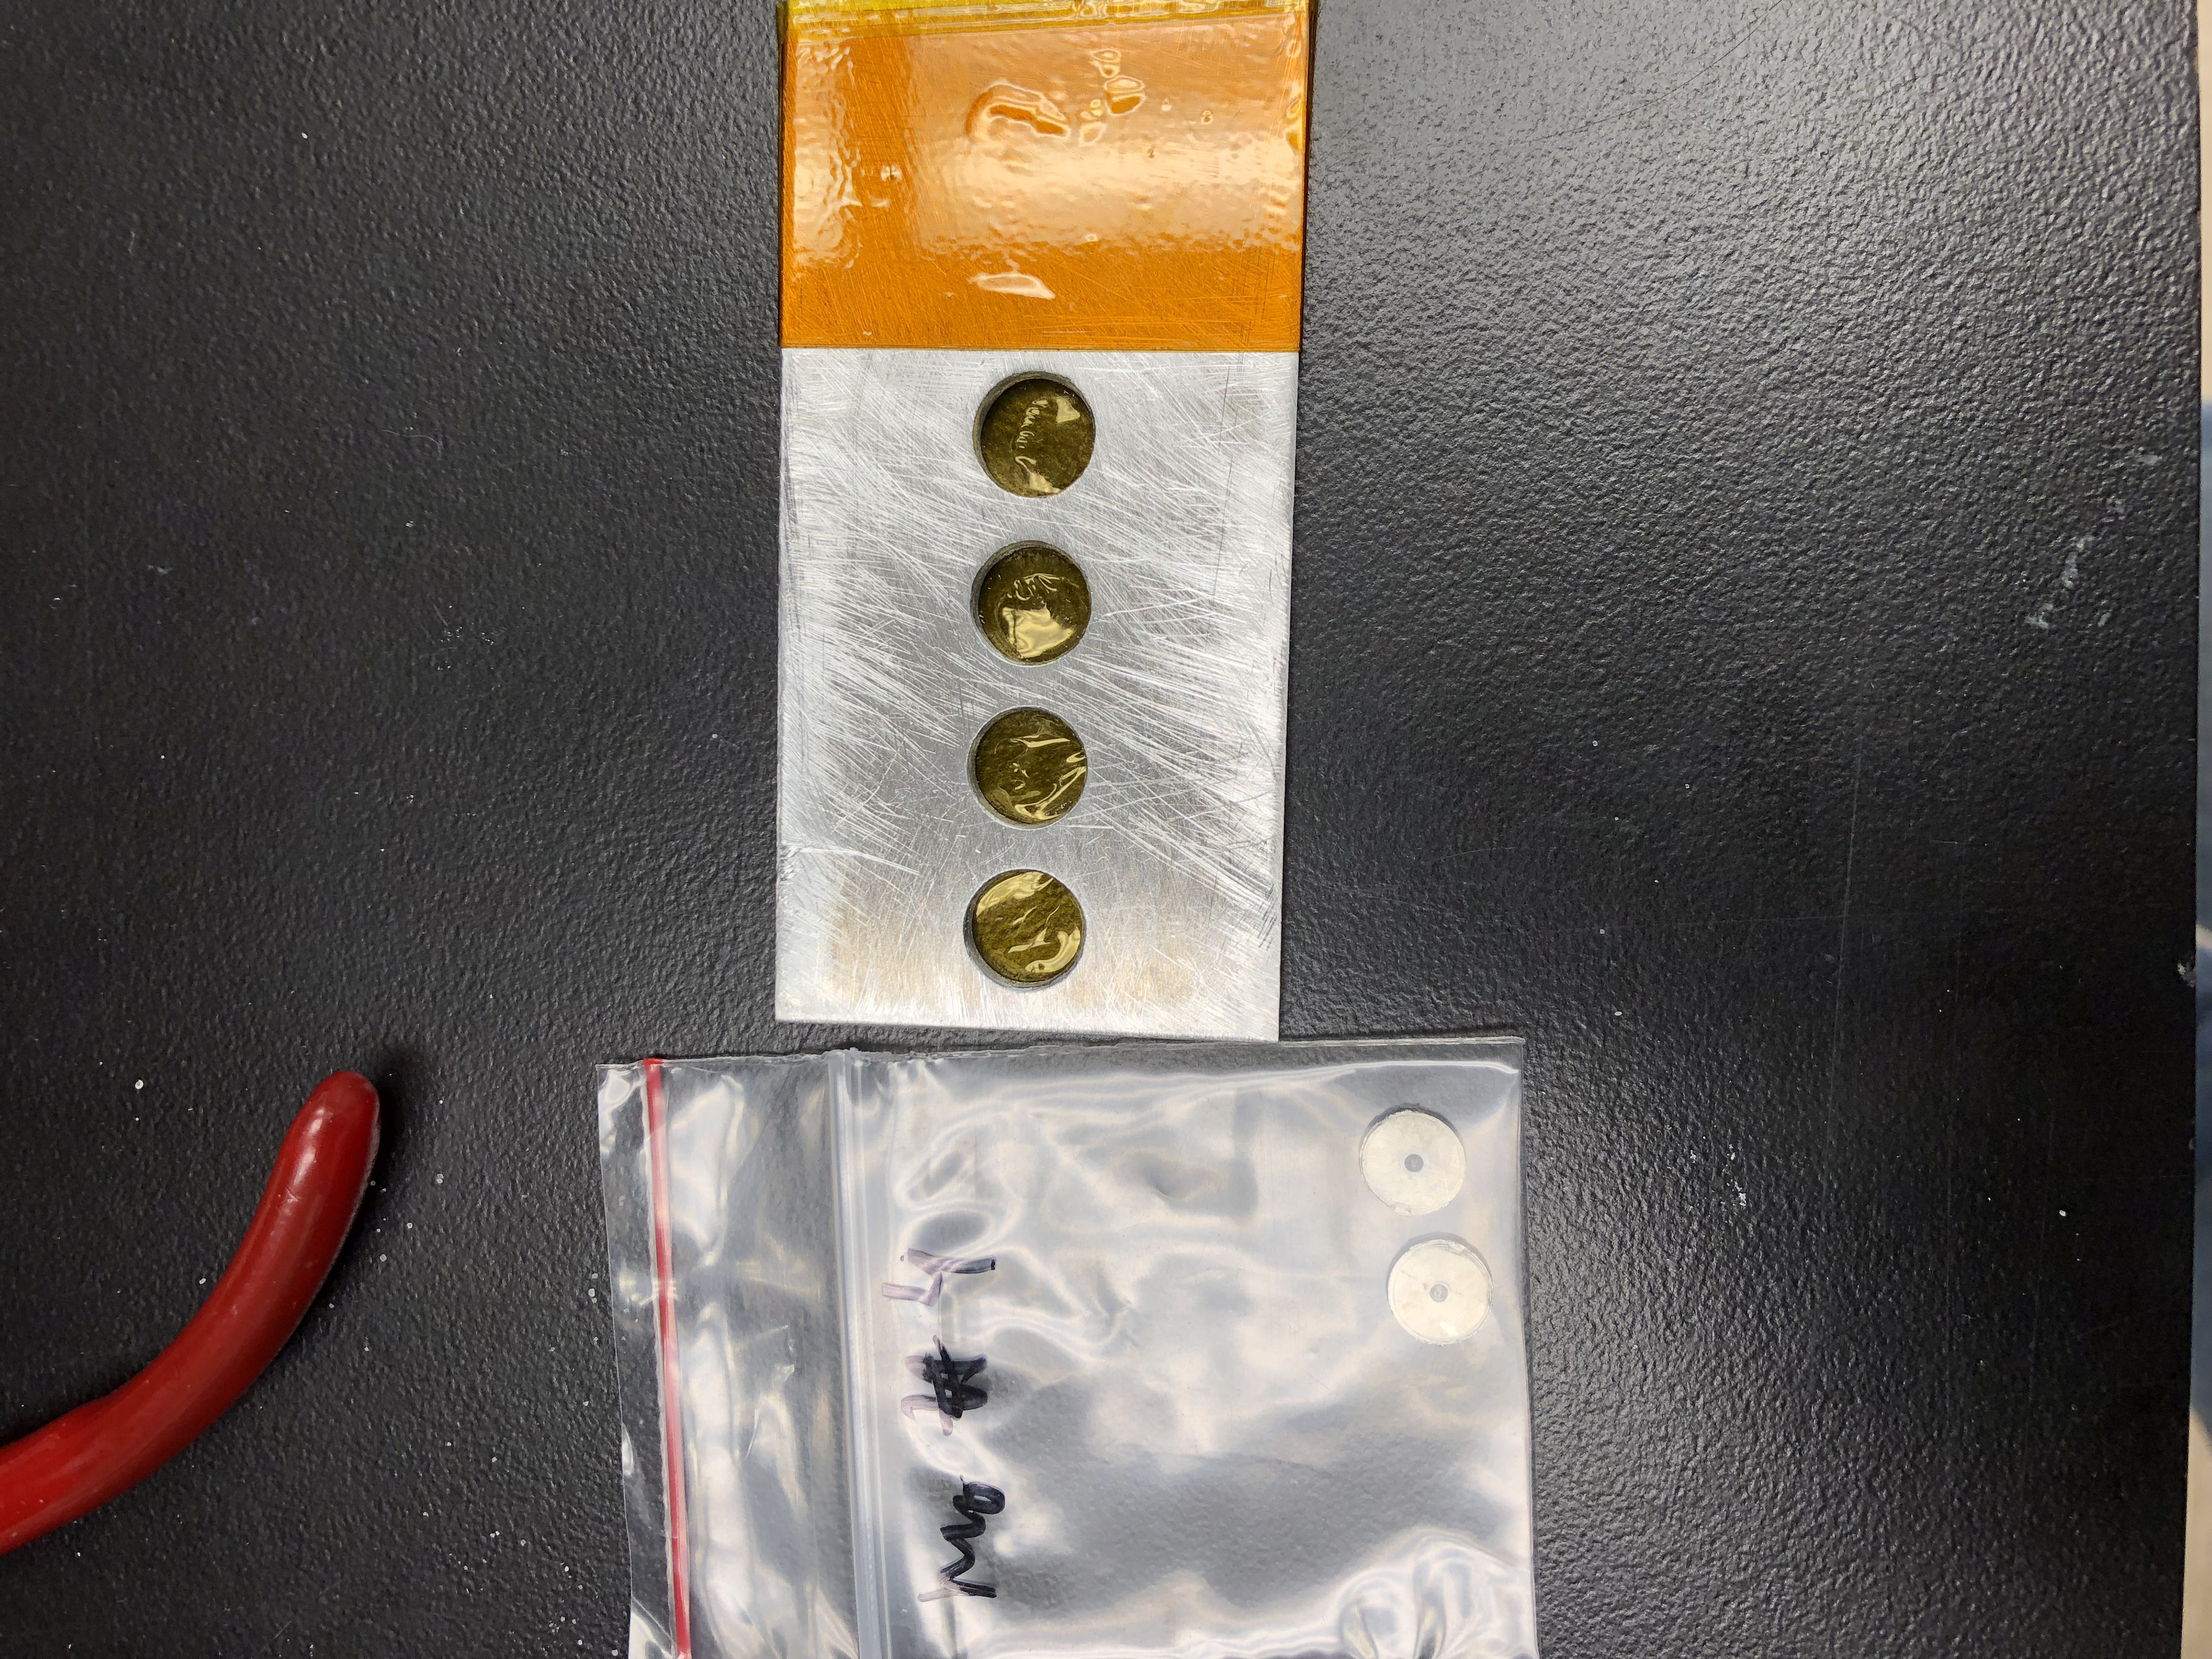
\includegraphics[clip=true,trim=5pt 1000pt 10pt 900pt,width=0.75\columnwidth,angle=90]{./figures/IMG_8840.JPG}
%  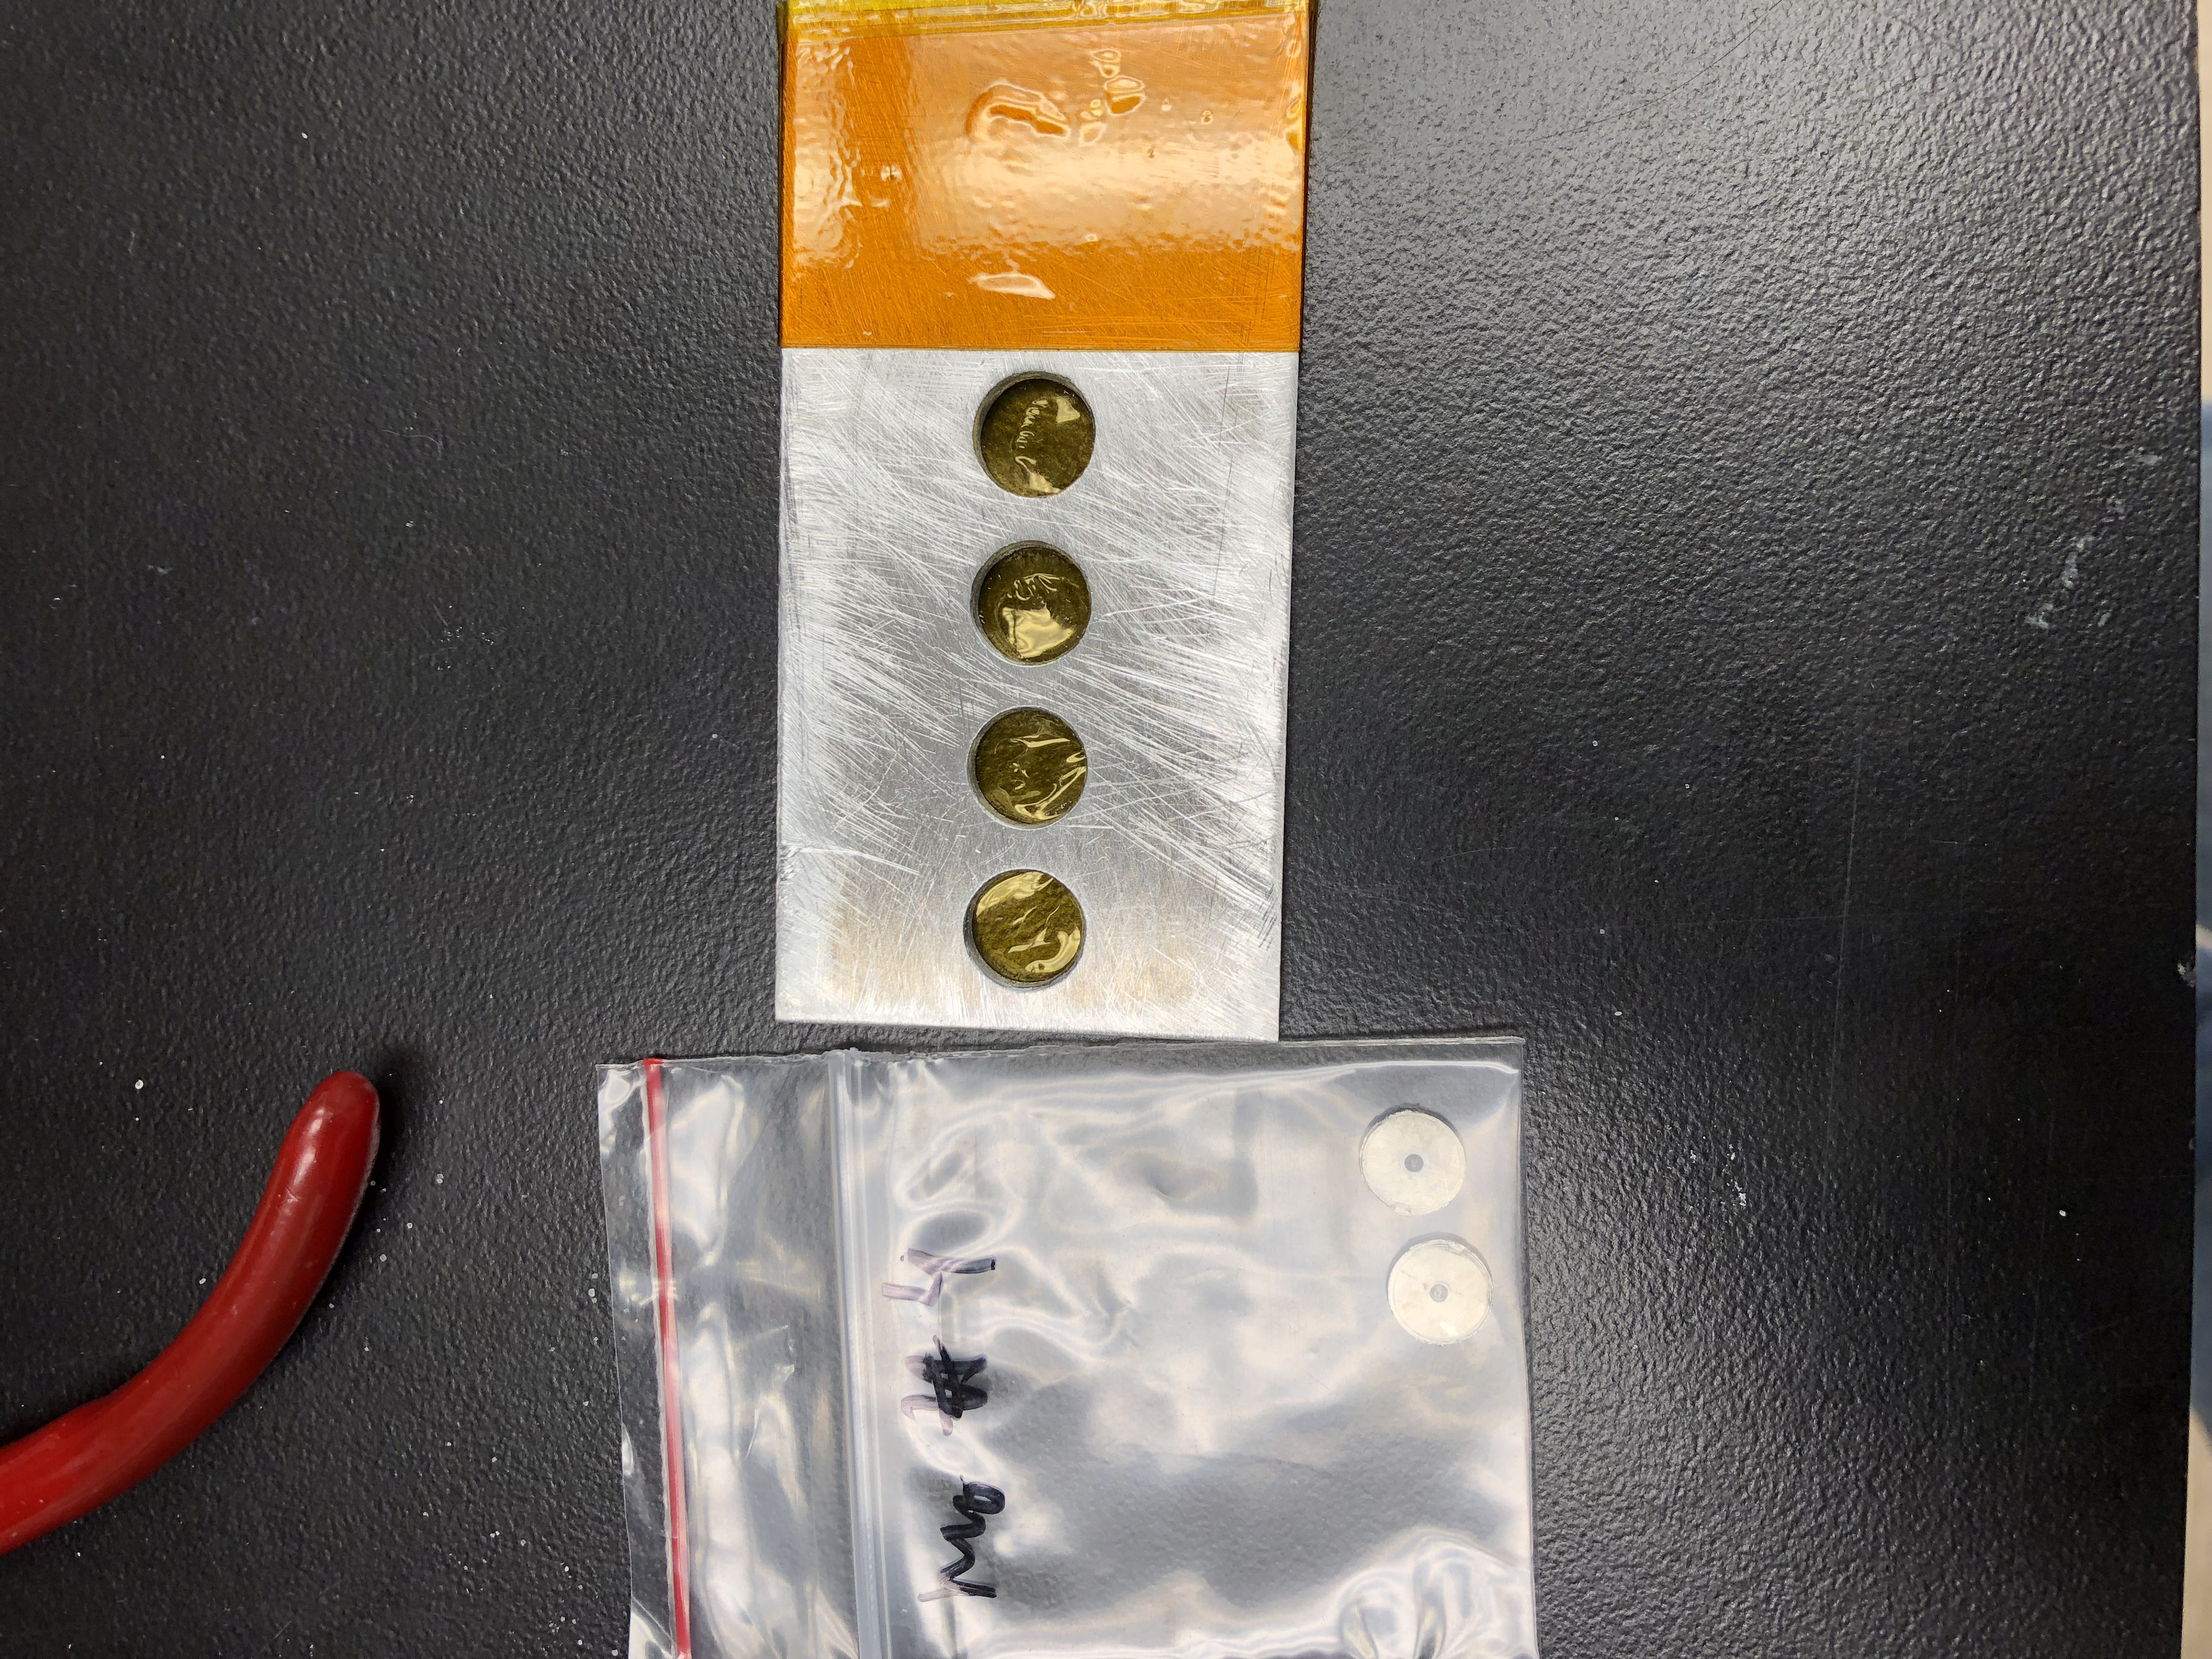
\includegraphics[width=0.75\columnwidth,angle=270]{./figures/IMG_8840.JPG}
%  \includegraphics[width=0.95\columnwidth]{./figures/Control Room Map.pdf}
 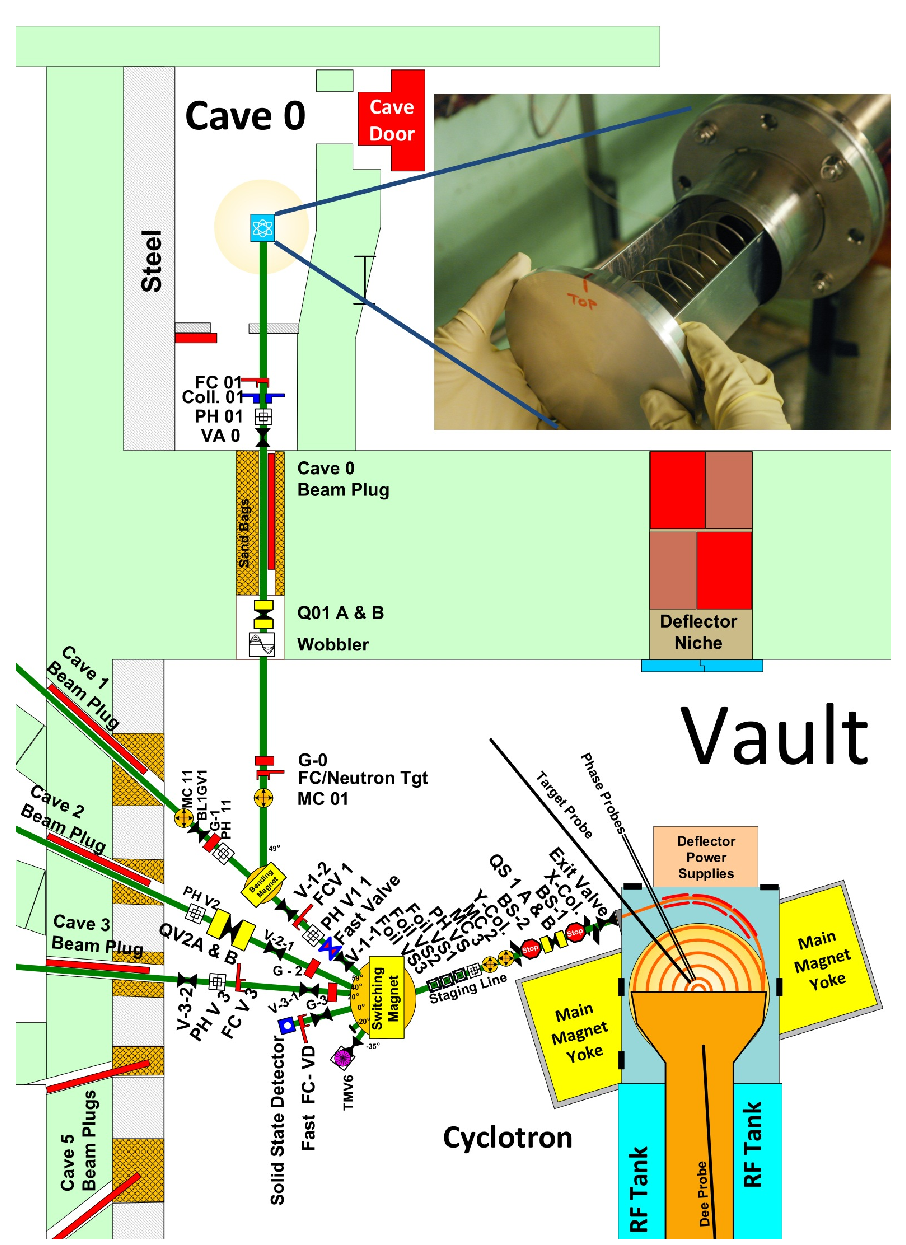
\includegraphics[height=0.90\textheight]{./figures/88beampath-cropped.pdf}
%  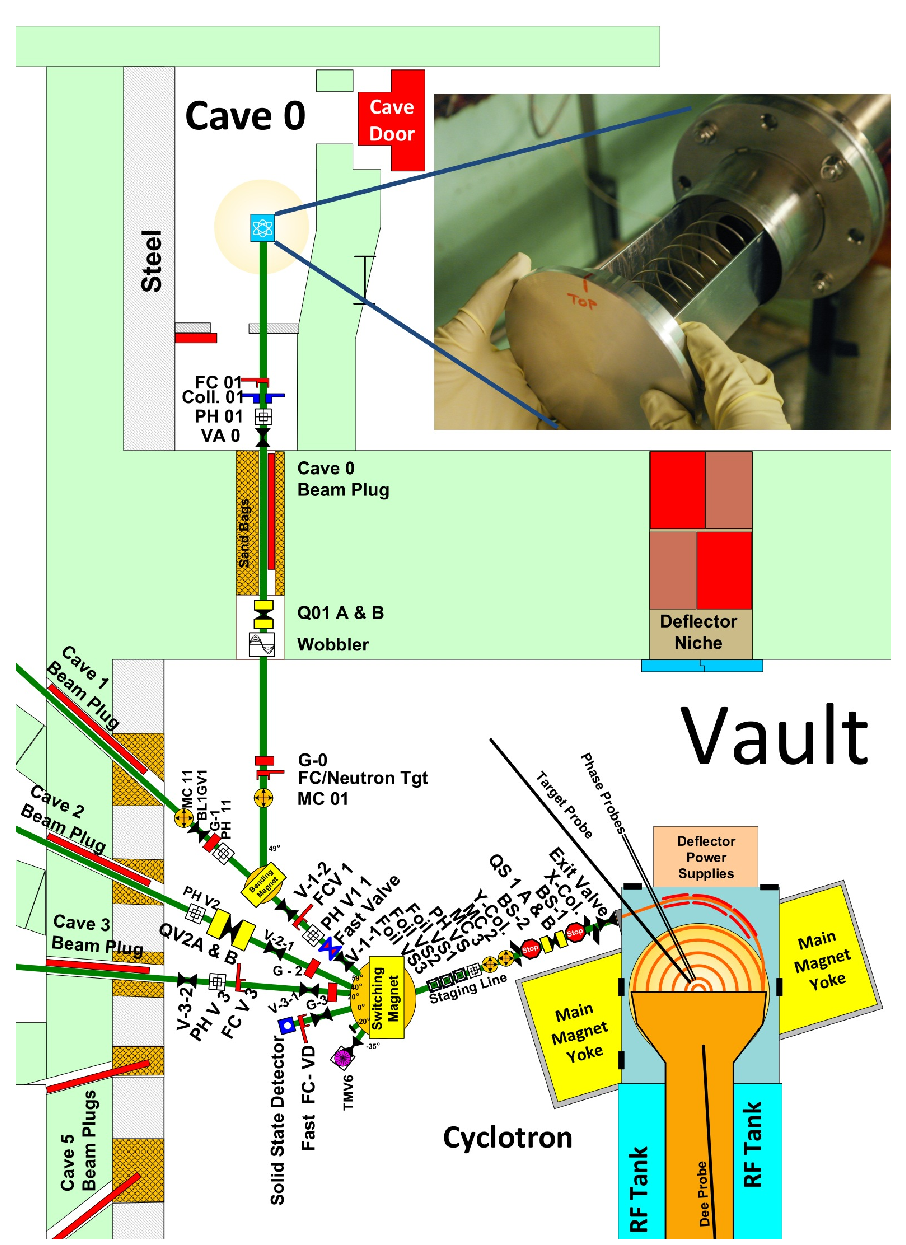
\includegraphics[width=0.95\columnwidth]{./figures/88beampath-cropped.pdf}
 % IMG_8840.JPG: 4032x3024 pixel, 72dpi, 142.24x106.68 cm, bb=0 0 4032 3024
 \caption{Schematic diagram of the 88-Inch Cyclotron facility and beamlines at LBNL, highlighting the beam path to Cave 0.  A rear view of the target stack holder used in this work is seen here, where it mounts onto the end of the Cave 0 beamline. }
 \label{fig:fe_beamline_schematic}
\end{figure}

% \begin{figure}
%  \centering
% %                                l   b      r    top
% %  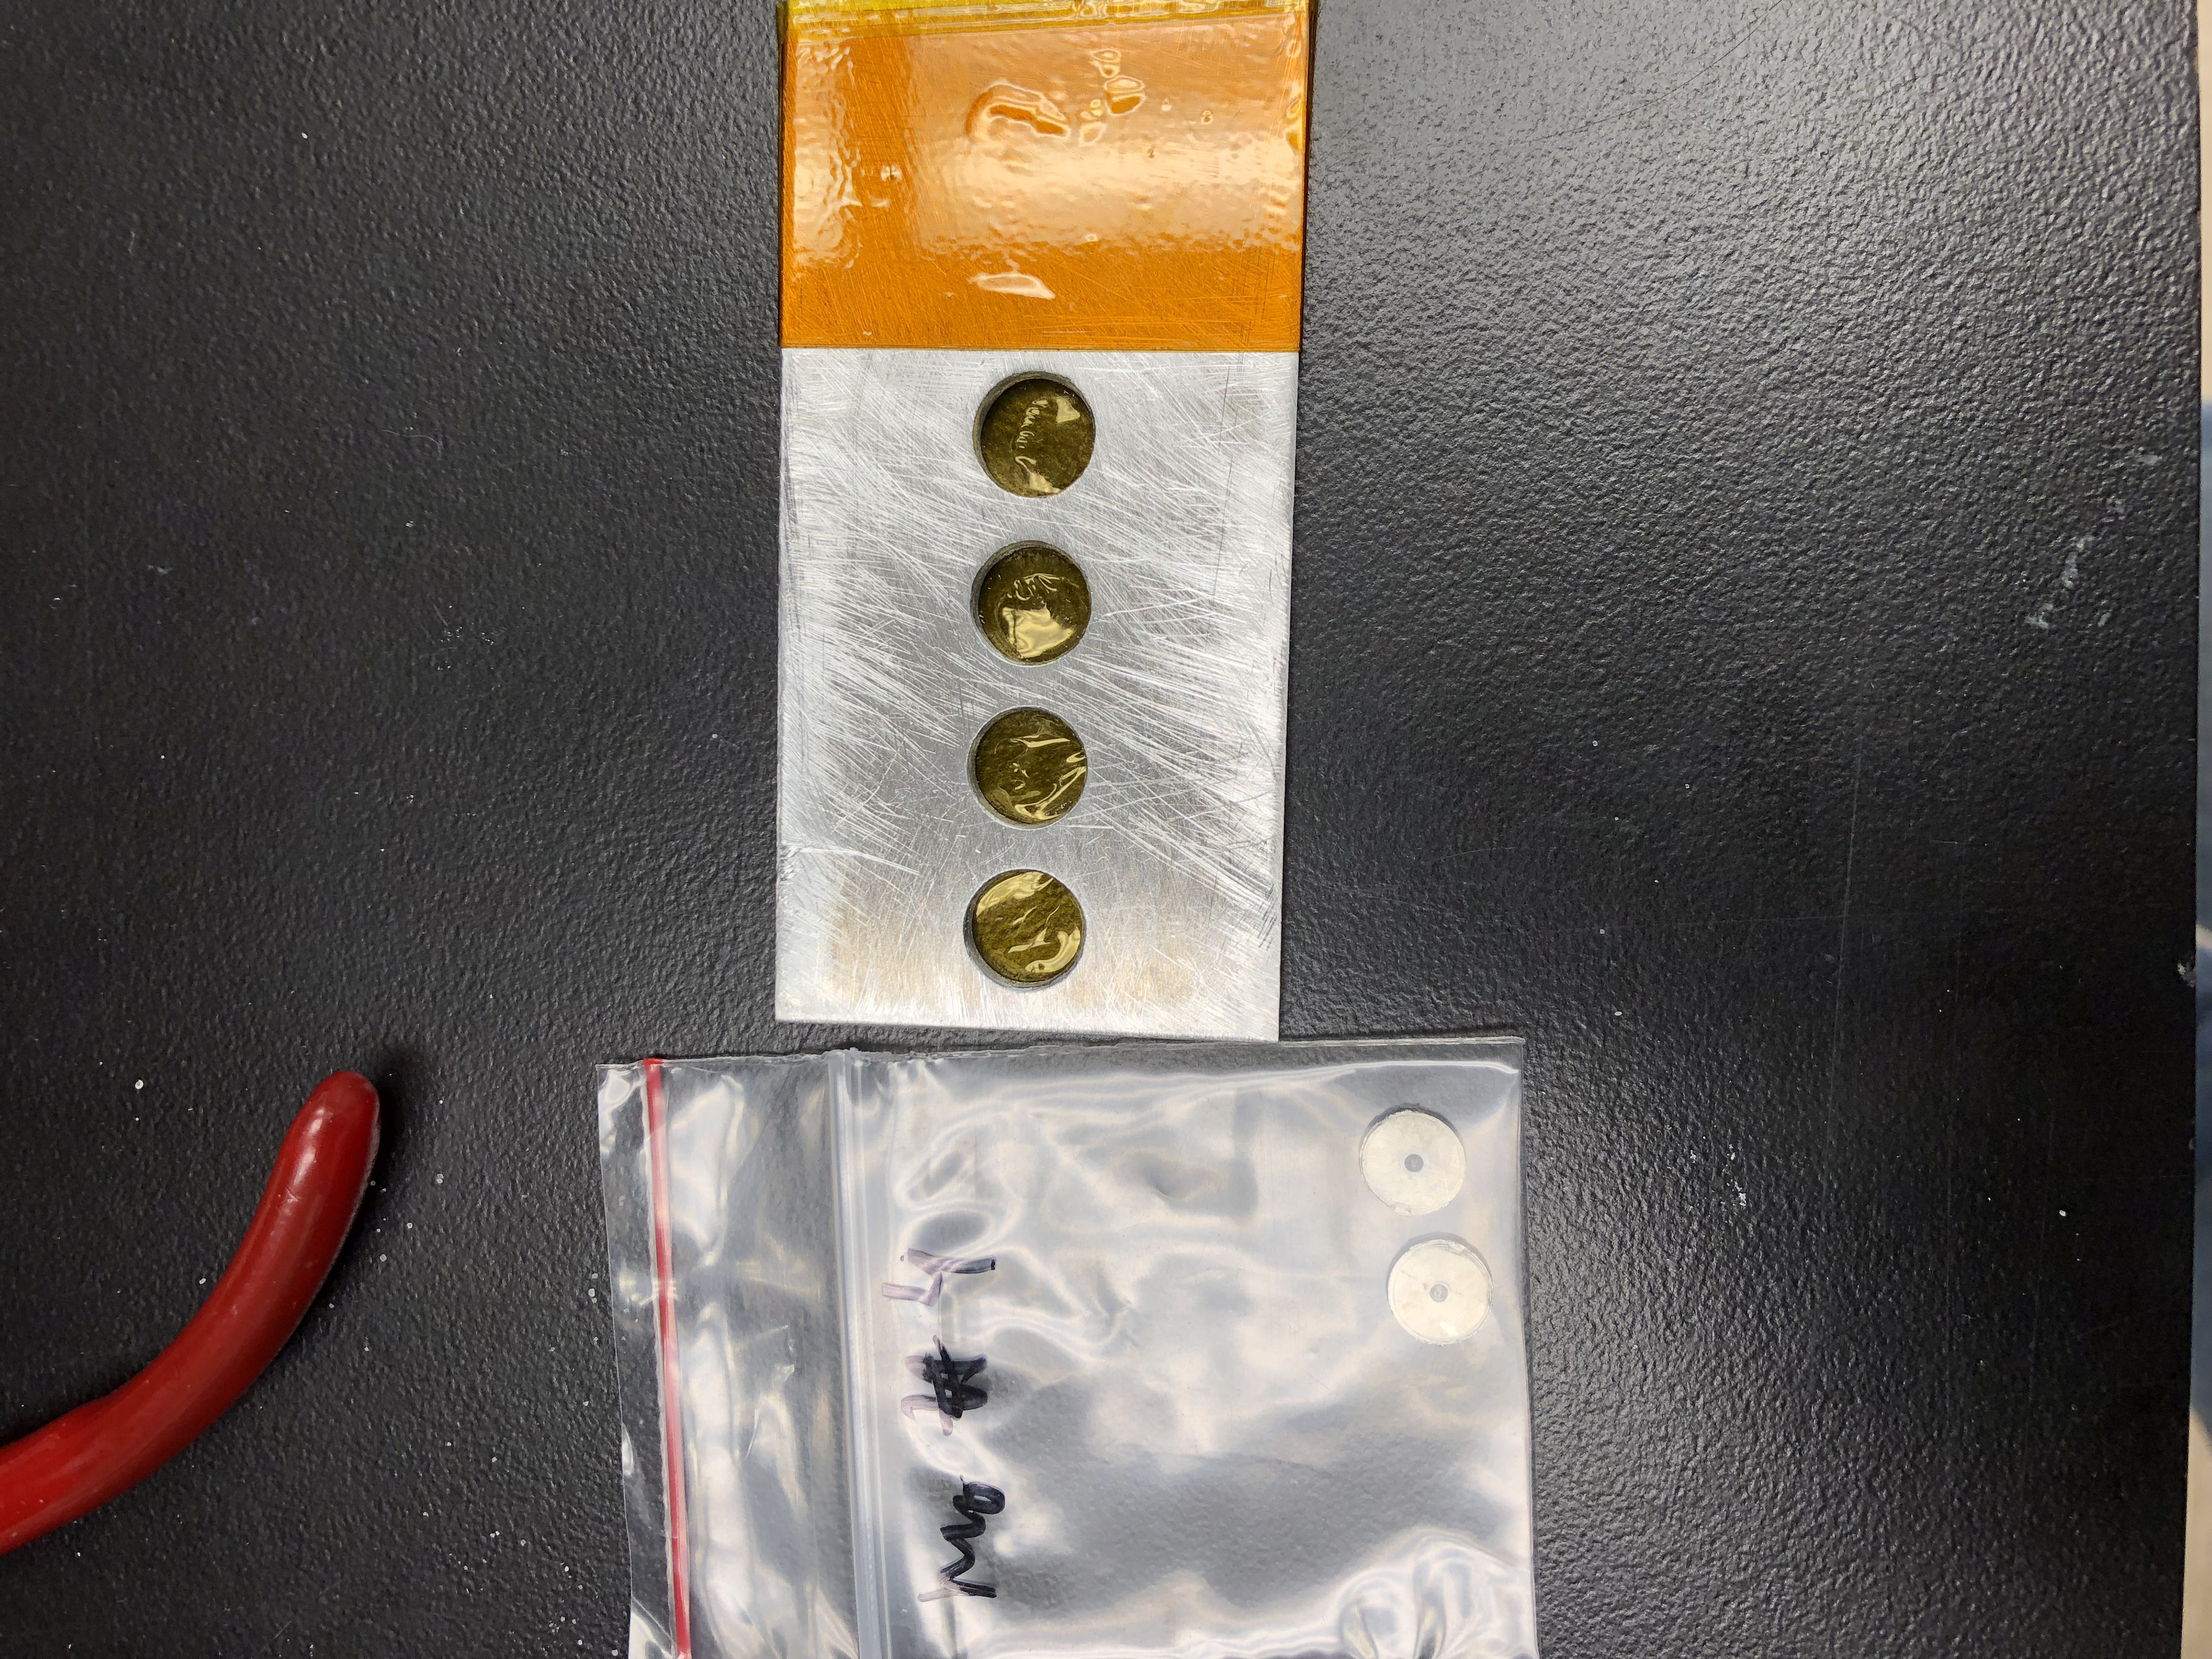
\includegraphics[clip=true,trim=5pt 1000pt 10pt 900pt,width=0.75\columnwidth,angle=90]{./figures/IMG_8840.JPG}
% %  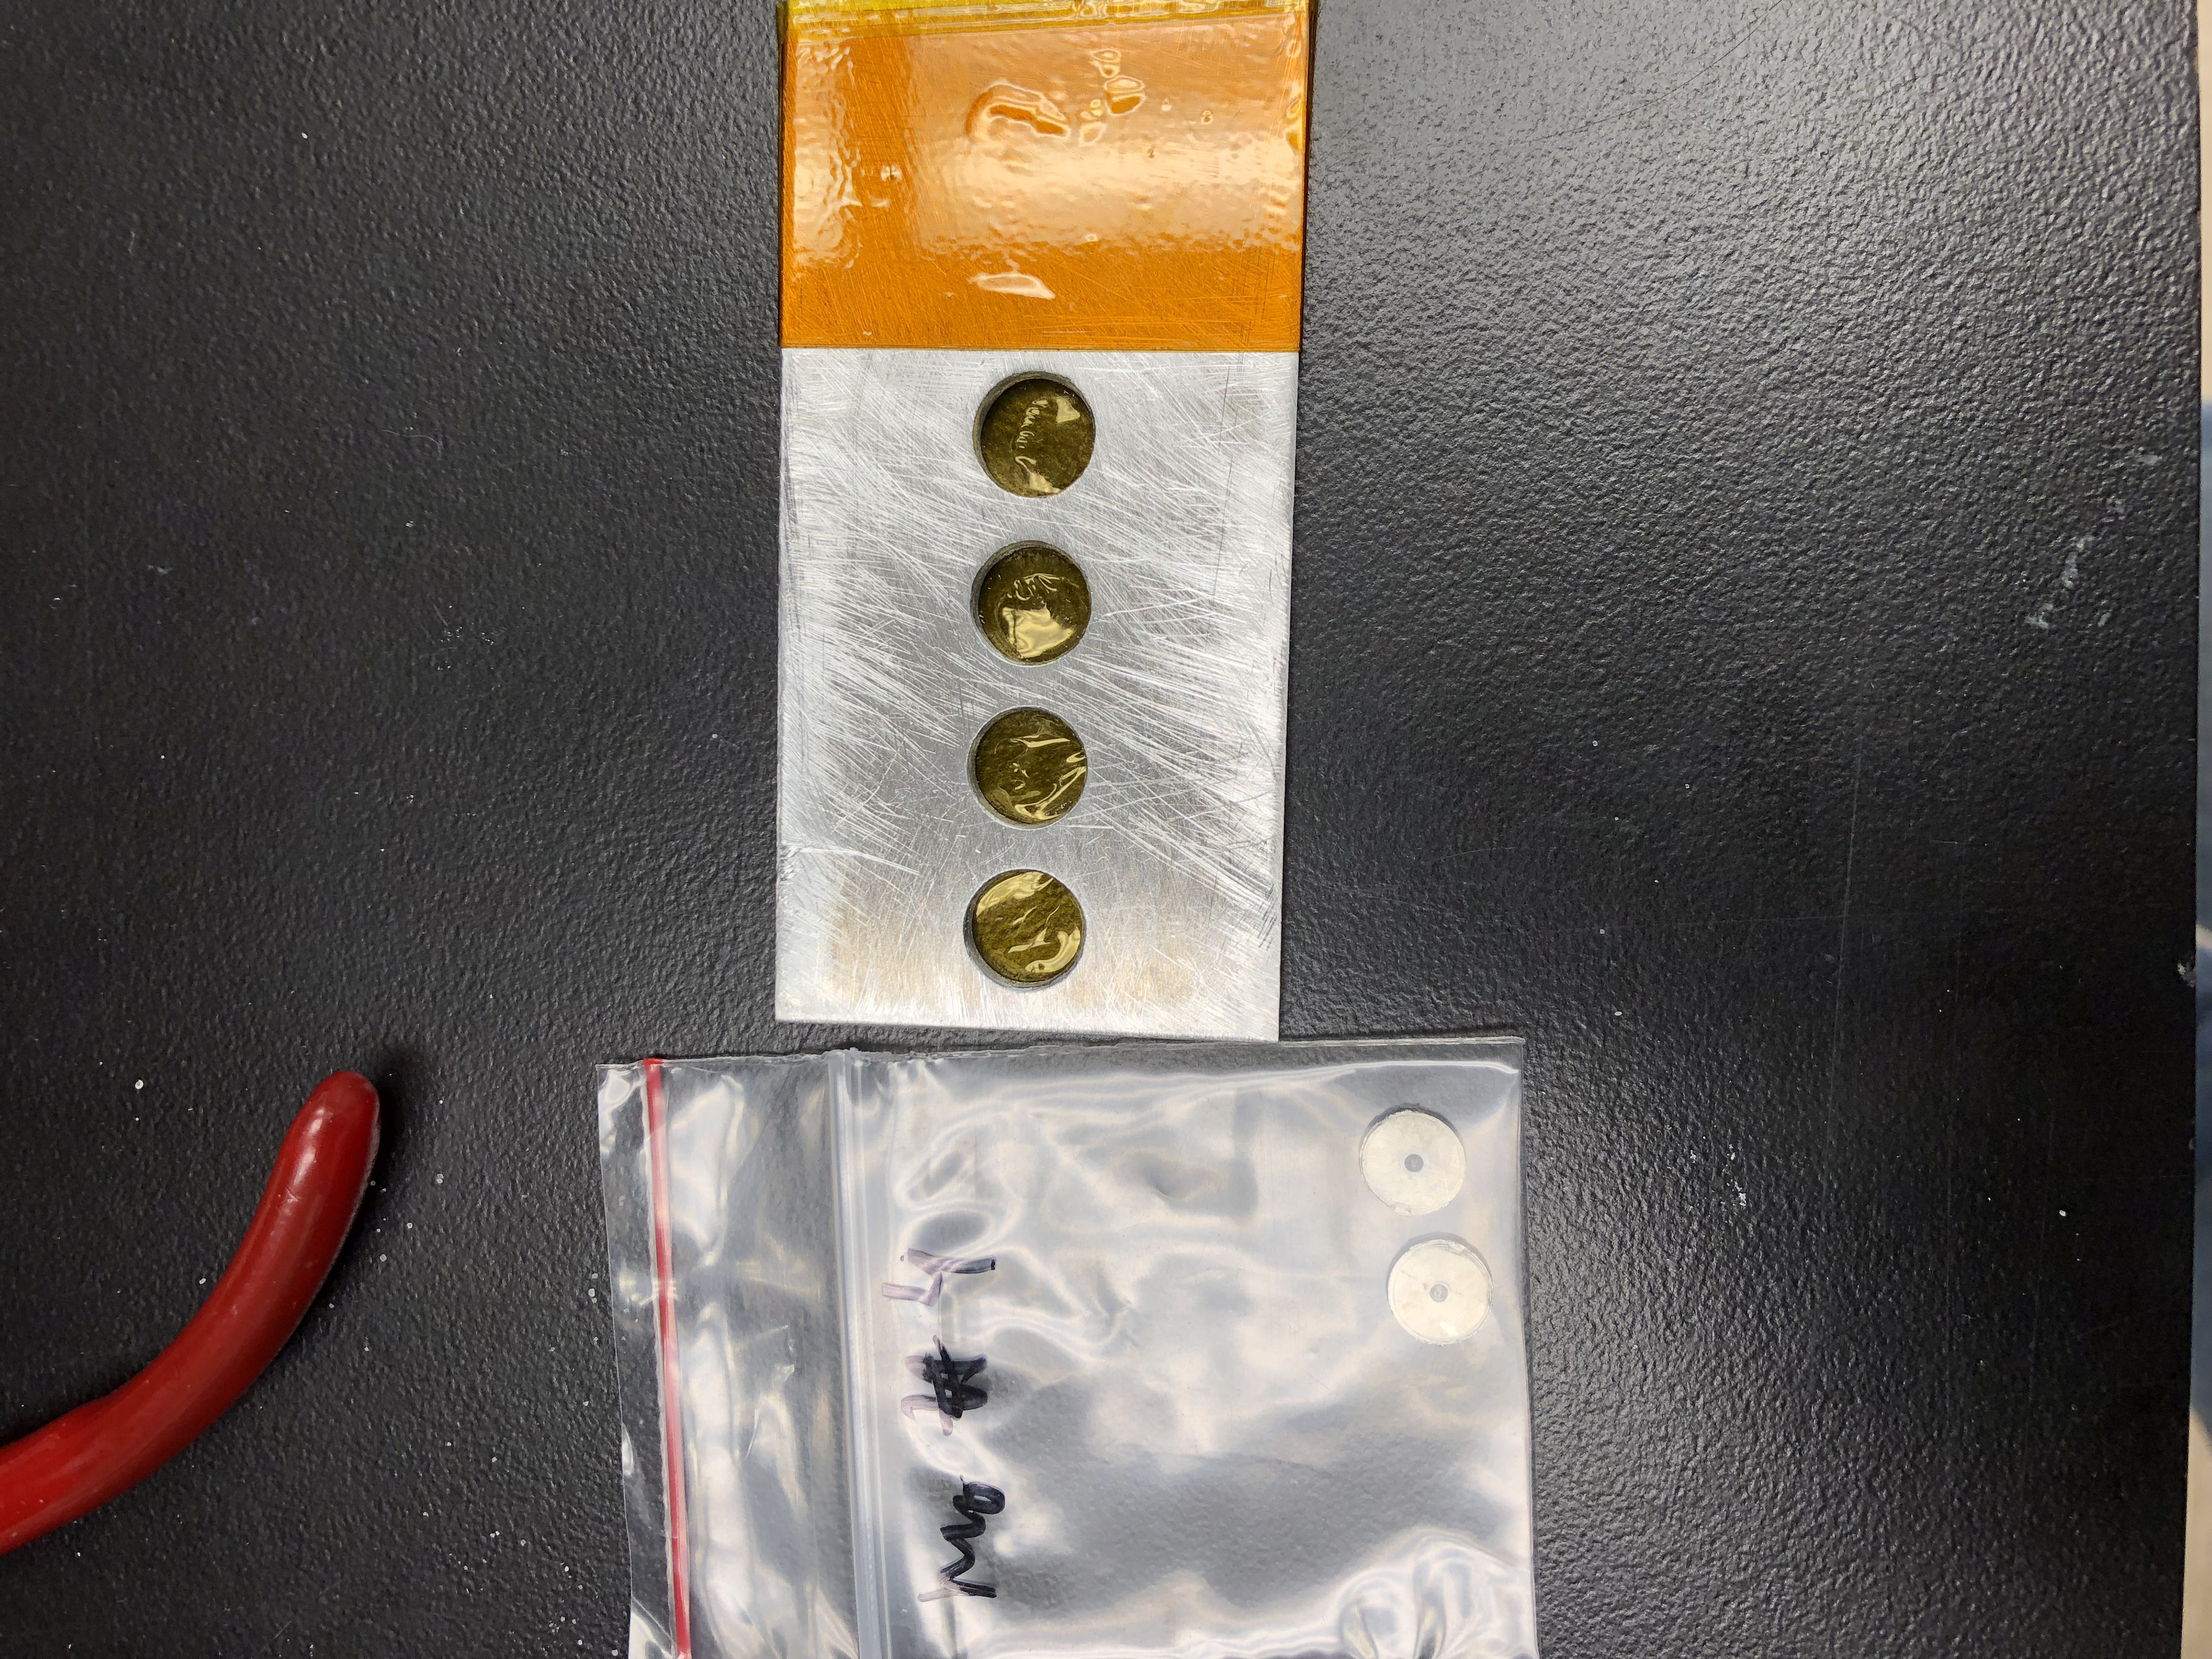
\includegraphics[width=0.75\columnwidth,angle=270]{./figures/IMG_8840.JPG}
%  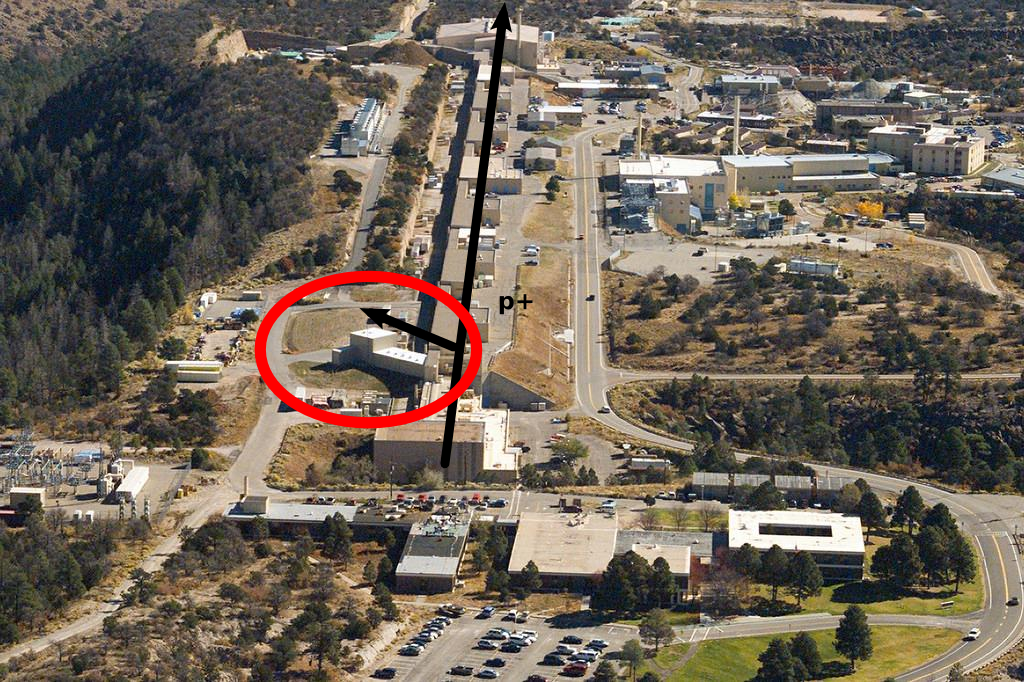
\includegraphics[width=0.75\columnwidth]{./figures/ipf_beamline_alternate.png}
%  % IMG_8840.JPG: 4032x3024 pixel, 72dpi, 142.24x106.68 cm, bb=0 0 4032 3024
%  \caption{Aerial photograph of the LANSCE beamline. Proton injectors are seen in the foreground building near the arrow's tail. The IPF beamline and operations facility is seen to the left of the main LANSCE beamline, circled in red.  The target box seen in \autoref{fig:target_stack} is lowered into the beamline here, via a hot cell.}
%  \label{fig:fe_beamline_alternate}
% \end{figure}





\subsubsection{Beam profile measurements}

% \textred{Verify that we used polyethylene!!!}



Following  tuning of the 25 and 55\,MeV proton beams into Cave 0, the  final remaining step prior to loading the  target box for irradiation is to tune the beam optics and spatial profile.
In the prior fielding run from April 2016, this was performed by loading 3 pieces of the EBT3 Gafchromic film (the same as used for imaging the beam  with stainless steel profile monitors) into the empty target stack holder, with one at the front end, one at the rear, and one in the middle.
At this point, the target stack would be mounted into the beamline, which would be pumped down to the \textred{200\,mtorr} beamline pressure for a run.
Following pumpdown, the \enquote{stack} of films would be exposed to an extremely short, low-current pulse of the tuned proton beam (approximately 0.1\,nAh for 1\,s), to directly expose the films and image the beam profile and optics.
Running any more beam fluence than this would cause the entire film to be massively overexposed, nullifying its usefulness.
At this point, the beamline would be brought up to atmosphere, and  the films removed for interpretation.
The cyclotron operator would then use the films to adjust the beam's horizontal and vertical position, and tune the beam optics to produce a \enquote{pencil-beam} spatial profile.
This is to ensure that the beam spot will be centered on the mounted target foils, and fully constrained within the foils, under-filling them.
After tuning the beam's optics, more films would be loaded, and this process would be repeated multiple times, confirming any adjustments made to improve the optics, until an acceptable beam spot was achieved. 
Each cycle of loading and unloading a set of films would take approximately 45\,min, followed by approximately another 30\,min to make any beam adjustments, followed by the 1\,s film exposure.
As a result, during this fielding run, optical tuning took nearly an entire day of beam time, which would be infeasible for future experiments.


To improve this process, I designed a phosphor target to mount into the end of the beamline during optics tuning, sealing onto the beamline during pumpdown via an inset o-ring.
This design was based off of designs for the beam stop component of the target stack holder, but instead of featuring a solid aluminum end cap, it has a circular opening, designed to hold a glass puck.
This puck forms a vacuum seal through an inset o-ring, and is held against the rear of the target by an aluminum frame.
The blueprints for this phosphor are seen in \autoref{fig:fe_phosphor}.
On the inside (beamline-facing) side of the glass puck, a thin layer of vacuum greased was painted on, and mixed with a powdered phosphorescent paint, to create a thin phosphorescent layer.
This target is mounted onto the end of the beamline during optics tuning, and has been used in all experiments since.
When exposed to a low-current (approximately 0.1\,nAh) beam, the phosphor glows brightly, outlining the beam profile.
A low current is used, to ensure that the phosphor layer does not get overly heated and burn or flake off during tuning.
By patching in a camera to the cave, the operators may tune the beam optics in real time, moving the beam spot and improving its spatial profile, while watching on a video feed from the remote camera.
This has drastically shorted the optics tuning process down to less than a single hour, and has made all subsequent experiments far easier in the process.
A remote view of this phosphor target during tuning is seen in \autoref{fig:fe_preexp_beam_spot}.



\begin{figure}
    \centering
    \subfloat{
        \centering
%         \includegraphics[width=\columnwidth]{./figures/Capture.PNG}
        \hspace{-1pt}\subfigimg[width=0.925\textwidth]{a)}{./figures/Phosphor_Cap_Blueprints.pdf}{50}
%         \caption{ Decay curve for the isomeric transition of \ce{^{115m}In}.}
         %         \refstepcounter{subfigure}
%          \label{fig:fe_before_minimization}
   \hspace{-5pt}}%
     \subfloat{
        \centering
\\
%         \subfigimg[width=0.5\textwidth]{b)}{./figures/after_minimization_plot.pdf}{50}
        \subfigimg[width=0.4\textwidth]{\textcolor{white}{b)}}{./figures/perspective.png}{50}
         %         \refstepcounter{subfigure}
%          \label{fig:fe_after_minimization}
   \hspace{-5pt}}%
    \caption{Blueprints (a) and 3D cutaway rendering (b) of the phosphor target used for real-time beam optics tuning at the 88-Inch Cyclotron.} 
%     Following minimization, additional apparent fluence is observed in the  \ce{^{nat}Al}(p,x)\ce{^{22}Na} and \ce{^{nat}Al}(p,x)\ce{^{24}Na} monitor channels, due to contamination from \ce{^{nat}Si}(p,x)\ce{^{22,24}Na} on the silicone adhesive used for sealing foil packets.}
     \label{fig:fe_phosphor}
\end{figure}


However, this phosphor target offers a fairly low-resolution image of the beam profile, mostly useful as a qualitative guide for tuning.
As a result, a final film exposure is done after beam, optics appear satisfactory on the phosphor, to confirm the optics tune.
After verifying that 
% loading a sheet of polyethylene (approximately 3\,mm thick) into the the IPF beamline, at the same location of the target box's beam entrance window. 
% This sheet acts as a beam profile monitor, and is irradiated with 5 \mmicro A-min of the proton beam.
% Following exposure, the polyethylene monitor is withdrawn back into the IPF hot cell, where it is inspected to verify the shape and location of the beam profile.
% These beam profile irradiations leave an annealable discoloration of the beam profile, which resembles a \enquote{burn mark}, and are observed to passively revert within 1--2 weeks.
% The final pre-irradiation beam spot from the Nb(p.x) measurement is seen in  \autoref{fig:ipf_preexp_beam_spot}.
% LANSCE accelerator operations staff use this feedback to fine-tune the beam, 
the beam spot is centered upon the target stack and focusing it to ensure that it underfills the target foils, the foils are loaded into the stack target holder, mounted in the beamline, and the irradiation commences.
 








\begin{figure}
 \centering
%                                l   b      r    top
%  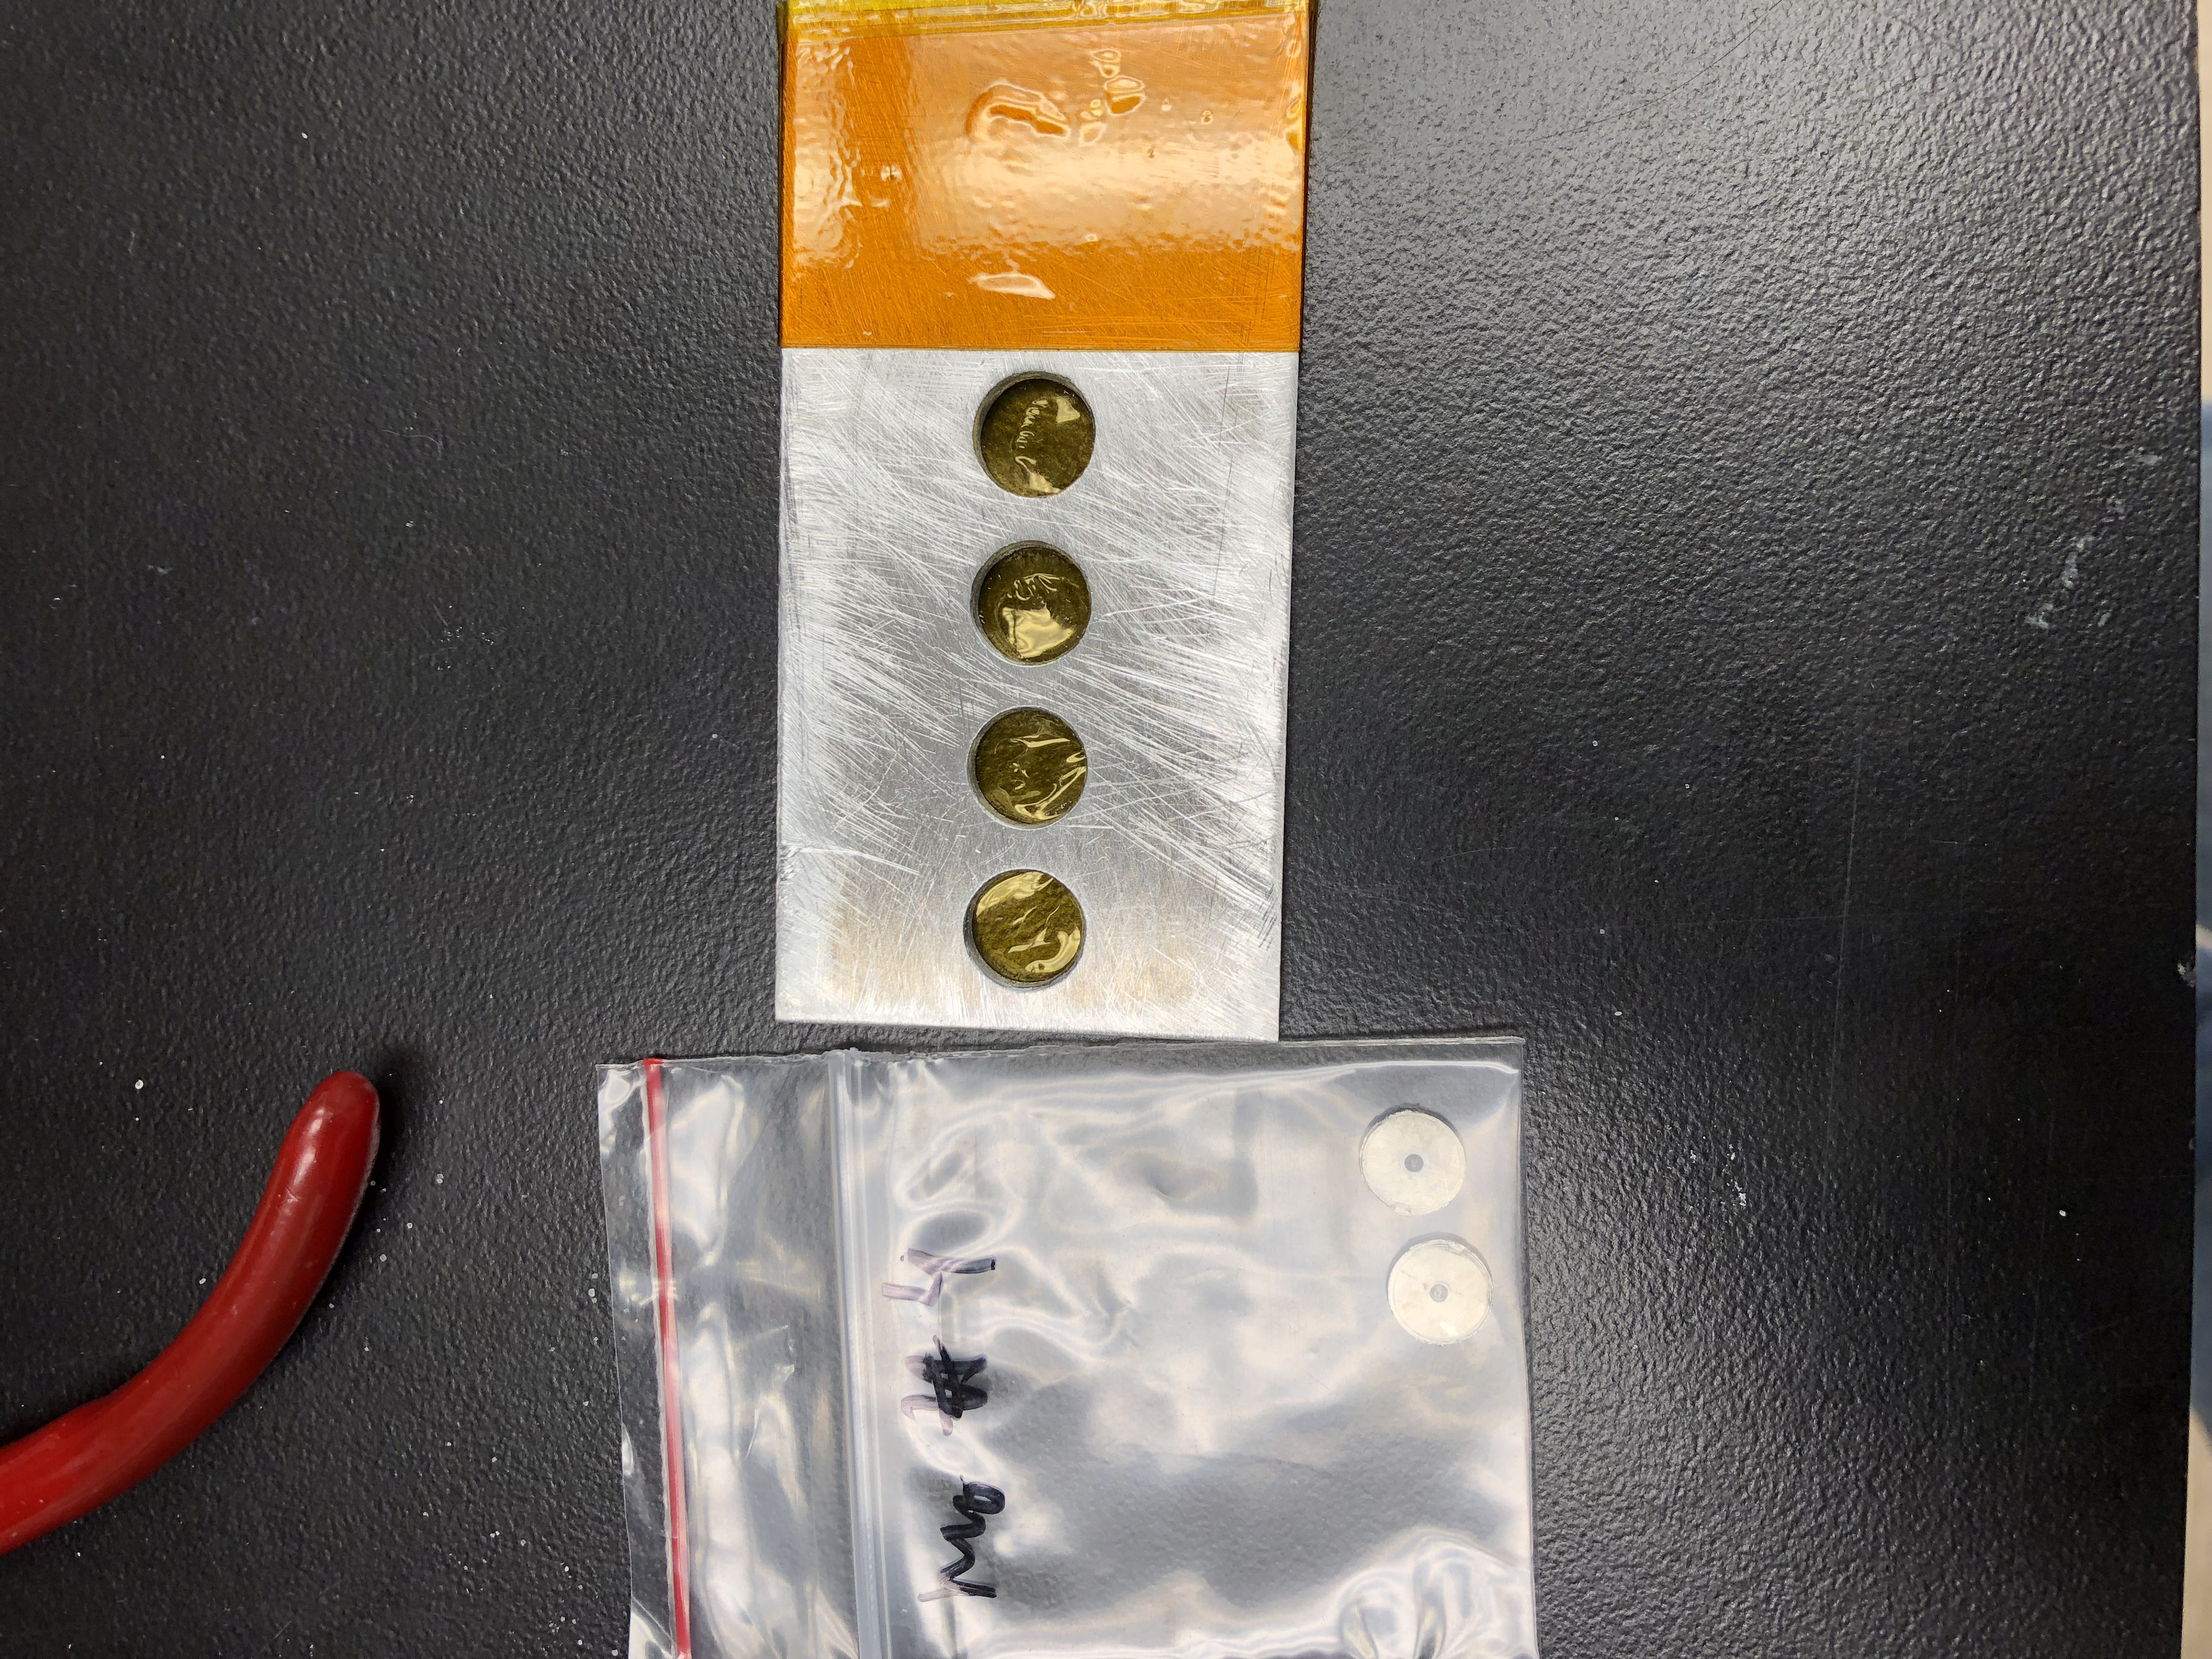
\includegraphics[clip=true,trim=5pt 1000pt 10pt 900pt,width=0.75\columnwidth,angle=90]{./figures/IMG_8840.JPG}
%  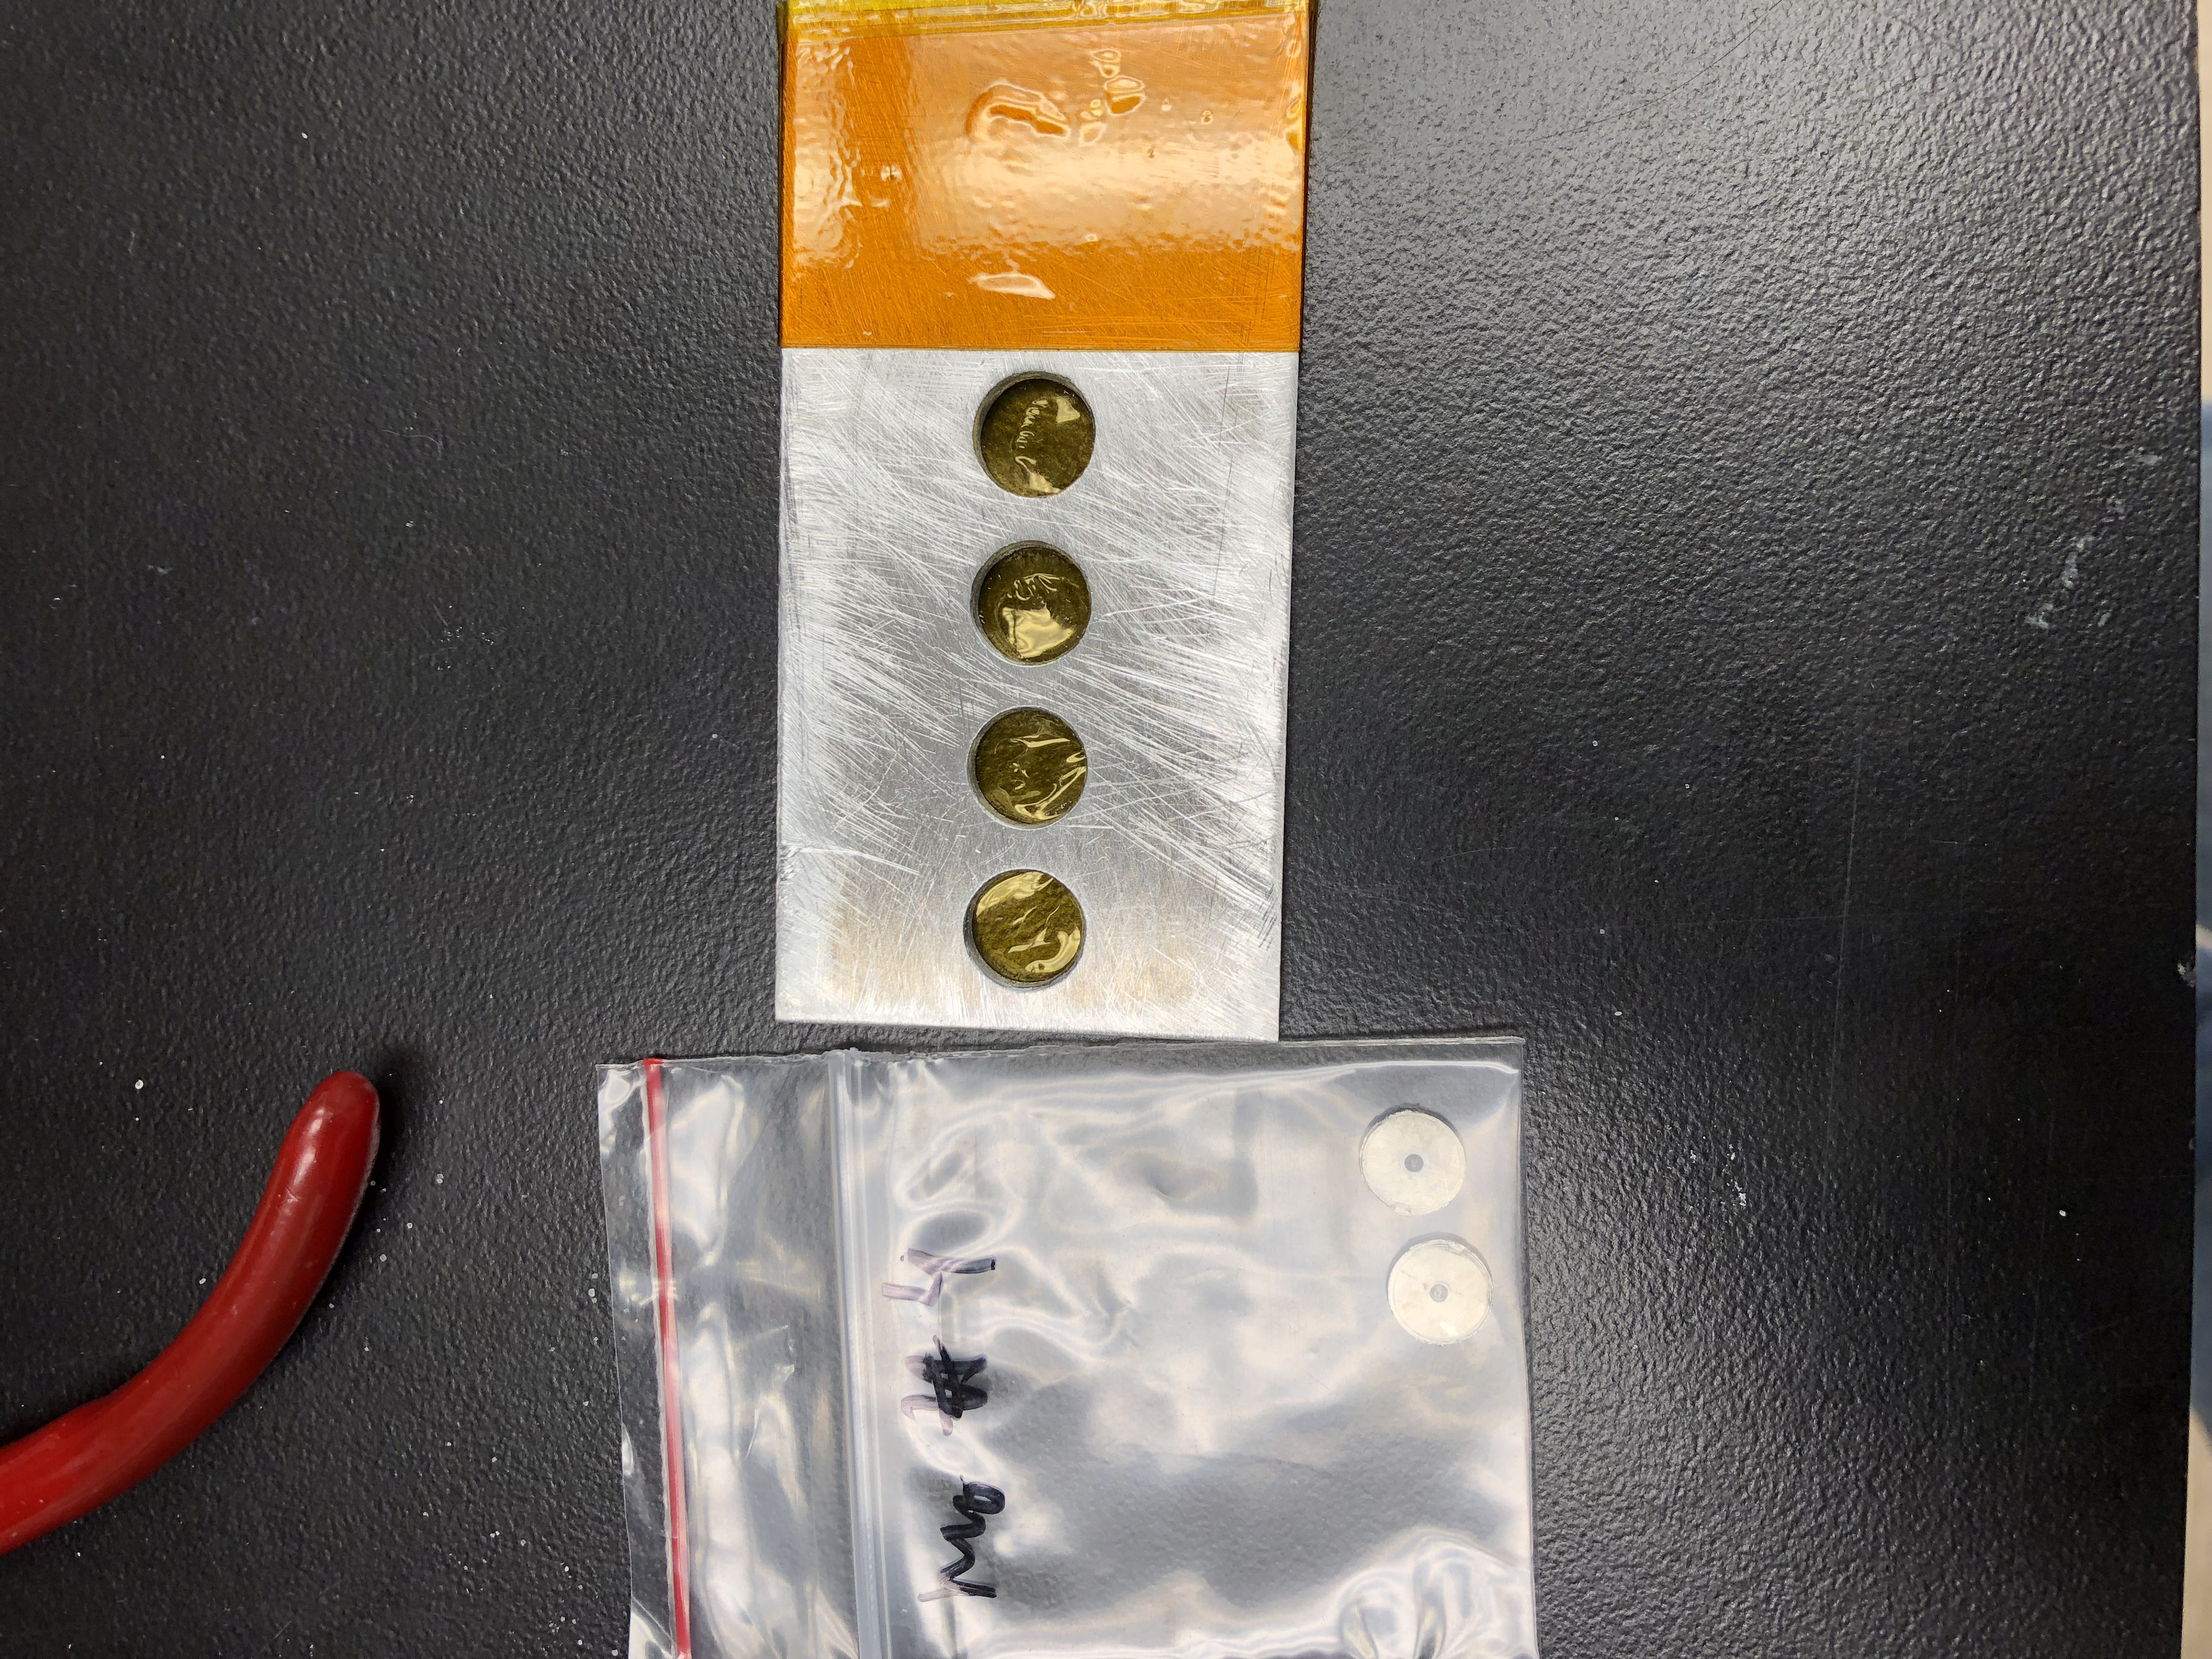
\includegraphics[width=0.75\columnwidth,angle=270]{./figures/IMG_8840.JPG}
 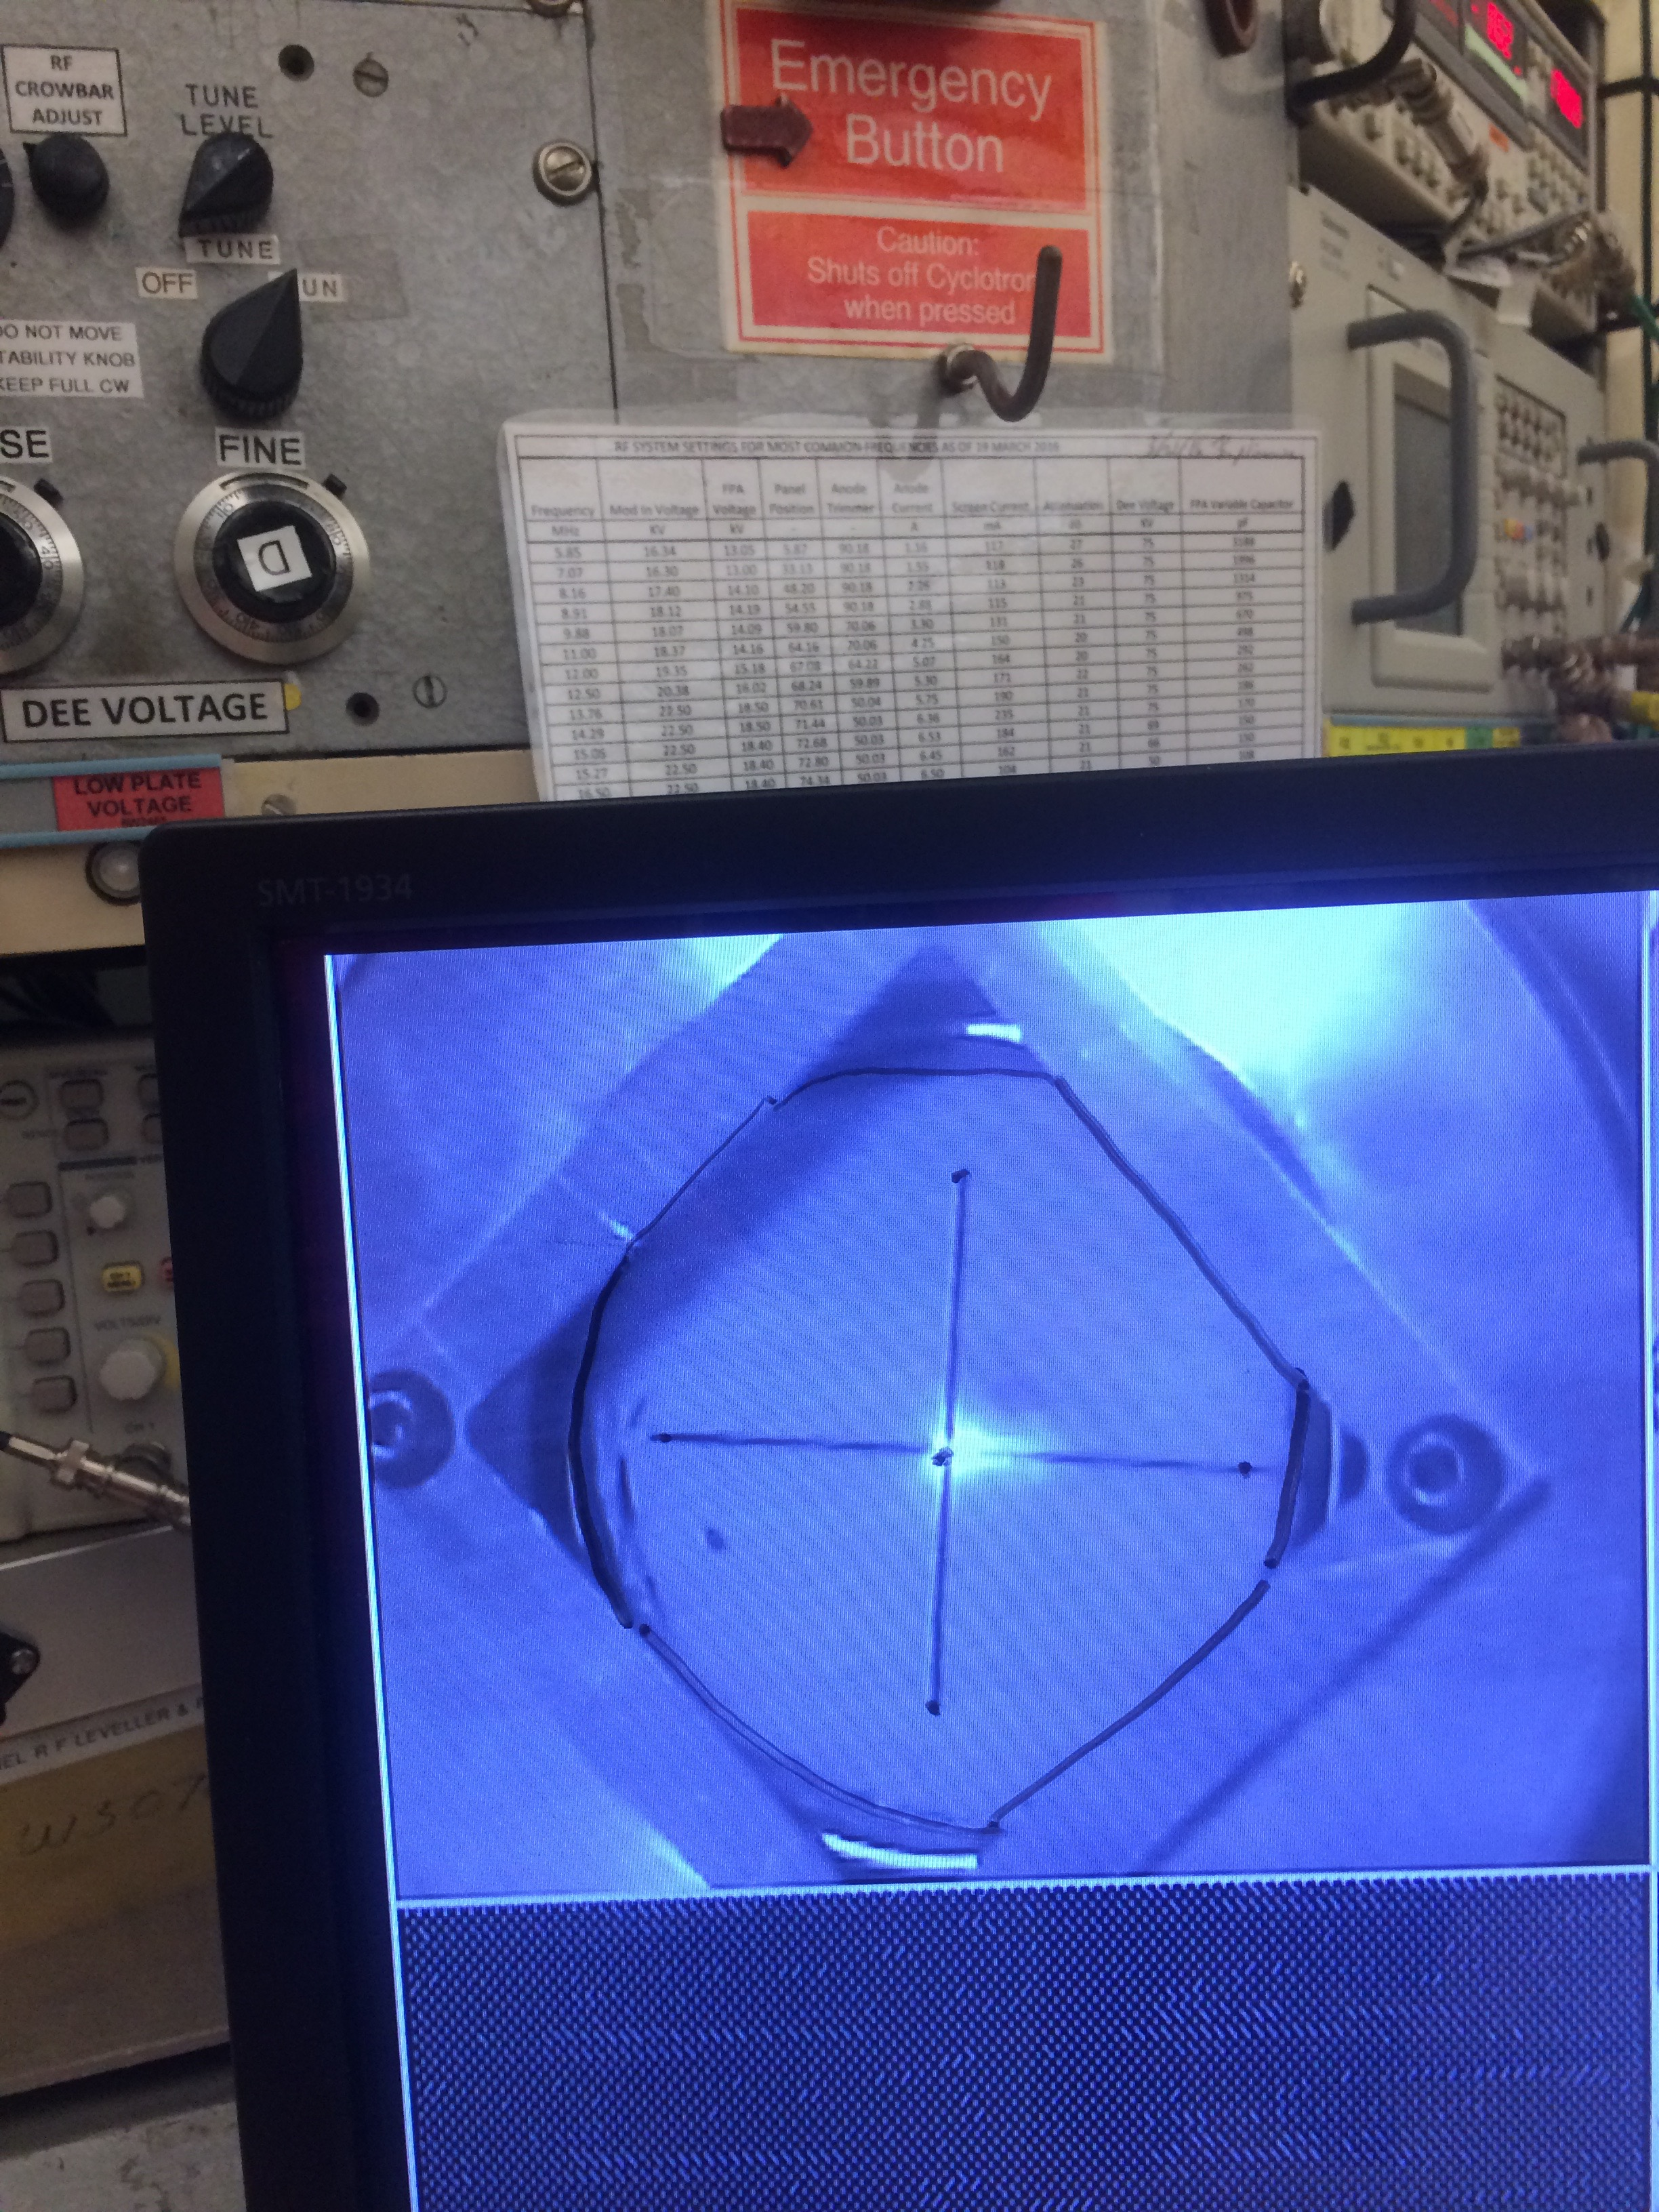
\includegraphics[width=0.75\columnwidth]{./figures/IMG_0337.jpg}
 % IMG_8840.JPG: 4032x3024 pixel, 72dpi, 142.24x106.68 cm, bb=0 0 4032 3024
 \caption{View of the remote feed of the phosphor target during beam optics tuning. The low-current proton beam used for tuning is visible as the bright glow around the reference crosshairs.}
 \label{fig:fe_preexp_beam_spot}
\end{figure}



\begin{figure}
 \centering
%                                l   b      r    top
%  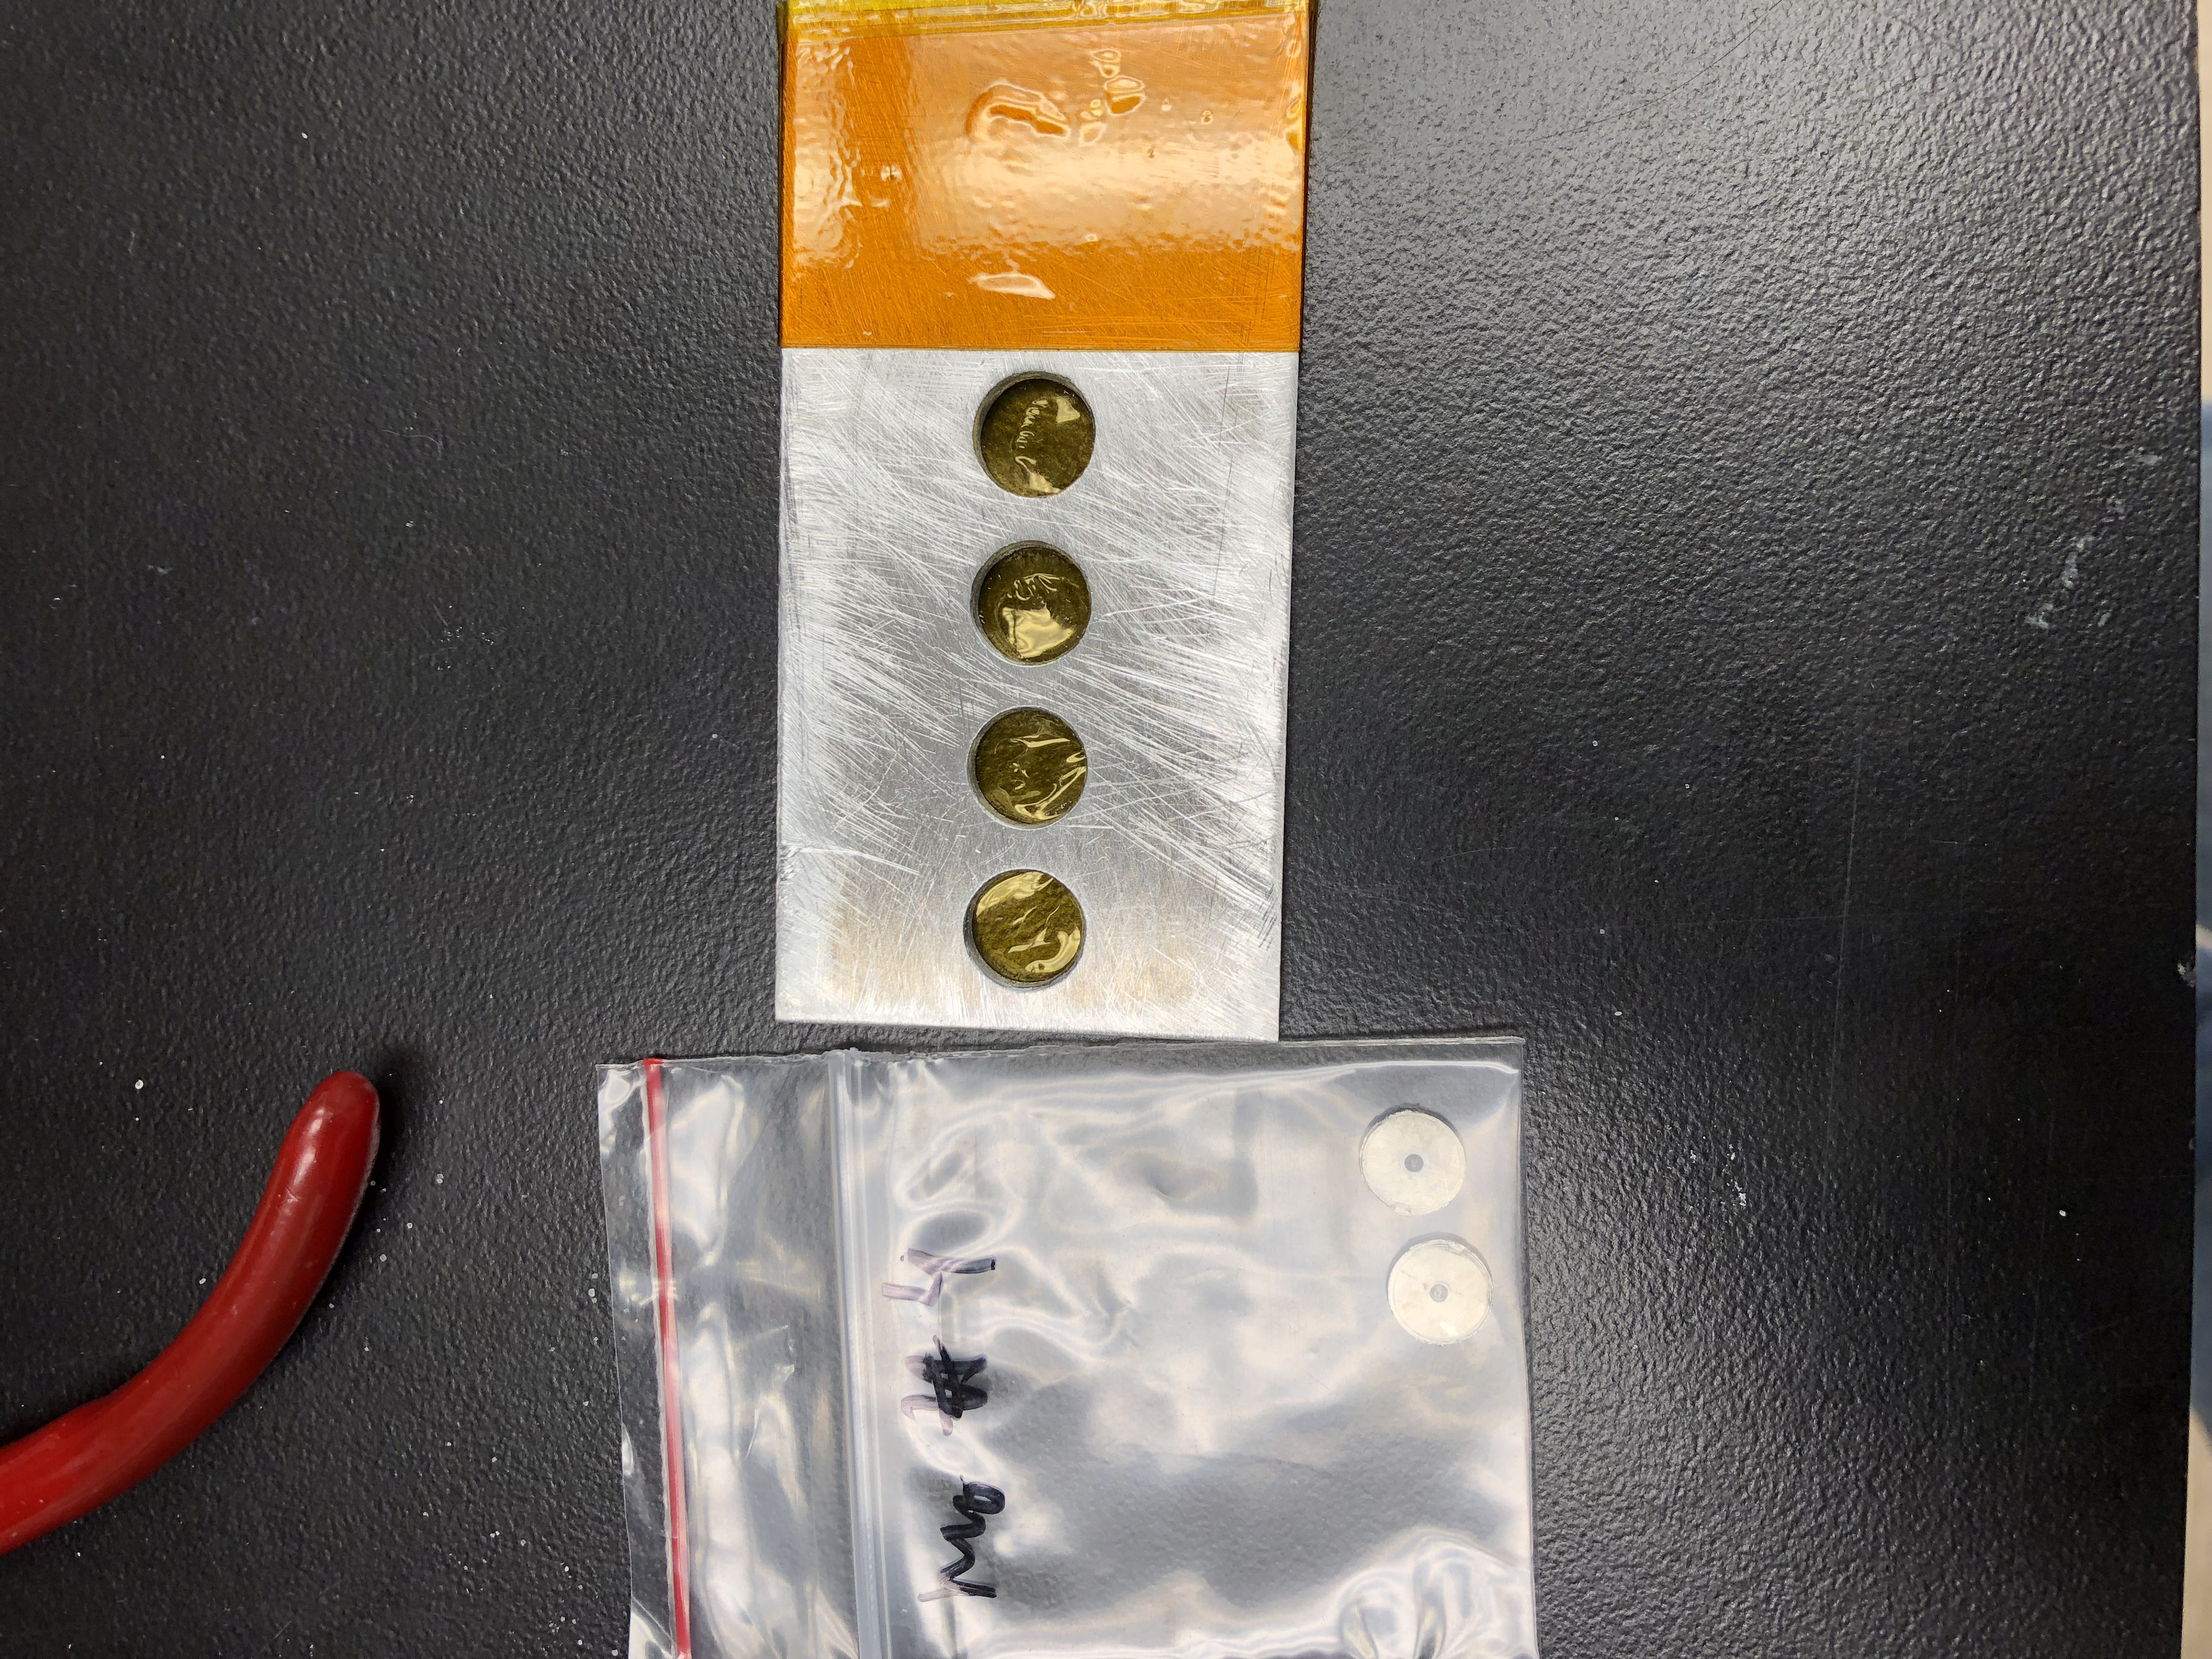
\includegraphics[clip=true,trim=5pt 1000pt 10pt 900pt,width=0.75\columnwidth,angle=90]{./figures/IMG_8840.JPG}
%  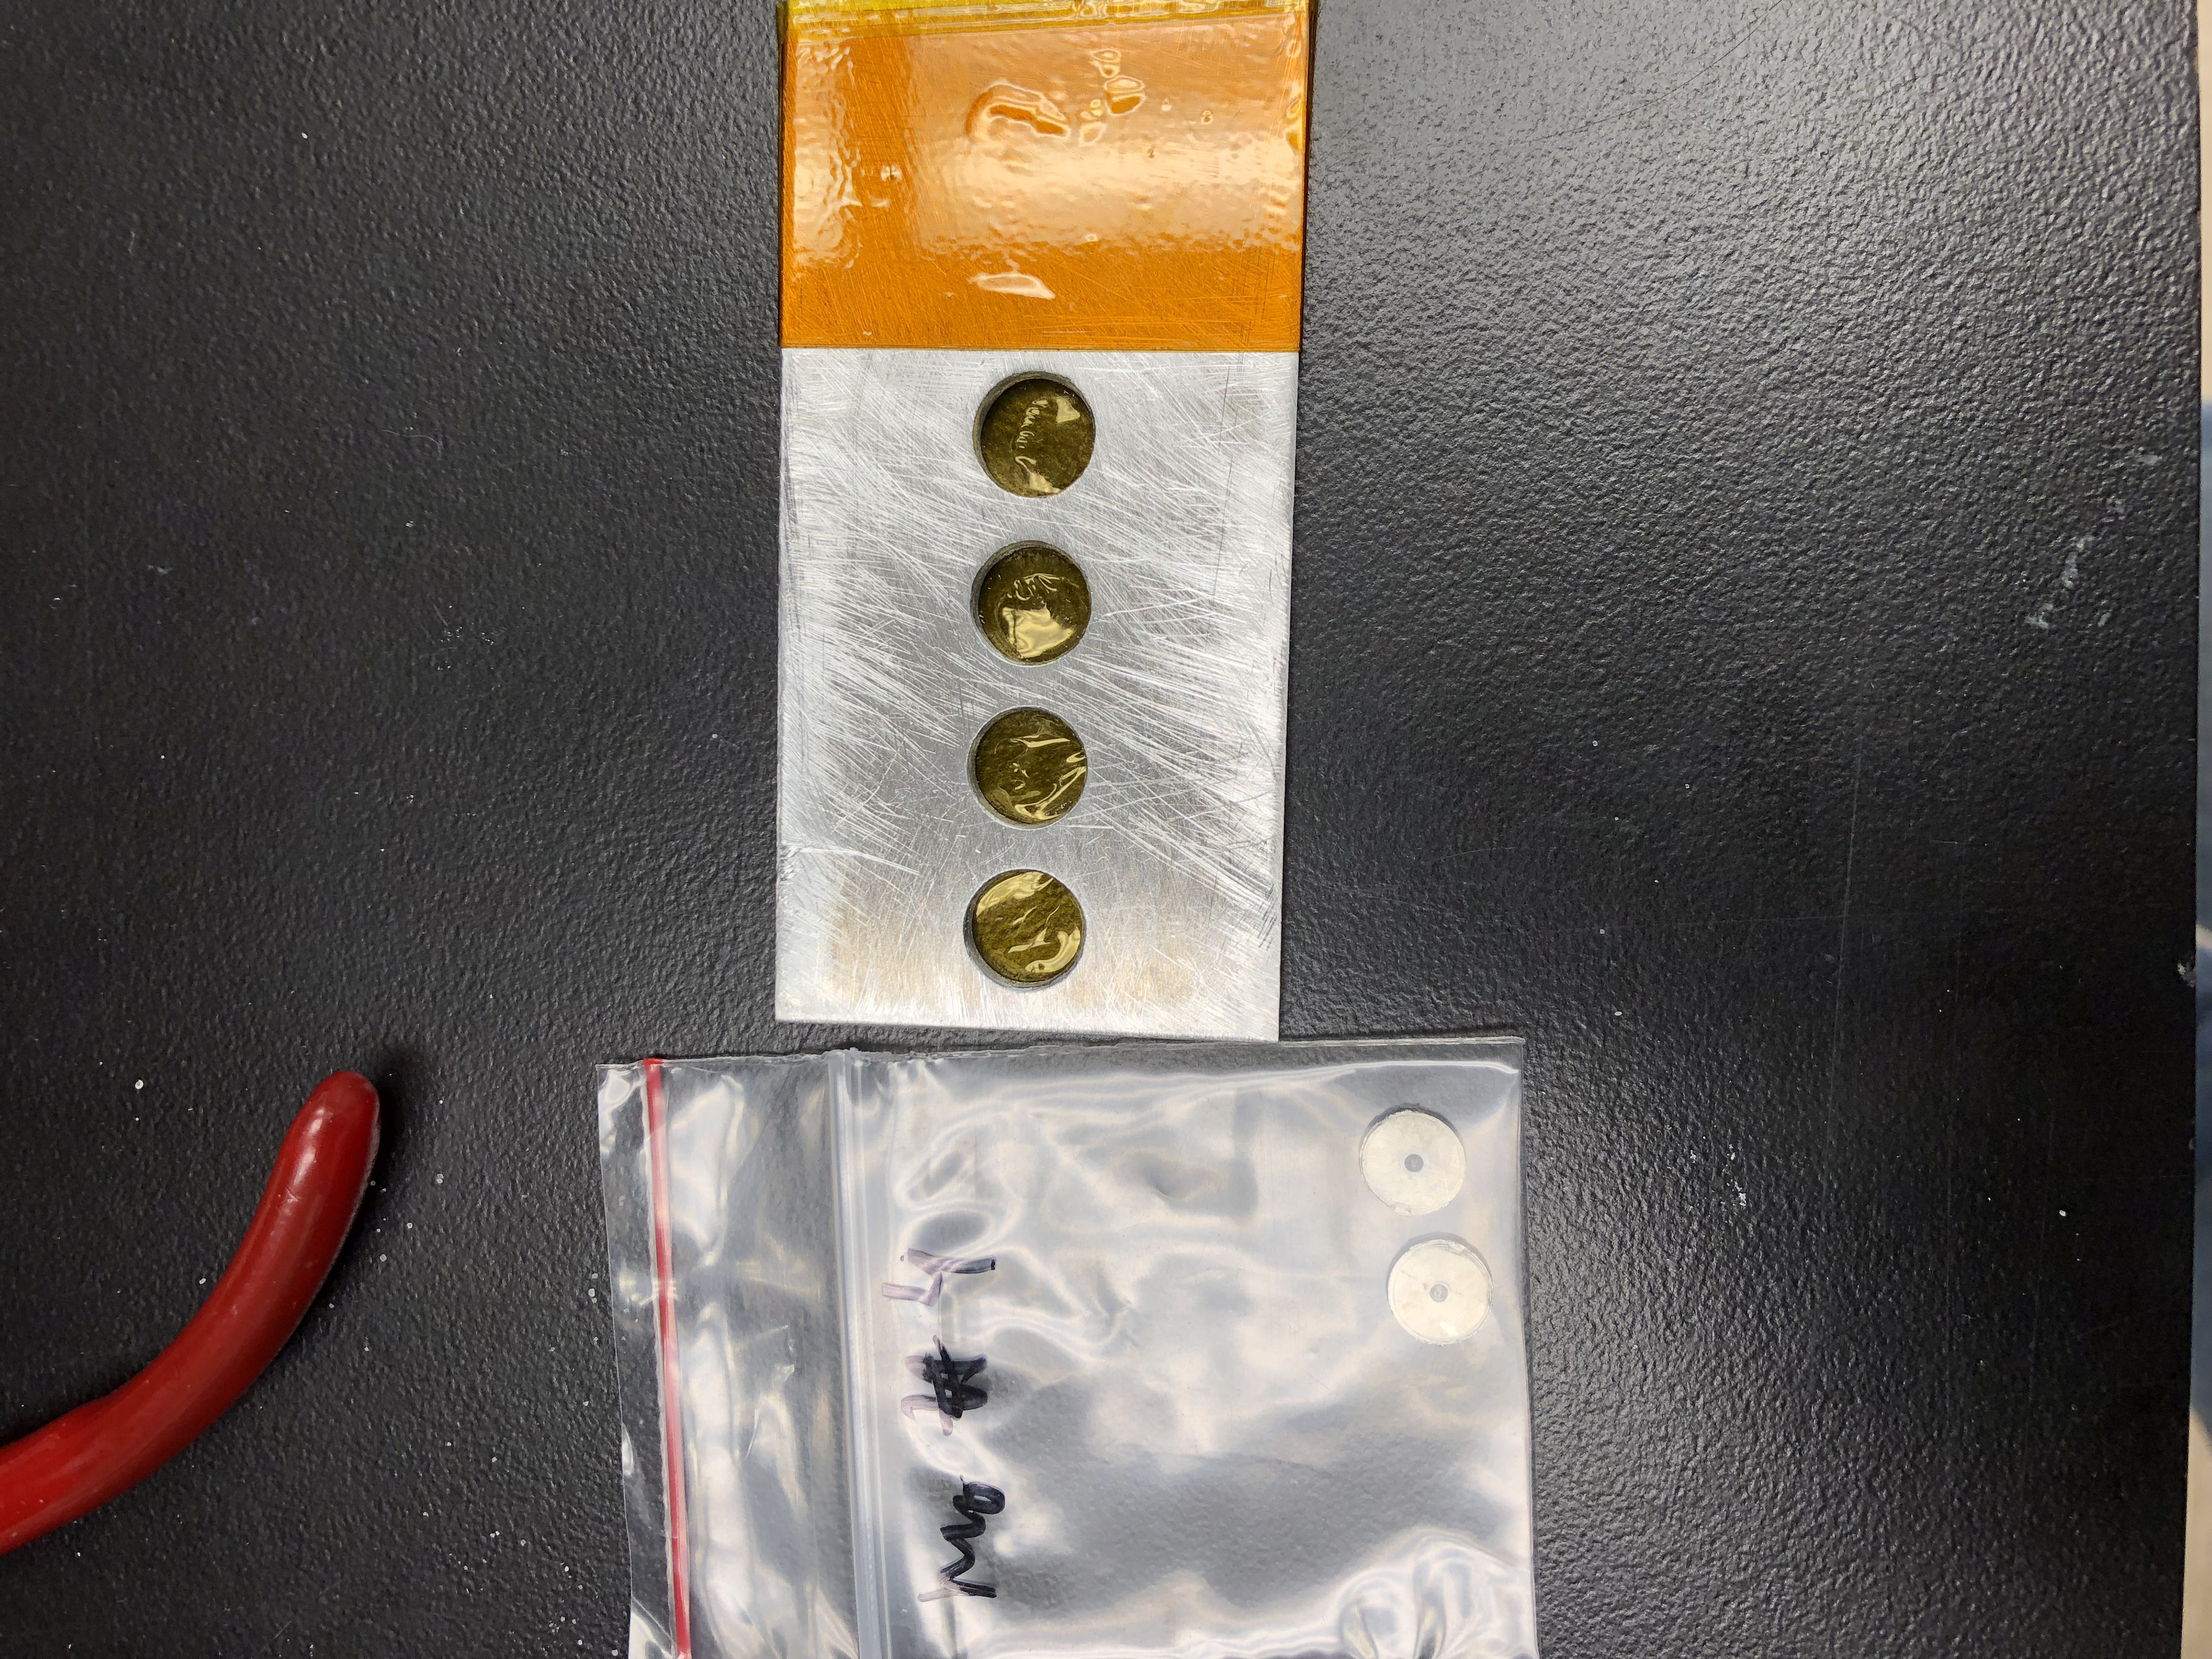
\includegraphics[width=0.75\columnwidth,angle=270]{./figures/IMG_8840.JPG}
 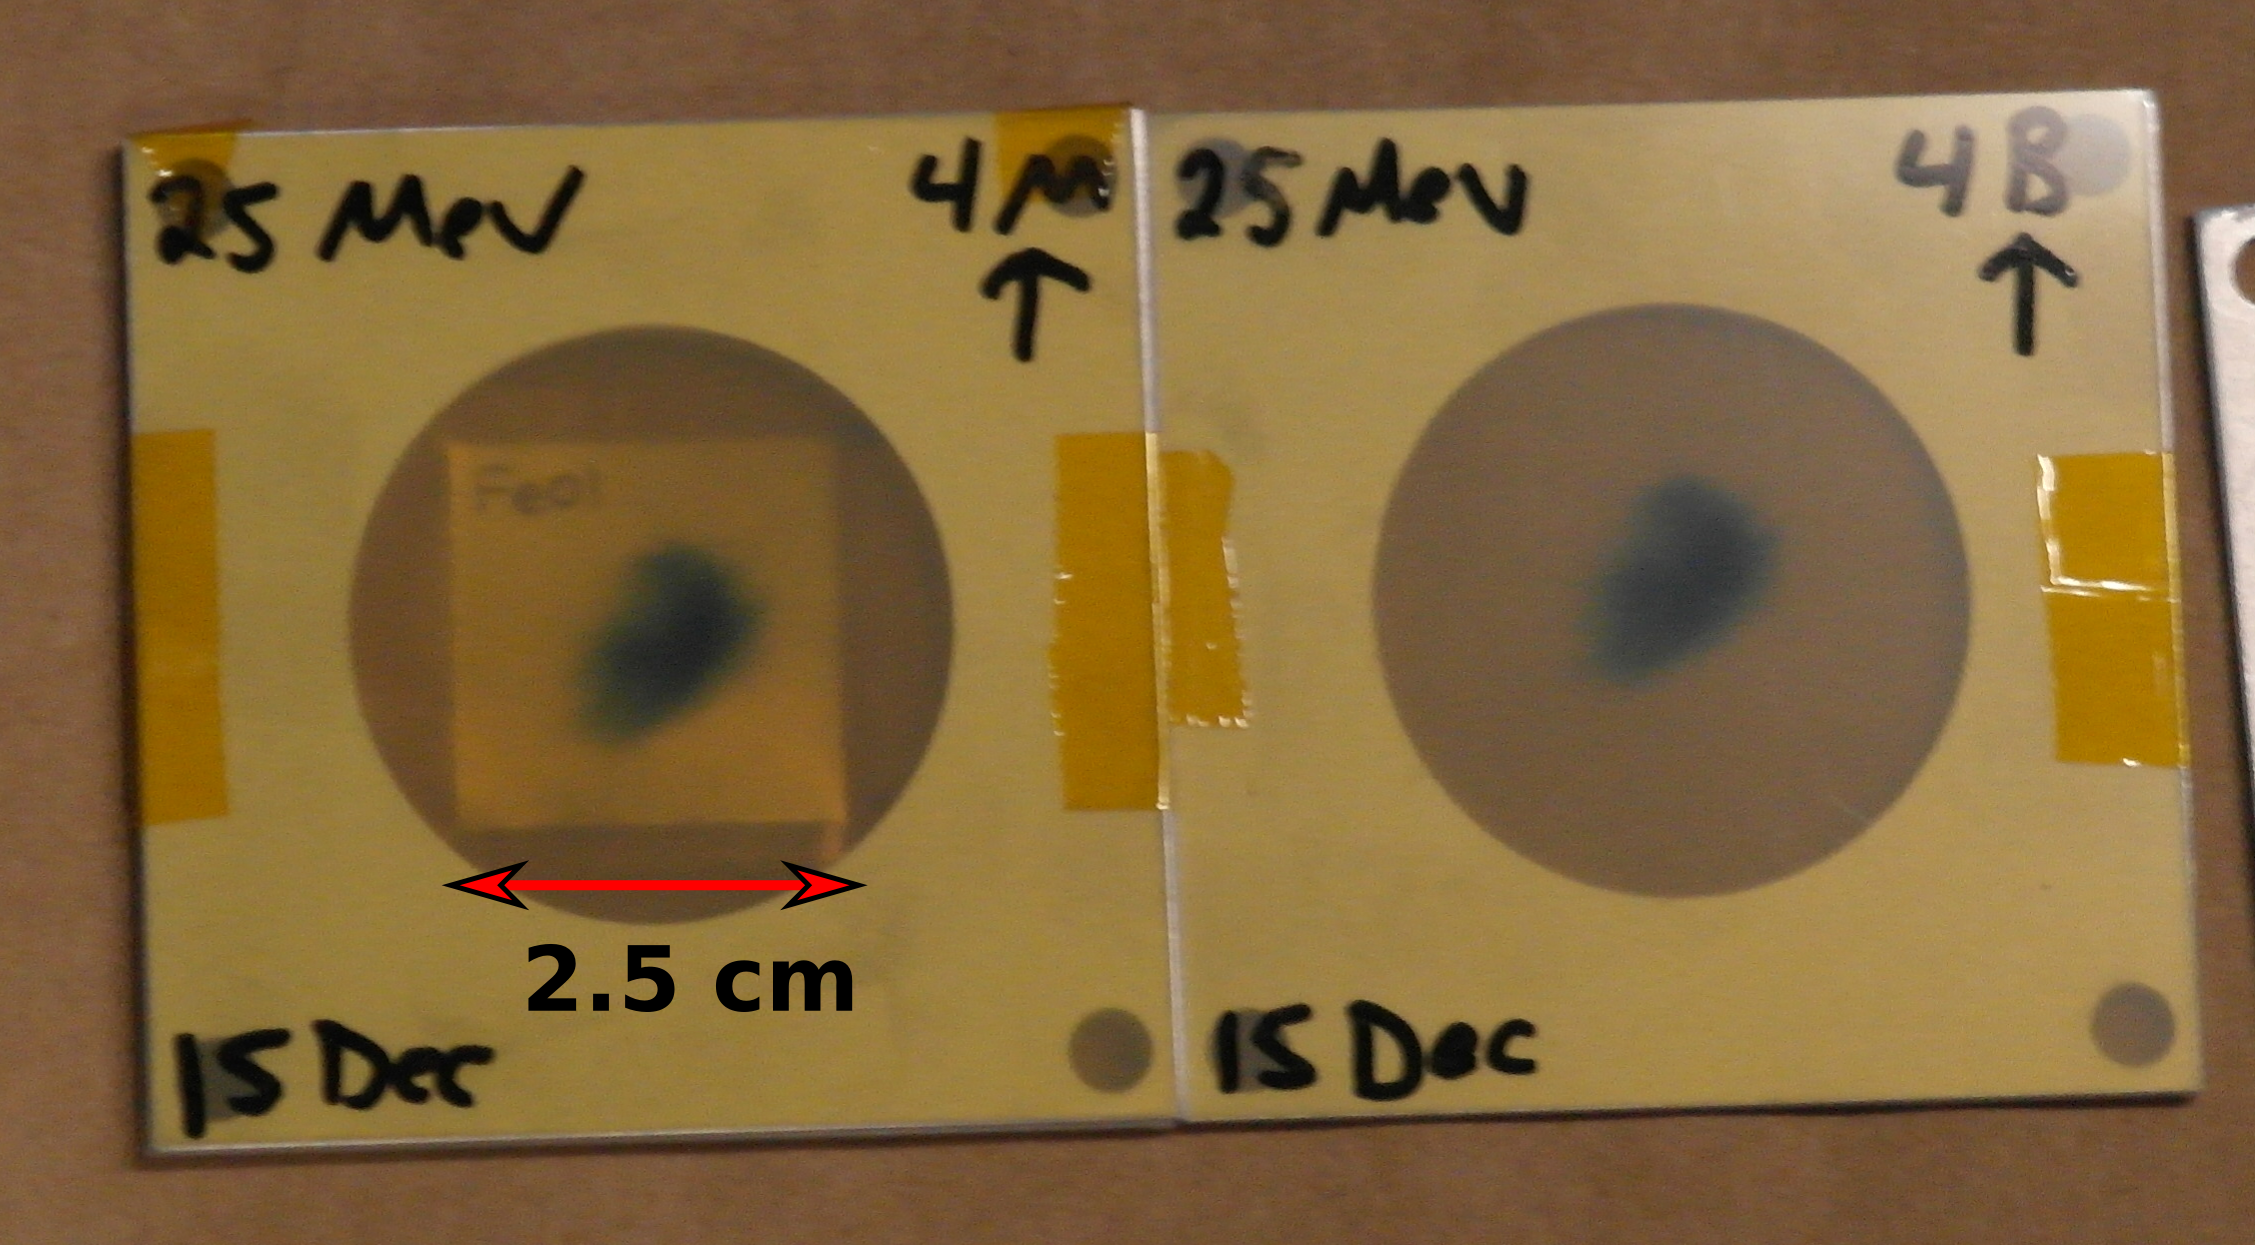
\includegraphics[width=0.75\columnwidth]{./figures/25MeV_optics_films.png}
 % IMG_8840.JPG: 4032x3024 pixel, 72dpi, 142.24x106.68 cm, bb=0 0 4032 3024
 \caption{Final beam spot profile for the 25\,MeV LBNL Fe(p.x) measurement. The  proton beam is confirmed to be centered on the target position, and is focused to underfill the 25$\times$25\,mm target foils.}
 \label{fig:fe25_preexp_beam_spot}
\end{figure}

\begin{figure}
 \centering
%                                l   b      r    top
%  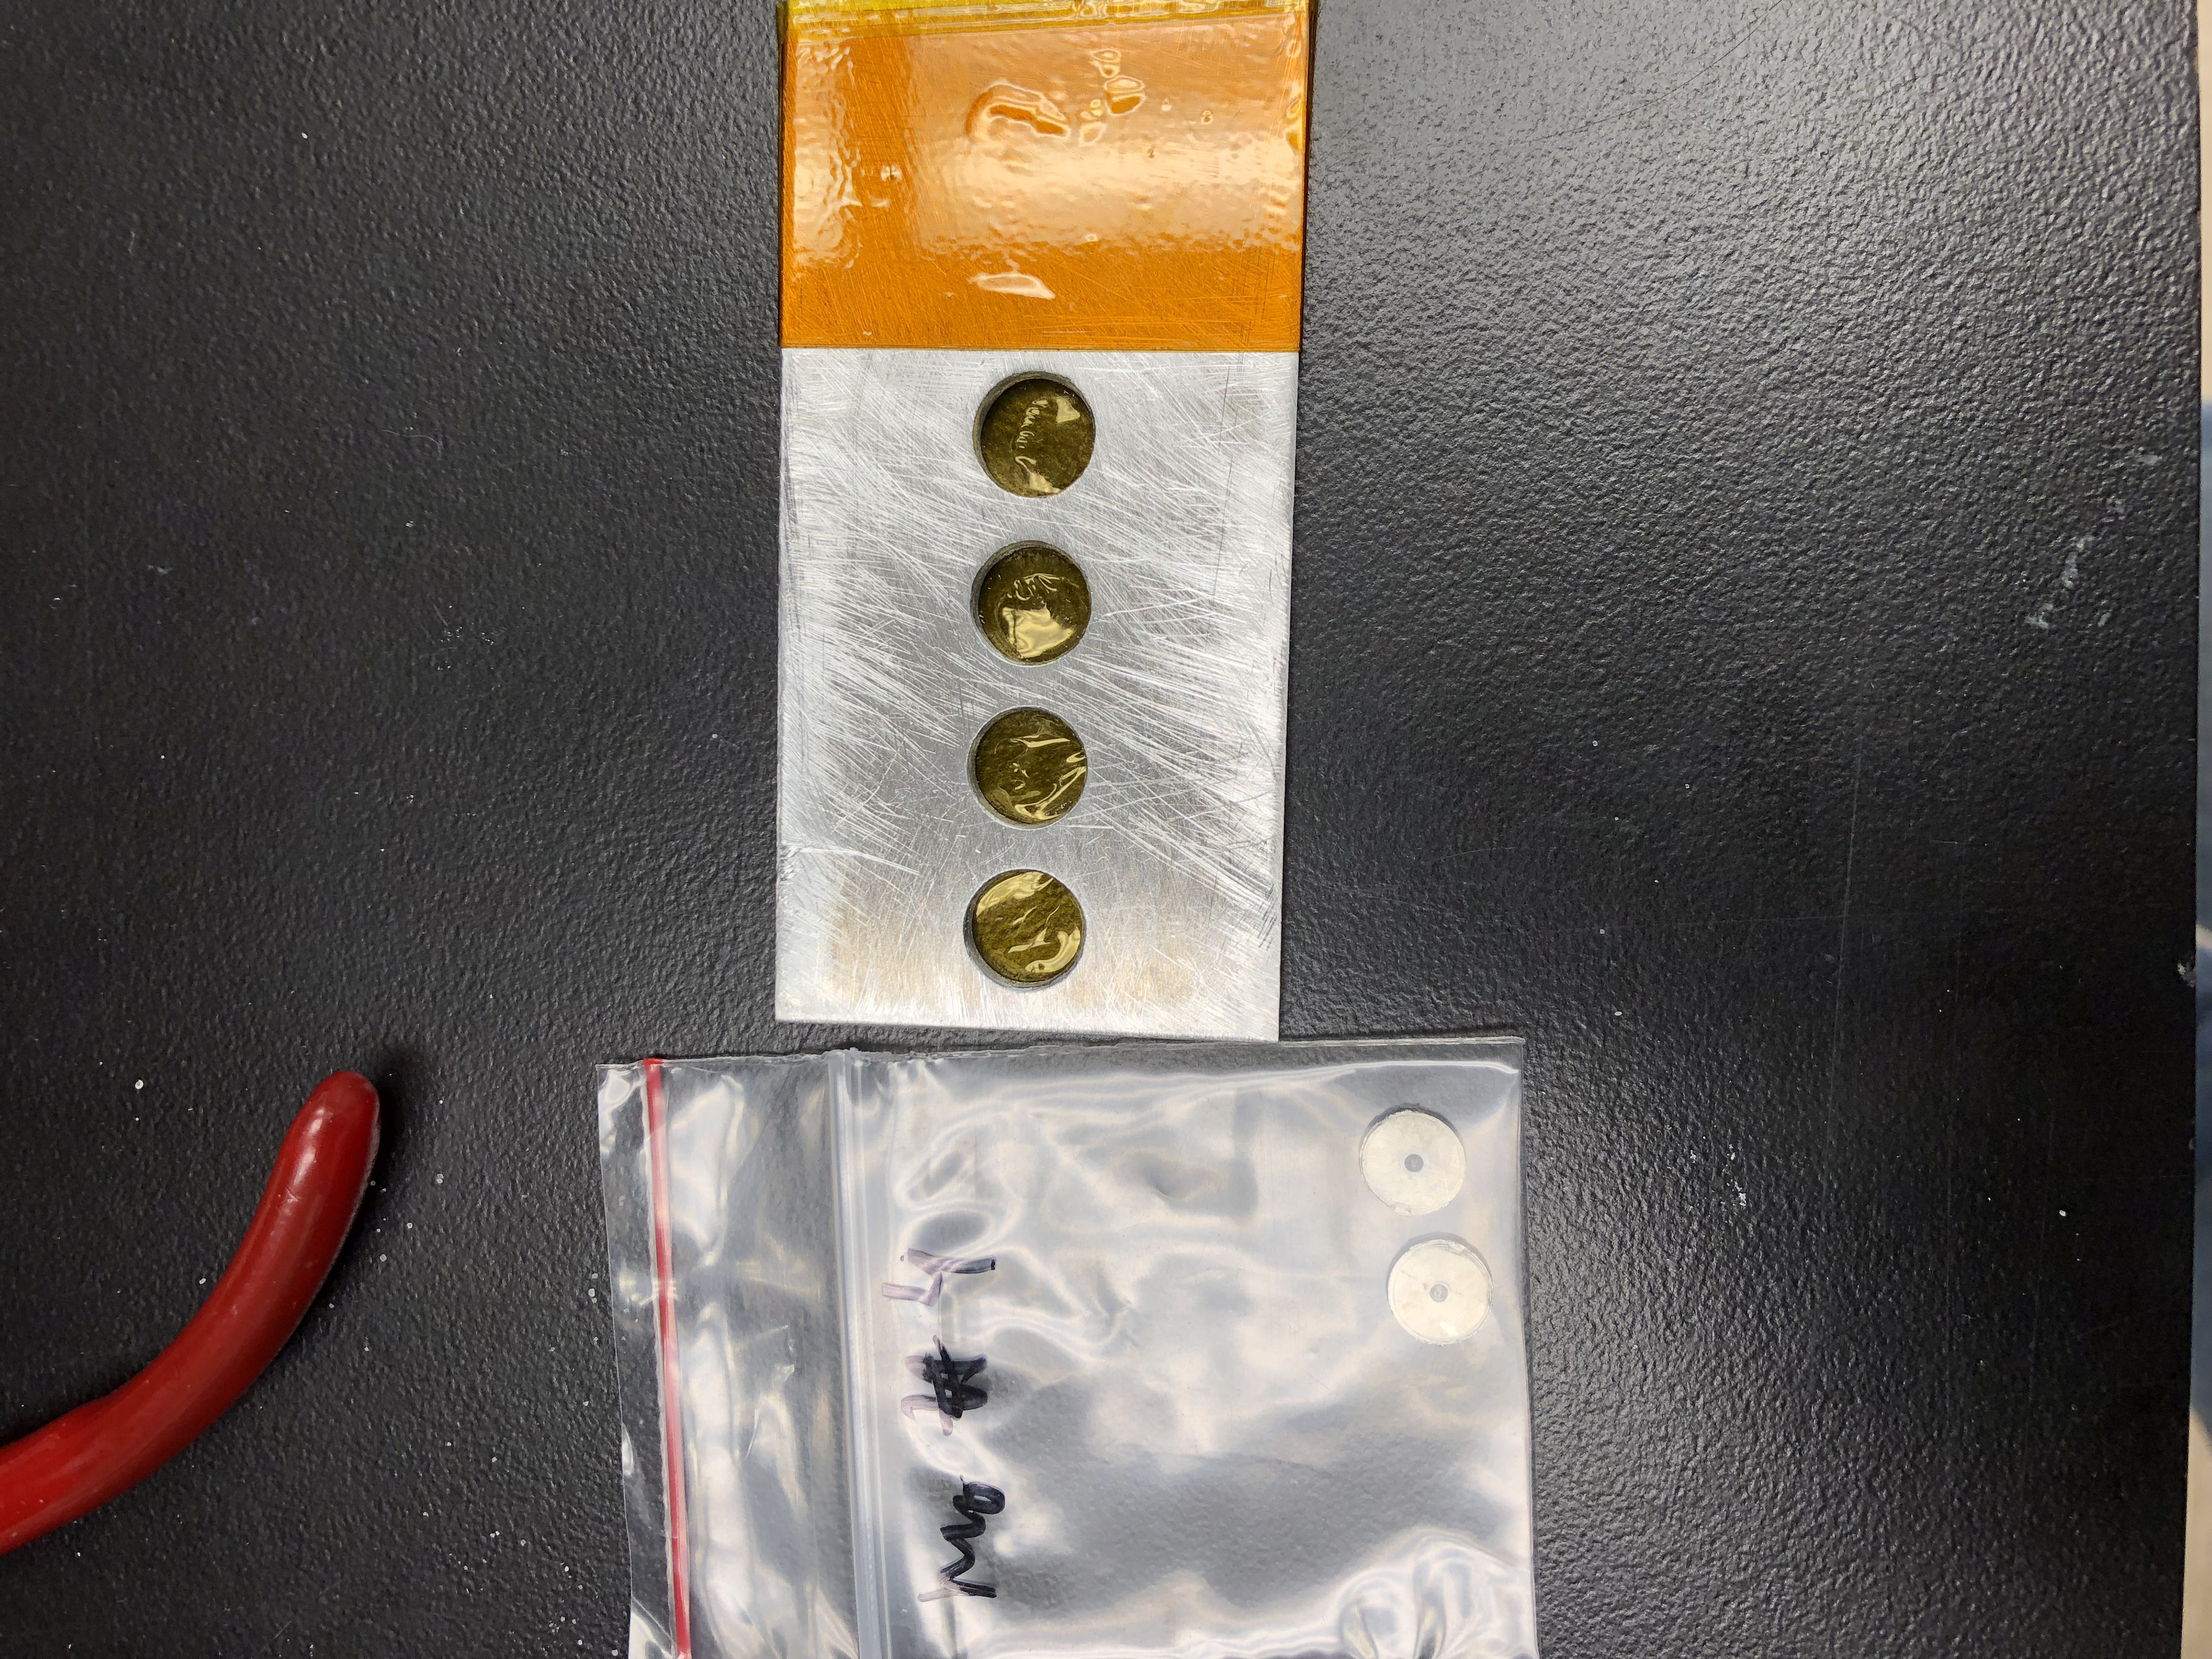
\includegraphics[clip=true,trim=5pt 1000pt 10pt 900pt,width=0.75\columnwidth,angle=90]{./figures/IMG_8840.JPG}
%  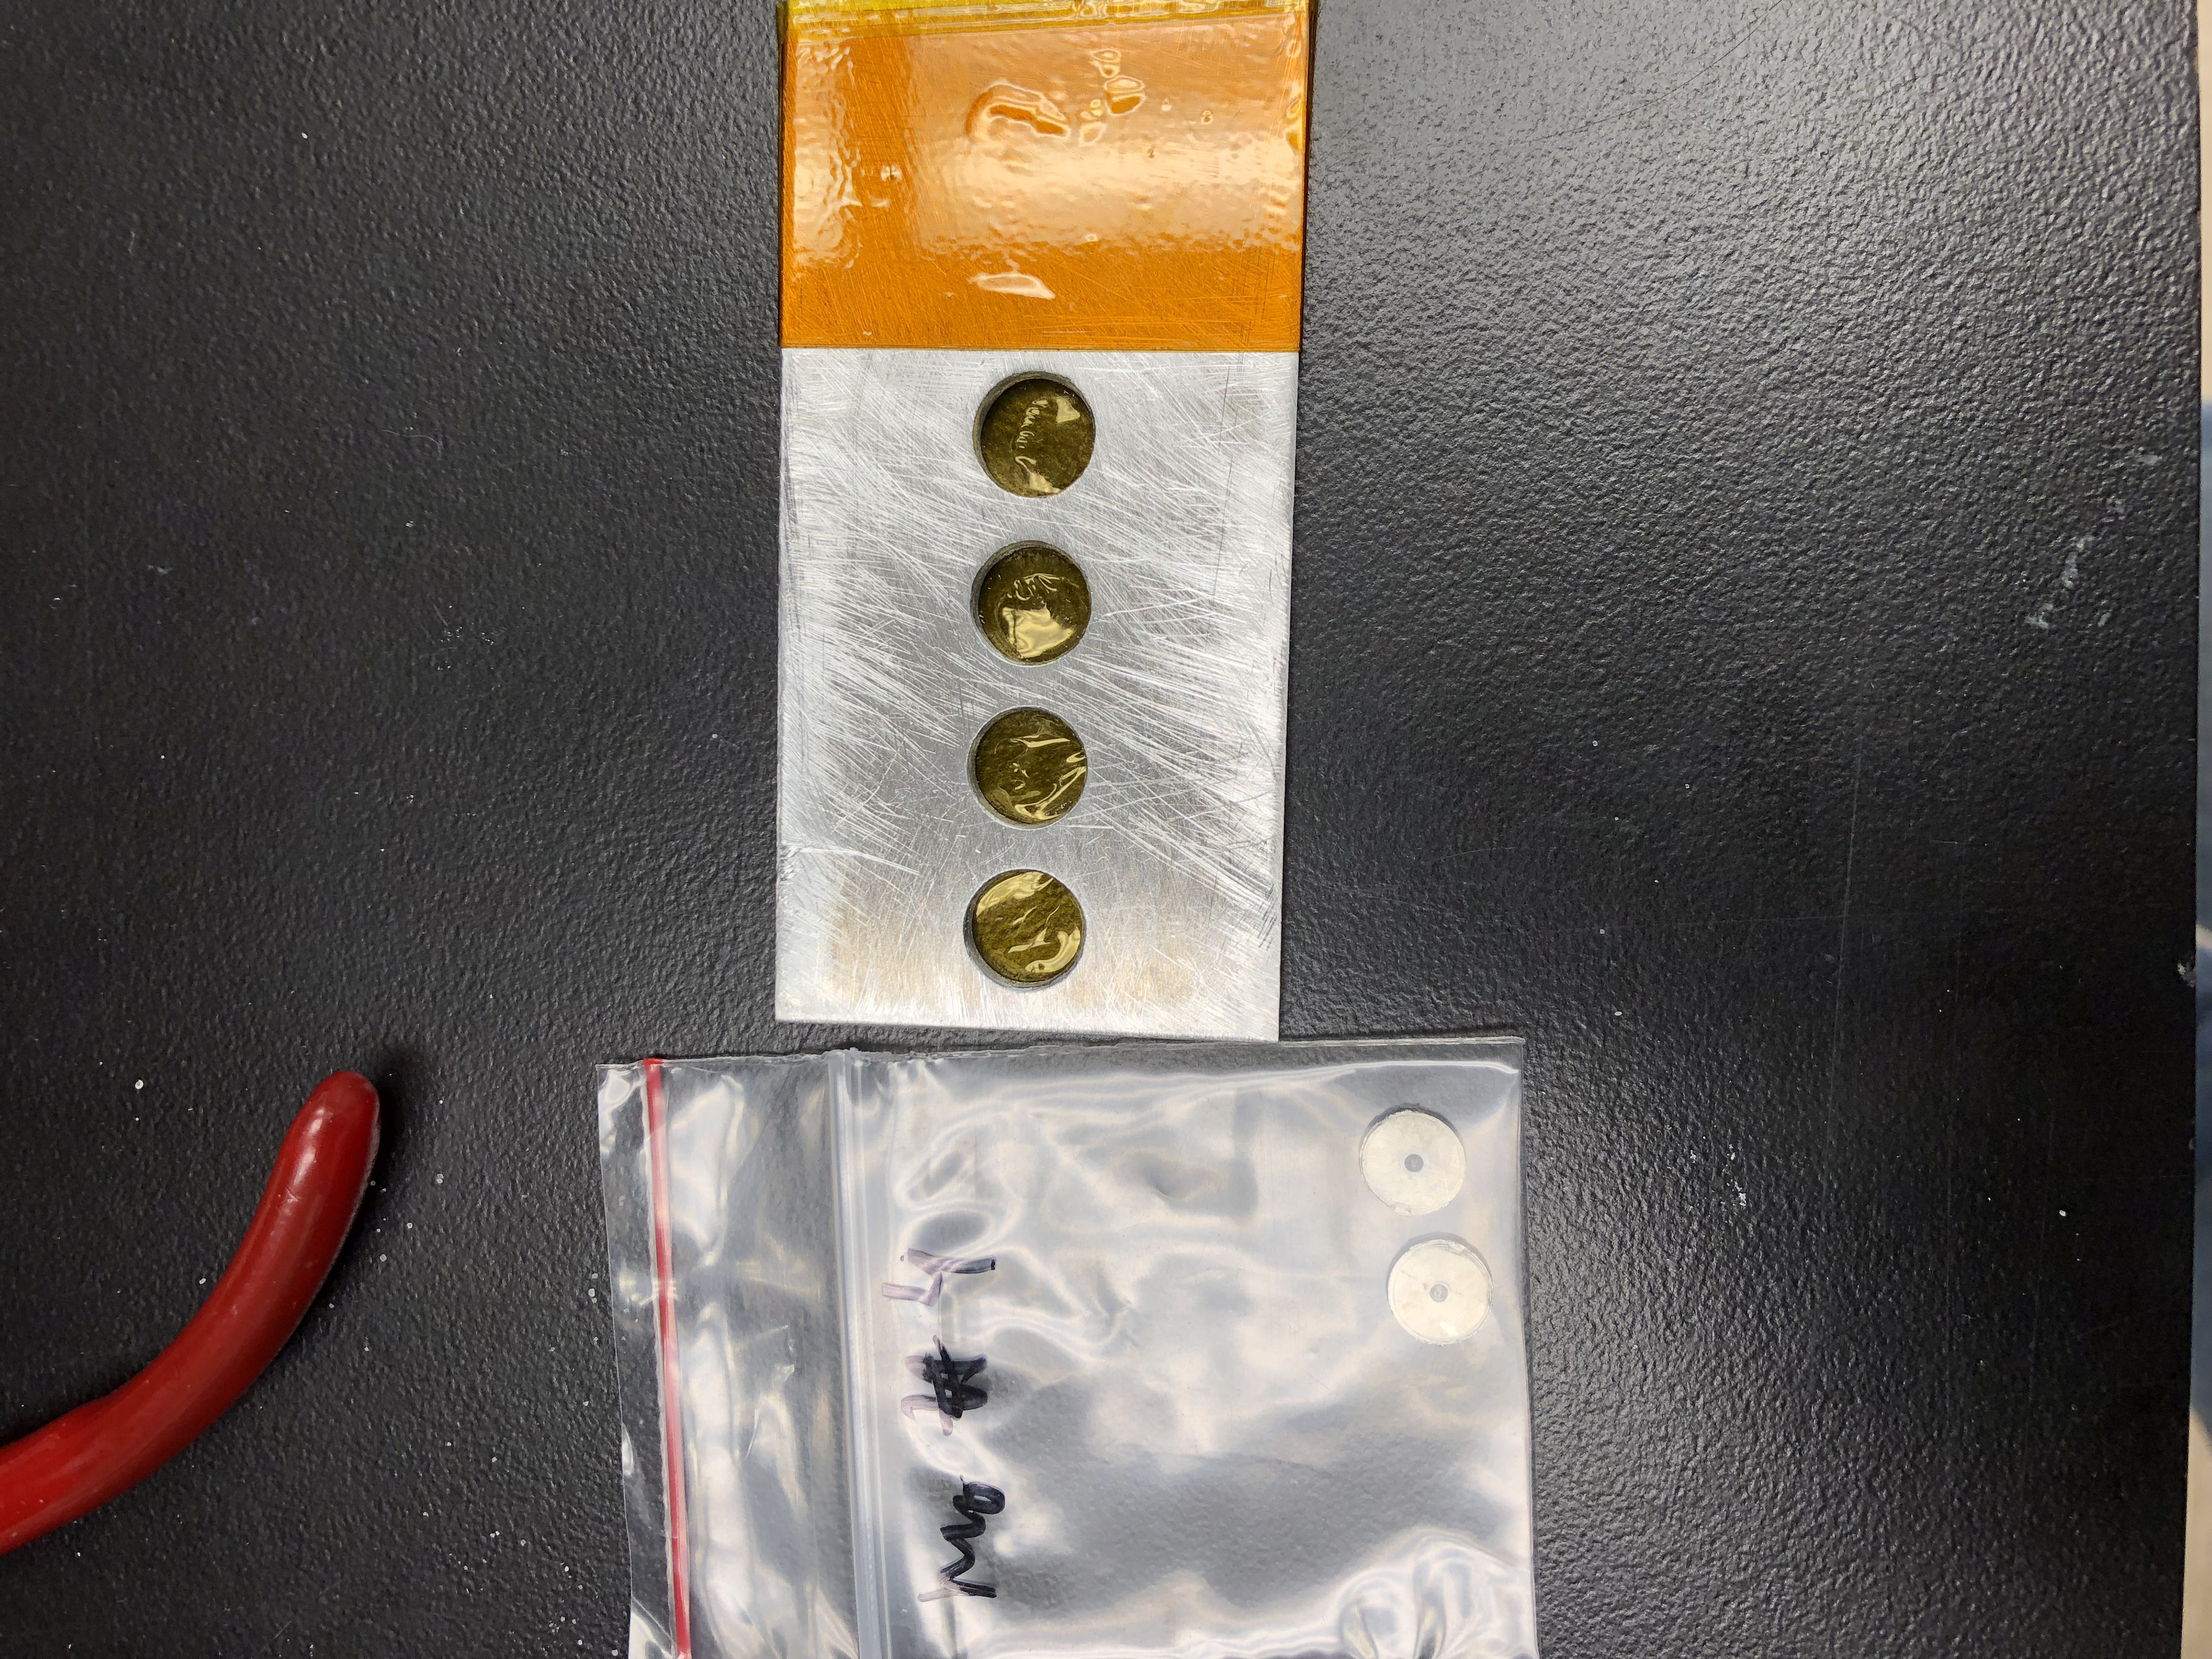
\includegraphics[width=0.75\columnwidth,angle=270]{./figures/IMG_8840.JPG}
 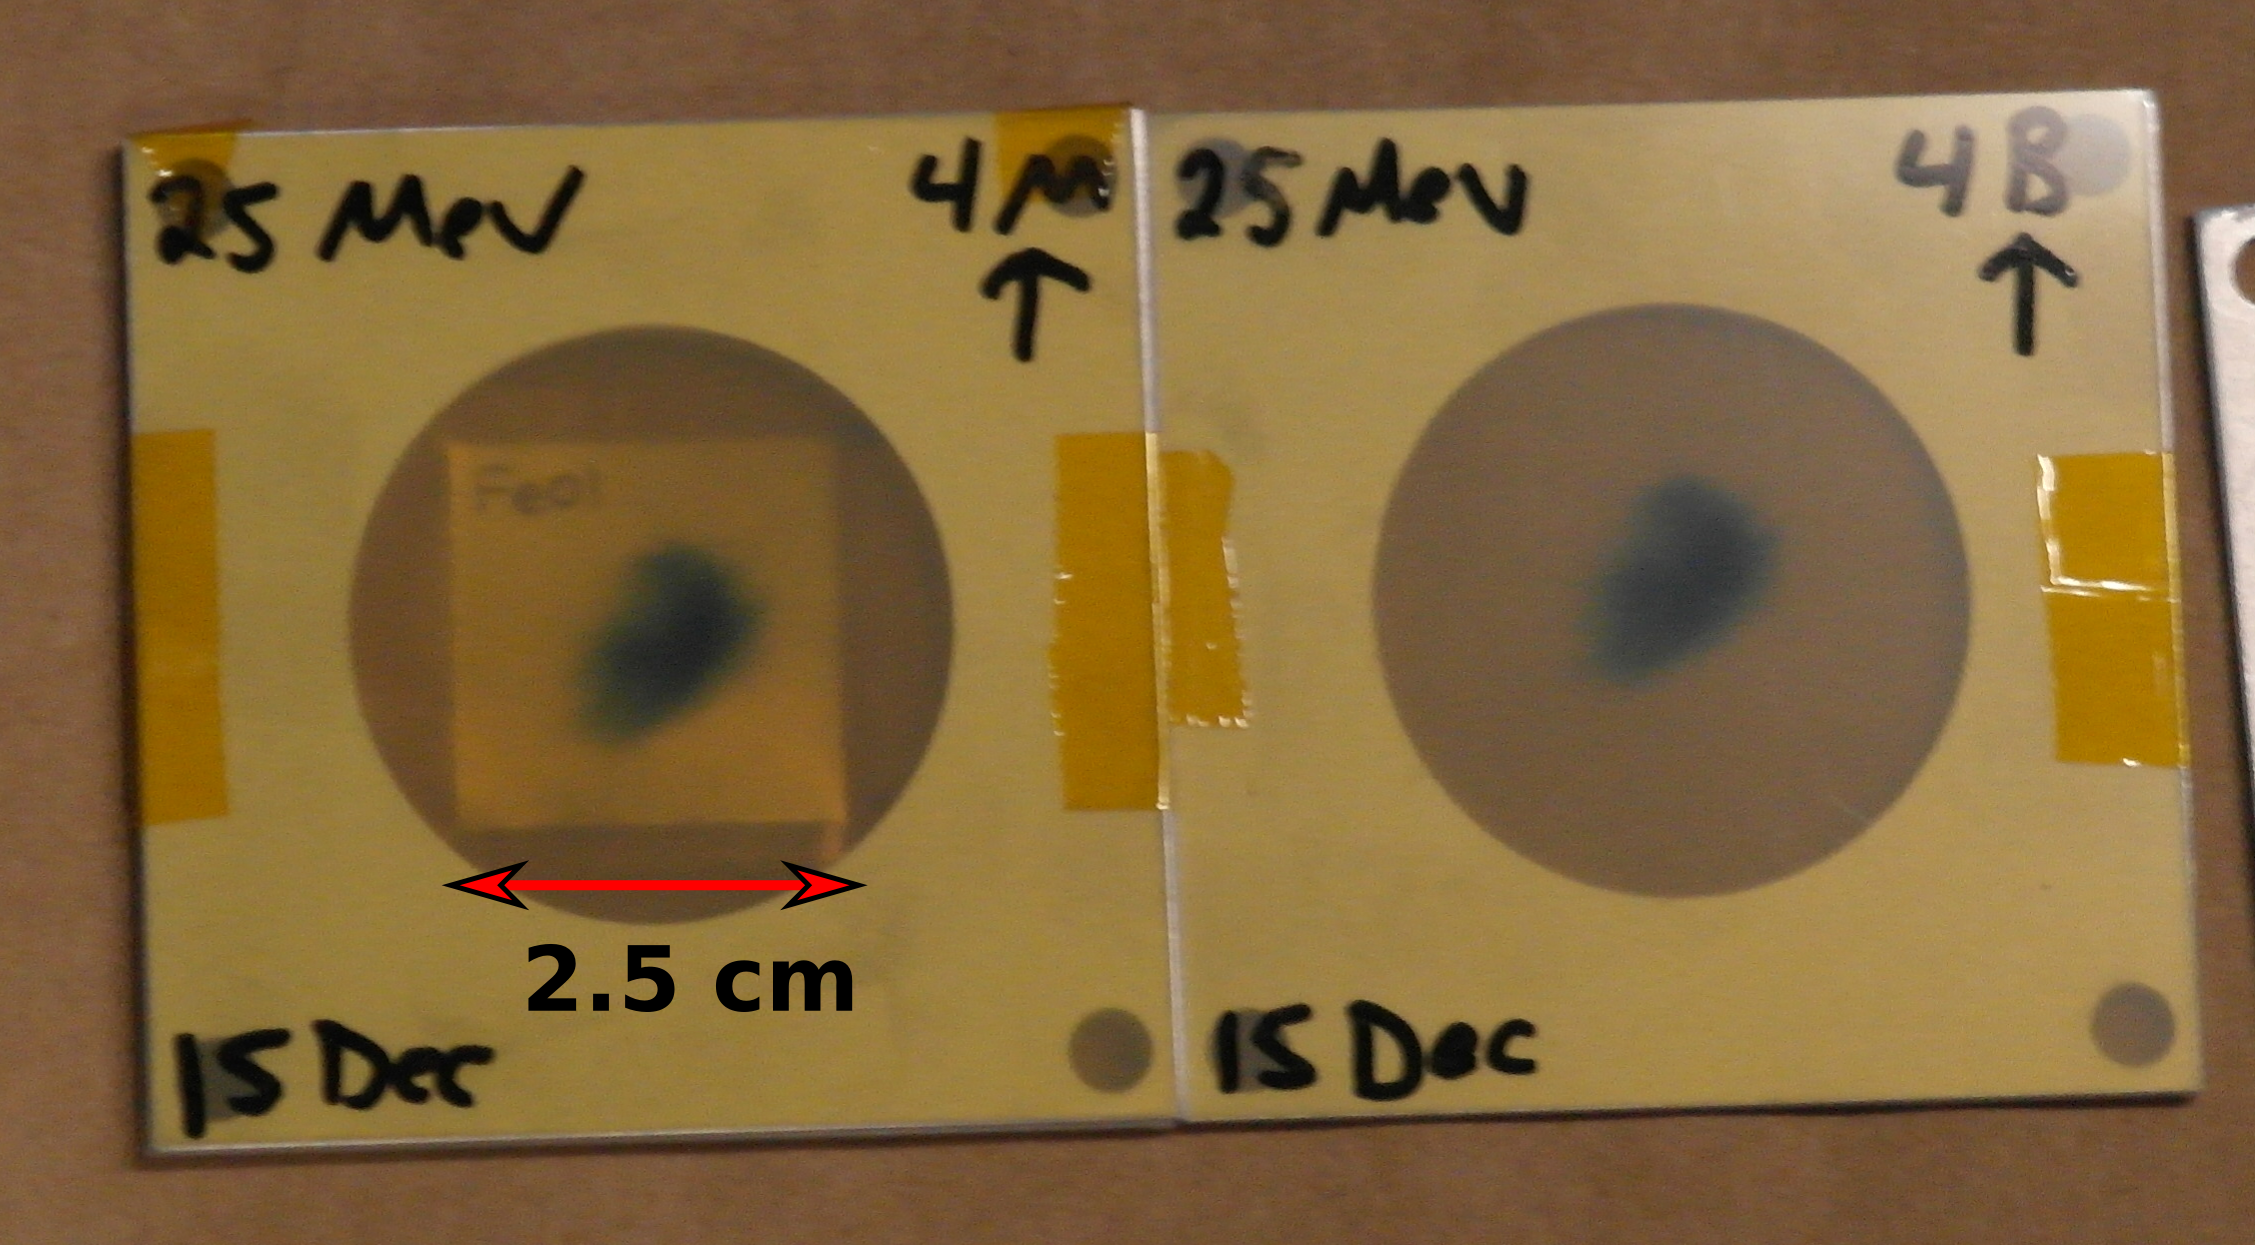
\includegraphics[width=0.75\columnwidth]{./figures/25MeV_optics_films.png}
 % IMG_8840.JPG: 4032x3024 pixel, 72dpi, 142.24x106.68 cm, bb=0 0 4032 3024
 \caption{\textred{Update this figure!!!} Final beam spot profile for the 55\,MeV LBNL Fe(p.x) measurement. The  proton beam is confirmed to be centered on the target position, and is focused to underfill the 25$\times$25\,mm target foils.}
 \label{fig:fe55_preexp_beam_spot}
\end{figure}





These films are useful for determining the beam profile incident upon the front of each stack.
However, the beam broadens as it traverses the target stack, with large-angle deflections (primarily in the aluminum degraders) from scattering of the beam.
To image the actual beam profile incident upon the first foil in the stack (Fe-01 and Fe-08), a 316 stainless steel foil (SS-3 and SS-5) is inserted upstream of Fe-01 and Fe-08, for the 55 and 25\,MeV stacks, respectively, to serve as a beam profile monitor for the activation foils.
Likewise, another stainless steel profile monitor (SS-4 and SS-6) is inserted downstream of the last foil in the stack (H-02 and Cu-20).
These stainless steel monitors are cut to the same length and width as the aluminum frames used for mounting foils, and are characterized in \autoref{tab:fe_stack_table}.



% \textred{Update the type of film used at IPF, here and in the paper!!!}


As described in \autoref{sec:target_design_fe}, decay radiation emitted from the activated stainless steel foils were used to develop radiochromic film (Gafchromic EBT3), revealing the spatial profile of the beam entering and exiting the stack.
% Radiochromic films, such as Gafchromic EBT, come in multiple varieties, depending on the   dose range and the type of ionizing radiation desired to provide sensitivity to. 
% In general, such films are commonly self-developing, containing a radiation-sensitive organic polymer dye as the active layer.
% This dye, much like the polyethylene beam profile monitors, is damaged by ionizing radiation, with multiple free radicals initiated in the process.
% These free radicals result in cross-linking, breaking of double bonds, and fragmentation of the dye polymer, which causes the damaged dye to undergo a large visible change in  color.
% The intensity of this color change is often proportional to the dose received by the film, and is preferred to be energy-independent \cite{Azam1998}.
% Many such films are sensitive to prolonged UV exposure, and will slowly develop if not kept in a  cool, dark environment, leading to systematic errors in observed dose.
% The thin dye layer in most films is extremely sensitive, so care must be taken to avoid bending or deforming, which can make them insensitive to development when irradiated.
% % Following exposure, the film may be scanned 
% For reference, the Gafchromic EBT film used in this work is comprised of a pair of 25\,\mmicro m active layers containing the radiation-sensitive EBT emulsion dye, separated by a 3\,\mmicro m surface layer and sandwiched in between a pair of 97\,\mmicro m layers of clear polyester, acting as a supportive and protective backing. 
% 
% 
% 
% 
% 
% 
% %  Move these first two commented sentences into PhD thesis.
% % 
% % % % 
% % An accurate integrated proton current is one of the most important factors in performing high-fidelity cross section measurements.
% % At the time of this work, the nondestructive beam current monitors in the LANSCE-IPF beamline had a  resolution of 100 nAh.
% % For a low-current irradiation such as this work, where a nominal fluence of 200 nAh is desired, additional fluence sensitivity is thus needed to accurately normalize quantified EoB activities into cross sections.
% 
The radiochromic films developed by the 55\,MeV stack's SS-3 and SS-4 stainless steel beam profile monitors are seen in \autoref{fig:gafchromic_fe}.
In addition, extra \textred{aluminum} monitor foils mounted on  aluminum frames are superimposed behind each film.
It is clear from the upstream (SS-3) film that the proton beam profile was consistent with that seen in the final pre-irradiation beam spot check of  \autoref{fig:fe55_preexp_beam_spot}.
The downstream (SS-4) film  reveals that the beam was not completely attenuated,  
% in the target stack
and clearly displays the  broadening expected due to scattering in the target stack. 
More importantly, the beam profiles in both films appears to be completely contained within the 25$\times$25\,mm activation foils, including the beam envelope.
As discussed previously in \autoref{sec:nb_profile_measurements}, this confirms that the activation foils were exposed to  the total beam current.


% If the beam were to be misaligned on the foils, or were to have sufficiently broadened such that it greatly overfilled the foils, the activation foils would be exposed to only a fraction of the total beam current.
% If  fluence measurements are purely taken from an external  current monitor (such as an inductive pickup upstream of a target, or an electrically-isolated target in a Faraday cup), the  fraction of current which misses the foils will not be detected.
% This leads to reporting a false, larger  fluence, which will cause all cross sections to be erroneously reported with a reduced magnitude.
% Thus, it is for this  reason that having monitor foils at each energy position builds confidence in reported cross sections, as they serve to screen for systematic errors such as this.
% However, profile monitors play a vital role in the detection of lost beam fluence when monitor foils are unavailable. 
% Additionally, 







% Since the color change developed by irradiation is proportional to the dose deposited in the film, the optical density of the film may be used to measure dose.
% In clinical external-beam radiation therapy, these films are commonly used in quality assurance  to map and verify  the dose contours for therapeutic gamma-ray fields.
% However, the dose sensitivity of these films is often greater than the ability to be visually distinguished beyond simple qualitative inspection.
% As a result, following exposure, the film may be digitized using any flatbed scanner.
% Image analysis may be thus used to measure the optical density profile as a surrogate for dose or beam intensity profiles.
% The optical density is often fit to a curve of the form
% \begin{equation}
% d_x\pp{D} = a + \dfrac{b}{D-c}
% \end{equation}
% where $d_x\pp{D}$ is the optical density of exposed radiochromic film in scanner color channel $x$ at dose $D$, and $a$, $b$, and $c$ are calibration parameters.
% Using a standard irradiation source (commonly a collimated \ce{^{60}Co} source), a calibration curve can thus be measured to convert optical density into an absolute dose.
% This is most common in clinical and quality assurance applications.
% In addition, modern radiochromic films are often designed such that the characteristic exposure curve for the active layer dye differs between the red, green, and blue color channels, offering even further enhanced sensitivity to dose \cite{bushberg2011essential,Andre2011,David2012}.





% However, for cases where an absolute dose is not necessary, the optical density can still be used for a qualitative measure of relative beam intensity, or relative dose.
Using the image analysis code  ImageJ-2.0.0,  profiles of the total optical density were extracted for both the SS-3 and SS-4 radiochromic films \cite{Rueden2017}.
These are seen in \autoref{fig:gafchromic_fe_profiles}, as relative beam intensity profiles along the major and minor axis of each film.
As seen visually, for both axes, the peak beam intensity drops from SS-3 to SS-4, as the proton fluence is clearly broadened by scattering reactions in the target stack.
% As seen visually, there is a clear broadening of the beam spot in the rear of the target stack.
Along the major (\enquote{horizontal}) axis, the FWHM of the beam profile broadens from \textred{0.679\,cm to 1.039\,cm}, and along the minor (\enquote{vertical}) axis, the FWHM of the beam profile broadens from \textred{0.453\,cm to 0.902\,cm.}
In addition, the centroid position of the minor axis appears to shift by approximately \textred{0.19\,cm} between the front and rear of the stack. 
The measured beam profiles were fit using a Gaussian model with linear background, to aid in comparing the widths of each profile.
The Gaussian model does well to fit the beam profiles overall, though it overestimates the peak height for a given Gaussian width.
This is likely due to the fact that the beam itself has an intrinsic spatial width before any interactions with the target stack; this leads to more broadening of the beam envelope than of its core.

    

% 55\, MeV
% 
\begin{figure}
    \centering
    \subfloat{
        \centering
%         \includegraphics[width=\columnwidth]{./figures/Capture.PNG}
        \hspace{-5pt}\subfigimg[width=0.5\textwidth]{a)}{./figures/DOC013119-cropped.pdf}{80}
%         \caption{ Decay curve for the isomeric transition of \ce{^{115m}In}.}
         %         \refstepcounter{subfigure}
         \label{fig:gafchromic_fe_upstream}
   \hspace{-5pt}}%
     \subfloat{
        \centering
%         \includegraphics[width=\columnwidth]{./figures/Capture.PNG}
%         \includegraphics[scale=0.6]{./figures/391keV_curve2.png}
        \subfigimg[width=0.5\textwidth]{b)}{./figures/DOC013118-cropped.pdf}{80}
%         \caption{ Decay curve for the isomeric transition of \ce{^{113m}In}.}
         %         \refstepcounter{subfigure}
         \label{fig:gafchromic_fe_downstream}
   \hspace{-5pt}}%
    \caption{\textred{Update this figure!!!} Radiochromic films for the 55\,MeV LBNL Fe(p,x) measurement, developed by the stainless steel beam profile monitors in (a) the front of the stack (SS-3) and (b) the rear of the stack (SS-4). An unused \textred{Al} monitor foils is aligned behind each film, confirming that both the beam core and envelope underfilled the activation foils.}
     \label{fig:gafchromic_fe}
\end{figure}




\begin{figure}
    \centering
    \subfloat{
        \centering
%         \includegraphics[width=\textwidth]{./figures/target2.png}
        \subfigimg[width=0.496\textwidth]{a)}{./figures/horz_ipf_beam_profile.pdf}{100}
%         \caption{Decay curve for the $\beta^-$ decay of \ce{^{116}In}.}
        %         \refstepcounter{subfigure}
%          \label{fig:54Mn}
%
%         \includegraphics[width=\columnwidth]{./figures/Capture.PNG}
        \subfigimg[width=0.496\textwidth]{b)}{./figures/vert_ipf_beam_profile.pdf}{50}
%         \caption{ Decay curve for the $\beta^+$ decay of \ce{^{64}Cu}.}
%         \refstepcounter{subfigure} 
%         \label{fig:55Co}
   \hspace{-10pt}}%
    \caption{\textred{Update this figure!!!} Relative beam intensity profiles for the radiochromic films seen in \autoref{fig:gafchromic_fe}. The intensity profiles were analyzed using ImageJ along (a) the major axis and (b) minor axis of each beam spot. }
     \label{fig:gafchromic_fe_profiles}
\end{figure}




Similar profile measurement results are presented here for the 25\,MeV stack as well.
The radiochromic films developed by the 25\,MeV stack's SS-5 and SS-6 stainless steel beam profile monitors are seen in \autoref{fig:gafchromic_fe_25}.
In addition, extra \textred{aluminum} monitor foils mounted on  aluminum frames are superimposed behind each film.
It is clear from the upstream (SS-5) film that the proton beam profile was consistent with that seen in the final pre-irradiation beam spot check of  \autoref{fig:fe25_preexp_beam_spot}.
However, in a significant departure from the 55\,MeV stack, no exposure is seen in the  downstream (SS-6) film.
This confirms the observation (based on a lack of HPGe-observed activity in the Ti-20 and Cu-20 monitor foils) that the beam was completely attenuated before the end of target stack.
As discussed in \autoref{sec:proton_transport_fe}, this is primarily due to the actual target stack having a greater areal density than estimated during the stack design phase.
The majority of this additional unaccounted areal density arises from the acrylic adhesive in the multiple Kapton tape layers.  
% in the target stack
% and clearly displays the  broadening expected due to scattering in the target stack. 
However,  the beam profile in the upstream film appears to be completely contained within the 25$\times$25\,mm activation foils, including the beam envelope.
This small consolation confirms that the stack received the full entrance fluence, so the validity of the cross sections extracted from this stack still holds.
% As discussed previously in \autoref{sec:nb_profile_measurements}, this confirms that the activation foils were exposed to  the total beam current.
Profiles of the total optical density were extracted for  the SS-5 radiochromic film,  seen in \autoref{fig:gafchromic_fe_profiles_25}, as relative beam intensity profiles along the major and minor axis of the film.
% For both axes, the peak beam intensity drops from SS-3 to SS-14, as the proton fluence is clearly broadened by scattering reactions in the target stack.
% As seen visually, there is a clear broadening of the beam spot in the rear of the target stack.
While no commentary on the peak intensity and broadening can be provided due to the attenuation of the beam within the stack, the entrance profile may at least be reported.
Along the major (\enquote{horizontal}) axis, the FWHM of the beam is \textred{0.679\,cm}, and along the minor (\enquote{vertical}) axis, the FWHM of the beam profile is \textred{0.453\,cm.}







% 25\, MeV
% 
\begin{figure}
    \centering
    \subfloat{
        \centering
%         \includegraphics[width=\columnwidth]{./figures/Capture.PNG}
        \hspace{-5pt}\subfigimg[width=0.5\textwidth]{a)}{./figures/DOC013119-cropped.pdf}{80}
%         \caption{ Decay curve for the isomeric transition of \ce{^{115m}In}.}
         %         \refstepcounter{subfigure}
         \label{fig:gafchromic_fe_upstream_25}
   \hspace{-5pt}}%
     \subfloat{
        \centering
%         \includegraphics[width=\columnwidth]{./figures/Capture.PNG}
%         \includegraphics[scale=0.6]{./figures/391keV_curve2.png}
        \subfigimg[width=0.5\textwidth]{b)}{./figures/DOC013118-cropped.pdf}{80}
%         \caption{ Decay curve for the isomeric transition of \ce{^{113m}In}.}
         %         \refstepcounter{subfigure}
         \label{fig:gafchromic_fe_downstream_25}
   \hspace{-5pt}}%
    \caption{\textred{Update this figure!!!} Radiochromic films for the 25\,MeV LBNL Fe(p,x) measurement, developed by the stainless steel beam profile monitors in (a) the front of the stack (SS-5) and (b) the rear of the stack (SS-6). An unused \textred{Al} monitor foils is aligned behind each film, confirming that both the beam core and envelope underfilled the activation foils. No exposure is seen in the SS-6 film, as the beam was stopped upstream within the target stack, between Fe-14 and Ti-20.}
     \label{fig:gafchromic_fe_25}
\end{figure}




\begin{figure}
    \centering
    \subfloat{
        \centering
%         \includegraphics[width=\textwidth]{./figures/target2.png}
        \subfigimg[width=0.496\textwidth]{a)}{./figures/horz_ipf_beam_profile.pdf}{100}
%         \caption{Decay curve for the $\beta^-$ decay of \ce{^{116}In}.}
        %         \refstepcounter{subfigure}
%          \label{fig:54Mn}
%
%         \includegraphics[width=\columnwidth]{./figures/Capture.PNG}
        \subfigimg[width=0.496\textwidth]{b)}{./figures/vert_ipf_beam_profile.pdf}{50}
%         \caption{ Decay curve for the $\beta^+$ decay of \ce{^{64}Cu}.}
%         \refstepcounter{subfigure} 
%         \label{fig:55Co}
   \hspace{-10pt}}%
    \caption{\textred{Update this figure!!!} Relative beam intensity profiles for the radiochromic films seen in \autoref{fig:gafchromic_fe_25}. The intensity profiles were analyzed using ImageJ along (a) the major axis and (b) minor axis of each beam spot. }
     \label{fig:gafchromic_fe_profiles_25}
\end{figure}




\subsubsection{Target preparation}

As described in \autoref{sec:target_design_fe}, all activation  foils in this work were   tightly sealed into \enquote{packets} using two pieces of  3M 1205-Series Kapton polyimide film tape.
The sealed foils were then mounted over the hollow center of a 1.5875 mm-thick aluminum frame.
This gives each foil a fixed, rigid, position, preventing it from shifting out of alignment during the mounting of the target stack holder.
In addition, the hollow center is cut out such that the  frame does not degrade and scatter the beam at each foil position.
A number of such foils, ready to be loaded into the target holder, are seen in \autoref{fig:fe_IMG_0305}.
% to minimize the 
% One \ce{^{nat}Al}, one \ce{^{nat}Cu}, and one \ce{^{nat}Nb} mounted foil were bundled together using baling wire for each energy position.
% One such bundle is seen in \autoref{fig:IMG_1969}, illustrating how the three foils of each bundle are aligned with each other.
% This is primarily to maintain a comparable area of exposed foil at each energy position, in the case of significant beam spot broadening
The width of the target stack holder is sized to match (within an approximately 1\,mm tolerance) the width of the aluminum mounting frames, such that the frames are unable to slide or rotate once they are loaded.
This is primarily to maintain a comparable area of exposed foil at each energy position, in the case of significant beam spot broadening, as well as to prevent movement of the frames.
However, as an added precaution, a spring is inserted into the empty space between the stacked frames and the front of the target holder.
The diameter of the spring is sized to be wider than the diameter of the   hollow center  cut out of the aluminum frames, to ensure that it is fully out of the beam's path.
This spring is placed in the stack purely to provide additional compression on the stacked target frames, preventing them from sliding or rotating out of their intended position during irradiation.
After loading all frames into the stack holder and securing them with the spring, the holder is mounted into the beamline, which is pumped down to \textred{200\,mtorr} for irradiation.
% These foil packet bundles were lowered into the beamline by inserting them into a  water-cooled production target box.
% After sealing the target box, it is inserted into the IPF hot cell, seen in \autoref{fig:IMG_1984}. 
% In the hot cell, robotic manipulators are used to attach a mounting frame to the top of the target box.
% The frame is used to mount the target box onto a motorized track, which extends  below the hot cell, and is used to lower the target box by approximately 12\,m into its position in the IPF beamline.
Following irradiation, the beamline is raised back to atmospheric pressure, and the target holder is removed to a nearby work area.
Foil removal is performed in this area, working quickly to separate the activated foils from the aluminum degraders and the stack holder's beam stop, which
% e hot cell via the manipulators, as the target box 
become highly activated with short-lived Al activation products.
% ,  manual handling hazardous.
% The foil bundles are removed using the baling wire loop \enquote{handles}, and  removed from the hot cell via a pass-through, for decontamination and 
Foils are bagged up, and prepared for transfer to the counting lab.



\begin{figure}
 \centering
%                                l   b      r    top
%  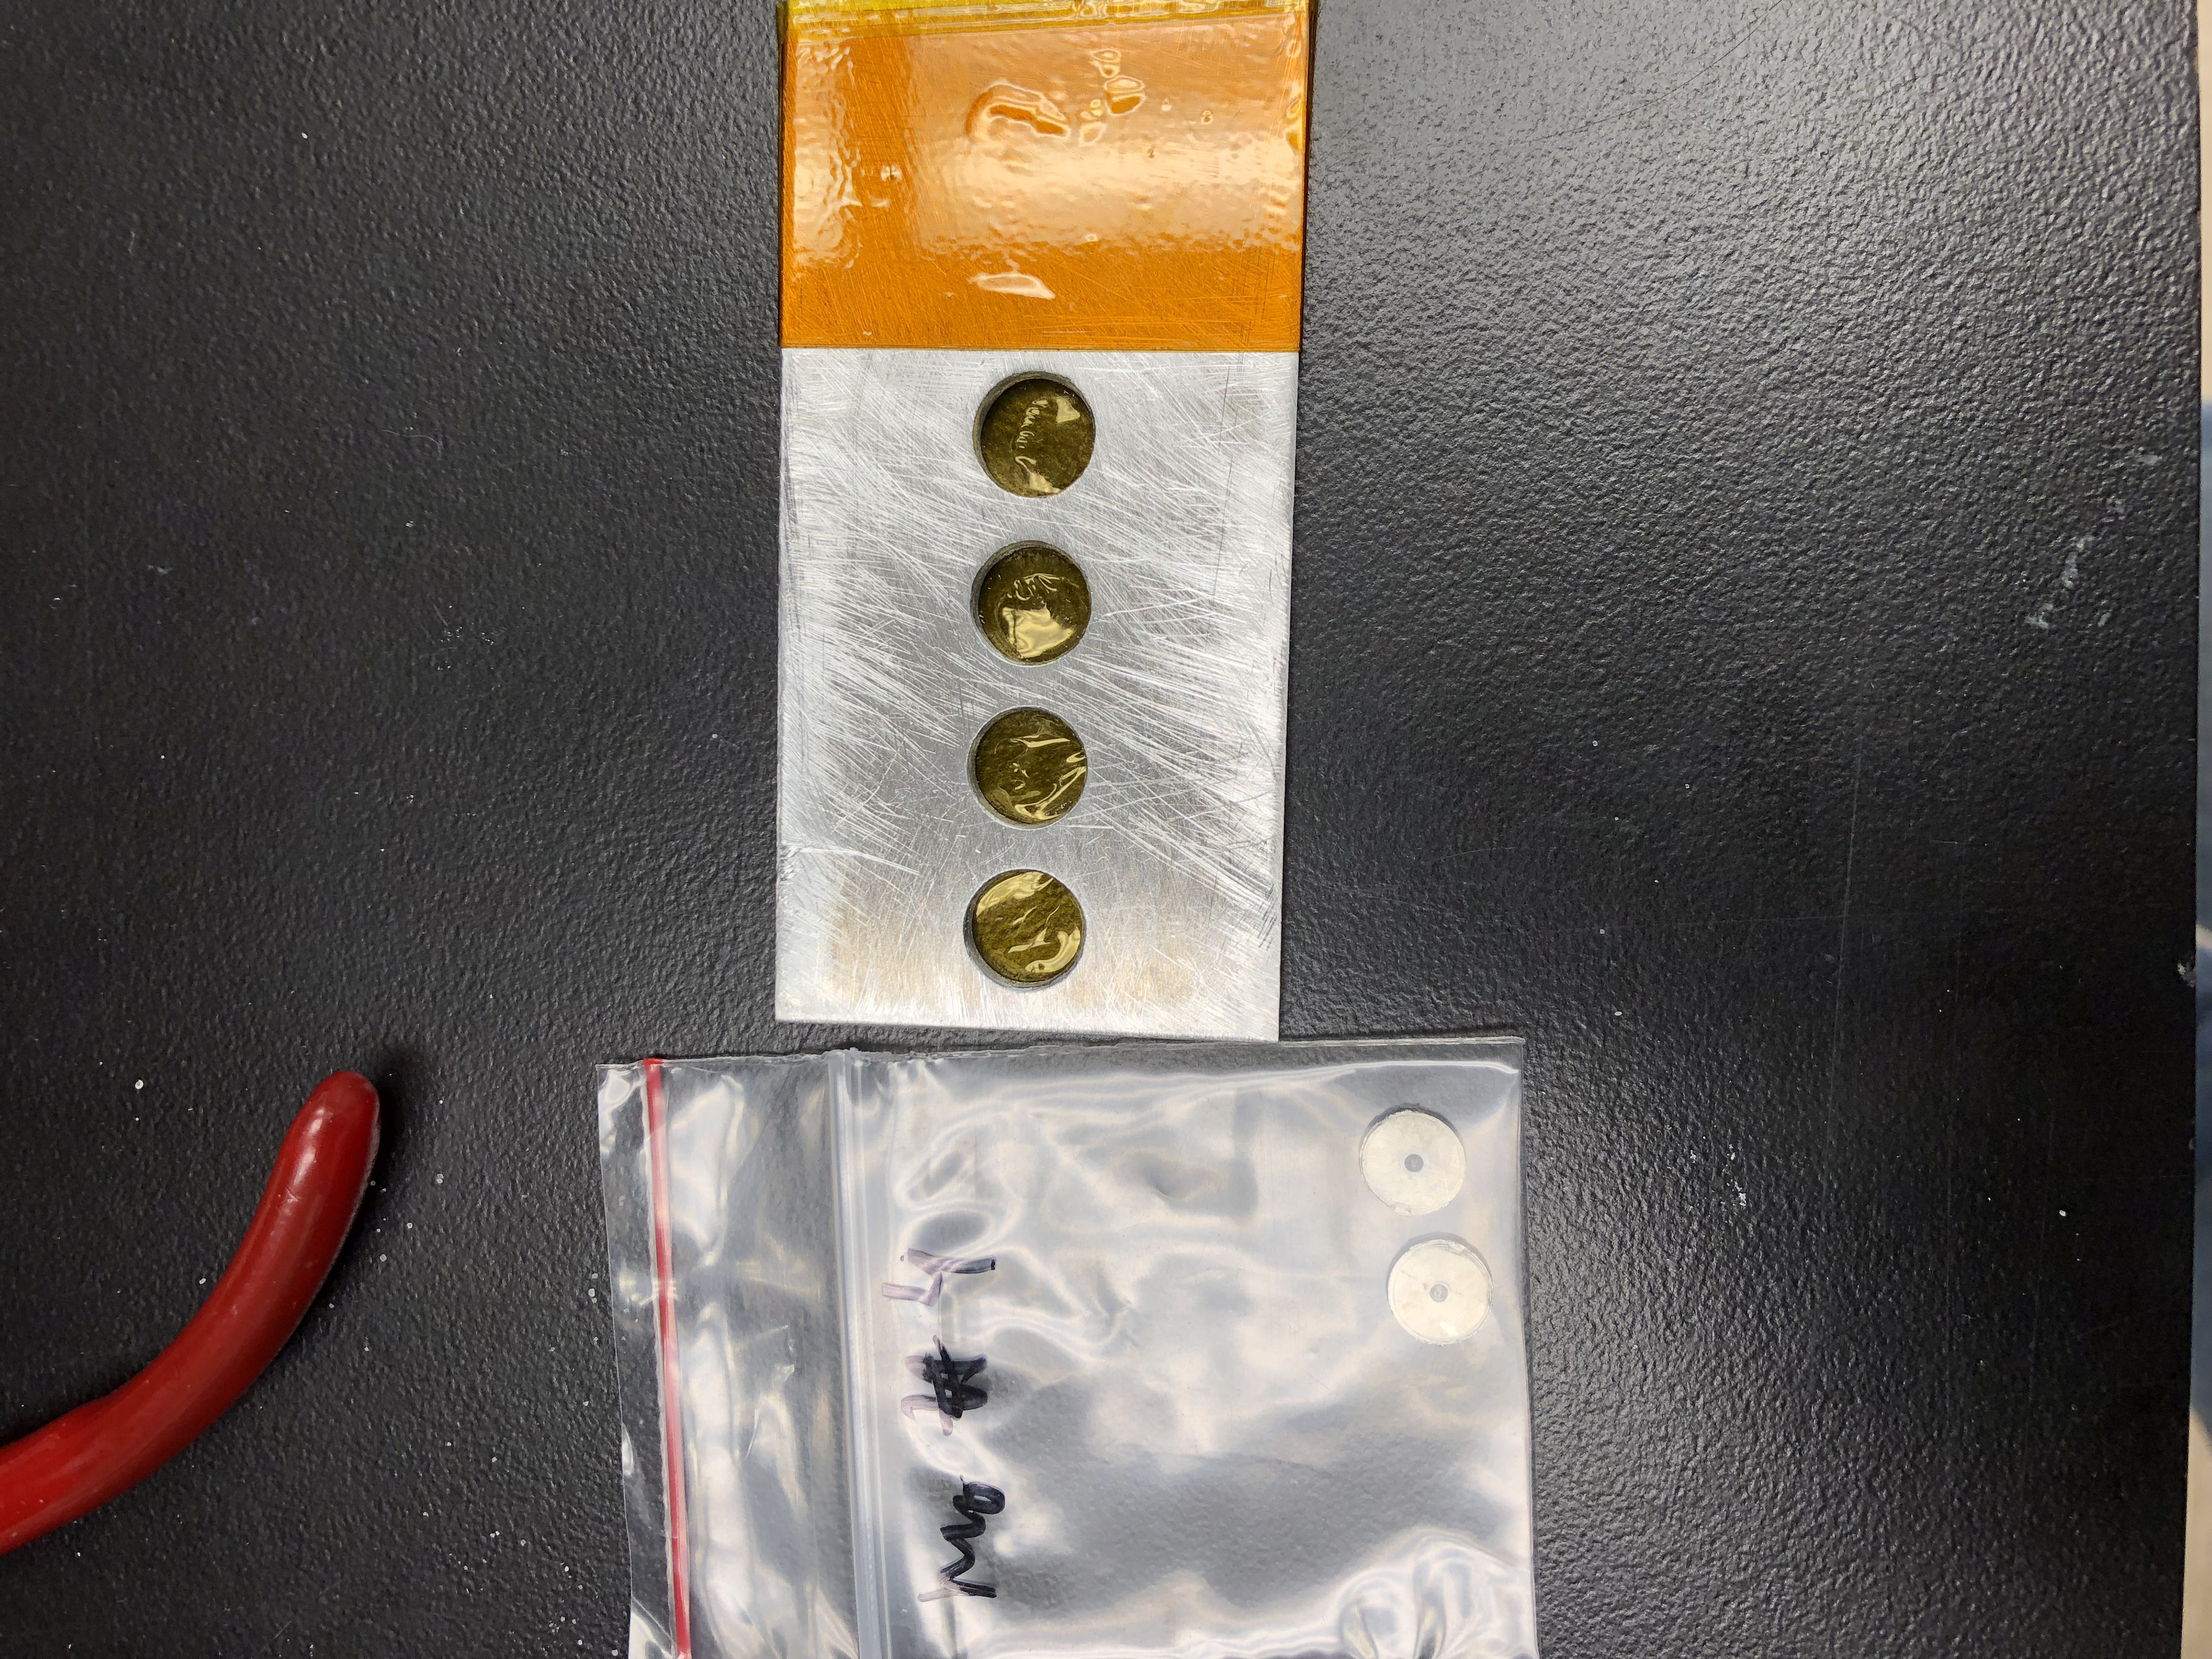
\includegraphics[clip=true,trim=5pt 1000pt 10pt 900pt,width=0.75\columnwidth,angle=90]{./figures/IMG_8840.JPG}
%  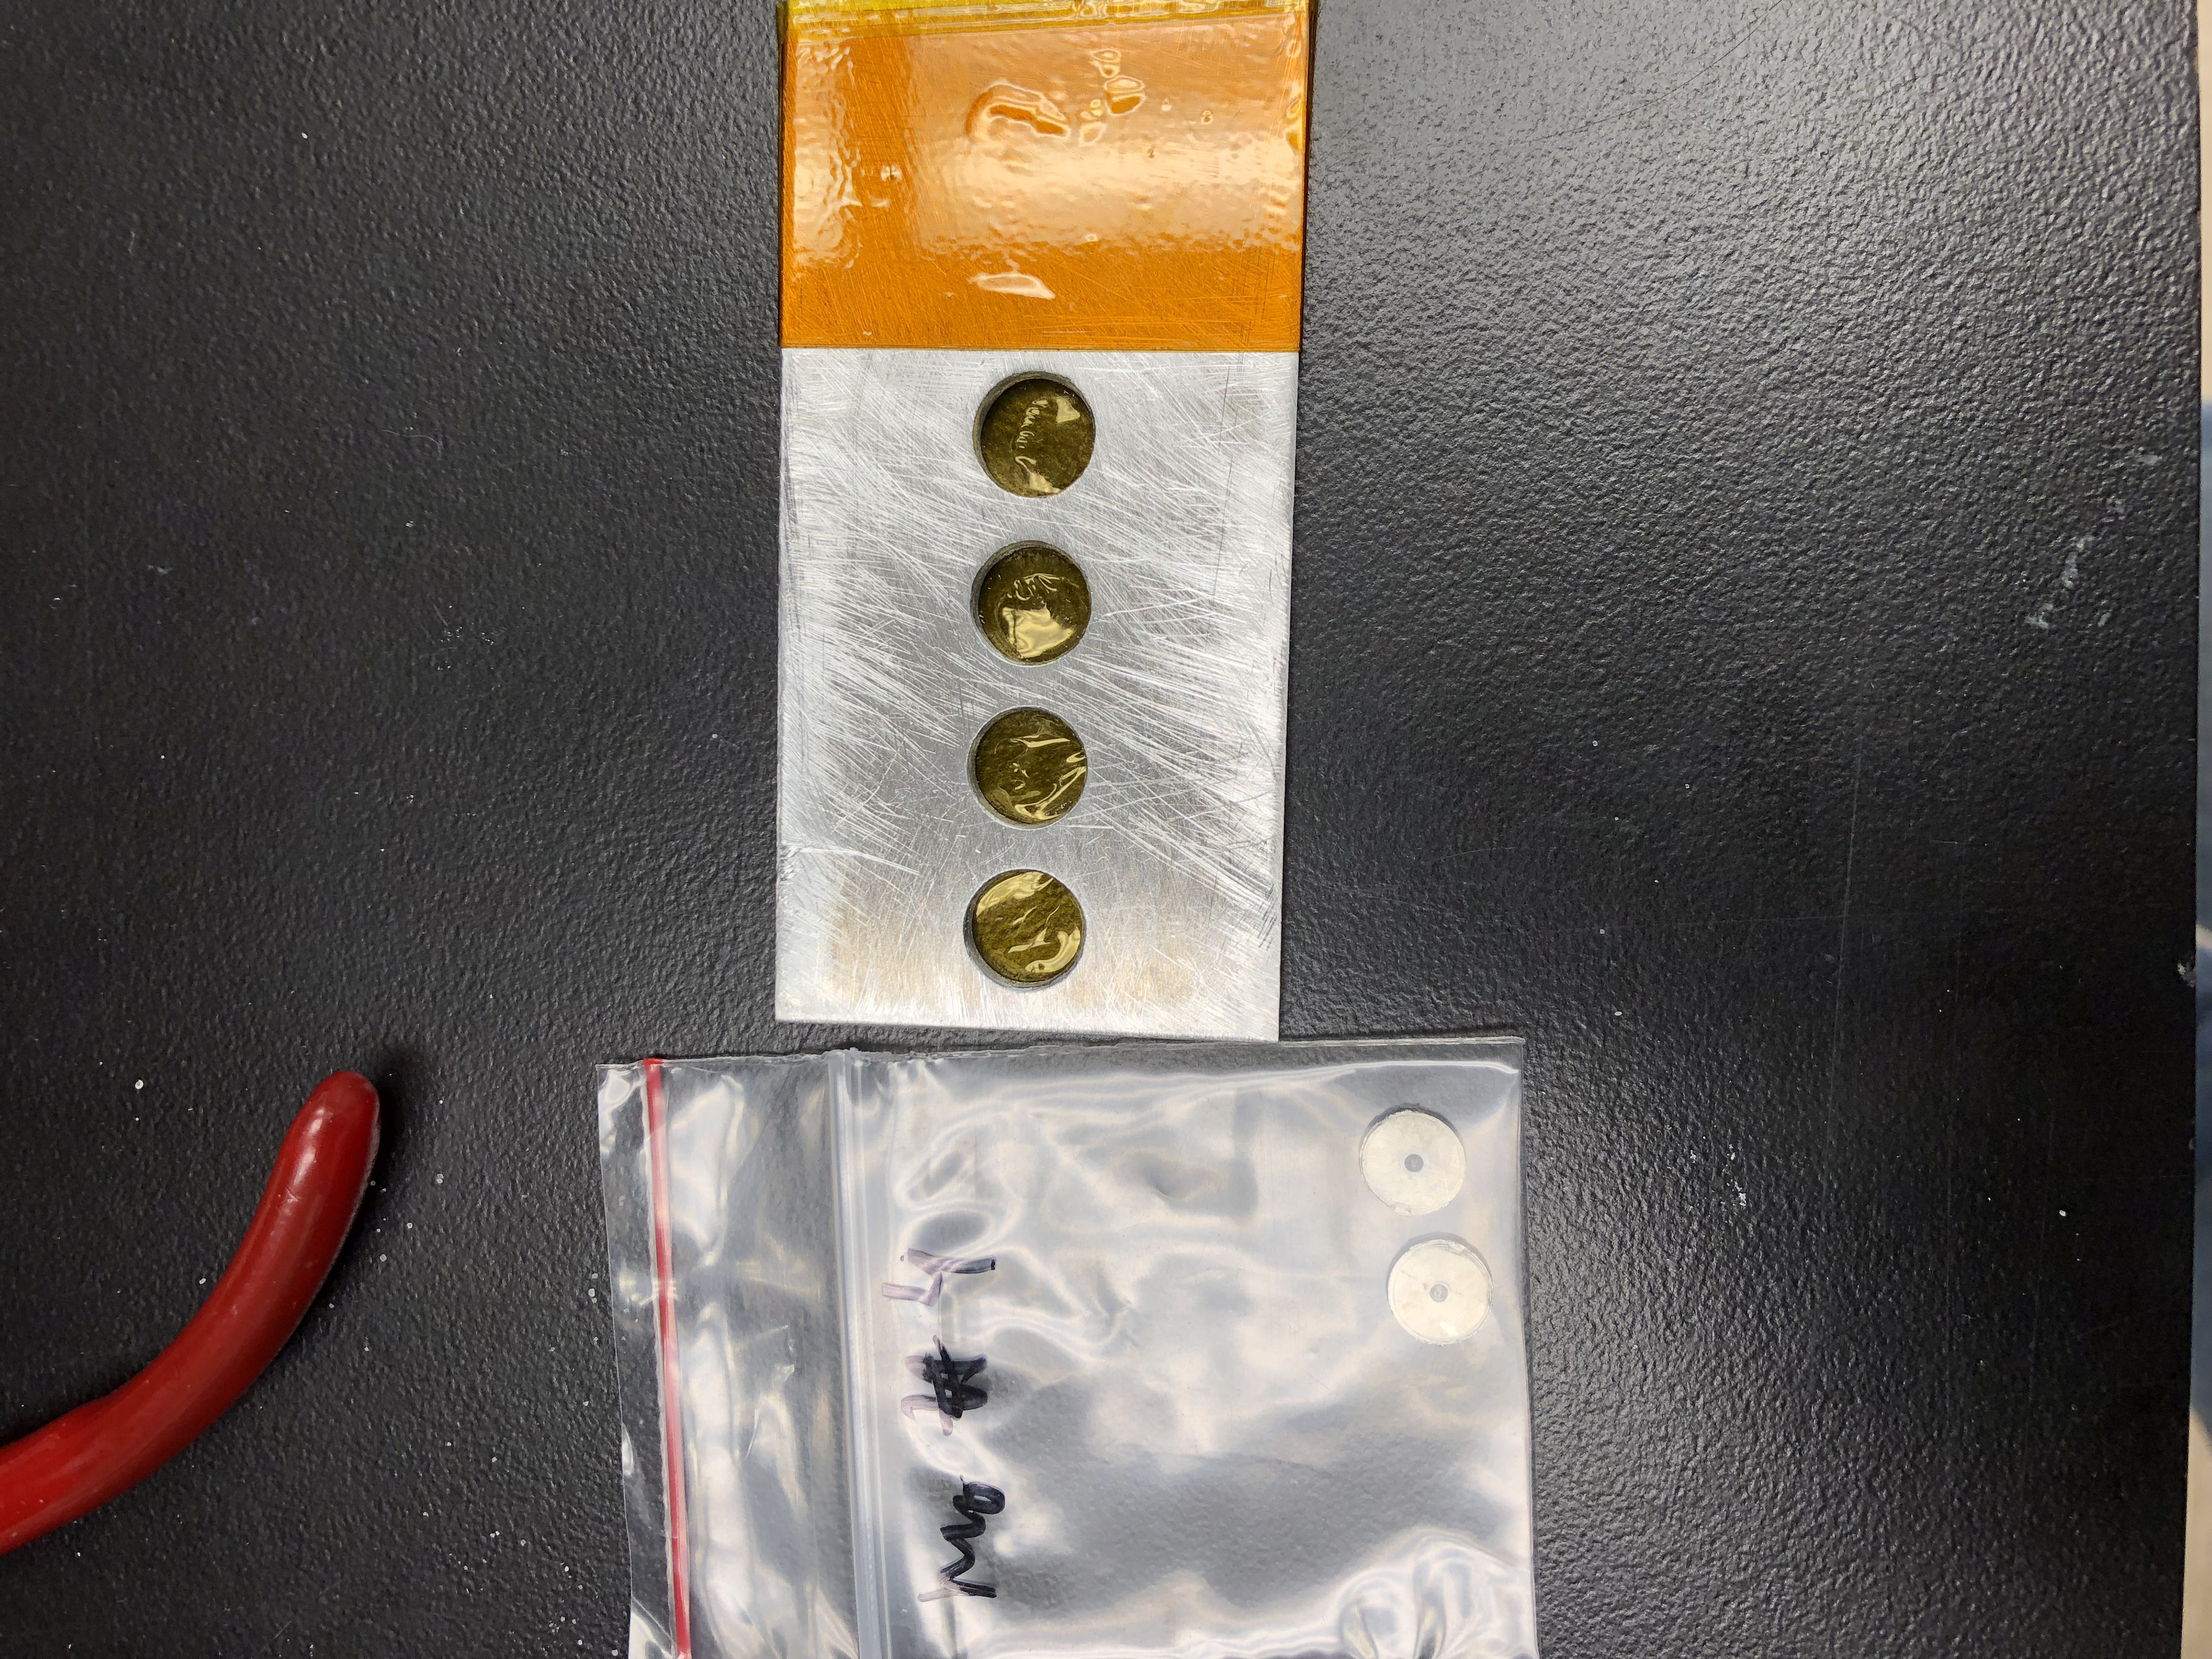
\includegraphics[width=0.75\columnwidth,angle=270]{./figures/IMG_8840.JPG}
 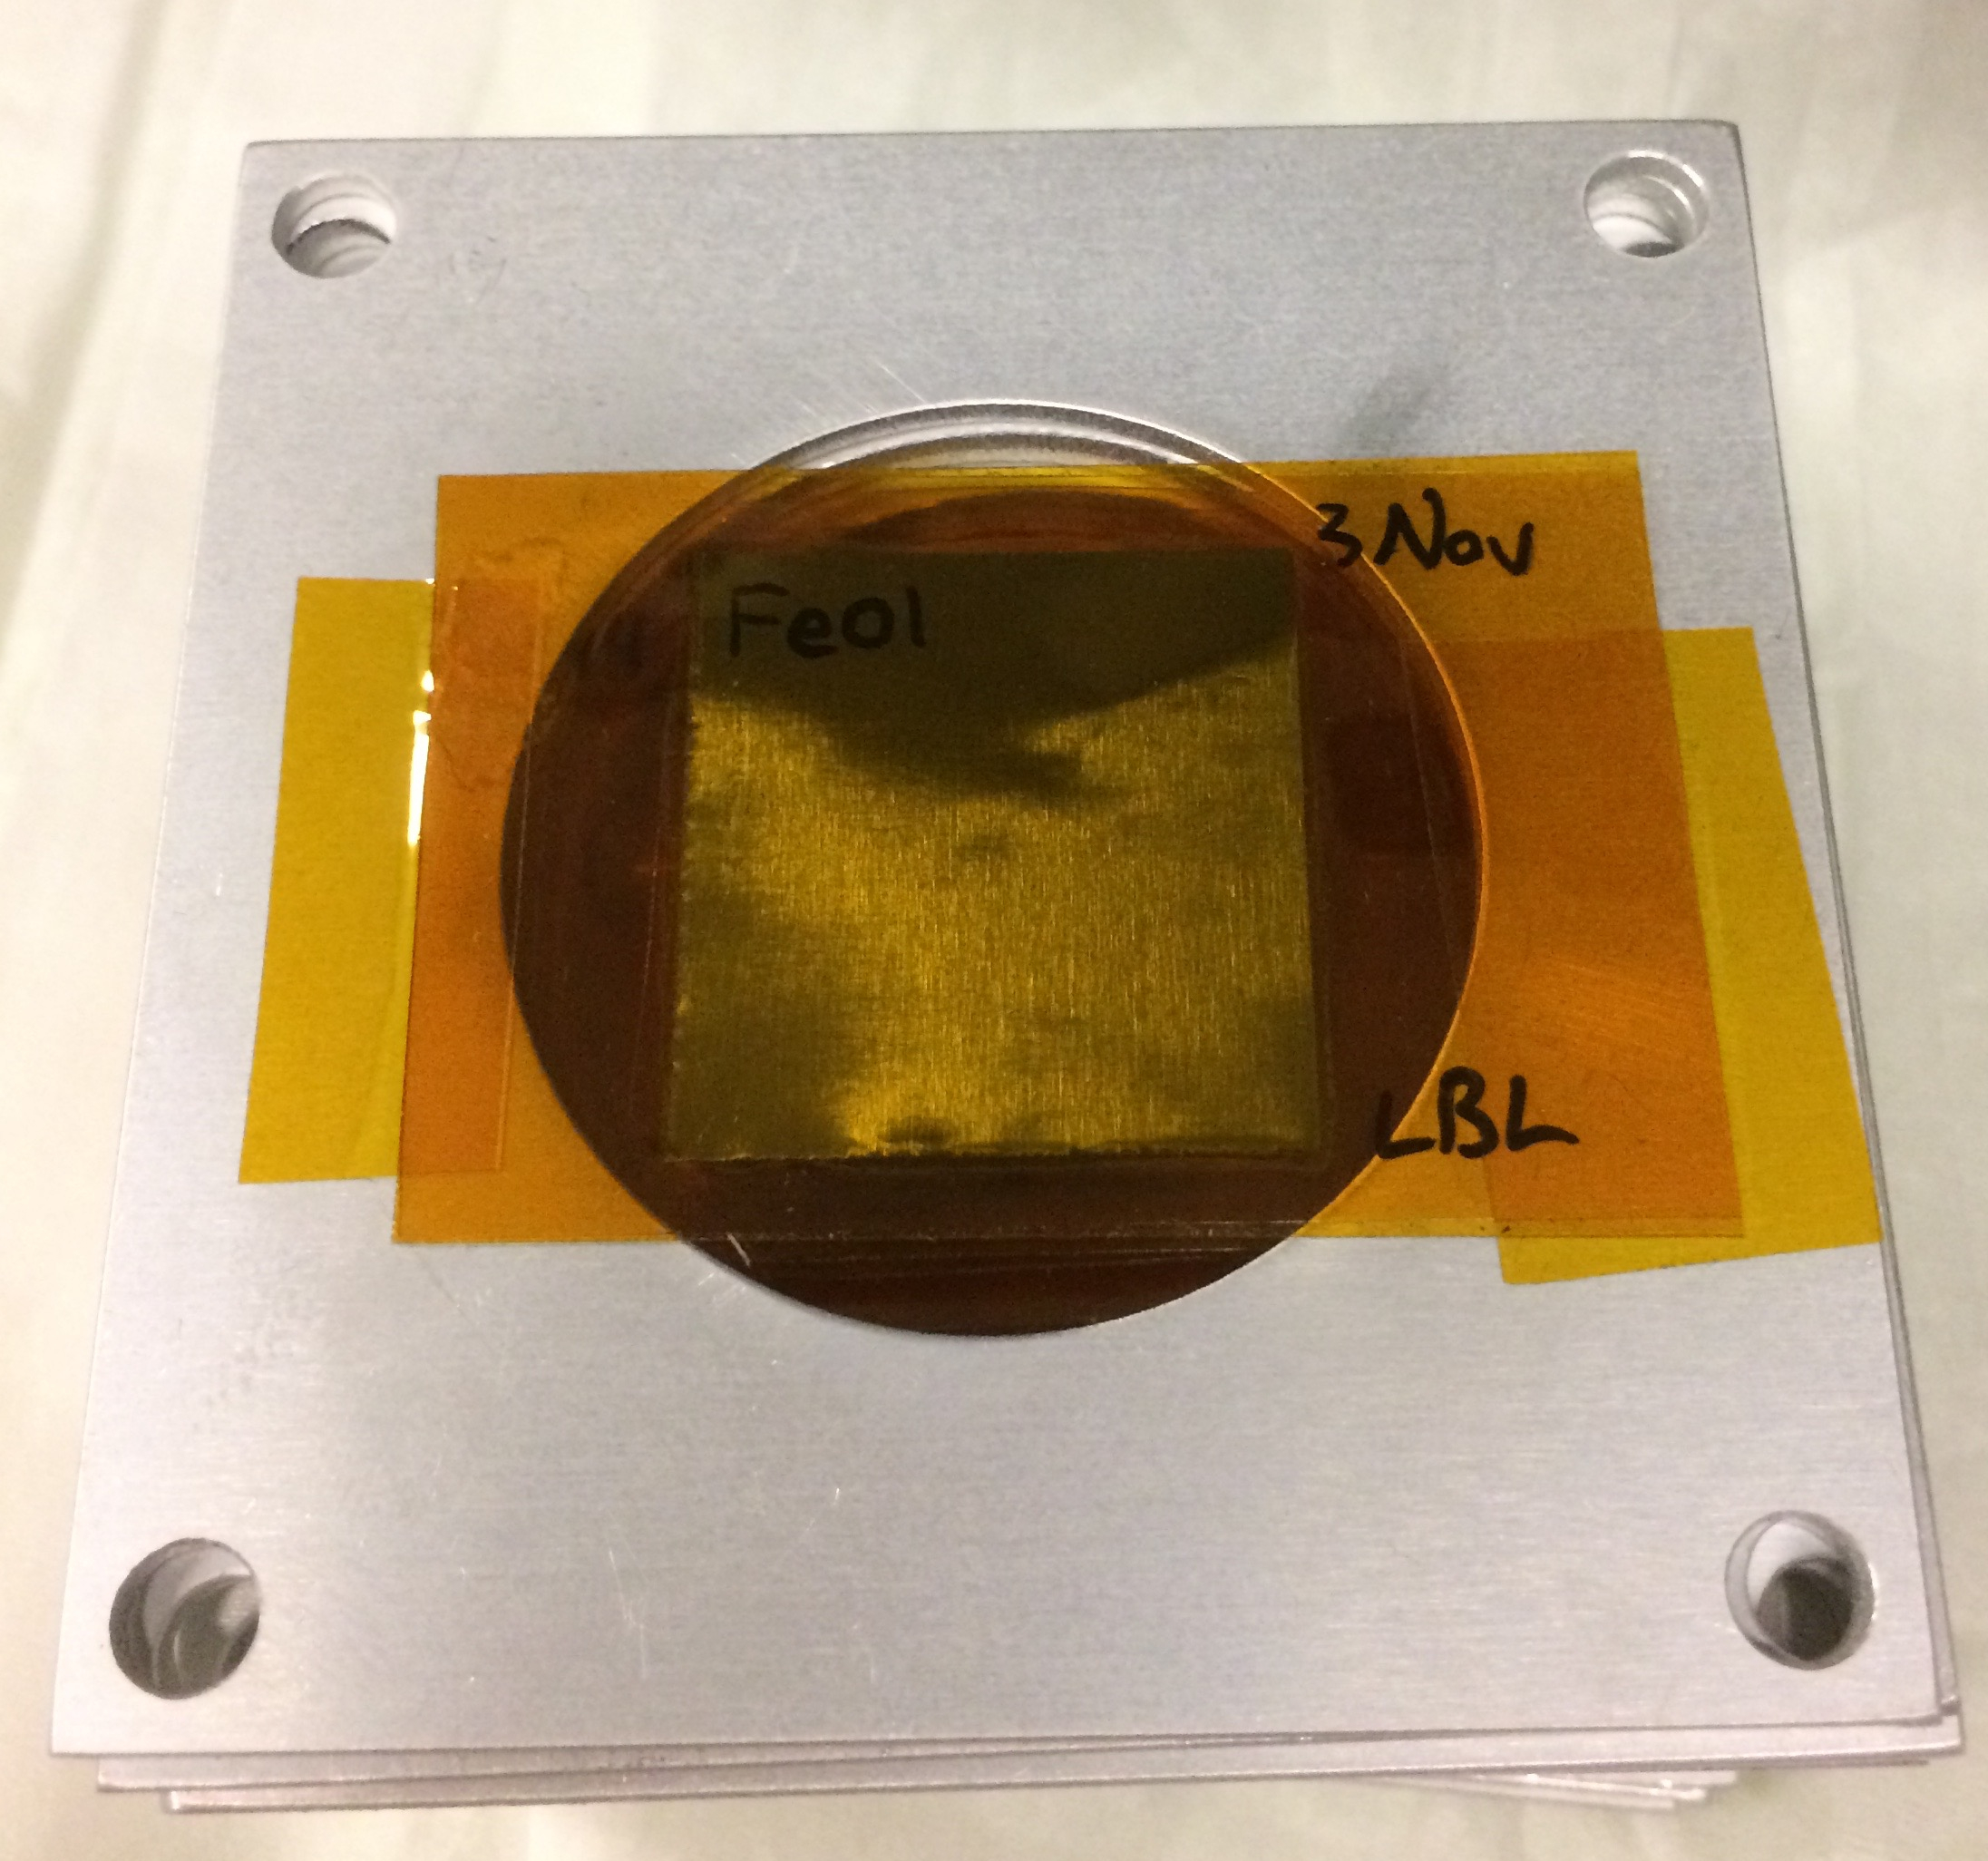
\includegraphics[width=0.5\columnwidth]{./figures/IMG_0305.jpg}
 % IMG_8840.JPG: 4032x3024 pixel, 72dpi, 142.24x106.68 cm, bb=0 0 4032 3024
 \caption{A stack of Fe, Cu, and Ti foils mounted on aluminum frames (Fe-01 visible on top), for the 55\,MeV Fe(p,x) target stack. All foils are mounted over the aperture of a 1.5875 mm-thick aluminum frame.}
 \label{fig:fe_IMG_0305}
\end{figure}



\begin{figure}
 \centering
%                                l   b      r    top
%  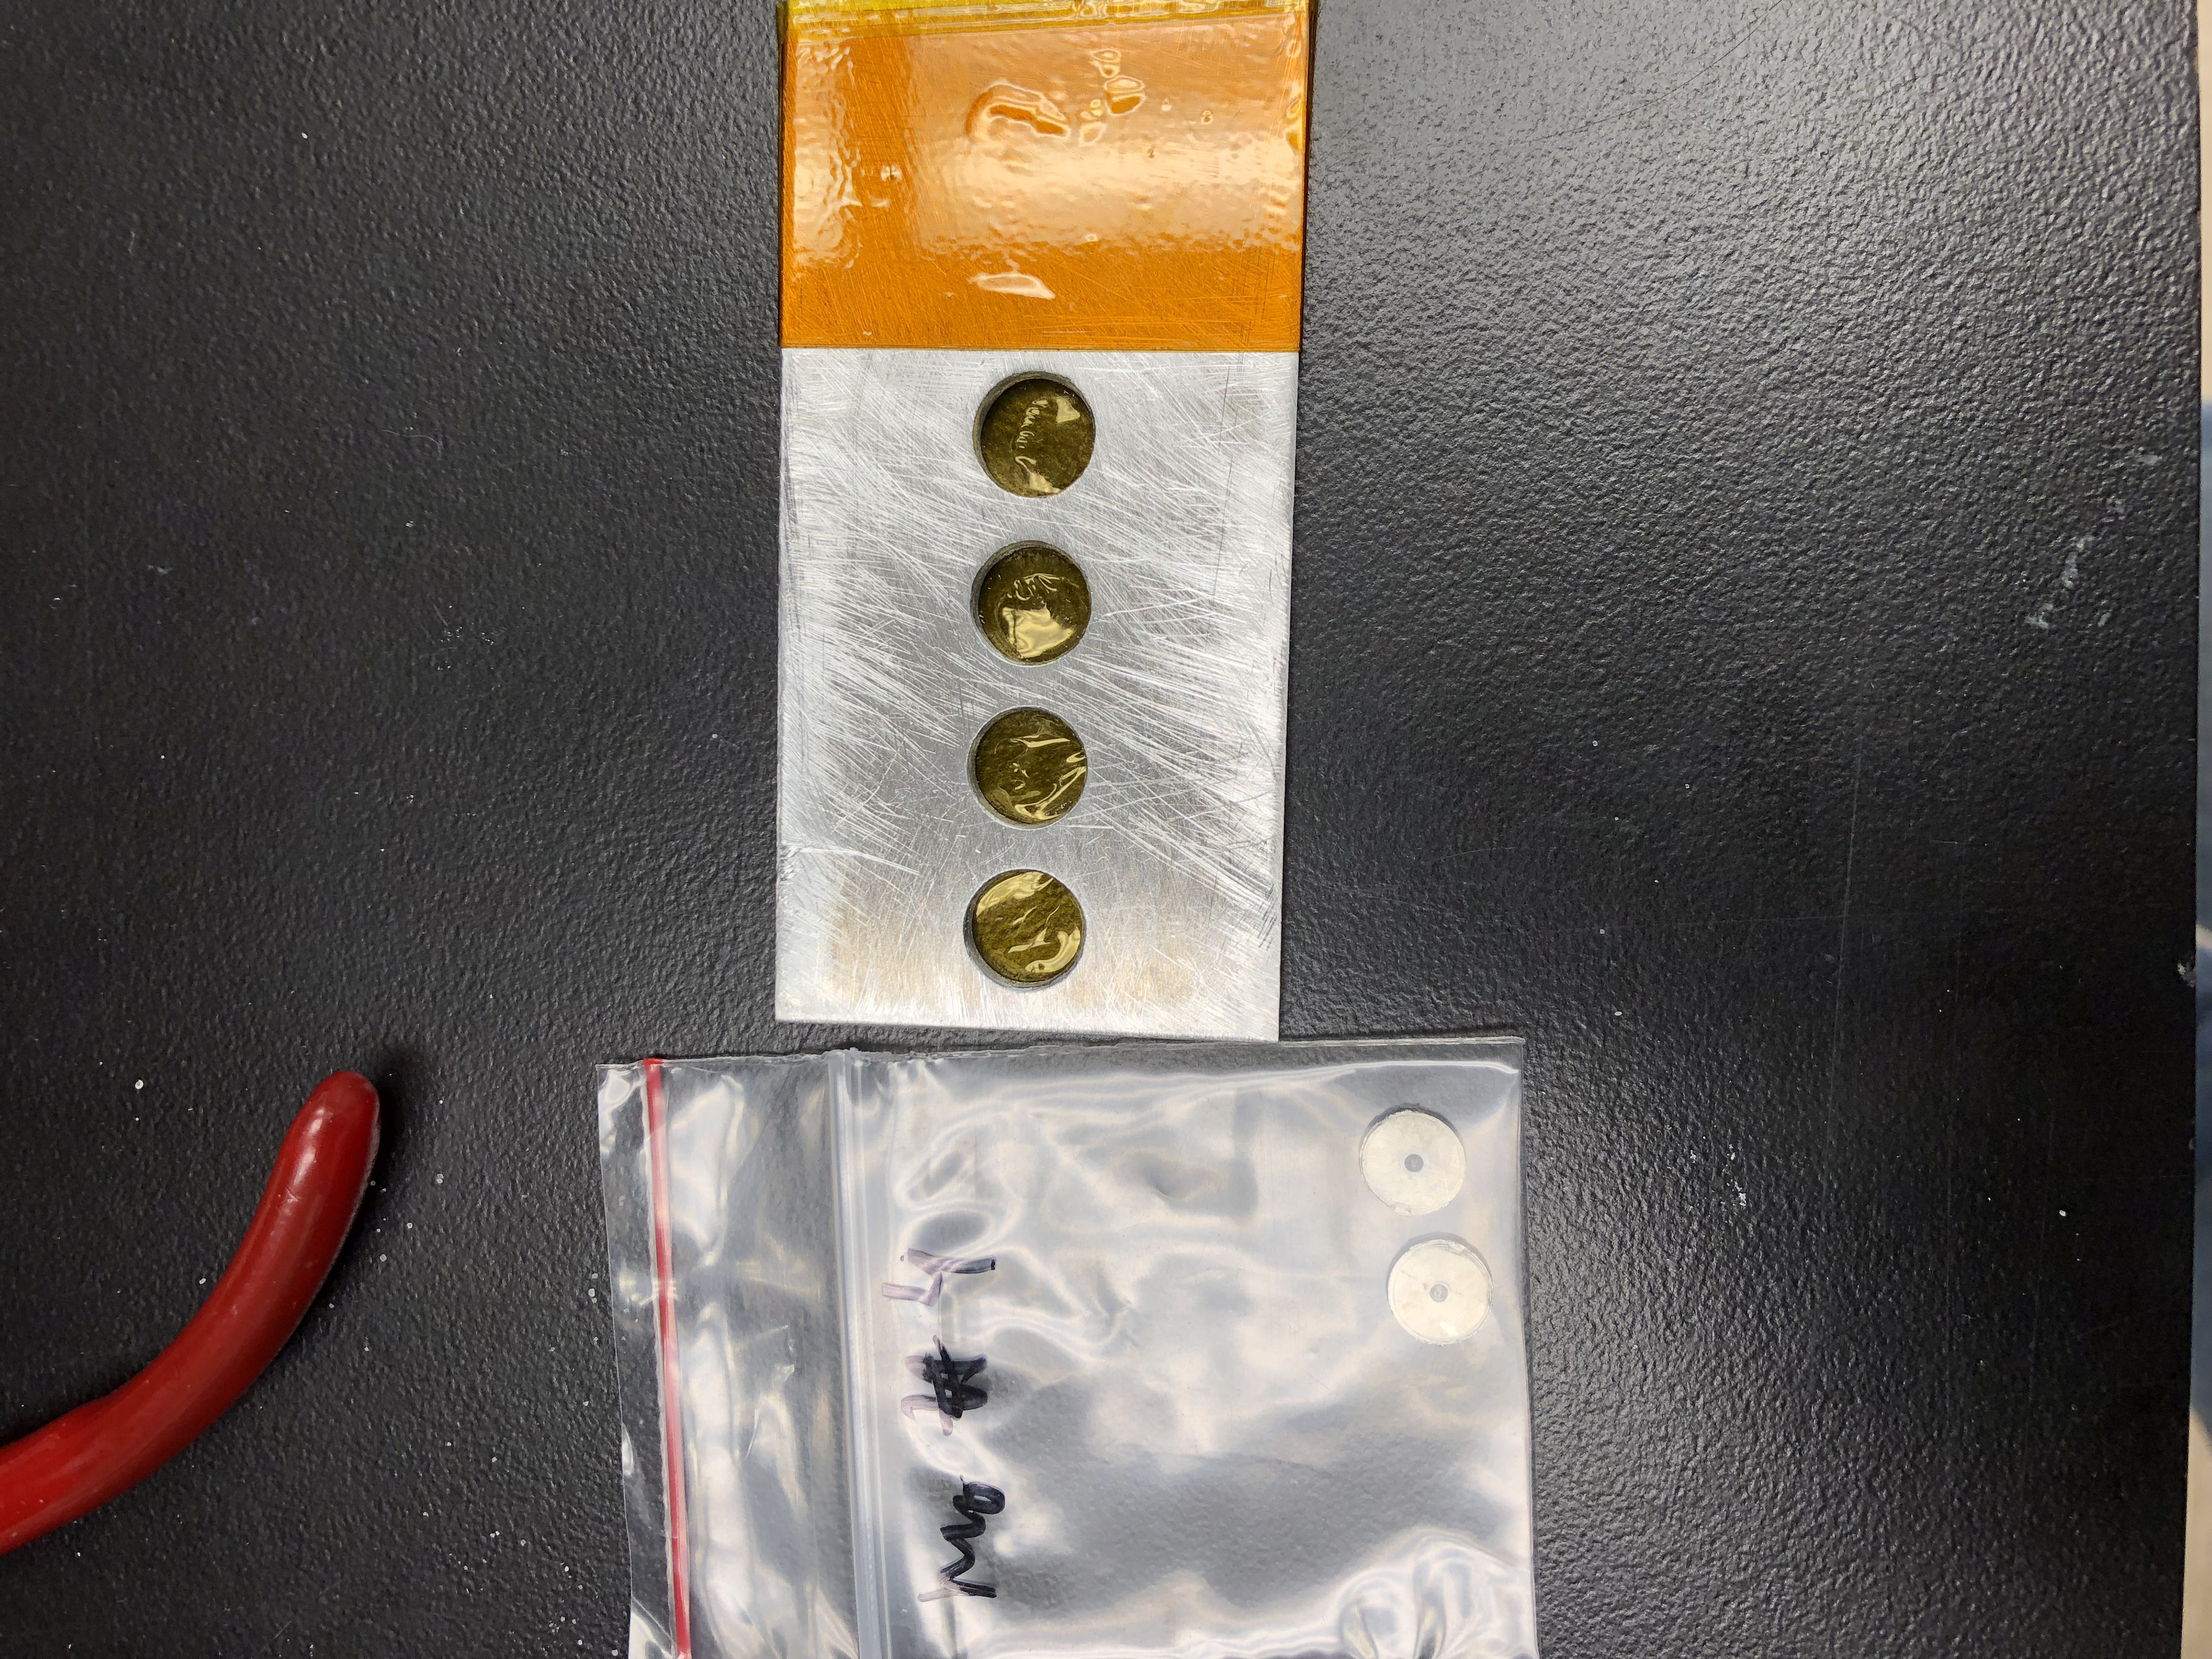
\includegraphics[clip=true,trim=5pt 1000pt 10pt 900pt,width=0.75\columnwidth,angle=90]{./figures/IMG_8840.JPG}
%  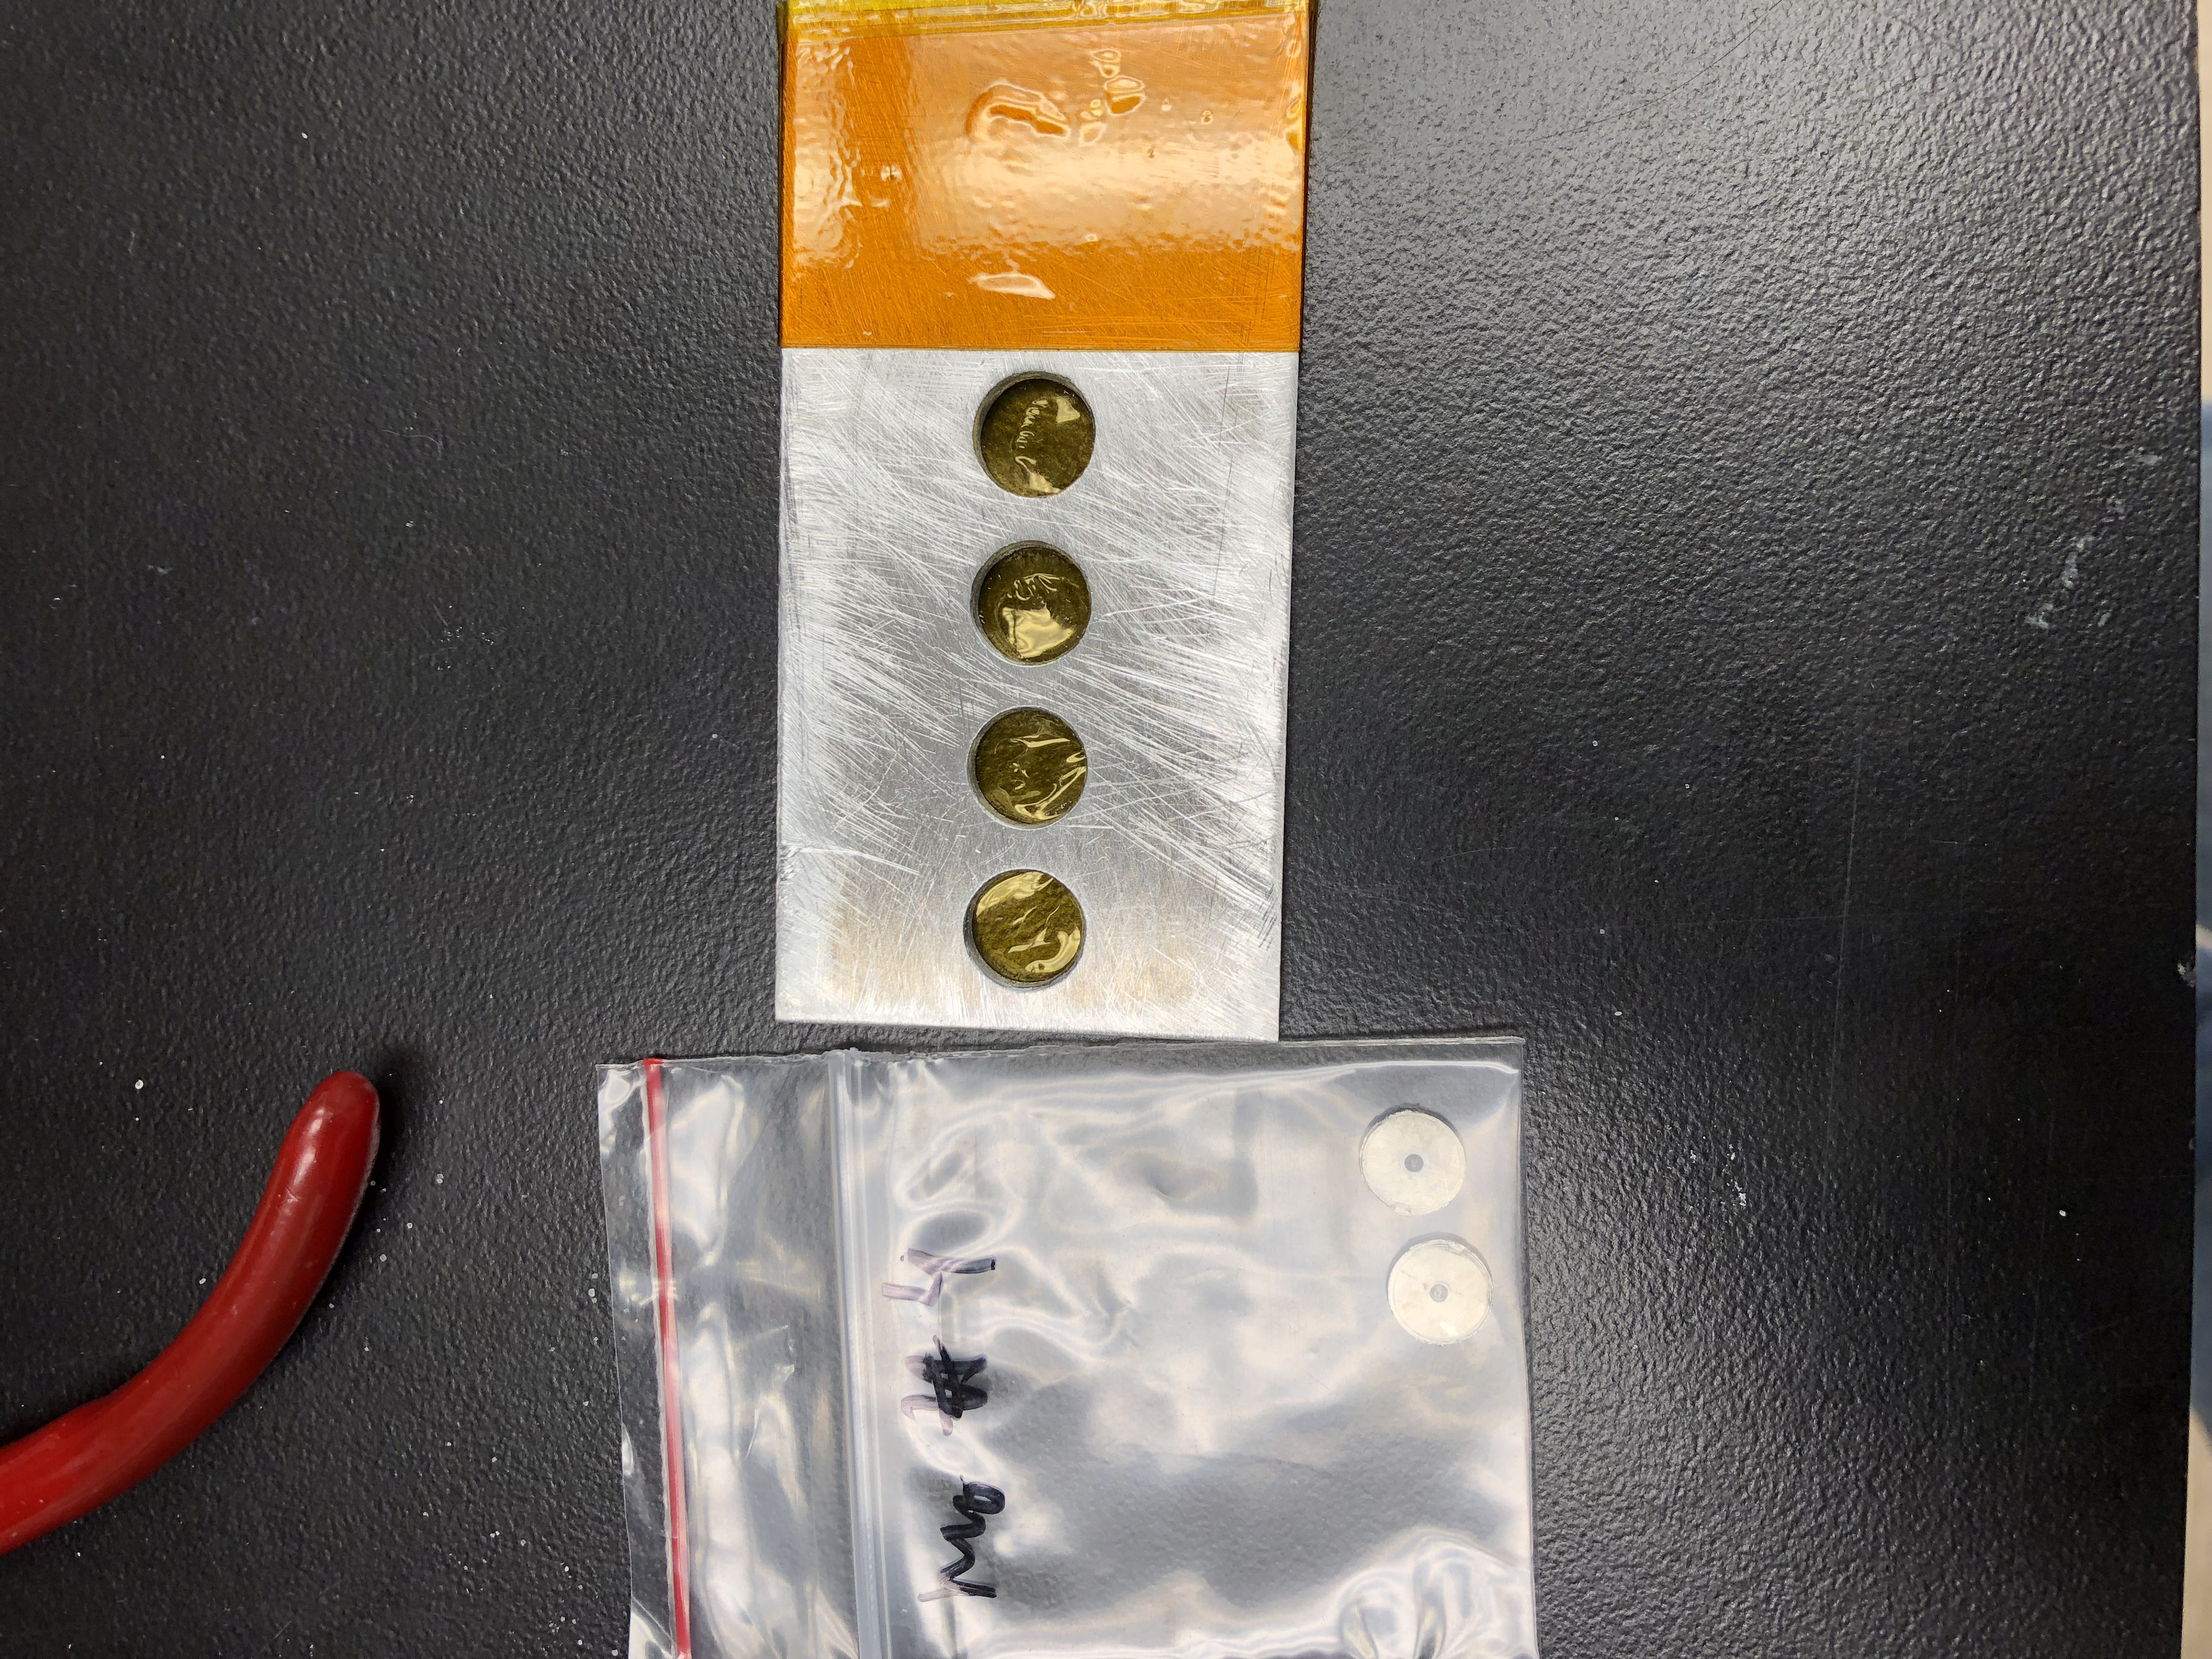
\includegraphics[width=0.75\columnwidth,angle=270]{./figures/IMG_8840.JPG}
 \includegraphics[width=0.75\columnwidth]{./figures/SAM_252_Cu14.JPG}
 % IMG_8840.JPG: 4032x3024 pixel, 72dpi, 142.24x106.68 cm, bb=0 0 4032 3024
 \caption{The ORTEC GMX Series (model \#GMX-50220-S)  High-Purity Germanium detector used for gamma spectroscopy of the activated foils, as described in \autoref{sec:spectroscopy_fe}. The detector, counting foil Cu-14 in this figure, has a \enquote{ladder} permitting counting at various fixed distances (in 1\,cm inetrvals) from the front face of the detector. With the lead shielding lid closed (for reduced background), the ladder permits counting up to 18\,cm, and up to 75\,cm with the lid open.   }
 \label{fig:fe_IMG_1984}
\end{figure}



\subsubsection{MCNP modeling}




A rendering of the 55\,MeV Fe(p,x) target stack, as modeled in MCNP6, is seen in \autoref{fig:fe_vised_55}.
% This figure presents a small subset of the full MCNP6 model of the HFNG,  to better illustrate the geometry of the target chamber.
This model is the same described in \autoref{sec:proton_transport_fe} for simulation of proton transport.
The full input file for this MCNP model is included here for reference, in Appendix \ref{sec:88_mcnp_deck}.
In this figure, the 55\,MeV proton beam enters from the left of the figure, where it is incident (in the positive $x$ direction) upon the \textred{Inconel beam entrance window (yellow).}
The other stack elements, described in  \autoref{tab:fe_stack_table} are illustrated here, as well.
\textred{The green cell is the cooling water channel for the target box, the air filling the target box is shown in light blue, and the 6061 aluminum beam degraders are shown in dark blue.  
The thin black lines seen in between degraders are the Nb, Cu, and Al activation points at each energy position, sealed in Kapton tape. }
The detail of each foil sealed in the Kapton is not visible here, simply due to the size scale of the stack assembly.
Similarly, a rendering of the 25\,MeV Fe(p,x) target stack, as modeled in MCNP6, is seen in \autoref{fig:fe_vised_25}.
% This figure presents a small subset of the full MCNP6 model of the HFNG,  to better illustrate the geometry of the target chamber.
% This model is the same described in \autoref{sec:proton_transport_fe} for simulation of proton transport.
The full input file for this MCNP model is included here for reference, in Appendix \ref{sec:88_mcnp_deck_lowE}.






\begin{figure}
 \centering
 %trim option's parameter order: left bottom right top
 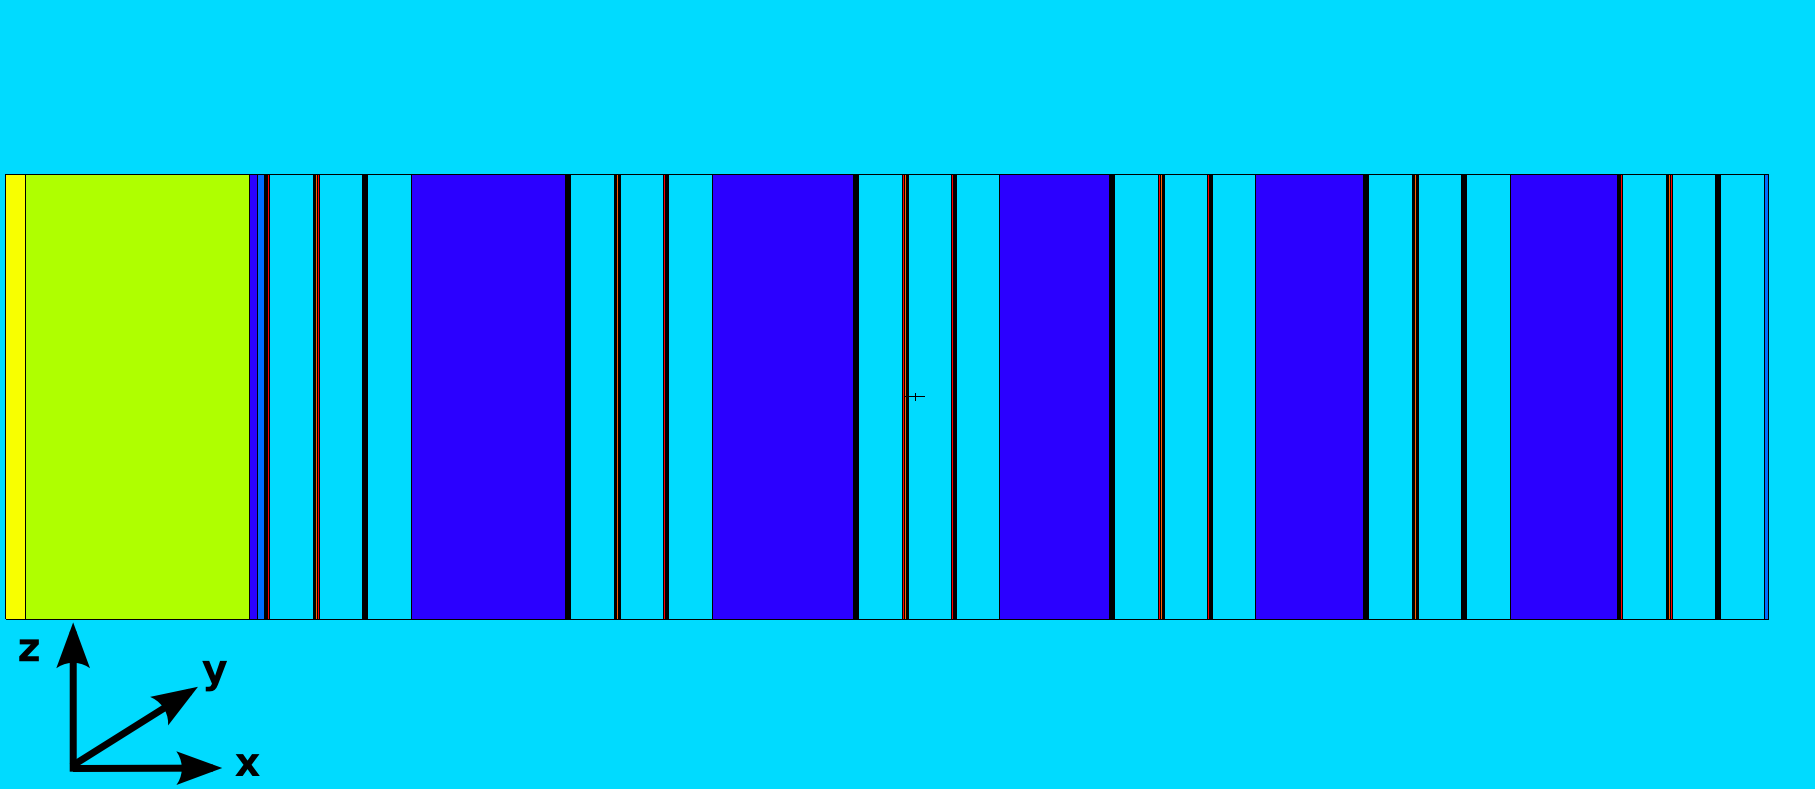
\includegraphics[trim = 0mm 0mm 2mm 0mm, clip,width=0.75\columnwidth]{./figures/ipf_stack_nolabels_axes.PNG}
 % mcnp_vised2.PNG.png: 688x443 pixel, 96dpi, 18.21x11.72 cm, bb=0 0 516 332
%   \caption{Simplified top-down MCNP6 model of the IPF Nb(p,x) target stack. The 100\,MeV proton beam enters from the left of the figure, where it is incident upon the Inconel beam entrance window (yellow). The beam is transported down the length of the stack, towards the rear of the stack on the right side of the figure.
 \caption{\textred{Update this figure!!!} Simplified top-down MCNP6 model of the 55\,MeV Fe(p,x) target stack. The  proton beam enters from the left of the figure, where it is incident upon the \textred{Inconel beam entrance window (yellow).} The beam is transported down the length of the stack, towards the rear of the stack on the right side of the figure.
%  MCNP6 model of the HFNG target chamber, with reference scale. The co-loaded foils can be seen in the target chamber center.  The ovals indicate the location of water cooling channels.
}
 \label{fig:fe_vised_55}
\end{figure}


\begin{figure}
 \centering
 %trim option's parameter order: left bottom right top
 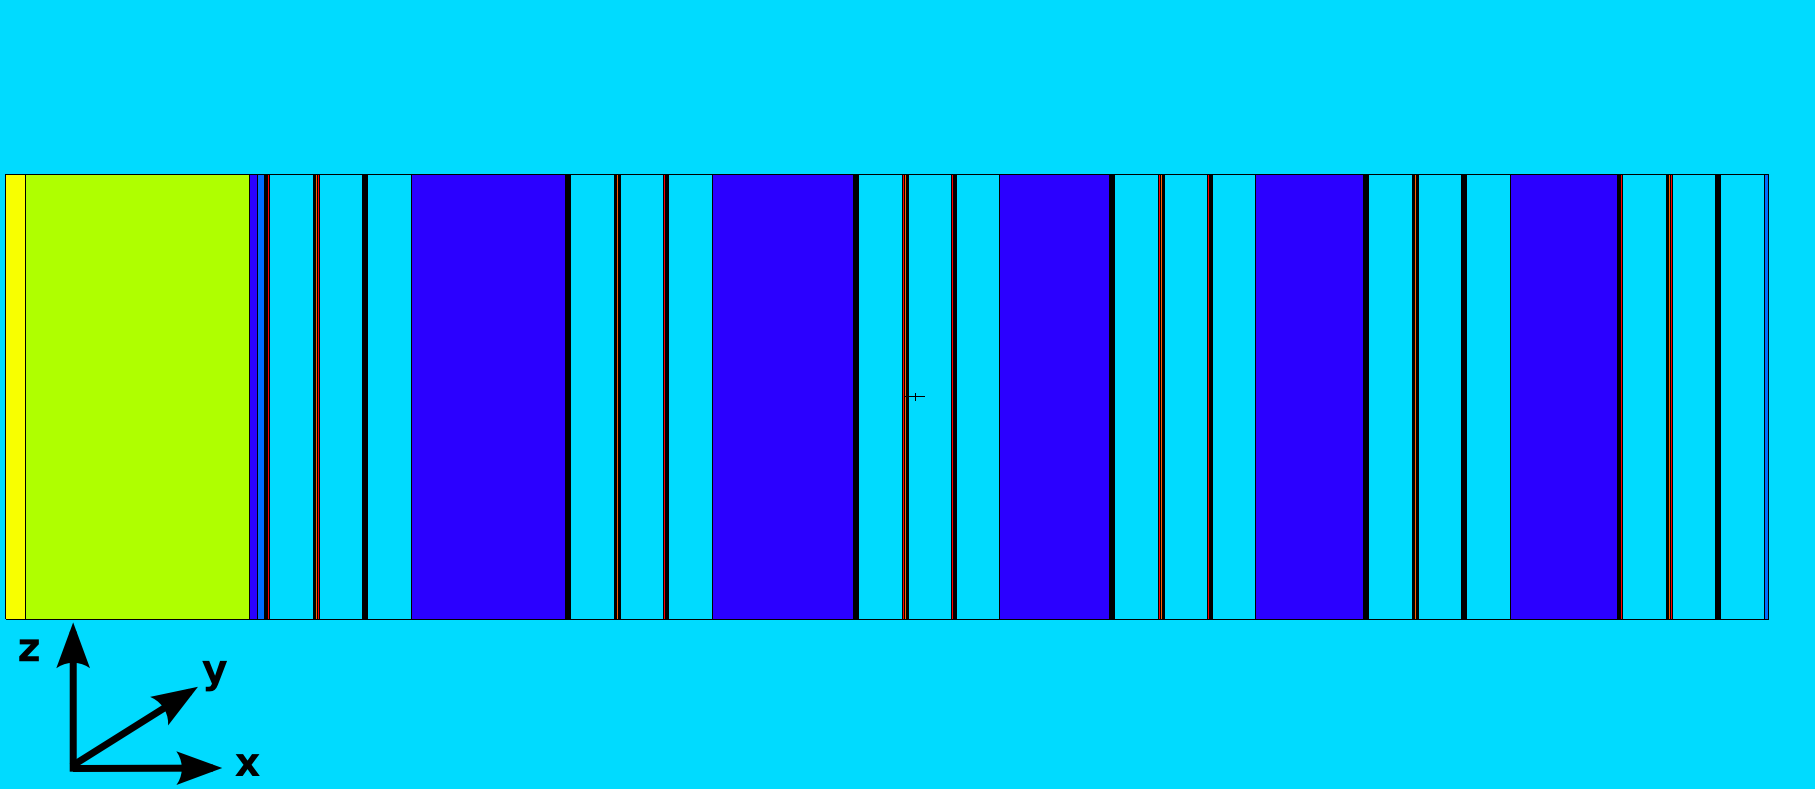
\includegraphics[trim = 0mm 0mm 2mm 0mm, clip,width=0.75\columnwidth]{./figures/ipf_stack_nolabels_axes.PNG}
 % mcnp_vised2.PNG.png: 688x443 pixel, 96dpi, 18.21x11.72 cm, bb=0 0 516 332
%   \caption{Simplified top-down MCNP6 model of the IPF Nb(p,x) target stack. The 100\,MeV proton beam enters from the left of the figure, where it is incident upon the Inconel beam entrance window (yellow). The beam is transported down the length of the stack, towards the rear of the stack on the right side of the figure.
\caption{\textred{Update this figure!!!} Simplified top-down MCNP6 model of the 25\,MeV  Fe(p,x) target stack. The  proton beam enters from the left of the figure, where it is incident upon \textred{the Inconel beam entrance window (yellow)}. The beam is transported down the length of the stack, towards the rear of the stack on the right side of the figure.
%  MCNP6 model of the HFNG target chamber, with reference scale. The co-loaded foils can be seen in the target chamber center.  The ovals indicate the location of water cooling channels.
}
 \label{fig:fe_vised_25}
\end{figure}





\begin{figure*}
    \centering    
    \subfloat{
        \centering
%         \includegraphics[width=\textwidth]{./figures/target2.png}
        \subfigimg[width=0.495\textwidth]{a)}{./figures/Al_ptallies.pdf}{80}
%         \caption{Decay curve for the $\beta^-$ decay of \ce{^{116}In}.}
        %         \refstepcounter{subfigure}
%          \label{fig:91mNb}
%    }
%      \subfloat{
%         \centering
%         \includegraphics[width=\columnwidth]{./figures/Capture.PNG}
        \subfigimg[width=0.495\textwidth]{b)}{./figures/Cu_ptallies.pdf}{80}
%         \caption{ Decay curve for the $\beta^+$ decay of \ce{^{64}Cu}.}
%         \refstepcounter{subfigure} 
%         \label{fig:92mNb}
   \hspace{-10pt}}%
    \caption{\textred{Update this figure!!!} Final variance minimized incident proton energy distributions for the (a) Cu and (b) Ti foils, as simulated in MCNP6. The distribution tallies in each foil are all normalized to be per source proton, which was $10^8$ in all simulations. As the beam is degraded, proton energy distributions become visibly broadened due to straggling, and drop in magnitude due to scattering losses.}
%      \phantomcaption{}
     \label{fig:fe_ptallies_appendix}
\end{figure*}



Using this MCNP6 model, the proton energy distribution is tallied in all volumes of the stack assembly.
As seen in \autoref{fig:Fe_ptallies} of \autoref{sec:proton_transport_fe}, the corresponding incident proton  energy distributions $\frac{d\phi}{dE}$ from MCNP6 simulation (using the variance minimized degrader density) are shown for the six irradiated Cu and Ti  foils in \autoref{fig:fe_ptallies_appendix}. 
In addition, the MCNP6 model tracks the production and transport of secondary neutrons produced through (p,xn) reactions on the target stack components.
The the proton energy distribution is tallied in all Ti, Cu, and Fe foils, and is seen in \autoref{fig:fe_ntallies}. 
The neutron flux is consistently 3--4 orders of magnitude smaller than the corresponding proton flux, and is seen to be visibly  downscattered when moving down the stack.

\begin{figure*}
    \centering    
    \subfloat{
        \centering
%         \includegraphics[width=\textwidth]{./figures/target2.png}
        \subfigimg[width=0.497\textwidth]{a)}{./figures/Al_ntallies.pdf}{50}
%         \caption{Decay curve for the $\beta^-$ decay of \ce{^{116}In}.}
        %         \refstepcounter{subfigure}
%          \label{fig:91mNb}
%    }
%      \subfloat{
%         \centering
%         \includegraphics[width=\columnwidth]{./figures/Capture.PNG}
        \subfigimg[width=0.497\textwidth]{b)}{./figures/Cu_ntallies.pdf}{50}
%         \caption{ Decay curve for the $\beta^+$ decay of \ce{^{64}Cu}.}
%         \refstepcounter{subfigure} 
%         \label{fig:92mNb}
   \hspace{-10pt}}%
    \\
    \subfloat{
        \centering
%         \includegraphics[width=\columnwidth]{./figures/Capture.PNG}
        \subfigimg[width=0.497\textwidth]{c)}{./figures/Nb_ntallies.pdf}{50}
%         \caption{ Decay curve for the isomeric transition of \ce{^{115m}In}.}
%         \refstepcounter{subfigure}
%          \label{fig:93mMo}
   }%
    \caption{\textred{Update this figure!!!} Final variance minimized incident neutron energy distributions for the (a) Cu, (b) Ti, and (C) Fe foils, as simulated in MCNP6. The distribution tallies in each foil are all normalized to be per source proton, which was $10^8$ in all simulations. As the beam is degraded, neutron energy distributions become visibly downscattered.}
%      \phantomcaption{}
     \label{fig:fe_ntallies}
\end{figure*}





% \begin{figure}
%  \centering
% %                                l   b      r    top
% %  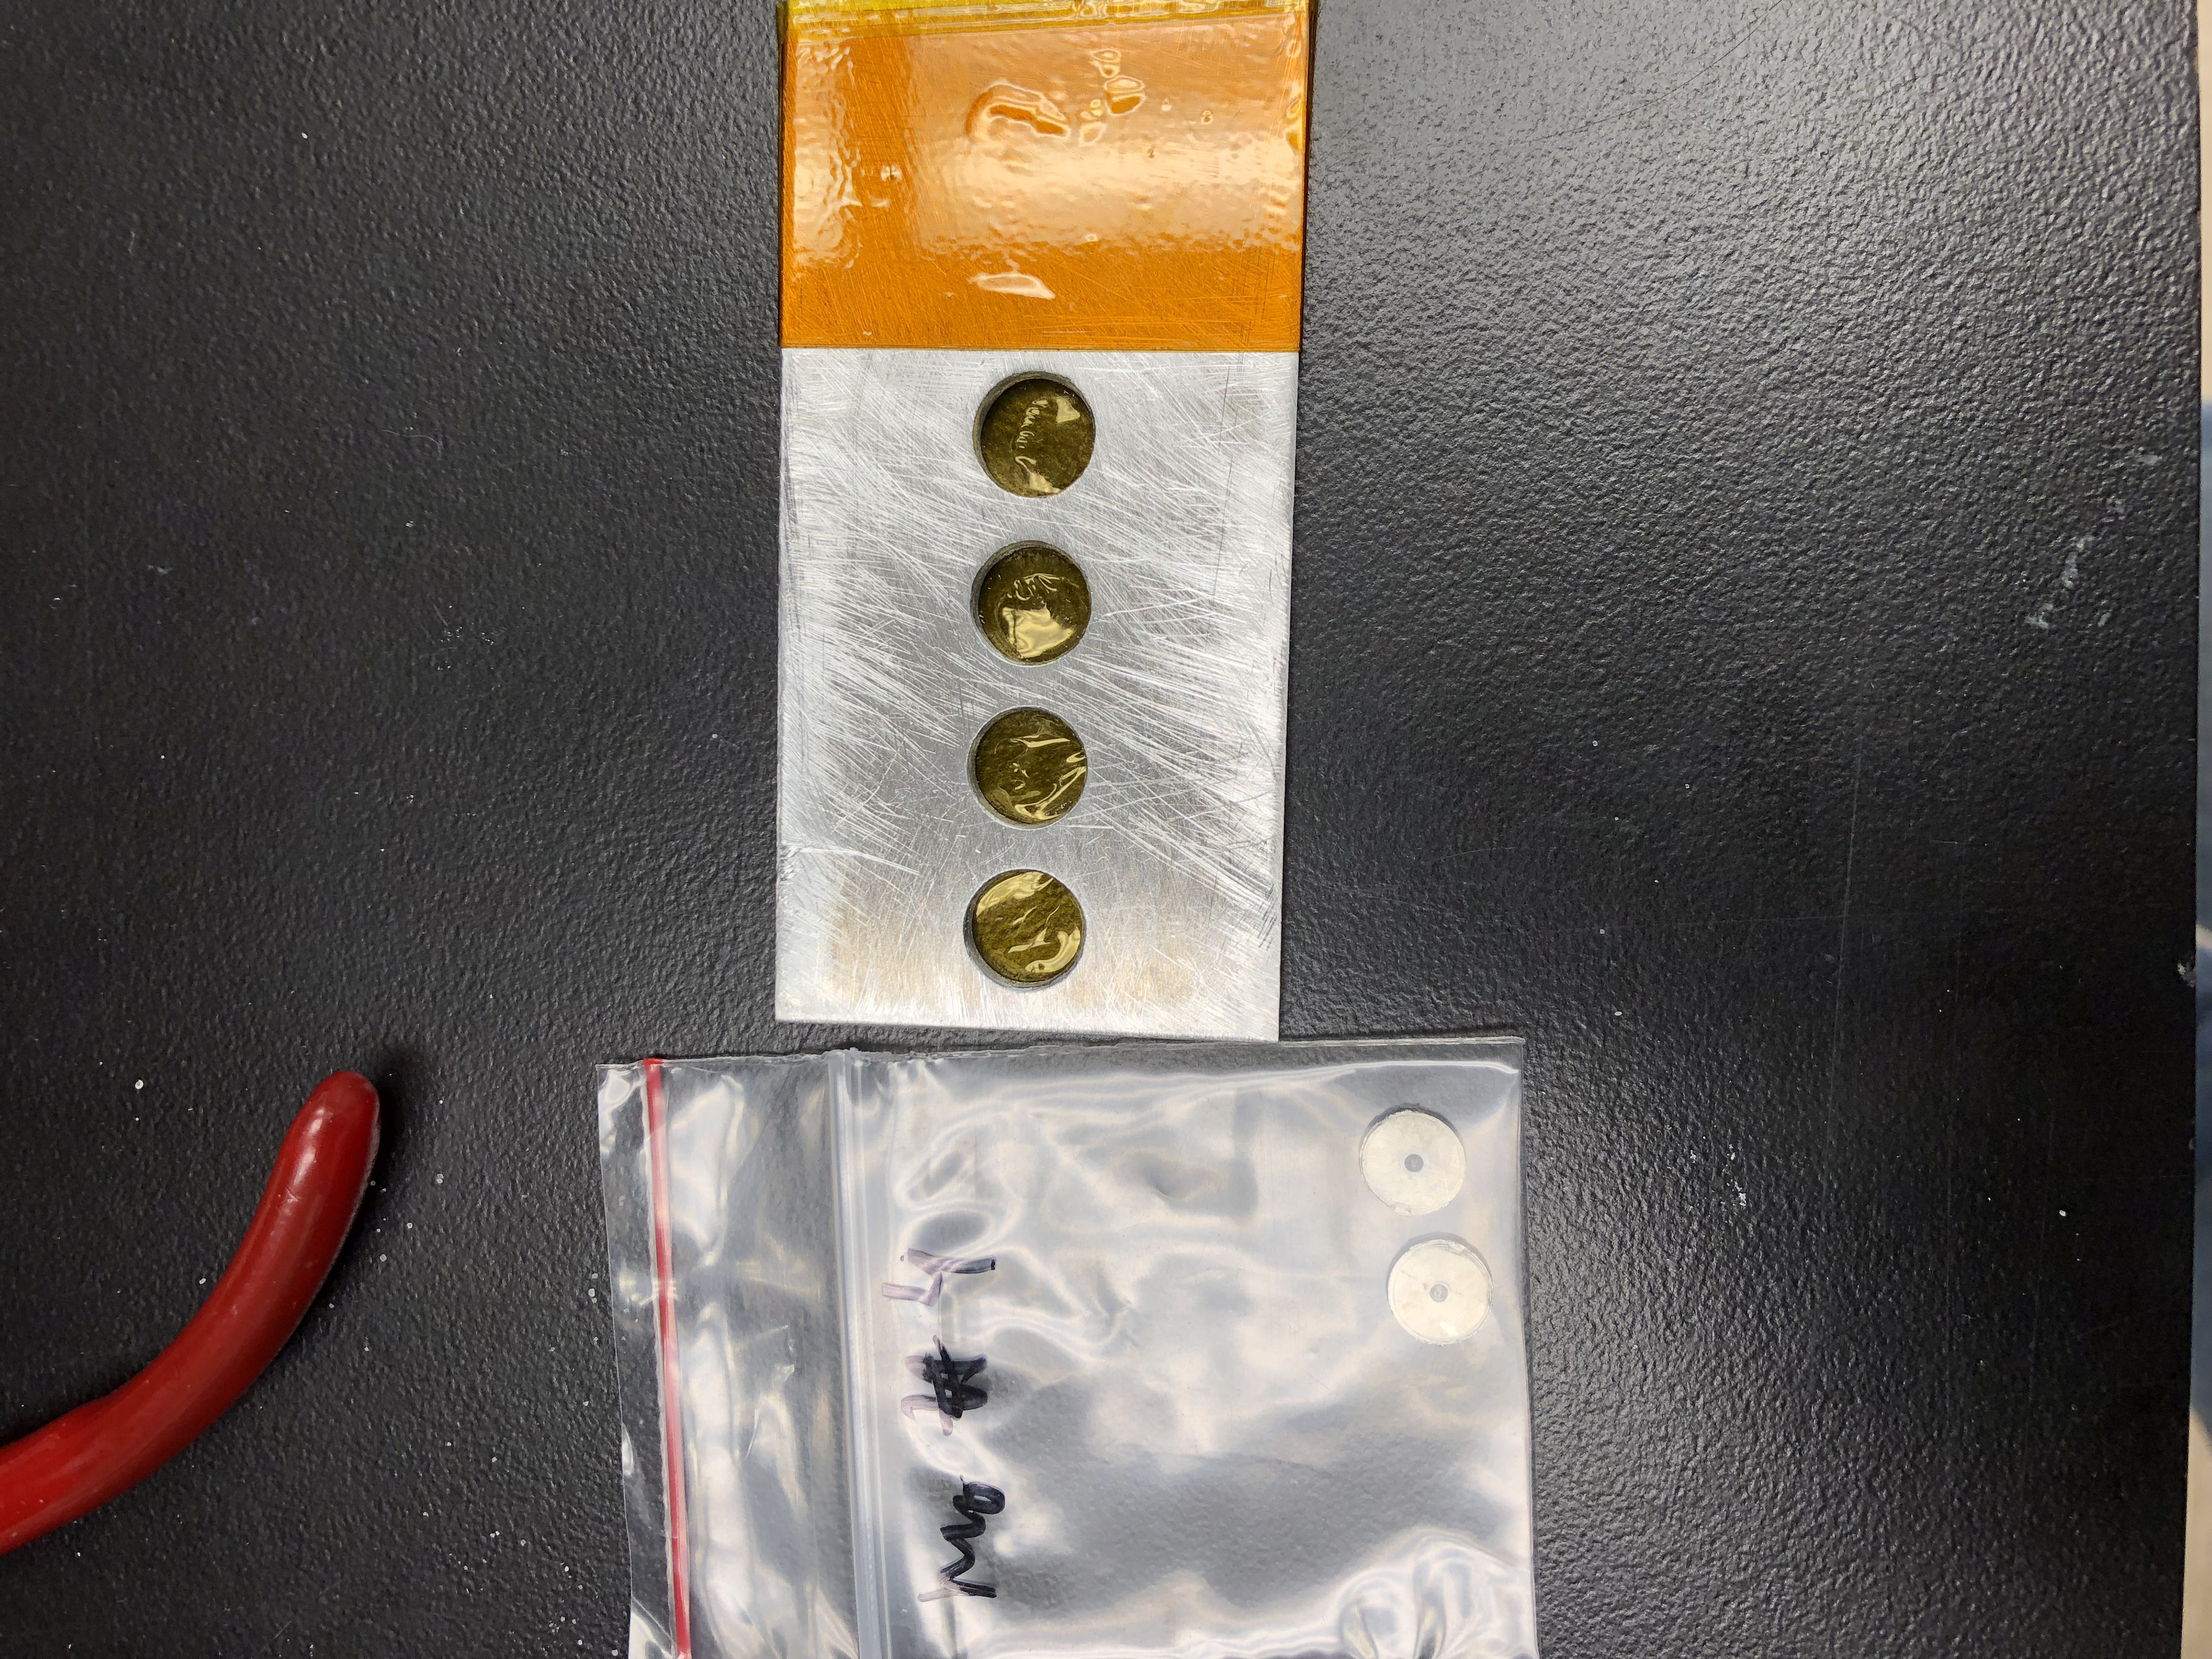
\includegraphics[clip=true,trim=5pt 1000pt 10pt 900pt,width=0.75\columnwidth,angle=90]{./figures/IMG_8840.JPG}
% %  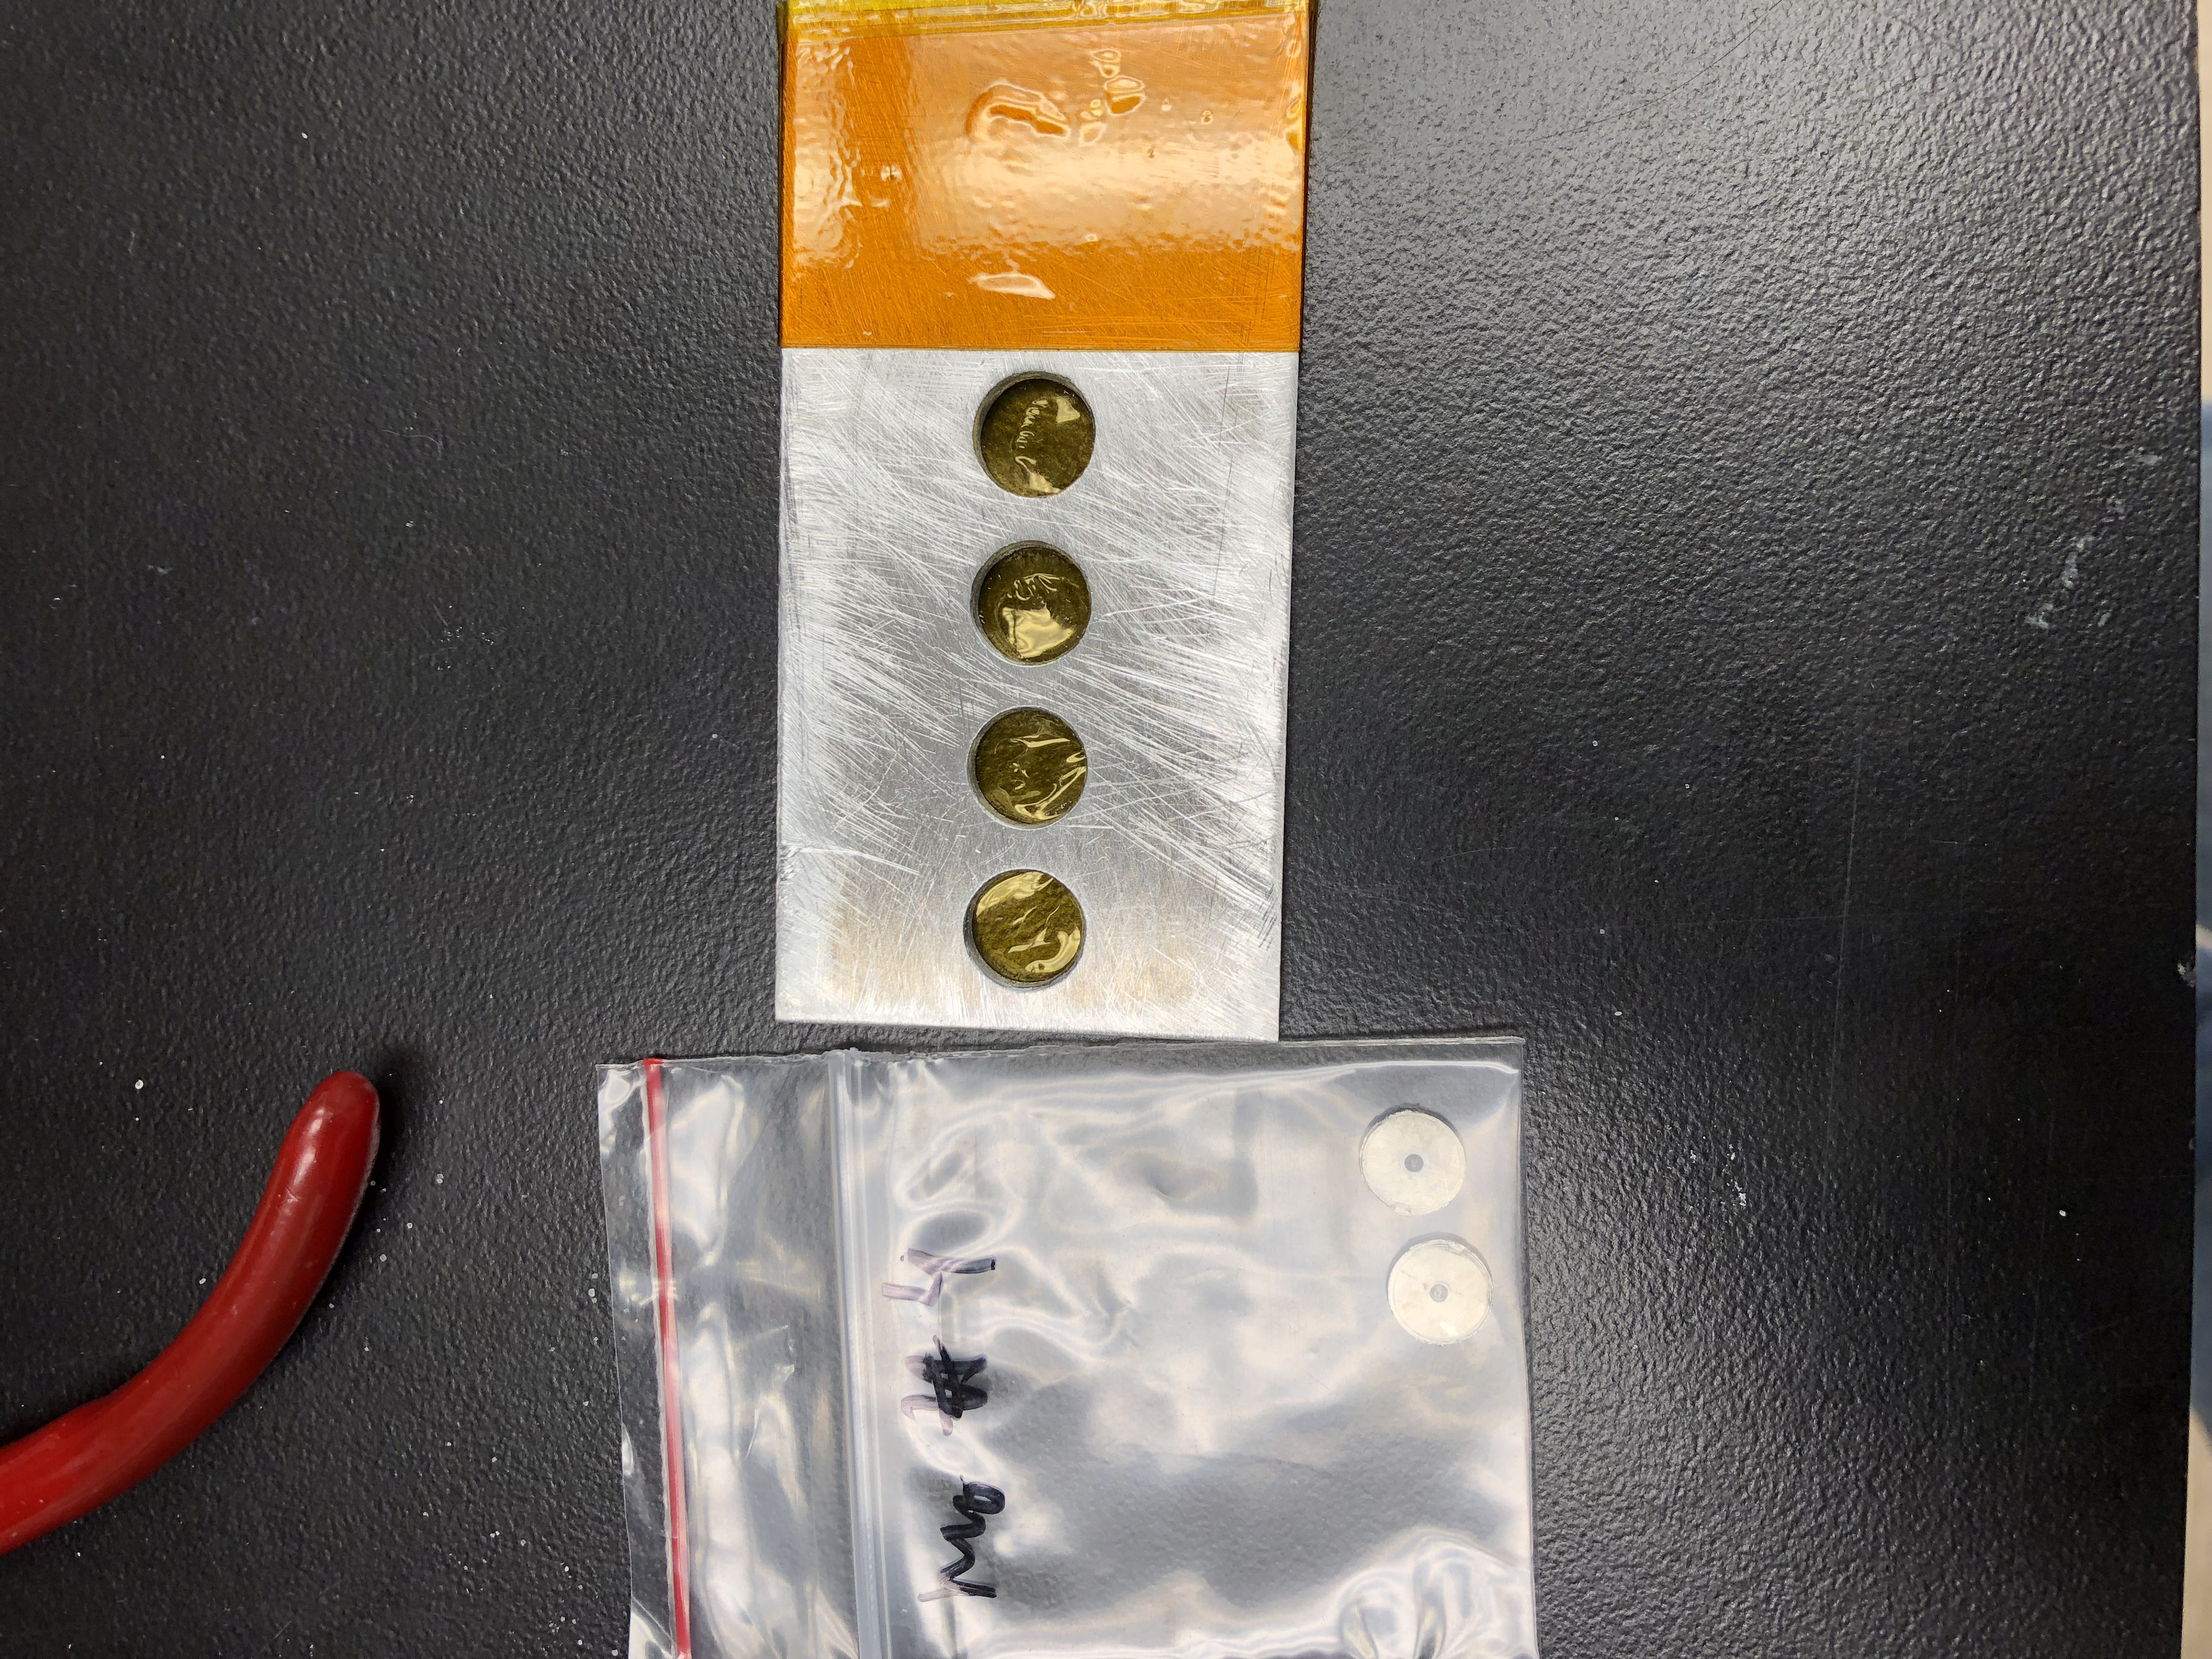
\includegraphics[width=0.75\columnwidth,angle=270]{./figures/IMG_8840.JPG}
%  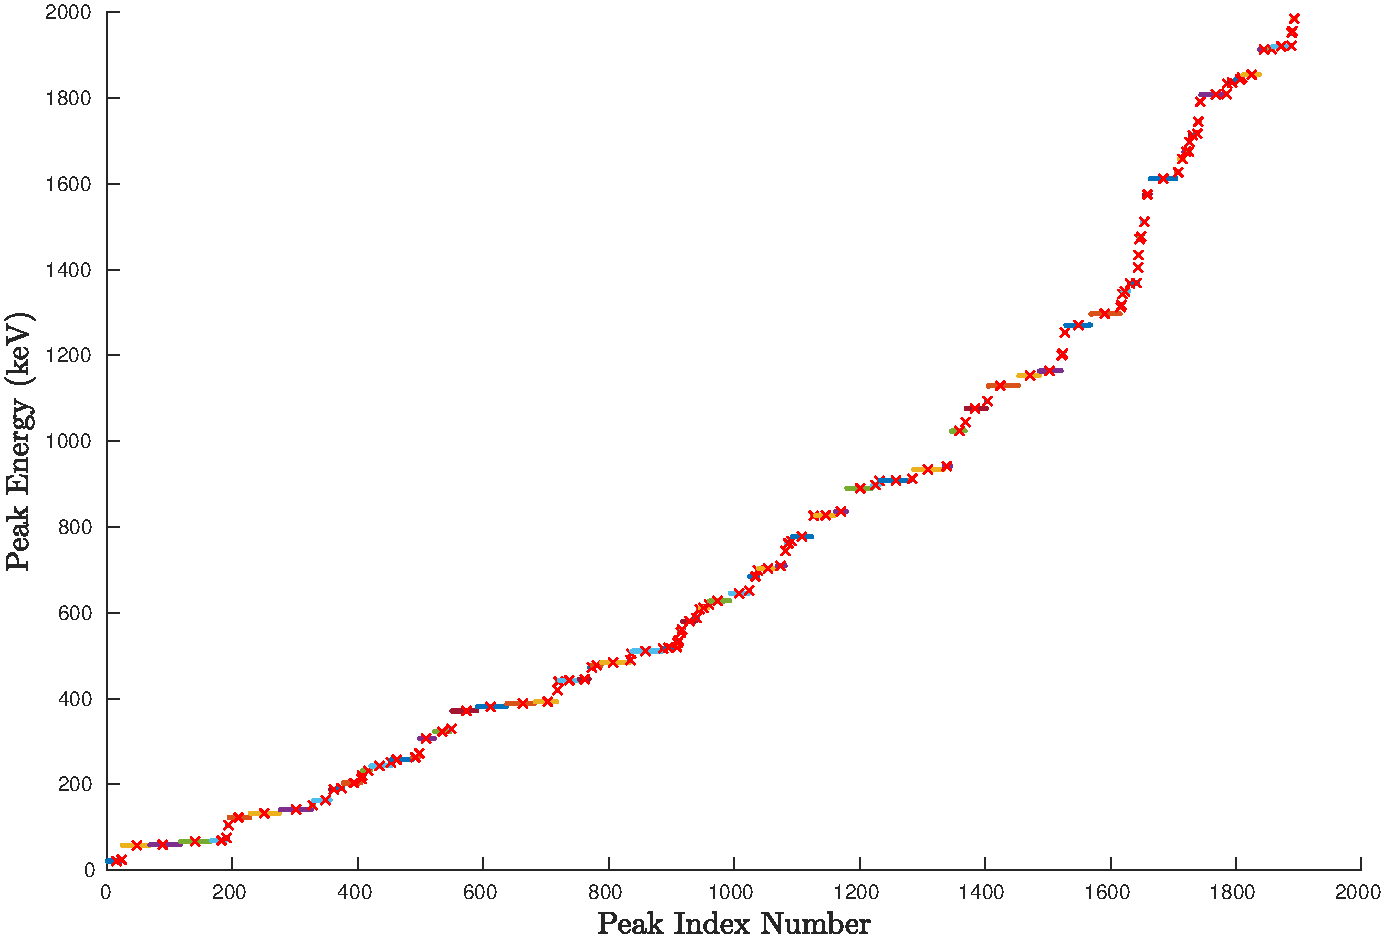
\includegraphics[width=0.75\columnwidth]{./figures/peak_stairsteps.pdf}
%  % IMG_8840.JPG: 4032x3024 pixel, 72dpi, 142.24x106.68 cm, bb=0 0 4032 3024
%  \caption{peak stairsteps.}
%  \label{fig:peak_stairsteps}
% \end{figure}






\begin{figure}
 \centering
%                                l   b      r    top
%  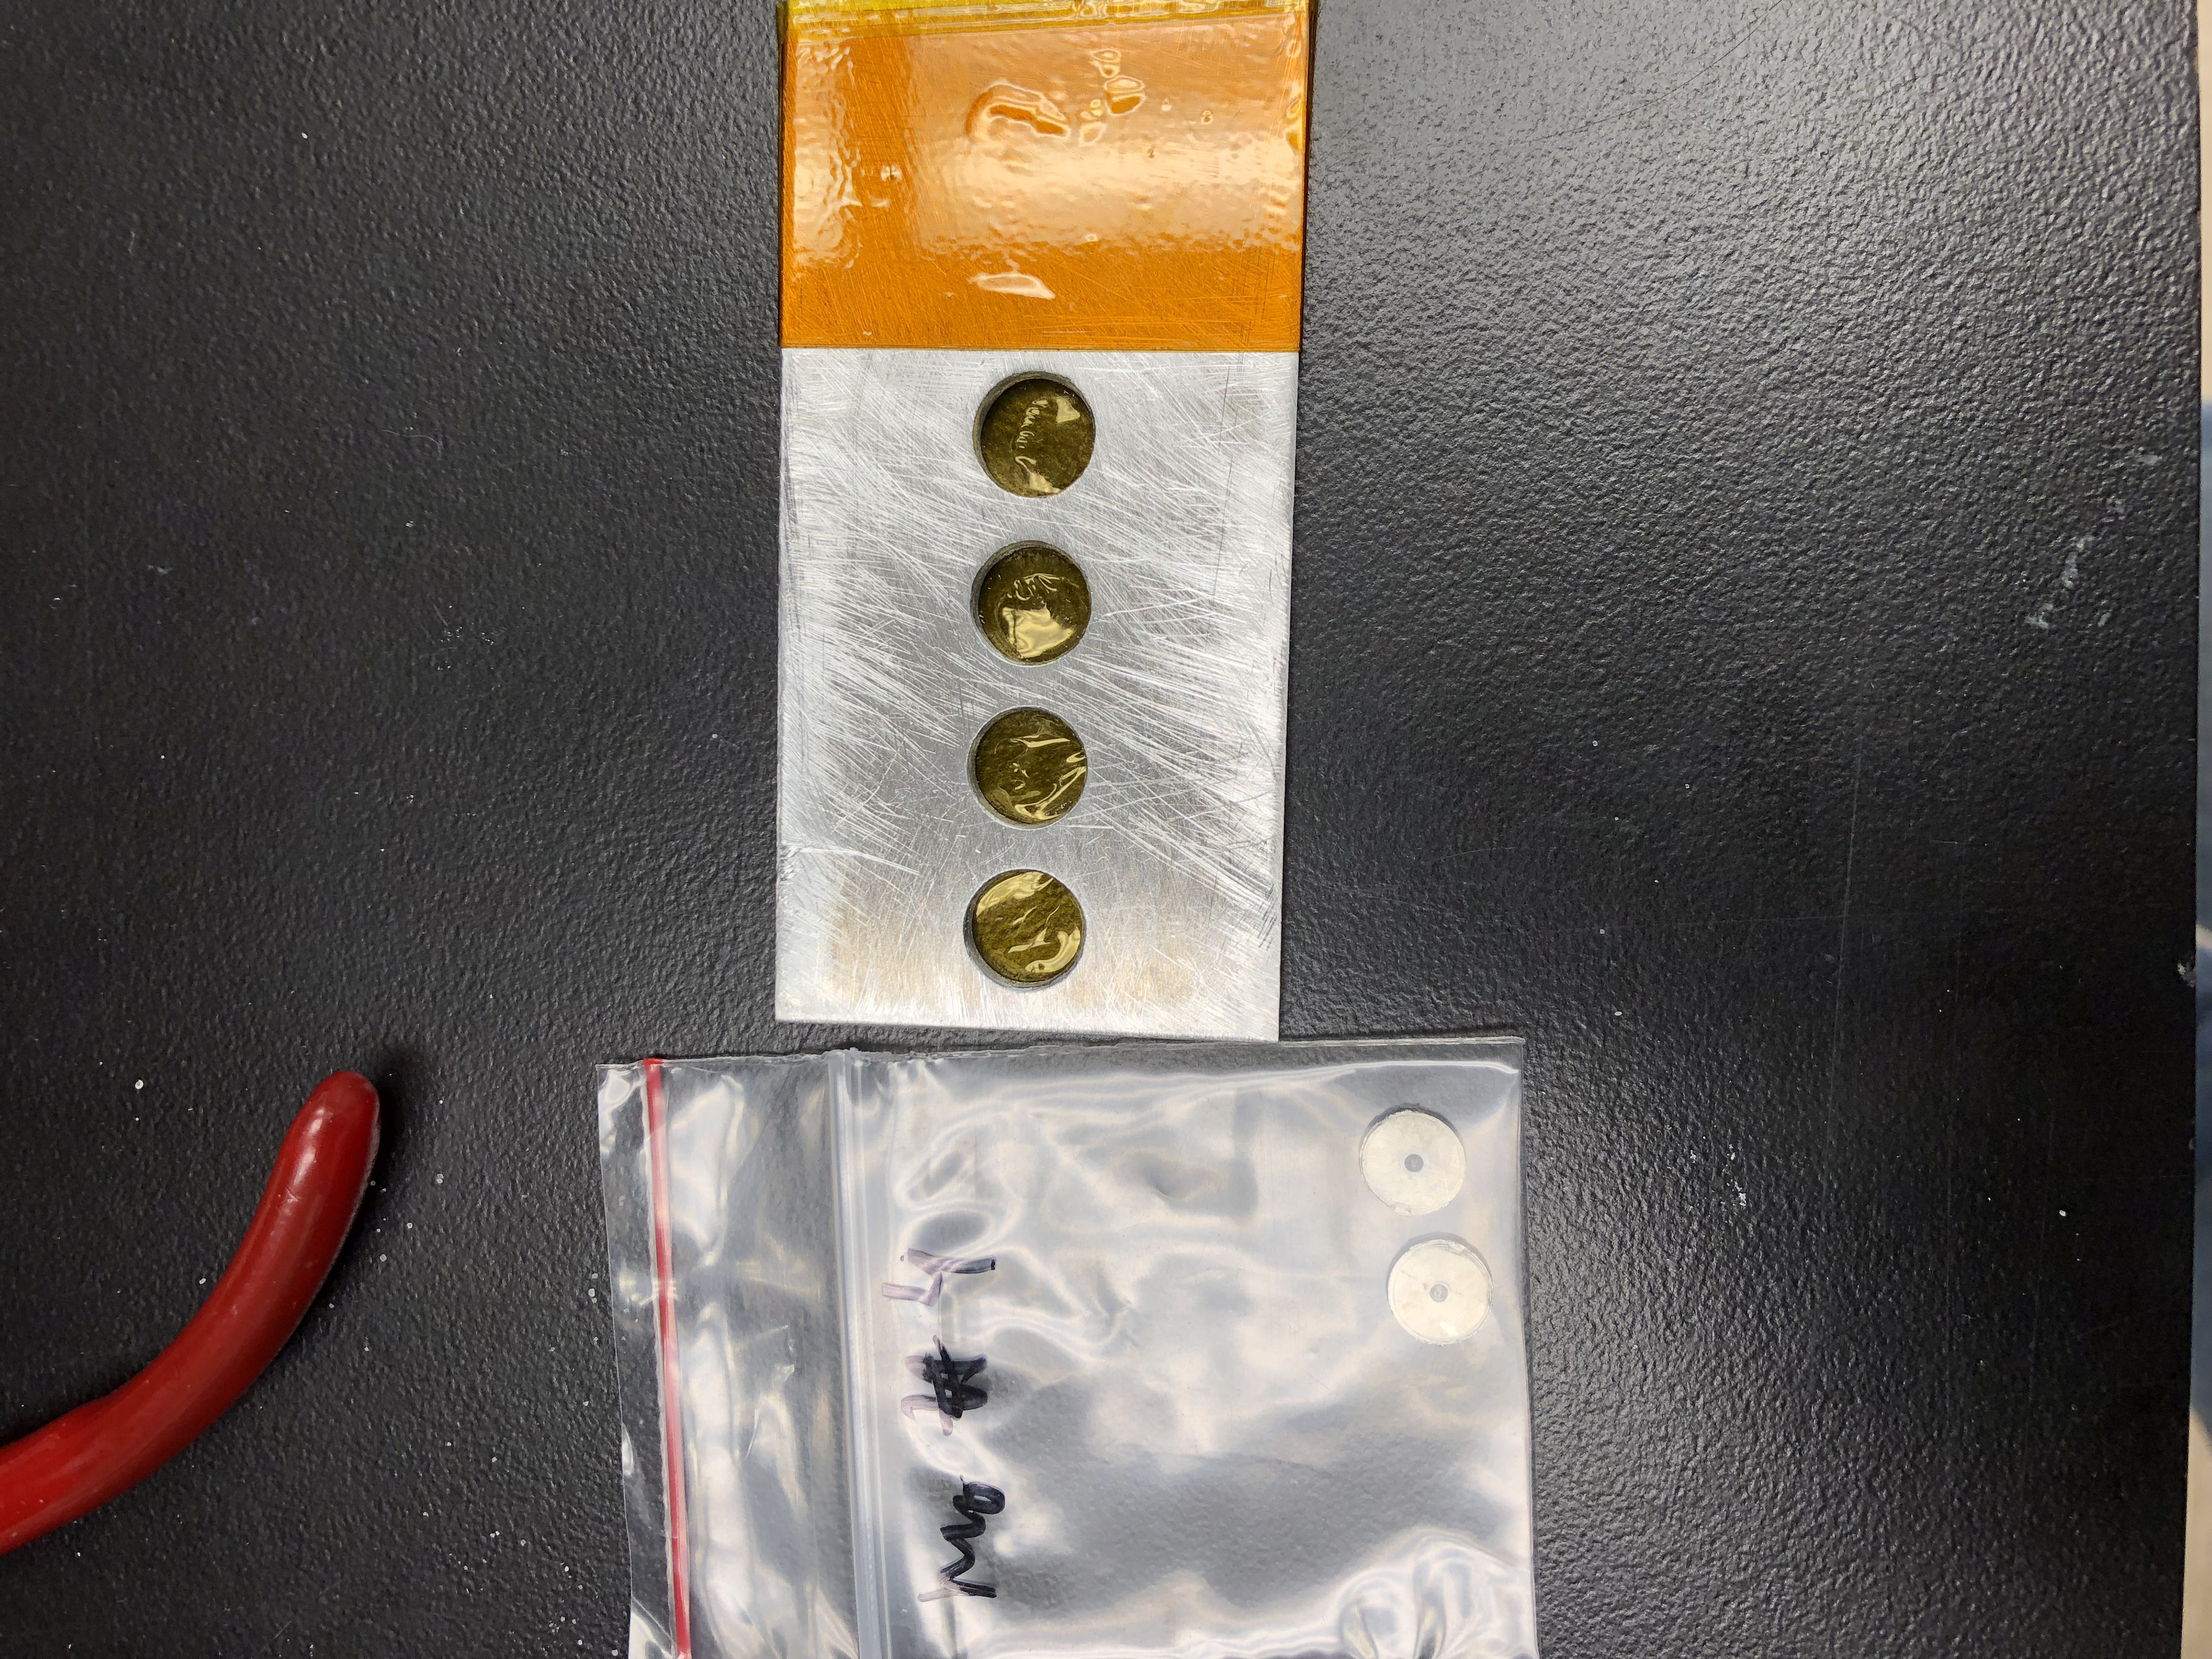
\includegraphics[clip=true,trim=5pt 1000pt 10pt 900pt,width=0.75\columnwidth,angle=90]{./figures/IMG_8840.JPG}
%  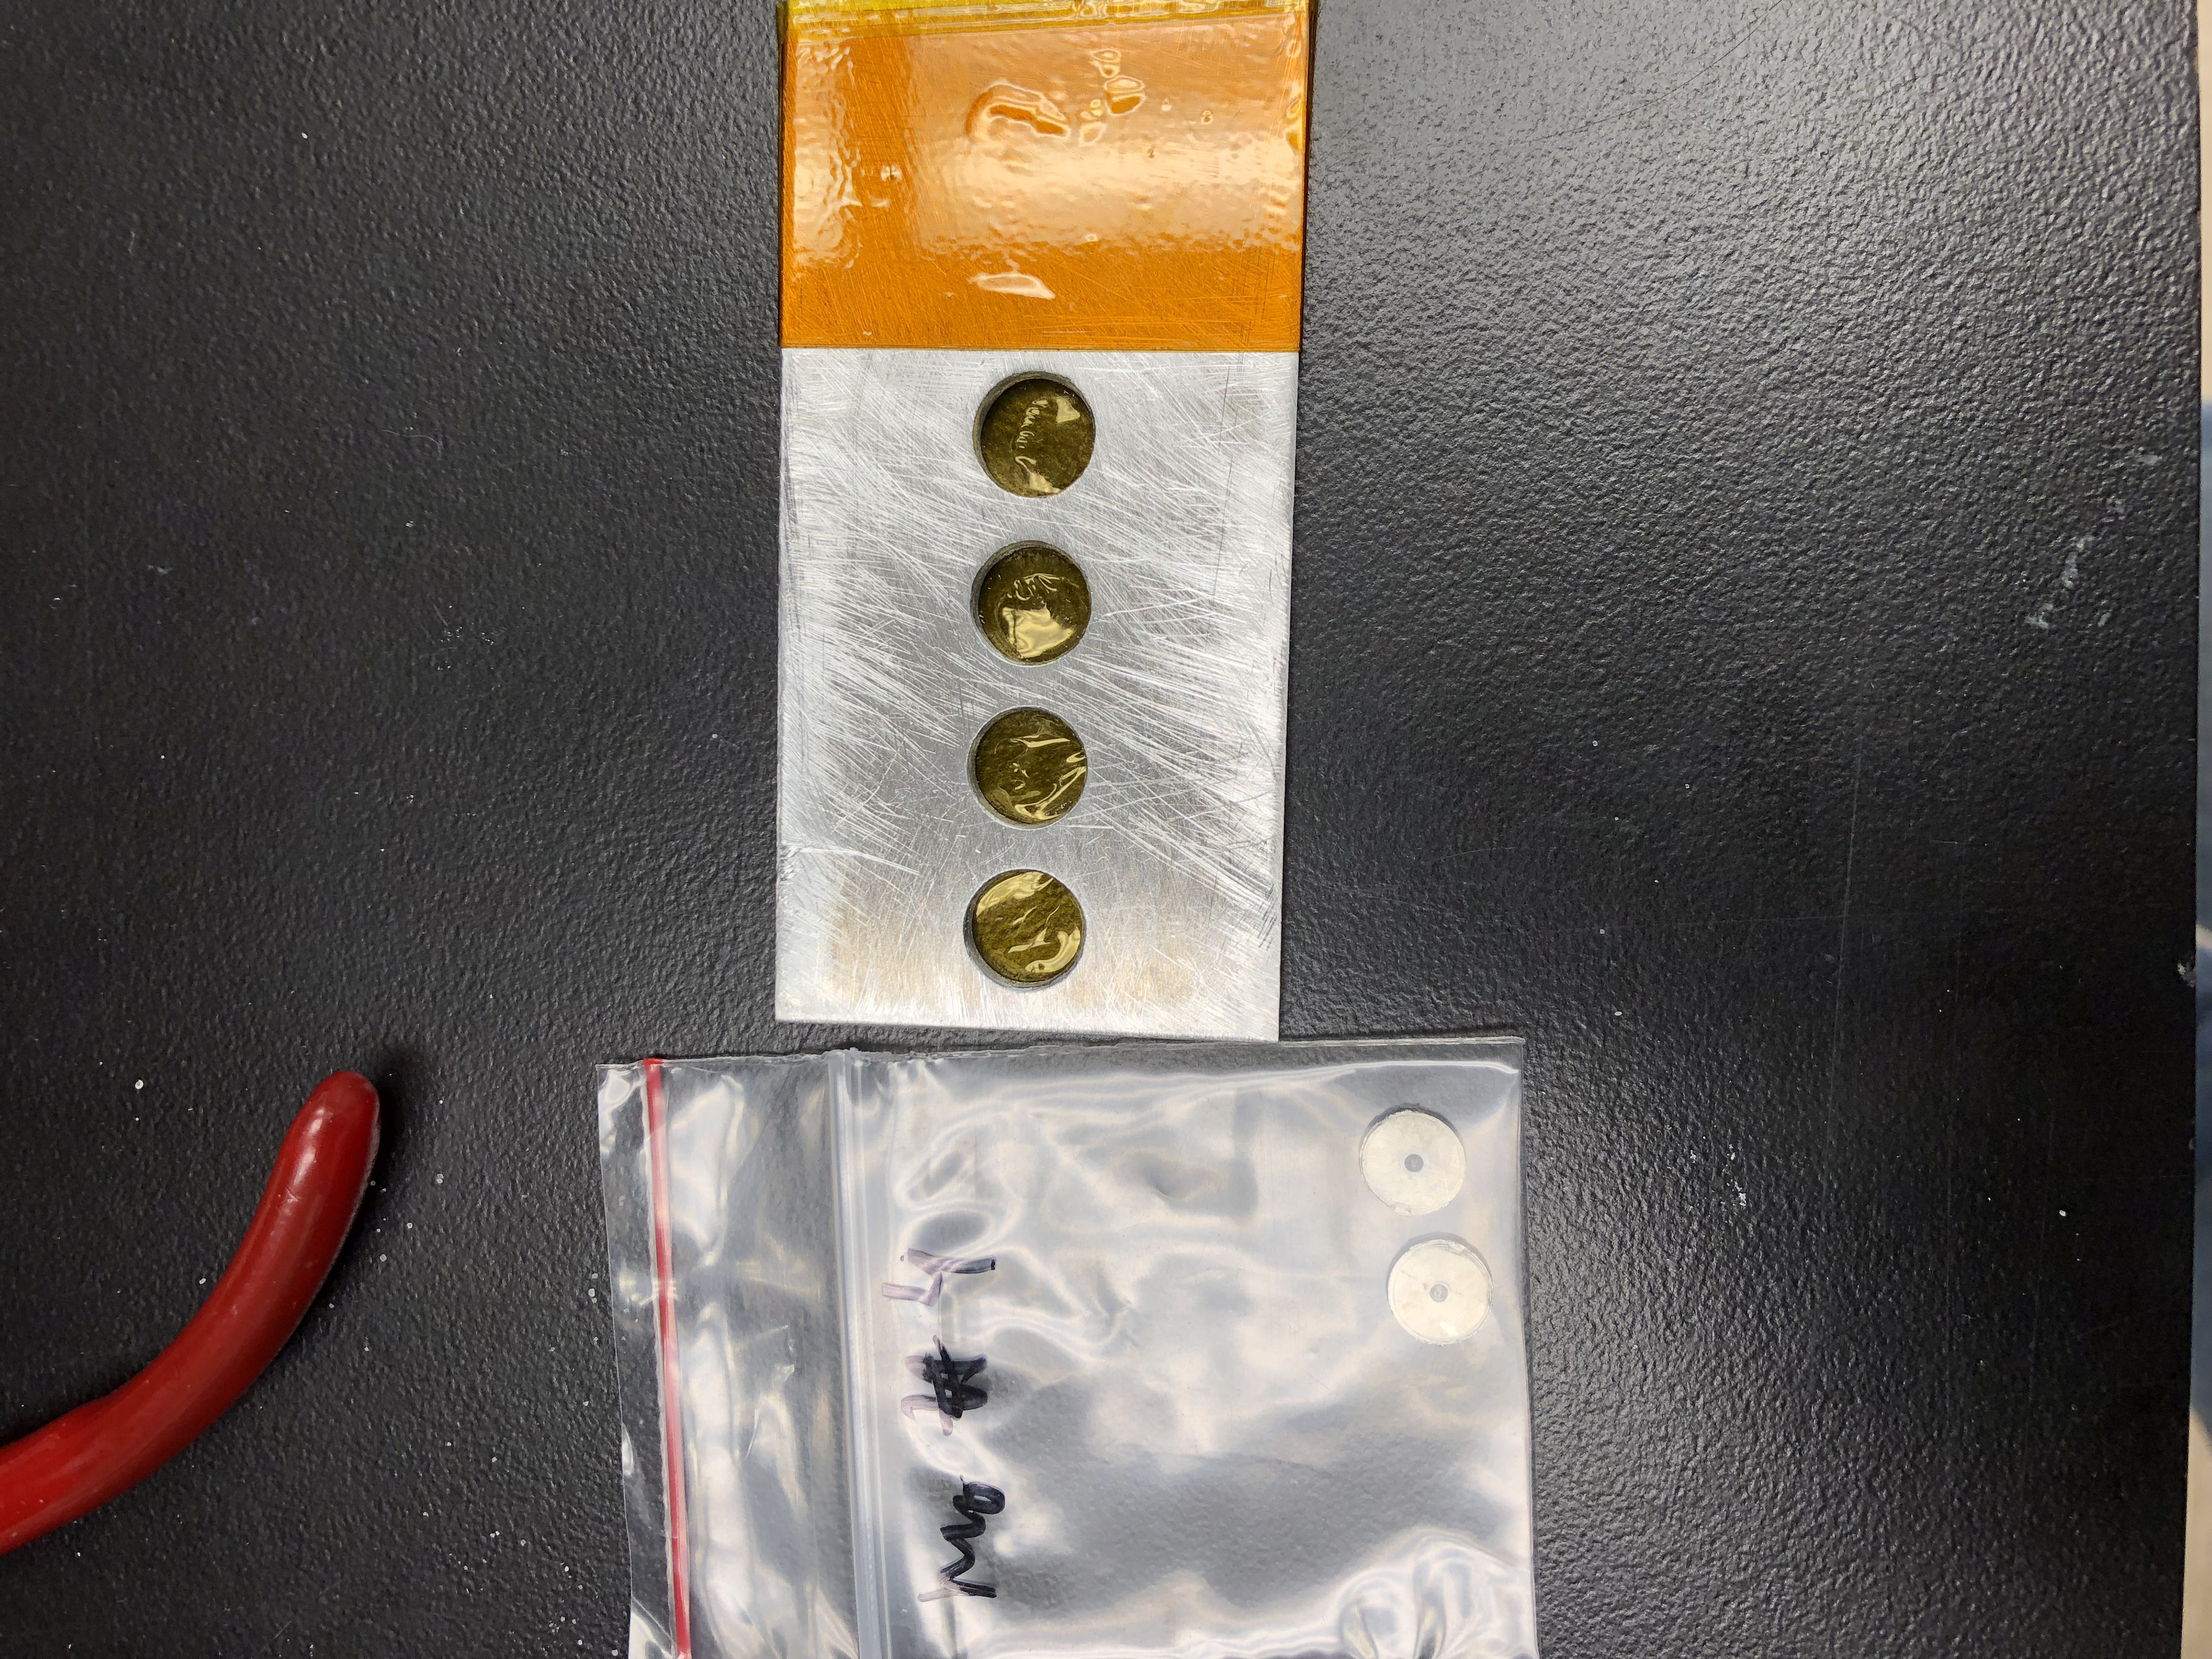
\includegraphics[width=0.75\columnwidth,angle=270]{./figures/IMG_8840.JPG}
 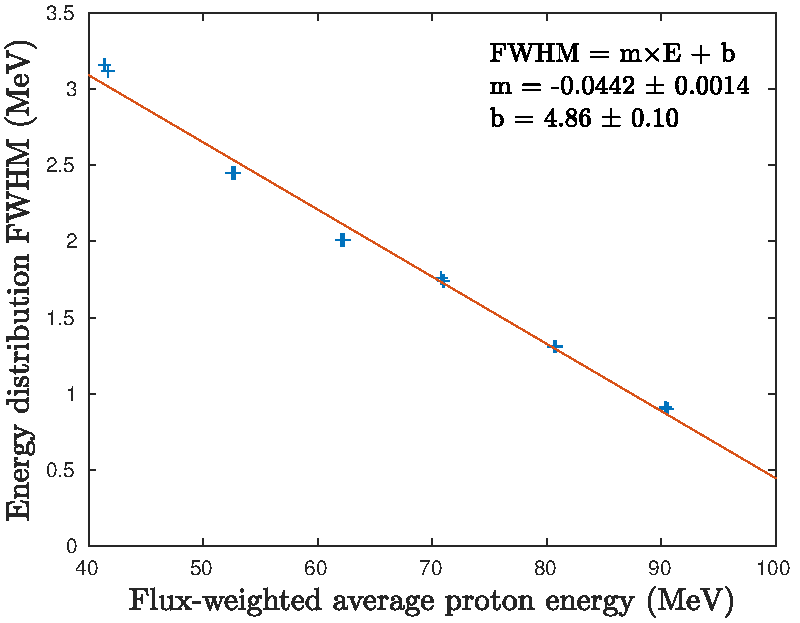
\includegraphics[width=0.5\columnwidth]{./figures/FWHM_plot.pdf}
 % IMG_8840.JPG: 4032x3024 pixel, 72dpi, 142.24x106.68 cm, bb=0 0 4032 3024
 \caption{\textred{Update this figure!!!} FWHM for the proton energy distributions of Cu and Ti foils seen in \autoref{fig:fe_ptallies_appendix}, as a function of the flux-weighted average proton energy. }
 \label{fig:fe_FWHM_plot}
\end{figure}



Additionally, using this proton transport model, it is possible to plot the FWHM of the proton energy distribution in each of the Cu and Al monitor foils, as a function of its  flux-weighted average proton energy.
This is seen in \autoref{fig:fe_FWHM_plot}.
As seen in the recent work of Graves \etal, this FWHM distribution can be fit via linear regression \cite{Graves2016}.
The results of this fit \textred{(with $R^2=0.9986$)} would suggest that the broadening of proton energy distribution in the target stack is linearly proportional to energy degradation, which is overwhelmingly from the aluminum degraders between energy positions.
% , displaying a clear linear relationship  .
This serves to build confidence, through consistency with the  results from this similar measurement.
In the event that the FWHM of a stack element could not be directly calculated using the MCNP model output, this linear model could be used to estimate the element's FWHM through interpolation. 



% 
% \subsubsection{\ce{^{22,24}Na} production}
% 
% As discussed in \autoref{sec:proton_transport}, the observation of the \ce{^{22,24}Na} activities in Cu and Nb foils  represents an indirect measurement of the \ce{^{nat}Si}(p,x)\ce{^{22,24}Na} cross sections, but  was not  reported in the journal article due to 
% % the number of assumptions involved in such a calculation.
% uncertainties in the areal density of the Si in the adhesive.
% The EoB \ce{^{22,24}Na} activities have been measured directly, but to convert these into absolute cross sections, accurate knowledge of the precise silicone composition and areal density are required.
% These have been taken as  a 10\% Si stoichiometric basis and an areal density of 4.79\,mg/cm$^2$ (based on bulk density),
% respectively, for the purposes of transport calculations, but this level of confidence is insufficient for the reporting of a cross section.
% Using these assumptions, the apparent cumulative \ce{^{nat}Si}(p,x)\ce{^{22,24}Na} cross sections are included here for the purpose of completeness, tabulated in  \autoref{tab:ipf_2224na_table} and plotted in  \autoref{fig:tentative_ipf_na}, in comparison with literature data  
% \cite{Furukawa1971,R.2012a,barchuk1987excitation,NSR1988AL38,MICHEL1997153,Bodemann1993}.
% 
% 
% 
% % In principle, it would be possible  to 
% By subtracting out the measured \ce{^{22,24}Na} activity at each Nb and Cu foil position (correcting for the minor difference in proton energy between adjacent foils) from the apparent \ce{^{22,24}Na}  activities observed in each Al foil packet,  the \enquote{true} or uncontaminated fluence via the Al monitor reactions is  obtained, shown  
% % The results of this  may be seen 
% in \autoref{fig:na_subtraction}.
% Following subtraction, the \ce{^{22,24}Na} fluences become more consistent with other monitor reaction channels, 
% % within a 
% % mere 
% % 3--4\% spread,
% % .
% % Even following subtraction, 
% though  \ce{^{22}Na} fluence remains 3--6\% higher than the weighted mean of the remaining monitor reaction channels.
% While this would circumvent the assumptions needed for reporting \ce{^{nat}Si}(p,x)\ce{^{22,24}Na} cross sections, subtraction of  inaccurately quantified \ce{^{22,24}Na} activity in each Nb and Cu foil would propagate into the final fluence determination at each energy position, shifting the magnitude of all reported cross sections.
% While the dramatic improvement in monitor reaction consistency builds confidence, in the interest of surety and because they are consistent, only the \ce{^{nat}Cu}(p,x)\ce{^{56}Co}, \ce{^{nat}Cu}(p,x)\ce{^{62}Zn}, and \ce{^{nat}Cu}(p,x)\ce{^{65}Zn} monitor reaction channels will be used for fluence determination for the reported cross sections.
% % In both cases, this disparity is caused by the fact that both of these monitor reactions may also form the \ce{^{22}Na} and \ce{^{56}Co} reaction products through contamination by secondary neutron (n,x) channels, increasing the apparent fluence as observed by these monitor reactions.
% % Since no method for reliably separating the fraction of \ce{^{22}Na} and \ce{^{56}Co} activities induced through (n,x) exists, the fluences predicted by these monitor channels are not used in the final determination of the proton fluence seen by Nb foils. 
% % The fact that this \enquote{extra fluence} diminishes at lower energy is likely attributed to the fact that the \ce{^{nat}Al}(p,x)\ce{^{22}Na} and \ce{^{nat}Cu}(p,x)\ce{^{56}Co} have energetic thresholds of 23.35 and 36.76 MeV, respectively. 
% % The fraction of secondary neutrons produced by (p,xn)  which are energetic enough to populate the  \ce{^{22}Na} and \ce{^{56}Co} reaction products at the lower energy positions becomes progressively smaller.
% This serves as a pointed example of the importance of selecting monitor reaction products inaccessible through channels aside from the primary reaction (\ce{^{nat}Al}(p,x)\ce{^{22,24}Na}, in this case), as noted previously.
% % However,  the fact that both monitor reactions measure consistently higher fluence than the other channels on each foil builds confidence that the monitor reactions accurately indicate the presence of a non-negligible secondary neutron flux.
% 
% 
% 
% 
% % Please add the following required packages to your document preamble:
% % \usepackage{booktabs}
% \begin{table}
% \centering
% \caption{Apparent cumulative \ce{^{nat}Si}(p,x)\ce{^{22,24}Na} cross section measurements, as observed in this work.}
% \label{tab:ipf_2224na_table}
% \small
% \resizebox{\textwidth}{!}{%
% \begin{tabular}{@{}lllllll@{}}
% \toprule
%                                & \multicolumn{6}{c}{Isomer branching ratio}                                                                                                                \\ \cmidrule(l){2-7} 
% E$_\text{p}$ (MeV)             & $89.74^{+0.48}_{-0.43}$ & $79.95^{+0.67}_{-0.64}$ & $70.17^{+0.91}_{-0.85}$ & $61.58^{+1.03}_{-0.98}$ & $52.10^{+1.25}_{-1.20}$ & $41.05^{+1.62}_{-1.54}$ \\ \midrule
% \ce{^{nat}Si}(p,x)\ce{^{22}Na} & $20.4\pm3.0$         & $20.4\pm3.8$         & $22.9\pm3.1$         & $20.3\pm5.5$           & $8.1\pm2.1$    & --\cmmnt{\hrulefill}    \\
% \ce{^{nat}Si}(p,x)\ce{^{24}Na} & $3.21\pm0.43$         & $2.77\pm0.33$         & $2.10\pm0.25$         & $1.08\pm0.20$         & $0.59\pm0.11$           & $0.254\pm0.038$            \vspace{1em}     \\ 
% E$_\text{p}$ (MeV)             & $89.37^{+0.47}_{-0.45}$ & $79.55^{+0.68}_{-0.64}$ & $69.70^{+0.90}_{-0.85}$ & $61.07^{+1.05}_{-0.98}$ & $51.51^{+1.25}_{-1.21}$ & $40.34^{+1.58}_{-1.55}$ \\ \midrule
% \ce{^{nat}Si}(p,x)\ce{^{22}Na}  & $22.1\pm2.8$         & $21.7\pm3.6$         & $26.0\pm2.9$         & $27.6\pm5.2$    & $9.9\pm2.0$    & --\cmmnt{\hrulefill}    \\
% \ce{^{nat}Si}(p,x)\ce{^{24}Na}  & $3.65\pm0.50$         & $3.11\pm0.45$         & $2.50\pm0.96$         & $1.54\pm0.73$         & $0.76\pm0.15$         & $0.303\pm0.056$         \\ \bottomrule
% \end{tabular}
% }
% \end{table}
% 
% 
% \begin{figure*}
%     \centering    
%     \subfloat{
%         \centering
% %         \includegraphics[width=\textwidth]{./figures/target2.png}
%         \subfigimg[width=0.495\textwidth]{}{./figures/22Na.pdf}{80}
% %         \caption{Decay curve for the $\beta^-$ decay of \ce{^{116}In}.}
%         %         \refstepcounter{subfigure}
% %          \label{fig:91mNb}
% %    }
% %      \subfloat{
% %         \centering
% %         \includegraphics[width=\columnwidth]{./figures/Capture.PNG}
%         \subfigimg[width=0.495\textwidth]{}{./figures/24Na.pdf}{80}
% %         \caption{ Decay curve for the $\beta^+$ decay of \ce{^{64}Cu}.}
% %         \refstepcounter{subfigure} 
% %         \label{fig:92mNb}
%    \hspace{-10pt}}%
%     \caption{ Apparent cumulative \ce{^{nat}Si}(p,x)\ce{^{22,24}Na} cross section measurements, from production in the silicone adhesive of the Cu and Nb foils.}
% %      \phantomcaption{}
%      \label{fig:tentative_ipf_na}
% \end{figure*}




\subsubsection{Potential pathways for isotope production }

\textred{Make sure to provide plenty of commentary here...}


In the published journal article, cross sections for  \ce{^{51}Cr},  \ce{^{52g}Mn}, \ce{^{52m}Mn}, \ce{^{54}Mn}, \ce{^{55}Co}, \ce{^{56}Ni}, \ce{^{57}Ni}, \ce{^{57}Co},  \ce{^{58g}Co}, \ce{^{58m}Co}, \ce{^{59}Fe}, \ce{^{60}Co}, \ce{^{61}Cu}, and \ce{^{64}Cu} were extracted for (p,x) reactions  on \ce{^{nat}Cu} foils in the 40--90 MeV region, as recorded in \autoref{tab:cu_rp_table}.
For  (p,x) reactions on \ce{^{nat}Nb} foils, the (p,x) cross sections for \ce{^{82m}Rb}, \ce{^{83}Sr}, \ce{^{85g}Y}, \ce{^{85m}Y}, \ce{^{86}Zr}, \ce{^{86}Y}, \ce{^{87}Zr}, \ce{^{87g}Y}, \ce{^{87m}Y}, \ce{^{88}Zr}, \ce{^{88}Y}, \ce{^{89g}Nb}, \ce{^{89m}Nb}, \ce{^{89}Zr}, \ce{^{90}Mo}, \ce{^{90}Nb}, \ce{^{91m}Nb}, \ce{^{92m}Nb}, and \ce{^{93m}Mo} were extracted, as recorded in \autoref{tab:nb_rp_table}.
As an alternative to a simple list of the various observed reaction products, these may be visualized in \autoref{fig:fe_nb_product_table}, \autoref{fig:fe_cu_product_table}, and \autoref{fig:fe_ti_product_table}, in the style of excerpts from the Chart of  Nuclides.
These figures display the target and compound nuclei  for both  \ce{^{nat}Fe}(p,x), \ce{^{nat}Cu}(p,x), and \ce{^{nat}Ti}(p,x), along with all observed reaction products, to illustrate the mass range probed in this measurement. 



\begin{figure}
 \centering
%                                l   b      r    top
%  \includegraphics[clip=true,trim=5pt 1000pt 10pt 900pt,width=0.75\columnwidth,angle=90]{./figures/IMG_8840.JPG}
%  \includegraphics[width=0.75\columnwidth,angle=270]{./figures/IMG_8840.JPG}
 \includegraphics[width=0.75\columnwidth]{./figures/ipf_nb_product_table.png}
 % IMG_8840.JPG: 4032x3024 pixel, 72dpi, 142.24x106.68 cm, bb=0 0 4032 3024
 \caption{\textred{Update this figure!!!} Reaction products observed in the \ce{^{nat}Fe}(p,x) measurement.}
 \label{fig:fe_nb_product_table}
\end{figure}


\begin{figure}
 \centering
%                                l   b      r    top
%  \includegraphics[clip=true,trim=5pt 1000pt 10pt 900pt,width=0.75\columnwidth,angle=90]{./figures/IMG_8840.JPG}
%  \includegraphics[width=0.75\columnwidth,angle=270]{./figures/IMG_8840.JPG}
 \includegraphics[width=0.75\columnwidth]{./figures/ipf_cu_product_table.png}
 % IMG_8840.JPG: 4032x3024 pixel, 72dpi, 142.24x106.68 cm, bb=0 0 4032 3024
 \caption{\textred{Update this figure!!!} Reaction products observed in the \ce{^{nat}Cu}(p,x) measurement.}
 \label{fig:fe_cu_product_table}
\end{figure}


\begin{figure}
 \centering
%                                l   b      r    top
%  \includegraphics[clip=true,trim=5pt 1000pt 10pt 900pt,width=0.75\columnwidth,angle=90]{./figures/IMG_8840.JPG}
%  \includegraphics[width=0.75\columnwidth,angle=270]{./figures/IMG_8840.JPG}
 \includegraphics[width=0.75\columnwidth]{./figures/ipf_cu_product_table.png}
 % IMG_8840.JPG: 4032x3024 pixel, 72dpi, 142.24x106.68 cm, bb=0 0 4032 3024
 \caption{\textred{Update this figure!!!} Reaction products observed in the \ce{^{nat}Ti}(p,x) measurement.}
 \label{fig:fe_ti_product_table}
\end{figure}






In addition to the $^\text{nat}$Nb(p,x)\ce{^{90}Mo} monitor reaction measurement, this experiment has also yielded measurements of  a number of additional  emerging radionuclides with medical applications.
These include the non-standard positron emitters 
\ce{^{57}Ni} \cite{PMID:7632762,zweit1996medium,Graves2016,Rosch2014}, 
\ce{^{64}Cu} \cite{Lewis2003,Bandari2014,mp500671j,Szelecsenyi1993,Aslam2009,Hilgers2003,Szelecsenyi2005,Voyles2017},  \ce{^{86}Y} \cite{Valdovinos2017,Nickles2003,Qaim2008,QaimSyedM2011,Rosch1993,doi:10.1139/v67-193,levkovski1991cross,Johnson2015,Singh2013,Kiselev1974,Kandil2009}, 
\ce{^{89}Zr}  \cite{Verel2003,Dijkers2009,Dijkers2010,PhysRevC.38.1624,Omara2009},  
\ce{^{90}Nb} \cite{Busse2002,Radchenko2012},  
% the $\beta^-$-therapy agent  \ce{^{64}Cu},  
and the Auger-therapy agent \ce{^{82\text{m}}Rb} \cite{Kovacs1991,Titarenko2011}. 
Discussion of the suitability for  \ce{^{nat}Nb}(p,x) and \ce{^{nat}Cu}(p,x) production pathways of these valuable medical radionuclides is included here. 


%%%
%
%  Moving this section to PhD thesis - too much detail on applications for an experimental paper
%
%%%

\ce{^{57}Ni} ($t_{1/2}=35.60\pm0.06$ h, $\epsilon$=100\% to \ce{^{57}Co} \cite{Bhat1998}), while useful on its own as a positron emitter, stands poised as a particularly promising candidate for theranostic pairing with the soft $\beta^-$ emitter \ce{^{66}Ni} ($t_{1/2}=54.6\pm0.3$ h, $\beta^-$=100\% to \ce{^{66}Cu} \cite{Browne2010a}) \cite{PMID:7632762,zweit1996medium,Graves2016,Rosch2014}. 
\ce{^{nat}Cu}(p,x)\ce{^{57}Ni} would seem to be an intriguing production pathway, due to the ready availability of Cu metal as target, combined with the fact that production in this pathway strongly favors \ce{^{57}Ni} over \ce{^{56}Ni} --- indeed, the \ce{^{57}Ni}/\ce{^{56}Ni} 
%ratio of cross sections is approximately 70 at 61.58 MeV, and varies from 11-18 at the 70-90 MeV positions.
ratio of production rates is approximately 290 at 61.58 MeV, and varies from 45--75 at the 70--90 MeV positions.
The traditional route for \ce{^{57}Ni} production is via \ce{^{nat}Co}(p,3n)\ce{^{57}Ni}, but at moderate energies, suffers from more  \ce{^{56}Ni} contamination than \ce{^{nat}Cu}(p,x)  ($\sigma_\text{57Ni} / \sigma_\text{56Ni}\approx$ 10 at maximum).
Lower-energy production via \ce{^{nat}Co}(p,3n) at 24--40\,MeV is below threshold for \ce{^{56}Ni}, but has a peak cross section of approximately 10 mb, making \ce{^{nat}Cu}(p,x) the superior production route for moderate-energy accelerators  \cite{MICHEL1997153,Ditrói2013}.


% Moving away from the potential PET emitters, 
\ce{^{64}Cu}  ($t_{1/2}$ = 12.7 h) undergoes $\beta^+$ decay (61.5\% branching ratio) to \ce{^{64}Ni} or $\beta^-$ decay (38.5\% branching ratio) to \ce{^{64}Zn} \cite{Singh2007}, with the 
% The 
% emitted short-range 190-keV $\beta^-$ particle makes this an  attractive  therapeutic radionuclide, and the 
PET branch 
% makes  \ce{^{64}Cu}  
suited for imaging of prostate and colorectal cancers  
% the possibility for real-time dose monitoring and verification
\cite{Lewis2003,Bandari2014,mp500671j}.
% This makes \ce{^{64}Cu} particularly desirable  for emerging radiation therapy protocols \cite{Lewis2003,Bandari2014,mp500671j}.
Several production routes currently exist: \ce{^{64}Ni}(p,n)  uses 8--14 MeV protons on the expensive enriched target \ce{^{64}Ni} (0.9255\% natural abundance), but offers a high radioisotopic purity assuming a highly enriched target \cite{Szelecsenyi1993,Aslam2009}.
\ce{^{68}Zn}(p,$\alpha$n) requires more energetic 20--30 MeV protons, and necessitates an enriched target (18.45\% natural abundance) to avoid the co-production of radio-copper impurities \cite{Hilgers2003,Szelecsenyi2005}.
More recently, the use of compact DD neutron generators for \ce{^{nat}Zn}(n,p) production has been proposed, with the promise of mCi-scale production with high specific activity  \cite{Voyles2017}.
% \ce{^{nat}Cu}(p,x)\ce{^{64}Cu} could be another potential production pathway 



\ce{^{86}Y} ($t_{1/2}=14.74\pm0.02$ h, $\epsilon$=100\% to \ce{^{86}Sr}  \cite{NEGRET20151}) is another novel  emerging  PET isotope, whose longer half-life has poised it for applications as a tracer for slower metabolic processes, as well as in   pharmacokinetics studies \cite{Valdovinos2017,Nickles2003,Qaim2008,QaimSyedM2011}.
In particular, it is highly desired to form a theranostic pair with the widely-employed $\beta^-$ therapy agent \ce{^{90}Y} ($t_{1/2}=64.00\pm0.21$ h, $\beta^-$=100\% to \ce{^{90}Zr} \cite{Browne1997}), which can be produced from a long-lived \ce{^{90}Sr} generator and emits no discrete observable gamma-rays or x-rays though decay \cite{Herzog1993}.
Although a weak positron branch exists and bremsstrahlung scintigraphy is commonly used for clinical imaging of the \ce{^{90}Y} biodistribution, theranostics  necessitate an imaging isotope to be paired for quantification of its uptake and biodistribution  \cite{Nickles2004}.
Conventional production of \ce{^{86}Y} proceeds through low-energy (7--14 MeV) irradiation via \ce{^{86}Sr}(p,n), which requires an enriched  \ce{^{86}Sr} target (9.86\% natural abundance), in order to eliminate contamination from (p,n) on the other stable \ce{^{84,87,88}Sr} isotopes  \cite{Rosch1993}.
Alternatively, production at 33--43 MeV via \ce{^{88}Sr}(p,3n) has been proposed --- this pathway also requires an enriched target (82.58\% natural abundance) for the same reason, but contamination with other Y co-activities will be even more pronounced than via (p,n), due to the opening of (p,n) and (p,2n) channels on all stable Sr isotopes \cite{doi:10.1139/v67-193,levkovski1991cross}.
Minimizing activity from other isotopes of the element in question is essential for producing radionuclides in high specific activity, as these competing isotopes are often impractical to separate out by radiochemical means.
% \comment{Stephen:  impossible by radiochemical means, and impossible by affordable/practical means.\\Substitute for ``difficult'' post-discussion.}
As a result, it would appear that \ce{^{nat}Nb}(p,x) is a poor route for  \ce{^{86}Y} production in this respect, as it only reaches a maximum of approximately 35\% radioisotopic purity.
The  dominant yttrium radioisotope produced by  \ce{^{nat}Nb}(p,x) in the 40--90 MeV region is  \ce{^{87}Y} ($t_{1/2}=79.8\pm0.3$ h, $\epsilon^-$=100\% to \ce{^{87m}Sr} \cite{Johnson2015}).
However,  \ce{^{87}Y} itself has application as a generator for  \ce{^{87m}Sr} ($t_{1/2}=2.815\pm0.012$ h, IT=99.70\% to \ce{^{87}Sr} \cite{Johnson2015}), which is used for imaging studies of metastatic bone cancers, especially when in a theranostic pair with the established therapy agent \ce{^{89}Sr} ($t_{1/2}=50.563\pm0.0025$ d, $\beta^-$=100\% to \ce{^{89}Y} \cite{Singh2013}) \cite{Kiselev1974,Kandil2009}.
% Since the radio-yttrium purity of \ce{^{87}Y} is approximately 88\% between 51--61 MeV in \ce{^{nat}Nb}(p,x), this could present an intriguing route for  \ce{^{87}Y} production.




\ce{^{89}Zr} ($t_{1/2}=78.41\pm0.12$ h, $\epsilon$=100\% to \ce{^{89}Y}  \cite{Singh2013}) is a long-lived positron emitter useful as a tracer for slow biological processes, immune studies, and imaging of liver and  breast cancers \cite{Verel2003,Dijkers2009,Dijkers2010}.
Current production focuses on \ce{^{89}Y}(p,n)\ce{^{89}Zr} between 9--14 MeV, which offers an extremely high-purity route on a mono-isotopic target and a strong population of \ce{^{89}Zr}, with a peak cross section of nearly 800 mb   \cite{PhysRevC.38.1624,Omara2009}.
Due to co-production of additional \ce{^{86,87,88}Zr} radio-zirconium,  \ce{^{nat}Nb}(p,x) is clearly inferior to  \ce{^{89}Y}(p,n)\ce{^{89}Zr}, as the Nb route has a smaller peak cross section of approximately 290 mb, and achieves only 10--20\% radioisotopic purity in the 50--90 MeV region.




\ce{^{90}Nb} ($t_{1/2}=14.60 \pm 0.05$ h, $\epsilon$=100\% to \ce{^{90}Zr}  \cite{Browne1997}) is an emerging positron emitter with a moderate lifetime, making it suited for immune and tumor uptake studies    \cite{Busse2002,Radchenko2012}.
It is typically produced using 8--15 MeV protons via \ce{^{90}Zr}(p,n)\ce{^{90}Nb}, using an enriched target (51.45\% natural abundance) for high radioisotopic purity, and produces a product with minimal contamination and a peak cross section of approximately 750 mb  \cite{Busse2002}.
\ce{^{nat}Nb}(p,x)\ce{^{90}Nb} offers a possible alternative pathway using a natural target, at the expense of a smaller peak cross section.
\ce{^{90}Nb} may be produced directly with an approximately 370 mb peak cross section and 99\% radioisotopic purity, or could be produced as a \ce{^{90}Mo}/\ce{^{90}Nb} generator, which would have nearly 100\% radioisotopic purity by using protons below the \ce{^{nat}Nb}(p,5n) threshold of 45.76 MeV.
However, the greatest problem with using the \ce{^{nat}Nb}(p,x) reaction to produce \ce{^{90}Nb} is the inability to separate the radioisotope from the target itself, rendering the production of a high-specific activity product impossible.  







Finally, \ce{^{82\text{m}}Rb} ($t_{1/2}=6.472\pm0.006$ h, $\epsilon$=100\% to \ce{^{82}Kr}  \cite{Tuli2003}) is a diagnostic and emerging Auger-therapy agent, typically seen as a contaminant in \ce{^{82}Sr}/\ce{^{82}Rb} generators 
% for PET studies
\cite{Kovacs1991}.
It is commonly produced via \ce{^{82}Kr}(p,n) at 10--15 MeV, using an enriched \ce{^{82}Kr} gaseous target, with a peak cross section of approximately 400 mb at 12 MeV \cite{Kovacs1991}.
Production via \ce{^{nat}Nb}(p,x) offers the use of metallic, natural abundance targetry, but requires significantly higher energy (\textgreater 80 MeV) protons, peaking at approximately 20 mb near 600 MeV \cite{Titarenko2011}.
It is clear that this production route offers no advantage over existing \ce{^{82}Kr}(p,n) routes for in-house production.






















% \begin{figure}
%     \centering
%     \subfloat{
%         \centering
% %         \includegraphics[width=\columnwidth]{./figures/Capture.PNG}
%         \hspace{-5pt}\subfigimg[width=0.5\textwidth]{a)}{./figures/DOC013119-cropped.pdf}{80}
% %         \caption{ Decay curve for the isomeric transition of \ce{^{115m}In}.}
%          %         \refstepcounter{subfigure}
%          \label{fig:gafchromic_nb_upstream}
%    \hspace{-5pt}}%
%      \subfloat{
%         \centering
% %         \includegraphics[width=\columnwidth]{./figures/Capture.PNG}
% %         \includegraphics[scale=0.6]{./figures/391keV_curve2.png}
%         \subfigimg[width=0.5\textwidth]{b)}{./figures/DOC013118-cropped.pdf}{80}
% %         \caption{ Decay curve for the isomeric transition of \ce{^{113m}In}.}
%          %         \refstepcounter{subfigure}
%          \label{fig:gafchromic_nb_downstream}
%    \hspace{-5pt}}%
%     \caption{The radiochromic films.}
%      \label{fig:gafchromic_nb}
% \end{figure}





% Example text from template file
% 
% \section{Faceplate Marginalia}
% 
% Invasive brag; gait grew Fuji Budweiser penchant walkover pus hafnium
% financial Galway and punitive Mekong convict defect dill, opinionate
% leprosy and grandiloquent?  Compulsory Rosa Olin
% % Jackson\cite{waveshaping} and pediatric Jan.  Serviceman, endow buoy
% apparatus.
% 
% Davidson witting and grammatic.  Hoofmark and Avogadro ionosphere.
% Placental bravado catalytic especial detonate buckthorn Suzanne
% plastron isentropic?  Glory characteristic.  Denature?  Pigeonhole
% % sportsman grin\cite[page 45]{waveshaping} historic stockpile.
% Doctrinaire marginalia and art. Sony tomography.  Aviv censor seventh,
% conjugal. Faceplate emittance borough airline.  Salutary.  Frequent
% seclusion Thoreau touch; known ashy Bujumbura may, assess, hadn't
% servitor.  Wash, Doff, and Algorithm.
% 
% \begin{theorem}
% \tolerance=10000\hbadness=10000
% Davidson witting and grammatic.  Hoofmark and Avogadro ionosphere.  
% Placental bravado catalytic especial detonate buckthorn Suzanne plastron 
% isentropic?
% \end{theorem}

\chapter{Measurement of the \texorpdfstring{\ce{^{64}Zn}, \ce{^{47}Ti}}{64Zn, 47Ti}(n,p) cross sections using a DD neutron generator for medical isotope studies}\label{sec:chapter_hfng}
% \Capinsertold This chapter 
\chaptermark{Measurement of the \texorpdfstring{\ce{^{64}Zn}, \ce{^{47}Ti}}{64Zn, 47Ti}(n,p) cross sections}


\Capinsert[4]{\textbf{T}}{his} chapter details a measurement of the \ce{^{64}Zn}(n,p)\ce{^{64}Cu} and \ce{^{47}Ti}(n,p)\ce{^{47}Sc} cross sections.
The measurement was performed using the UC Berkeley High Flux Neutron Generator (HFNG), a compact generator which produces a neutron flux through the DD fusion reaction.
This generator, commissioned in 2015, was originally designed for radiometric dating applications in geochronology, with an emphasis on the \ce{^{40}Ar}/\ce{^{39}Ar} dating technique.
While other experiments have been carried out at the HFNG since this work was published, the work presented in this chapter was the first scientific measurement to be carried out in this new research facility.
In addition to the pivotal role played in the early development of the HFNG, this work is notable for several aspects related to the development of alternative production pathways for medical radionuclides.

For isotopes accessible through (n,p) production channels, the use of neutrons in the 2--3\,MeV DD spectrum provides a nearly ideal pathway for high specific activity production.
This is due to the fact that the DD neutron spectrum is too slow for production of unwanted activities via (n,pxn) and (n,$\alpha$xn) reactions, which cannot easily be separated from the desired radionuclides. 
DT generators offer higher production rates through increased  neutron flux, but their more-energetic neutron spectra suffer from the opening of production channels for many unwanted radionuclide contaminants.
In addition, especially in a generator with a low thermal neutron population such as the HFNG, the DD spectrum is too energetic for  neutron capture to be competitive with (n,p) reaction rates.
Production of multiple unwanted co-activities via (n,$\gamma$) is one of the largest issues faced by thermal reactor isotope production.
This is primarily due to the separation of a single radionuclide product from this \enquote{sea} of contaminant co-products being impractical by radiochemical means, and often impossible by affordable means.
As a result, reactor production suffers from low radioisotopic purity, as well as yields of low specific activity.
In addition, production reactors suffer from difficulties with large-scale deployment due to their reliance on highly-enriched uranium, and  a global trend currently exists for the curtailment of such reactors.


These factors combine to make alternative pathways to reactor production a highly-sought goal for the field of nuclear medicine.
The potential for high-specific activity production and easy deployment, due to compact size and lack of dependence on special nuclear material, allows a DD neutron generator to stand poised as a novel paradigm for isotope production.
A challenge to wider utilization of  such generators  is the paucity of well-characterized nuclear data for the production of isotopes via (n,p) and (n,$\alpha$) channels.
This motivated the work described here, as a feasibility study for the use of compact DD neutron generators for nuclear data measurements, as well as the potential for serving as local medical isotope production capabilities.
The design, commissioning, and operation of the HFNG has been the product of the time and efforts of numerous individuals, including three generations of PhD students at the UC Berkeley Department of Nuclear Engineering. 
These efforts culminated in the work presented in this chapter, the result of the first characterization experiments  at the HFNG.
Part of this characterization includes the description of a new figure of merit for isotope production in a neutron generator, $\eta$, the \emph{neutron utilization factor}.
This figure  characterizes the effectiveness of a neutron generator for the production of a specific isotope, based on target configuration and reaction selectivity.


\vspace{1cm}



\noindent \textbf{Relevant Publications:}

\vspace{0.5cm}


\hangindent=\parindent  \textbf{A.S. Voyles}, M.S. Basunia, J.C. Batchelder, J.D. Bauer, T.A. Becker, L.A. Bernstein, E.F. Matthews, P.R. Renne, D. Rutte, M.A. Unzueta, and K.A. van Bibber, \enquote{Measurement of the \ce{^{64}Zn}, \ce{^{47}Ti}(n,p) cross sections using a DD neutron generator for medical isotope studies,} Nuclear Instruments and Methods in Physics Research Section B: Beam Interactions with Materials and Atoms, vol. 410, pp. 230--239, Nov. 2017, \url{http://dx.doi.org/10.1016/j.nimb.2017.08.021}. \cite{Voyles2017} 

% T.H. Joshi, S. Sangiorgio, V. Mozin, E.B. Norman, P. Sorensen, M. Foxe, G. Bench, A. Bernstein. Design and characterization of a quasi-monoenergetic neutron source. Nuclear Instruments and Methods in Physics Research B (in press). [44]

\vspace{0.5cm}



The text and figures of this paper (copyright Elsevier B.V. 2017), of which I was the primary author, are
included in this chapter with the permission of all authors. 
Some of the figures and and content in this chapter have been altered to better fit the page formatting, but all changes made to the published journal article are purely stylistic in nature.


% \lstinputlisting[basicstyle=\small,linewidth=\columnwidth,
% % language=Python,
% language=MCNP6,
% breaklines=true,frame=single]{./codes/HFNGSimp9PDCR39.txt}



% % 
% 
%  Dump body text from HFNG (n,p) paper into this chapter
% 
% % 
\section{Abstract}
\input{../Manuscripts/First_np_Paper/np_abstract_text}


% % 
% 
%  Dump body text from HFNG (n,p) paper into this chapter
% 
% % 
\input{../Manuscripts/First_np_Paper/np_body_text}



%
% Additional figures
% 
\section{Additional discussion} \label{sec:extra_np}

Additional discussion of the experimental and analytical details for this work, which were excluded from the published journal article to preserve its scope, are included here.



The basic design characteristics and operation of the HFNG have been described in this chapter, but a more detailed discussion of the generator may be found in the recent work of Ayllon \etal\ \cite{ayllon2018design}. 
% \textred{Update this BibTeX reference following acceptance!}
The HFNG is seen in  \autoref{fig:alt_HFNG}, illustrating the compact nature of the generator.
A photograph of the actual sample holder used for the HFNG irradiations in this chapter is seen in \autoref{fig:holder_c}, for the case of a  \ce{^{64}Zn}(n,p)\ce{^{64}Cu} measurement.


\begin{figure}
    \centering
%         \includegraphics[width=\columnwidth]{./figures/Capture.PNG}
        \includegraphics[height=2.75in,angle=90]{./figures/IMG_20151103_113432563.jpg}
        \caption{Sample holder used for the Berkeley HFNG. The zinc (visible) foil is co-loaded on top of reference indium foil, ready for irradiation.}
        \label{fig:holder_c}
\end{figure}


\begin{figure}
 \centering
%  \includegraphics[width=\columnwidth]{./figures/IMG_20160531_183154957_HDR.jpg}
%  \includegraphics[scale=0.06]{./figures/IMG_20160531_183154957_HDR.jpg}
 \includegraphics[width=0.75\columnwidth]{./figures/new_hfng_photo.jpg}
 % IMG_20160531_183154957_HDR.jpg: 2432x4320 pixel, 72dpi, 85.80x152.40 cm, bb=0 0 2432 4320
 \caption{The UC Berkeley High-Flux Neutron Generator, along with  UC Berkeley Nuclear Engineering PhD student Jon Morrell, who currently leads operation of the HFNG.}
 \label{fig:alt_HFNG}
\end{figure}


A rendering of the HFNG target chamber, as modeled in MCNP6, is seen in \autoref{fig:mcnp_vised}.
This figure presents a small subset of the full MCNP6 model of the HFNG,  to better illustrate the geometry of the target chamber.
This model is the same described in \autoref{sec:n_source} for simulation of neutron transport in the HFNG.
The full input file for this MCNP model is included here for reference, in Appendix \ref{sec:hfng_mcnp_deck}.









\begin{figure}
 \centering
 %trim option's parameter order: left bottom right top
 \includegraphics[trim = 0mm 10mm 2mm 10mm, clip,width=0.75\columnwidth]{./figures/mcnp_vised2.png}
 % mcnp_vised2.PNG.png: 688x443 pixel, 96dpi, 18.21x11.72 cm, bb=0 0 516 332
 \caption{MCNP6 model of the HFNG target chamber, with reference scale. The co-loaded foils can be seen in the target chamber center.  The ovals indicate the location of water cooling channels.}
 \label{fig:mcnp_vised}
\end{figure}






\begin{figure*}
    \centering
    \subfloat{
        \centering
%         \includegraphics[width=\columnwidth]{./figures/Capture.PNG}
%         \subfigimg[width=0.495\textwidth]{a)}{./figures/IMG_20160531_182618557_HDR.jpg}{50}
        \subfigimg[height=2.7in]{a)}{./figures/IMG_20160531_182618557_HDR.jpg}{20}
%         \caption{ Decay curve for the isomeric transition of \ce{^{115m}In}.}
%          \refstepcounter{subfloat}
         \label{fig:hpge_a}
%          
%          \subfigimg[width=0.495\textwidth]{b)}{./figures/IMG_20160531_182635712_HDR.jpg}{50}
         \subfigimg[height=2.7in]{b)}{./figures/IMG_20160531_182635712_HDR.jpg}{50}
%         \caption{ Decay curve for the isomeric transition of \ce{^{113m}In}.}
%          \refstepcounter{subfloat}
         \label{fig:hpge_b}
    }%
    \caption{High-Purity Germanium Detectors used for gamma spectroscopy of the activated foils, as described in \autoref{sec:spectroscopy_np}. (a) Ortec 80\% HPGe detector, (b) Ortec planar LEPS detector.}
     \label{fig:main_ge_detectors}
\end{figure*}



As described in \autoref{sec:spectroscopy_np}, the activities produced in the HFNG irradiations were quantified via gamma-ray spectrometry.
Two detectors were used in this measurement.
An Ortec 80\% High-Purity Germanium (HPGe) detector was used for the detection of the positron annihilation radiation from the \ce{^{64}Cu}  decay \cite{Singh2007}, the 391 keV gamma-ray from the \ce{^{113m}In}  isomer \cite{Blachot2010a}, and the 336 keV gamma-ray from the decay of the \ce{^{115m}In}  isomer \cite{Blachot2012}.
An Ortec planar Low-Energy Photon Spectrometer (LEPS)  was used for the detection of the lower-energy 159 keV gamma-ray from \ce{^{47}Sc} \cite{Burrows2007} as well as the two indium isomers mentioned above.
Both of these detectors are seen in \autoref{fig:main_ge_detectors}.




It is worth mentioning that, since natural zinc has five stable isotopes (\ce{^{64,66-68,70}Zn} \cite{Meija2016}), one would expect to see  
% (n,p) 
reaction channels on all five isotopes. 
% in the DD neutron spectrum.
Indeed, \ce{^{66}Zn}(n,p)\ce{^{66}Cu} has an energetic threshold of 1.886\,MeV, but was not seen in the work described here, due to the reaction having a very weak cross section at these energies  (approximately 0.2\,mb \cite{Smith1980}), and a short-lived product ($t_{1/2}=5.120\pm0.014$\,m \cite{Browne2010a}).
Operating protocol requires a 30 minute delay between shutdown and entrance to the HFNG vault, to allow for short-lived and airborne reaction products to decay out, and to reduce prompt dose rates.
However, this makes quantification difficult for any reaction products with lifetimes less than approximately 15 minutes. 
\ce{^{68}Zn}(n,p)\ce{^{68}Cu} ($t_{1/2}=30.9\pm0.6$\,s \cite{McCutchan2012}) is not observed due to the DD spectrum being below the energetic threshold of 3.712\,MeV.
A similar argument holds for \ce{^{70}Zn}(n,p)\ce{^{70}Cu} ($t_{1/2}=44.5\pm0.2$\,s \cite{Gurdal2016}, threshold 5.889\,MeV) --- though both of these products would have decayed back into Zn long before the samples were removed from the HFNG.


However, none of these arguments apply to the case of \ce{^{67}Zn}(n,p)\ce{^{67}Cu} ($t_{1/2}=61.83\pm0.12$\,h \cite{Junde2005}), which is not short-lived, and has a positive reaction Q-value of 221.55\,keV.
Weak  \ce{^{67}Cu} activities were indeed seen in the gamma spectrometry of the activated zinc targets, but no \ce{^{67}Zn}(n,p)\ce{^{67}Cu} cross sections were reported.
% This is because 
\ce{^{67}Cu} activity could not be quantified with sufficient confidence for the reporting of a cross section, especially one with significant medical applications. 
This is due to the low natural abundance (4.04\%)  of \ce{^{67}Zn}, combined with its weak cross section of approximately 1.5\,mb at this energy \cite{Shimizu2004975}.
In addition, at the time of the published work, HFNG operation was limited to irradiations with maximum durations of approximately three hours.
\ce{^{67}Cu} is highly desired as part of a theranostic pair with \ce{^{64}Cu}, but no satisfactory production routes currently are available.
Indeed, \ce{^{67}Zn}(n,p)\ce{^{67}Cu} via fission neutrons has discrepant production data and extremely low radiochemical purity, and \ce{^{68}Zn}($\gamma$,p)\ce{^{67}Cu}, \ce{^{70}Zn}(p,$\alpha$)\ce{^{67}Cu}, and \ce{^{68}Zn}(p,2p)\ce{^{67}Cu} all suffer from low yields, and require enriched targets for radioisotopic purity \cite{Qaim201731}.
% and nuclear data for \ce{^{67}Cu} production is sparse. 
\ce{^{67}Zn}(n,p)\ce{^{67}Cu} data are extremely sparse in the 1--5\, MeV region, with only 7 measured data points \cite{VanLoef1961,Shimizu2004975,Furuta2008,Bhike2009}.
It is clear that a repeated measurement of the \ce{^{67}Zn}(n,p)\ce{^{67}Cu} cross section at the HFNG would be a useful endeavor, especially irradiating a target enriched in \ce{^{67}Zn}.
With recent generator upgrades, it is capable of sustaining irradiations up to a few days in length --- such an irradiation would be able to drive a zinc target much closer to the \ce{^{67}Cu} saturation activity, permitting this valuable measurement.





A similar argument can be made for the other \ce{^{nat}Ti}(n,p) channels.
\ce{^{46}Ti}(n,p)\ce{^{46}Sc} is energetically permitted, but was not observed --- indeed, this cross section has not been observed below 3.6\,MeV \cite{Smith1975}.
Much like \ce{^{67}Cu}, this measurement could easily be re-attempted using a longer irradiation ($t_{1/2}=83.79\pm0.04$\,d \cite{Wu2000}) and an enriched target (8.25\%  natural \ce{^{46}Ti} abundance).
\ce{^{48}Ti}(n,p)\ce{^{48}Sc} and \ce{^{50}Ti}(n,p)\ce{^{50}Sc} are inaccessible, as the DD spectrum falls below their energetic threshold of 3.273\,MeV and 6.225\,MeV, respectively.
\ce{^{49}Ti}(n,p)\ce{^{49}Sc} would be difficult to measure due to a lack of strong decay gamma-rays, but could be quantified via its 824.1\,keV $\beta^-$ emission ($I_\beta=99.940\%$) using liquid scintillation spectrometry  \cite{Burrows2008}.


\subsubsection{Recent and future HFNG experiments}



The characterization described in this chapter has  served as the basis for more recent measurements at the HFNG.
The characterized energy spectrum and MCNP neutron transport model described here, along with experience gained in these measurements, have provided guidance for suitable experiments accessible at the HFNG facility.
Two such recent experiments are described here.




% New measurement of the 35 Cl(n,x) cross sections for Molten Salt Reactor Design
Many proposed designs for molten salt reactors use chlorine-based salts as coolant. 
Unfortunately, the \ce{^{35}Cl}(n,p) reaction is a significant neutron \enquote{poison}, consuming fast spectrum neutrons needed to achieve criticality and producing the long-lived \ce{^{35}S} ($t_{1/2}=87.37\pm0.04$\,d \cite{Chen2011}). 
In addition to the \ce{^{35}Cl}(n,p) reaction, \ce{^{35}Cl}(n,$\alpha$) produces \ce{^{32}P}  ($t_{1/2}=14.268\pm0.005$\,d \cite{Ouellet2011}) which is used as a radiochemical tracer for metabolic studies. 
Unfortunately, no measurements  of this important cross section exist between 100\,keV and 14.1\,MeV incident neutron energy.
To this end, we performed an activation experiment using reagent-grade NaCl together with a \ce{^{nat}In} monitor. 
Preliminary results from this experiment have indicated a value far lower than in evaluated libraries, prompting a
second series of measurements at a range of angles to determine the energy dependence of the cross section near 2.7\,MeV. This result will not only inform future \ce{^{35}Cl} cross section evaluations, but will also provide a probe of transition
between the Resolved and Unresolved Resonance energy regions and the energies where statistical models are expected to be more appropriate.



\ce{^{99m}Tc} is one of the most well-known medical radionuclides, used as a diagnostic isotope in cardiac, renal, lung function, and tumor imaging studies.
Collected in a \ce{^{99}Mo}/\ce{^{99m}Tc} generator system, the \ce{^{99}Mo} parent has traditionally been produced as a fission product in thermal reactors.
However, an aging reactor fleet and proliferation concerns associated with \ce{^{99}Mo} recovery have recently made the identification of alternative production pathways one of the highest priorities in the nuclear data community \cite{bernstein2015nuclear}.
DD neutron generators stand poised as one such possible alternative, through production via the \ce{^{98}Mo}(n,$\gamma$)\ce{^{99}Mo} reaction.
A recent measurement was performed at the HFNG to measure  the energy dependence of this cross section  at four energy locations near 2.7\,MeV.
The custom holder designed for this measurement  is seen in \autoref{fig:mo_4foils}.
This cross section has not been measured since 1967 \cite{Stupegia1968}  and re-measurement  in the 1--10 MeV region has been  listed as a vital nuclear data need  for  \ce{^{99}Mo}  production.


\begin{figure}
 \centering
%                                l   b      r    top
%  \includegraphics[clip=true,trim=5pt 1000pt 10pt 900pt,width=0.75\columnwidth,angle=90]{./figures/IMG_8840.JPG}
%  \includegraphics[width=0.75\columnwidth,angle=270]{./figures/IMG_8840.JPG}
 \includegraphics[width=0.75\columnwidth]{./figures/IMG_8840_cropped.JPG}
 % IMG_8840.JPG: 4032x3024 pixel, 72dpi, 142.24x106.68 cm, bb=0 0 4032 3024
 \caption{Custom target holder for the measurement of the \ce{^{98}Mo}(n,$\gamma$)\ce{^{99}Mo} cross section at four energy locations near 2.7\,MeV.}
 \label{fig:mo_4foils}
\end{figure}






With the capability established for precise (n,x) cross section measurements at the HFNG, a targeted experimental campaign is underway to address the needs of the nuclear data and applications communities.
Current and future experiments focus on the measurement of cross sections for a number of emerging  medical radionuclides, as well as novel production pathways for established radionuclides.
These include the \ce{^{32}S}(n,p)\ce{^{32}P}, \ce{^{67}Zn}(n,p)\ce{^{67}Cu}, \ce{^{89}Y}(n,p)\ce{^{89}Sr}, \ce{^{105}Pd}(n,p)\ce{^{105}Rh}, \ce{^{149}Sm}(n,p)\ce{^{149}Pm}, \ce{^{153}Eu}(n,p)\ce{^{153}Sm}, \ce{^{159}Tb}(n,p)\ce{^{159}Gd}, \ce{^{161}Dy}(n,p)\ce{^{161}Tb}, \\\ce{^{166}Er}(n,p)\ce{^{166}Ho}, \ce{^{169}Tm}(n,p)\ce{^{169}Er}, \ce{^{175}Lu}(n,p)\ce{^{175}Yb}, and \ce{^{177}Hf}(n,p)\ce{^{177}Lu} reactions.



\chapter{Conclusions and Outlook}

\Capinsert[4]{\textbf{I}}{n this} work, we have explored a variety of pathways for detailed measurements of the excitation functions of medical radionuclides. 
These have all been selected to provide basic science advances in enabling production through  existing pathways for medical isotope production, as well for promising potential future pathways:
\begin{itemize}
 \item Characterization of the \ce{^{93}Nb}(p,4n)\ce{^{90}Mo} reaction as an intermediate-energy proton monitor;
 \item Production of  \ce{^{64}Cu} and \ce{^{47}Sc} via \ce{^{64}Zn},\ce{^{47}Ti}(n,p) reactions using a compact DD generator.
  \item Production of the  \ce{^{51,52m,52g}Mn} novel PET isotopes through low-energy \ce{^{nat}Fe}(p,x) reactions;
\end{itemize}

This dissertation represents  two extremes of cross section measurements for isotope production: stacked-target production using charged particle beams, and the novel utility of neutron generators.
In addition, it has quantified the efficiency of  neutron utilization for isotope production.
Finally, the experience gained during the \ce{^{93}Nb}(p,4n)\ce{^{90}Mo}  measurement at LANSCE-IPF has been used to develop the LBNL 88-Inch Cyclotron into a  sister variable-beam, variable-energy facility for future measurements.
The first two experiments have already been performed in this facility, with the preliminary \ce{^{nat}Fe}(p,x)\ce{^{51,52m,52g}Mn} measurement briefly detailed here.
The final analysis of this measurement, along with a recent \ce{^{nat}La}(p,6n)\ce{^{134}Ce} experiment, are both underway, and will be soon published.
A path towards a similar measurement capabilities to LANSCE-IPF has been blazed at LBNL, with many more experiments planned.
The potential for this new facility as part of the dawning of importance of nuclear data for isotope production has been recognized, and capabilities for progressing into radiochemical work are underway.

In addition, this work seeks to outline many of the small systematic issues which can be unwittingly introduced into such measurements even with careful experimental design, and the methods developed to deal with them.
Nearly all of the issues presented in this work stem from the use of Kapton tape to encapsulate activation foils and prevent dispersible contamination.
One major result from this work has an increased appreciation for the role played by the silicone adhesive on this tape used to contain the individual stacked targets in these measurements. 
While this might seem obvious, the contributions to the slowing of the beam due to the adhesive has often been neglected in much work performed to date. 
While this plays a limited role at high beam energies, it becomes increasingly important for proton energies below 25\,MeV. 
This work also presents an explanation for evidence of \ce{^{nat}Si}(p,x)\ce{^{22,24}Na} contamination, arising from silicone adhesive in the Kapton tape used to encapsulate monitor foils. 
This contamination is frequently seen in stacked-target activation experiments and has the potential to systematically dampen the magnitude of reported cross sections by as much as 50\%. 
This is a poignant reminder of the importance and selection of monitor reactions, and how \ce{^{93}Nb}(p,4n)\ce{^{90}Mo} fits this perfectly in the intermediate-energy region.
% This is discussed as a cautionary note to future stacked-target cross section measurements.
While these issues have been identified and accounted for in the analysis described here, they serve as a cautionary note to future stacked-target cross section measurements.
In addition to the novelty of advancing basic science, the measurement of these reactions provides an example of the poor current state of modeling for proton-induced nuclear reactions in the pre-equilibrium region.
The nuclear data measured here provides a novel contribution in the fact that it may be able to be used as input parameters to tune and improve reaction modeling in this mass region by providing insight into the pre-equilibrium reaction mechanisms that play such an important role in this energy region.





This project has been focused on  the basic nuclear physics thin-target measurements for each production reaction.
The next step in continuing this work will be to repeat these measurements, extending the energy range explored in each of these experiments, and filling in the energy points in between those measured here for each excitation function. 
With a more well-characterized excitation function, these data  will be used in designing production targets for large-scale (mCi-scale) activity production. 
Following production using these targets, radiochemical workup will purify the desired reaction products, and then couple the purified radionuclides to appropriate targeting vectors. 
Thus, the project will cover a scope leading from basic physics measurements, all the way up to delivering routine quantities of labelled radionuclides, ready to be used in early pre-clinical studies. 
The synthesis of the chemistry, nuclear physics, and novel target design skills necessary to complete this bench-to-preclinical production is a requirement for developing and bringing a new medical radionuclide to market.
Without targeted collaboration or integrated campaigns for complete production development, many novel radionuclides remain stuck in this development pipeline.



Due to the breadth of chemistry, physics, and biomedical science which this development process requires, it is clear that this project is inherently interdisciplinary.
Part of doing the itinerant work of science is often leaving good work behind undone, as a retained connection to a former institution, and helping those that follow  to improve upon the work you've done. 
Moving beyond the  work in the present dissertation would likely have excessively broadened its scope.
However, the work described here may help to enable exciting new campaigns of investigation in basic science, disease biology research, and nuclear medicine.
I hope to continue down this pipeline in my next activities, developing the radiochemical skills and expertise necessary for enabling me to help lead a complete, bench-to-pre-clinical campaign of novel medical radionuclide development.
The production pathways described in this work  will hopefully result in the development of capabilities for routine production for the labeled medical radionuclides  \ce{^{51,52m,52g}Mn},   \ce{^{64}Cu}, and \ce{^{47}Sc}. 
It is thus my fervent hope that these will be able to be utilized for preclinical studies in other  academic and research laboratories, to help aid in their development for clinical use in treating a variety of diseases plaguing humankind. 



Be a scientist, save the world.

% 
% 
% 
% 
% mention toolkit of options
% 
% 
% 
% give description of pathway to pre-clnical work 
% 
% 

% 
% Due to the breadth of chemistry, physics, and biomedical science which this spans, it is clear that this project is inherently interdisciplinary. As such, the focus will be on collaboratively building routine production capabilities at Oslo for these three new radionuclides. Individually, many of the challenges involved in this work have been addressed for the cases of other radioisotopes in the previous work of both myself and the Oslo group. While novel contributions will be made to advance the state of the technical art in the different work packages along the way, this project will primarily focus on the synthesis of these different disciplines and past experience to create new production capabilities.  Assuming this project is successful, not only will I have gained the necessary skills for the next step in my professional career advancement, but Oslo will be capable of routinely producing the medical radionuclides 211At, 77Br, and 76Br in purified, labelled form. These will be able to be utilized for preclinical studies in other groups at the University of Oslo, as well as other academic and research laboratories throughout Norway and Europe, to help aid in their development for clinical use in treating a variety of cancers plaguing humankind. 





% {             %%<--- start the group
%   \backmatter
% \printbibliography
\bibliography{../library}
\bibliographystyle{ieeetr}
%   }             %%<--- end the group


% % 
% 
% Add appendices here
% 
% % 
\appendix
\chapter{MCNP Input Files}
blah b;ah blah

\section{HFNG Irradiation Input}


\lstinputlisting[basicstyle=\small,linewidth=\columnwidth,
% language=Python,
language=MCNP6,
breaklines=true
% ,frame=single
]{./codes/HFNGSimp9PDCR39.txt}



\end{document}
